%% 
%% Copyright 2007-2020 Elsevier Ltd
%% 
%% This file is part of the 'Elsarticle Bundle'.
%% ---------------------------------------------
%% 
%% It may be distributed under the conditions of the LaTeX Project Public
%% License, either version 1.2 of this license or (at your option) any
%% later version.  The latest version of this license is in
%%    http://www.latex-project.org/lppl.txt
%% and version 1.2 or later is part of all distributions of LaTeX
%% version 1999/12/01 or later.
%% 
%% The list of all files belonging to the 'Elsarticle Bundle' is
%% given in the file `manifest.txt'.
%% 
%% Template article for Elsevier's document class `elsarticle'
%% with harvard style bibliographic references

\documentclass[preprint,12pt]{elsarticle}

%% Use the option review to obtain double line spacing
%% \documentclass[preprint,review,12pt]{elsarticle}

%% Use the options 1p,twocolumn; 3p; 3p,twocolumn; 5p; or 5p,twocolumn
%% for a journal layout:
%% \documentclass[final,1p,times]{elsarticle}
%% \documentclass[final,1p,times,twocolumn]{elsarticle}
%% \documentclass[final,3p,times]{elsarticle}
%% \documentclass[final,3p,times,twocolumn]{elsarticle}
%% \documentclass[final,5p,times]{elsarticle}
%% \documentclass[final,5p,times,twocolumn]{elsarticle}

%% For including figures, graphicx.sty has been loaded in
%% elsarticle.cls. If you prefer to use the old commands
%% please give \usepackage{epsfig}

%% The amssymb package provides various useful mathematical symbols
\usepackage{amssymb}
%% The amsthm package provides extended theorem environments
%% \usepackage{amsthm}

%% The lineno packages adds line numbers. Start line numbering with
%% \begin{linenumbers}, end it with \end{linenumbers}. Or switch it on
%% for the whole article with \linenumbers.
%% \usepackage{lineno}
\usepackage{amsmath,mathtools}
\usepackage{gensymb}
\usepackage{booktabs}
\graphicspath{{figs/}}

\journal{Energy and AI}

\begin{document}

\begin{frontmatter}

%% Title, authors and addresses

%% use the tnoteref command within \title for footnotes;
%% use the tnotetext command for theassociated footnote;
%% use the fnref command within \author or \address for footnotes;
%% use the fntext command for theassociated footnote;
%% use the corref command within \author for corresponding author footnotes;
%% use the cortext command for theassociated footnote;
%% use the ead command for the email address,
%% and the form \ead[url] for the home page:
%% \title{Title\tnoteref{label1}}
%% \tnotetext[label1]{}
%% \author{Name\corref{cor1}\fnref{label2}}
%% \ead{email address}
%% \ead[url]{home page}
%% \fntext[label2]{}
%% \cortext[cor1]{}
%% \affiliation{organization={},
%%             addressline={},
%%             city={},
%%             postcode={},
%%             state={},
%%             country={}}
%% \fntext[label3]{}
\title{Coaxial multi-criteria optimization of a methane steam reforming reactor for effective hydrogen production and thermal management}

%% use optional labels to link authors explicitly to addresses:
%% \author[label1,label2]{}
%% \affiliation[label1]{organization={},
%%             addressline={},
%%             city={},
%%             postcode={},
%%             state={},
%%             country={}}
%%
%% \affiliation[label2]{organization={},
%%             addressline={},
%%             city={},
%%             postcode={},
%%             state={},
%%             country={}}


\author[affiliationA]{Marcin Pajak\corref{mycorrespondingauthor}}
\cortext[mycorrespondingauthor]{Corresponding author}
\ead{mpajak@agh.edu.pl}

\author[affiliationA]{Grzegorz Brus}

\author[affiliationA]{Janusz S. Szmyd}

\affiliation[affiliationA]{organization={AGH University of Science and Technology},
            city={Krakow},
            country={Poland}}

\begin{abstract}
The advancement in environmental awareness is the recent driving factor of the energy industry development. The market sentiments dictate the commercialization of unconventional energy sources. Thus, generation via hydrogen conversion gains popularity. The presented research regards the enhancement of the steam reforming reaction, used for the production of hydrogen via the conversion of hydrocarbons. The reforming process characterizes by a strong endothermic nature. The rapid course of the reaction leads to the creation of temperature gradients of a considerable magnitude. The presented research strives to alleviate the negative consequences of the reaction character. An original strategy by the name of macro-patterning is suggested as a remedy. The presented research proposes an updated concept, predicting the introduction of coaxial segments to the catalytic insert. The segments may consist of catalytic material or metallic foam applied for local suppression of the reaction. The morphology of specific segments may be altered independently, to allow for additional control of the reforming reaction. The objective of the research is to define the optimal segment composition. The optimization process is based on an in-house procedure implementing a genetic algorithm. The acquired results appear to validate the macro-pattering concept. A significant unification of the temperature field is obtained, with a simultaneous increase in hydrogen productivity.
\end{abstract}

%%Graphical abstract
\begin{graphicalabstract}
%\includegraphics{grabs}
\end{graphicalabstract}

%%Research highlights
\begin{highlights}
\item Introduction of a novel approach to the macro-patterning concept.
\item Sensitivity analysis conducted for the evolutionary algorithm parameters.
\item Enhancement of thermal conditions via a modification of the catalyst insert. 
\item Increase in hydrogen productivity. 
\end{highlights}

\begin{keyword}
hydrogen \sep evolutionary algorithms \sep reforming \sep design optimization
%% keywords here, in the form: keyword \sep keyword

%% PACS codes here, in the form: \PACS code \sep code

%% MSC codes here, in the form: \MSC code \sep code
%% or \MSC[2008] code \sep code (2000 is the default)

\end{keyword}

\end{frontmatter}

%% \linenumbers

\section{Introduction}

Hydrogen technologies are one of the promising directions of the clean energy sector development \cite{Qazi2022}. The research on hydrogen is conducted to provide a reliable alternative to the currently dominant fossil fuel energy sources \cite{Zou2016, Liobikiene2021}. Hydrogen might be used as an energy carrier for internal combustion or fuel cells, both resulting in steam being the main product \cite{Xu2020, Shadidi2021}.
 However, with the application of hydrogen technology, some crucial issues arise. The first issue regards hydrogen acquisition, as it does not occur on Earth in its pure form. The second matter is hydrogen storage, with currently no effective measures of long-term storage \cite{Hassan2021, Tarhan2022}.  The two most common processes for on-the-spot production of hydrogen are water electrolysis and the reforming of hydrocarbons  \cite{Hassan2021RSER, Azizan2020}. Water electrolysis is a process predicting the breaking of chemical bonds between oxygen and hydrogen in particles of water. The current state of the electrolysis development is far from meeting economical requirements \cite{Yukesh2021}. The only reasonable use of water electrolysis is to deplete surplus energy generated from renewable sources during low market demand and short-term storage of hydrogen for further use during increased demand for energy \cite{Chi2018}. The second measure for hydrogen production is the reforming reaction \cite{Zhang2021, Nkulikiyinka2020}. The reforming process is a catalytic reaction used for the conversion of hydrocarbons for the production of hydrogen \cite{Taherian2022, Faheem2022}. The reforming process can be successfully applied to the conversion of biofuels, allowing the reforming process to be considered a renewable hydrogen source \cite{Zhao2020, Gao2022}. Furthermore, the process can be successfully applied as a measure of carbohydrate-based waste gases or plastic recycling, establishing it as a prominent for hydrogen generation \cite{Saad2016, Zhang2022}. The reforming technology brings a series of issues regarding the thermal conditions occurring inside the reactor. The strong endothermic nature of the process results in the occurrence of thermal stresses and may lead to a shortening of the reactor's lifespan \cite{Mozdzierz2014}. The presented research aims to reduce the drawbacks of the process, by enhancement of the thermal conditions. The majority of researchers focused on the parametric study and optimization of the reaction conditions, resulting in improvements only to a certain extent \cite{Simpson2007, Naseri2015}. Further development of the process is pursued by the introduction of new materials and design concepts, including new catalyst structures \cite{Ali2016, Kolaczkowski2016}, the introduction of new kinds of catalyst supports \cite{Yadav2019}, or by rethinking the design of the reactor itself \cite{Butcher2014, Meloni2020, Cherif2022}.  A captivating opportunity is described in a work by Palma et al. \cite{Palma2017}, who introduced a structured catalyst for the intensification of the reforming reaction. The research confirms the improvement of the reaction rate, resulting from the enhancement of the axial and radial temperature distribution. The research reported by Yun et al. \cite{Yun2019}  focuses on the enhancement of heat transfer, by modification of the design, to acquire a maximized heat transfer area. The proper handling of heat in the reforming process is confirmed to enhance the overall process conduction \cite{Dubinin2018}.  Furthermore, a rapid temperature decay at the upstream region of the reactor results in thermal stresses forming in the reactor. Thus, leading to its uneven degradation and reduction of the unit's lifetime \cite{Mozdzierz2016}. A unification of the temperature distribution may not only improve the conditions but also achieve easier control of the process \cite{Mozdzierz2018}. The presented research aims to alleviate the negative consequences of the strong endothermic character of the process, via the introduction of radial division of the catalytic insert. The concept originates from the approach proposed by Settar et al. \cite{Settar2017}. The research predicted an introduction of macro-patterned active surfaces with an introduction of metallic foam matrices, focusing on providing advantageous thermal conditions for the reaction \cite{Settar2018a, Settar2018c}.  The presented research extends the concept to fill the whole reactor's volume with a catalytic composite of nickel and yttria-stabilized zirconia (Ni/YSZ), to maximize the reaction region in the reactor. Further, the reforming unit is divided into segments in the radial direction, instead of the longitudinal division \cite{Pajak2018}. Non-catalytic metallic foam is used as a substitute for parts of the catalyst, to adjust the intensity of the reaction proceeding, leading to the unification of the thermal field inside the reactor. To define the optimal alignment of the catalyst, an evolutionary algorithm is coupled with an in-house reforming simulation \cite{Pajak2021IJHEb}. The presented analysis includes:
 
 \begin{itemize}
 \item {Investigation of the macro-patterning concept applicability with the introduction of the catalytic insert radial division.}
 \item {Introduction of two separate principles for the configuration of the segments.}
 \item {Comprehensive sensitivity analysis to define the finest performing set of the evolutionary algorithm parameters.}
 \item {Analysis of the results robustness, via measuring the hydrogen productivity of specimens defined by the specific algorithms.}
 \end{itemize}

\section{Mathematical model}
\label{sec:math_model}

The reactor geometry is designed to allow modification of the insert in a real-life scenario. The analyzed process incorporates a plug-flow reactor, maintaining axial symmetry throughout its whole volume. The reactor consists of a straight, cylindrical pipe, allowing for an accessible replacement of the catalyst insert when required.  The introduced macro-patterning strategy predicts modification of the catalyst insert's morphology and its partial substitution with a non-catalytic material. Substitution of the catalyst material serves to enhance the heat transfer inside the reactor \cite{Pajak2018}. Metallic foams are chosen for application to the indicated issues \cite{Boomsma2003}. To provide a relevant measure for altering the temperature distribution inside the reactor, the catalyst insert is divided into segments. Each segment may consist of a catalyst or a non-catalytic material, with their morphological parameters individually assigned. The insert's segmentation is carried out according to two separate strategies. The first strategy predicts division in the radial direction with maintaining a constant width of inlet surfaces of each cylinder (Fig. \ref{fig:segments} b)). The second strategy predicts the application of segments with an identical area of the inlet surfaces for each of the coaxial cylinders (Fig. \ref{fig:segments} c)). The design is prepared to contain exclusively simple geometrical shapes, allowing to maintain an insignificant computational complexity of the domain \cite{Kaw2011}.  

\begin{figure}[h]
\centering
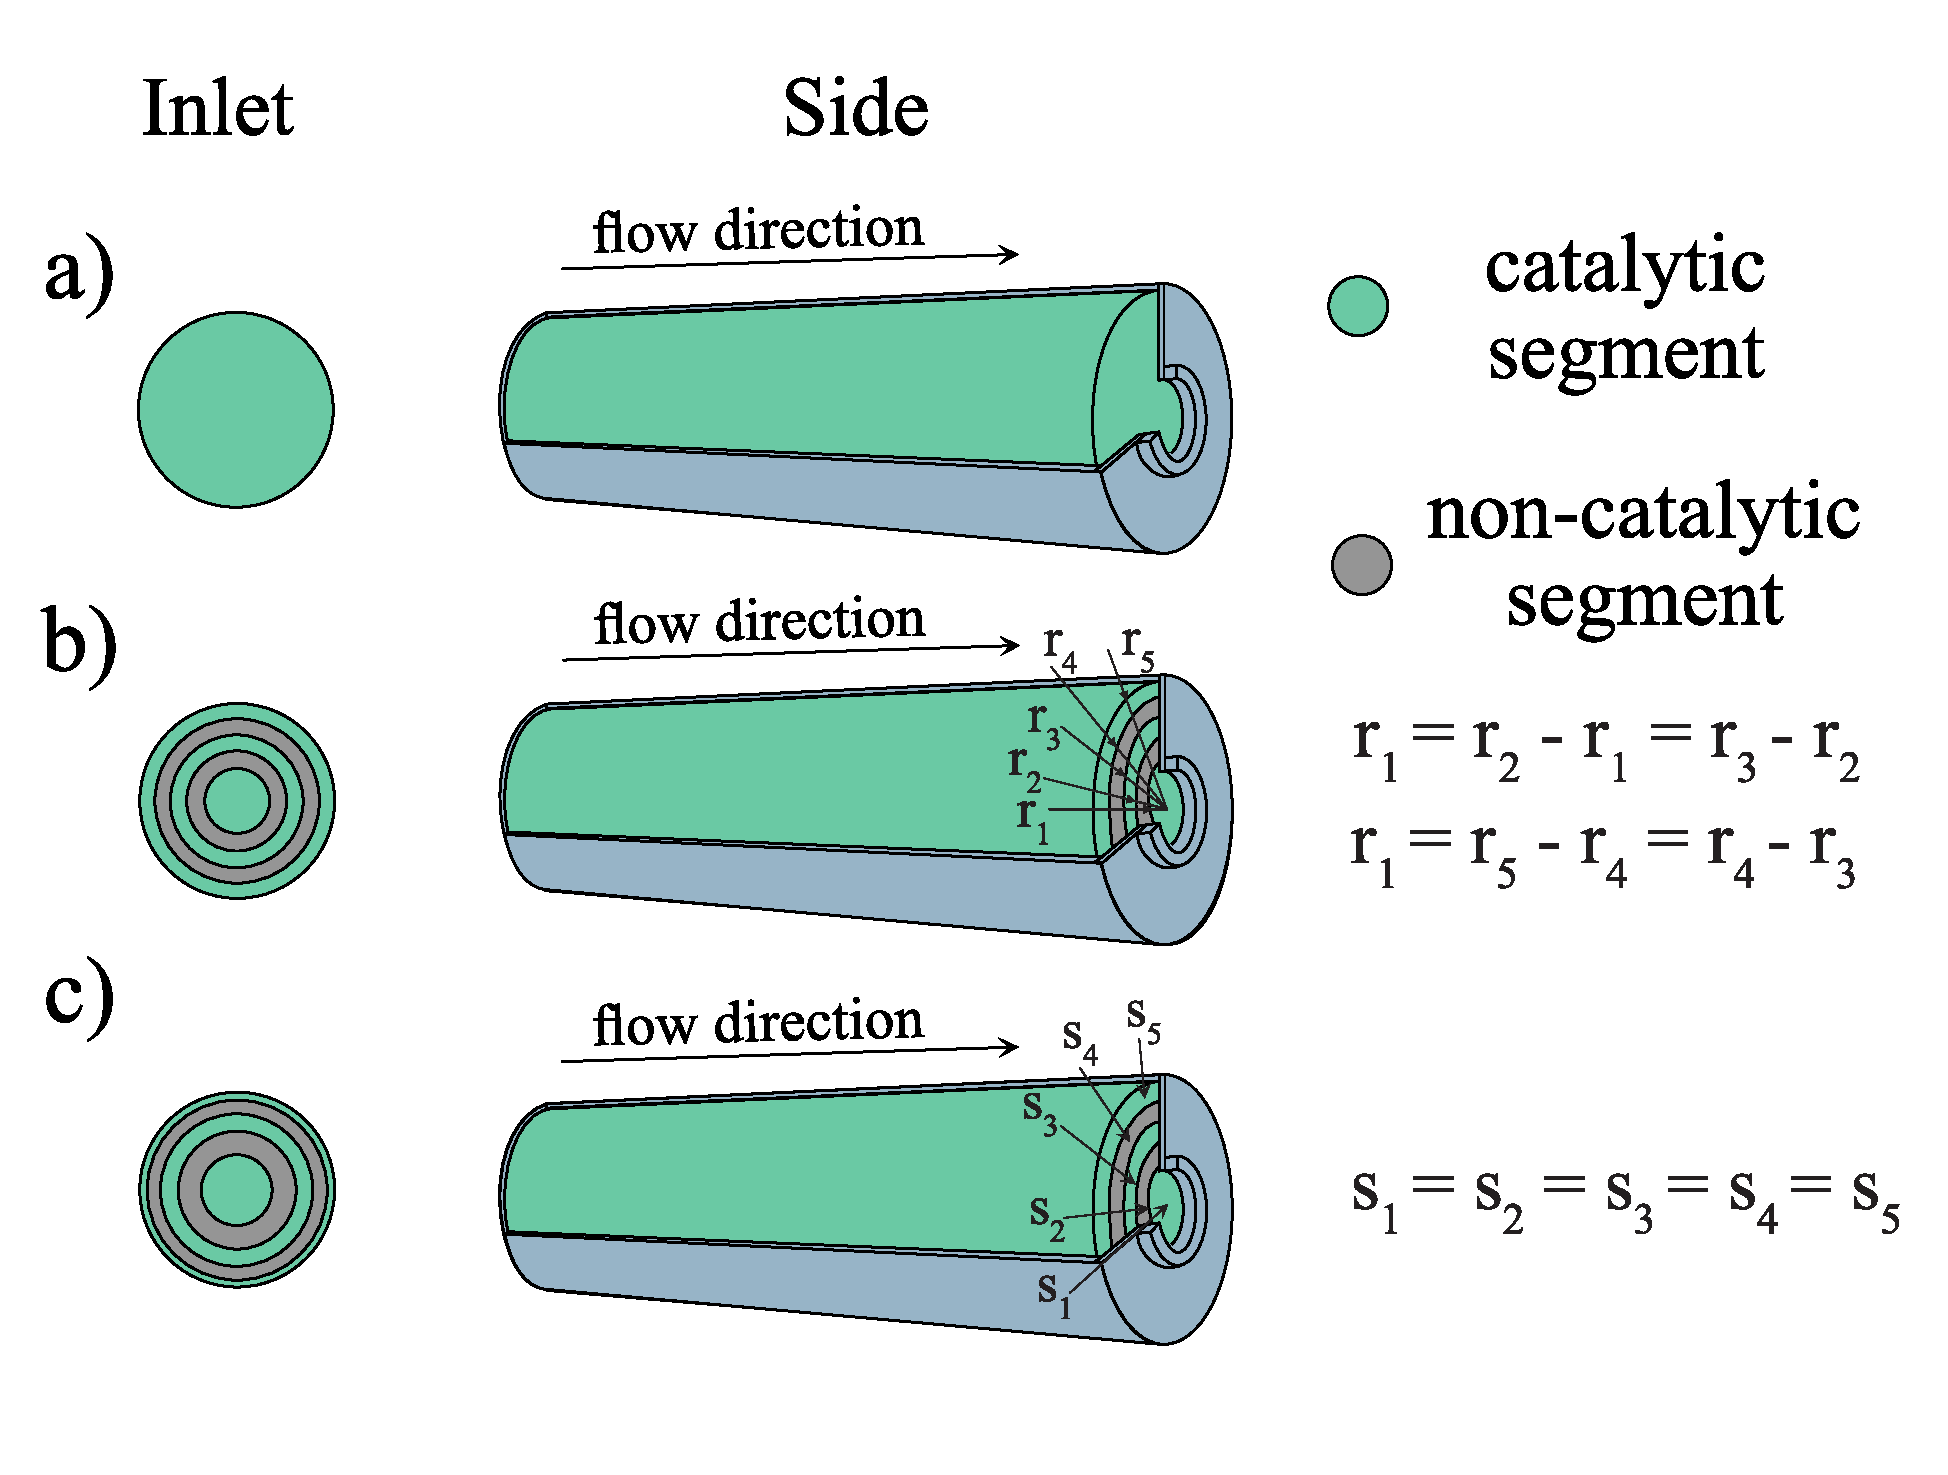
\includegraphics[width=120mm]{segments.eps}\hspace{2pc} 
\caption{\label{fig:segments} The investigated macro-patterinig designs: a) conventional reactor with homogeneous and continuous catalytic insert, b) catalytic insert divided in the radial direction (equal width of inlet surface),  c) catalytic insert divided in the radial direction  (equal area of inlet surface)}
\end{figure}
 
\subsection{Chemical Reactions Model}
\label{subsec:math_model_ref}

The process is assumed to be dominated by three reactions, as reported in literature \cite{Xu1989, Komatsu2009, Mozdzierz2018}. The reactions are steam reforming of methane (MSR) (Eq. \eqref{eq:MSR}), dry reforming of methane (DRY) (Eq. \eqref{eq:DRY}), and water-gas shift reaction (WGS) (Eq. \eqref{eq:WGS}) \cite{Brus2015}. The stoichiometric equations for the reactions are presented below: 

\begin{multline}
\label{eq:MSR}
\hfill \rm{CH_{4}+H_2O \rightarrow	3H_2+CO}, \hfill\\
{\Delta H_{\rm{MSR}} = 206.1 \rm{\frac{kJ}{mol}},}
\end{multline}
\begin{multline}
\label{eq:DRY}
\hfill \rm{CH_4+CO_2 \rightleftharpoons 2H_2+2CO}, \hfill\\
{\Delta H_{\rm{DRY}} = 247 \rm{\frac{kJ}{mol}},}
\end{multline}
\begin{multline}
\label{eq:WGS}
\hfill \rm{CO+H_2O \rightleftharpoons H_2+CO_2}, \hfill\\
{\Delta H_{\rm{WGS}} = -41.15 \rm{\frac{kJ}{mol}}.}
\end{multline}

 The reformer is supplied with a mixture of H$_2$, CO$_2$, and CH$_4$. The composition of the feedstock is determined the steam-to-carbon ratio ($SC$) parameter, defining the ratio of steam to methane provided at the reactor's inlet. The process conditions are remarkably influenced by the $SC$ value, as the reactions' rates depend directly on the composition of the inlet gases \cite{Usman2015}. A proper setting of the $SC$ is crucial for the prevention of the carbon deposition phenomenon \cite{Koncewicz2021}. Adverse process conditions can result in carbon particles precipitating on the catalyst surface \cite{Kaczmarczyk2021}. A proper setting of the ratios and the process' temperature are proven to have the most significant influence on the alleviation of the poisoning hazard \cite{Tomiczek2017}. The enthalpy changes $\Delta H$ are taken from literature \cite{Pajak2018, Mazhar2021}. Knowledge of their rates is essential to allow the inclusion of the reactions into the model. According to the research conducted by Brus et al. \cite{Brus2012}, the effective rate of MSR and DRY reactions can be expressed with a common equation:

\begin{equation}
\label{eq:rate_eff}
R_{\rm{eff}}=\dot{w}_{\rm{cat}} A_{\rm{MSR}} \exp \left(-\frac{E_{\rm{a}}}{\overline{R}T}  \right) p_{\rm{CH_4}}^\alpha \left(p_{\rm{H_2O}} + p_{\rm{CO_2}}\right)^\beta.
\end{equation}
 
 \vspace{3mm}
 
 The individual reaction rates for the MSR and DRY reactions can be distinguished as follows: 
\begin{equation}
\label{eq:rate_MSR}
R_{\rm{MSR}} = R_{\rm{eff}}\frac{p_{\rm{H_2O}}}{p_{\rm{CO_2}} + p_{\rm{H_2O}}},
\end{equation}

\begin{equation}
\label{eq:rate_DRY}
R_{\rm{DRY}} = R_{\rm{eff}}\frac{p_{\rm{CO_2}}}{p_{\rm{CO_2}} + p_{\rm{H_2O}}}.
\end{equation}

\vspace{3mm}
 
The reforming reaction is reported to occur rather slowly \cite{Brus2012JPCS}. However, the WGS reaction has a more unpredictable nature \cite{Nagata2001}. Thus, the preparation of a formula, returning proper values regardless of the process conditions, is not feasible. According to Ahmed and F\"{o}ger, the WGS reaction can be assumed to maintain equilibrium under specific conditions \cite{Ahmed2001}. The equilibrium assumption has been successfully applied in other numerical analyses \cite{Iwai2011, Sciazko2014IJHE, Peng2022}. The assumption also meets a good agreement between the calculations and the experimental data \cite{Brus2012IJHE, Sciazko2013, Sciazko2014JPS}. Taking into account the provided literature review, the WGS reaction is assumed to be in the equilibrium state in the presented analysis. The process conditions are designed to satisfy the equilibrium assumption. Following the statements, CO, CO$_{2}$, H$_{2}$ and H$_{2}$O have to satisfy the equilibrium equation, expressed by the following formula:  

\begin{equation} 
\label{eq:K_WGS}
K_{\rm{WGS}} = \dfrac{ k_{\rm{WGS}}^+}{k_{\rm{WGS}}^-} = \dfrac{p_{\rm{CO_2}} p_{\rm{H_2}}}{p_{\rm{CO}} p_{\rm{H_2O}}} = \exp \left( -\dfrac{\Delta G_{\rm{WGS}}^0}{\overline{R}T} \right).
 \end{equation}

\vspace{3mm}

The WGS reaction rate can be further expressed using Eq. \eqref{eq:rate_WGS1}:

\begin{equation}
\label{eq:rate_WGS1}
R_{\rm{WGS}} = k_{\rm{WGS}}^+ p_{\rm{CO}}p_{\rm{H_2O}} + k_{\rm{WGS}}^- p_{\rm{H_2}}p_{\rm{CO_2}}.
\end{equation}

The value of $R_{\rm{WGS}}$ can be acquired through the analysis of the reforming process stoichiometry and balancing the chemical species \cite{Brus2014, Wolf2021}.  Balancing the reaction's stoichiometry allows for the calculation of the partial pressures included in Eq. \eqref{eq:K_WGS}, leading to the relation describing the WGS reactions' rate (Eq. \eqref{eq:WGS_rate_ini}) \cite{Brus2012}.

\begin{equation}
\label{eq:WGS_rate_ini}
R_{\rm{WGS}} = \frac{n^{\rm{outlet}}_{\rm{CH_4}}}{V} = \frac{n^{\rm{inlet}}_{\rm{CH_4}} \cdot xcr}{V} ycr.
\end{equation}

\vspace{3mm}

 Following, the methane conversion rate $xcr$ and carbon monoxide conversion rate $ycr$ can be specified with:

\begin{equation}
\label{eq:ch4_conv}
xcr = 1 - \frac{n^{\rm{inlet}}_{\rm{CH_4}} - R_{\rm{MSR}}V}{n^{\rm{inlet}}_{\rm{CH_4}}},
\end{equation}

\begin{equation}
\label{eq:co_conv}
ycr = \frac{K_{\rm{WGS}} + 3xcr - \sqrt{\chi - \omega}}{2(K_{\rm{WGS}} - 1)},
\end{equation}

\noindent where:

\begin{equation}
\chi = (K_{\rm{WGS}}SC+3xcr)^2,
\end{equation}

\begin{equation}
\omega = 4K_{\rm{WGS}}xcr(K_{\rm{WGS}} - 1)(SC - xcr).
\end{equation}

Coupling Eq. \eqref{eq:ch4_conv} with Eq. \eqref{eq:WGS_rate_ini} and applying simple mathematical transformations results in the formulation of a final expression for the WGS reaction's rate:

\begin{equation}
\label{eq:rate_WGS}
R_{\rm{WGS}} = R_{\rm{MSR}}ycr.
\end{equation}

The mass consumption and production rates of the reforming process reactions (Eqs. \eqref{eq:MSR} - \eqref{eq:WGS}), are summarized in the Table \ref{tab:mass_source}. The values are further applied to the mass transfer equation (Eq. \eqref{eq:mass}), as a part of its source terms. The  heat generation rates by the described reactions are calculated depending on the rates of the reactions (Eqs. \eqref{eq:rate_MSR}, \eqref{eq:rate_DRY}, \eqref{eq:rate_WGS}) and the values of enthalpy change $\Delta H$ \cite{Xu1989, Brus2012}. The heat generation rates are given below: 

\begin{equation}
 \label{eq:q_MSR}
Q_{\rm{MSR}} = -\Delta H_{\rm{MSR}}R_{\rm{MSR}},
\end{equation}

\begin{equation}
 \label{eq:q_DRY}
Q_{\rm{DRY}} = -\Delta H_{\rm{DRY}}R_{\rm{DRY}},
\end{equation}

\begin{equation}
 \label{eq:q_WGS}
Q_{\rm{WGS}} = -\Delta H_{\rm{WGS}}R_{\rm{WGS}}.
\end{equation}
  
\vspace{\fill}

\subsection{Heat and Mass Transfer Model}
\label{subsec:heat_model}

The fundamental transport equations are incorporated into the mathematical model. Considering the computational domain defined for the needs of the analysis, the equations are implemented for two dimensions. Therefore, the model's equations are solved along the axis and radius of the reactor's geometry. The volume-averaging method was chosen for the derivation of the governing equations implemented in the model used for this analysis. The process parameters are locally averaged for each representative volume and included in the mathematical formulas \cite{Carbonell1984}. Values of continuity \linebreak (Eq. \eqref{eq:continuity}), mass transfer (Eq. \eqref{eq:mass}), momentum (Eqs. \eqref{eq:velocity_x} and \eqref{eq:velocity_r}) and energy equations (Eq. \eqref{eq:energy}) characterize the transport phenomena occurring during the reforming process. The equations are derived for the laminar flow. The analyzed fluids are considered to be Newtonian and incompressible. Thus, the continuity equation takes the following form \cite{Nishino2003, Nishino2006}: 

\begin{equation}
\label{eq:continuity}
 \frac {\partial \left( \rho_0 U_x  \right) }{\partial x}+\frac {1}{r} \frac {\partial \left(  r \rho_0 U_r  \right) }{\partial r}=0,
\end{equation}

\vspace{3mm}
  
 The species conservation is calculated using molar fractions of species taking part in the reaction (Equation \eqref{eq:mass}). The formulated equation is derived from Fick's law of diffusion~\cite{Mozdzierz2018}. The mass sources and sinks $S_j$ depend on the MSR, DRY, and WGS rates and molar masses of the species taking part in the reaction~\cite{Mozdzierz2014, Tan2018}.  The exact equations defining the values of $S_j$ are described in Table \ref{tab:mass_source}. 
   
\begin{eqnarray} 
\label{eq:mass}
\begin{multlined}
 \rho_0   \left( U_x \frac{\partial  Y_{j}}{\partial x} +   U_r \frac{\partial  Y_{j}}{\partial r} \right) = \frac {\partial}{\partial x} \left( \rho_0 D_{j, \rm{eff}}  \frac{\partial  Y_{j}}{\partial x} \right) \\
 + \frac{1}{r} \frac {\partial}{\partial r} \left( r \rho_0 D_{j, \rm{eff}}  \frac{\partial  Y_{j}}{\partial r} \right) + S_{j}.
 \end{multlined}
 \end{eqnarray}
 
 \begin{table}
\renewcommand{\arraystretch}{1.7}
\caption{Mass sources/sinks}
\label{tab:mass_source}       
\centering
\begin{tabular}{l||p{0.2\linewidth}|p{0.2\linewidth}|p{0.2\linewidth}|p{0.2\linewidth}}

\toprule

species & mass generation MSR  & mass generation WGS  & mass generation DRY & summarized \linebreak  generation \\

\midrule

$\rm{H}_2$ & $3R_{\rm{MSR}}M_{\rm{H_2}}$ & $R_{\rm{WGS}}M_{\rm{H_2}}$ & $2R_{\rm{DRY}}M_{\rm{H_2}}$ & $3R_{\rm{MSR}}M_{\rm{H_2}}\linebreak\indent +R_{\rm{WGS}}M_{\rm{H_2}}$ \linebreak\indent + $2R_{\rm{DRY}}M_{\rm{H_2}}$ \\

\noalign{\smallskip}\hline\noalign{\smallskip}

CO & $R_{\rm{MSR}}M_{\rm{CO}}$ & $-R_{\rm{WGS}}M_{\rm{CO}}$ & $2R_{\rm{DRY}}M_{\rm{CO}}$ & $R_{\rm{MSR}}M_{\rm{CO}} \linebreak\indent -R_{\rm{WGS}}M_{\rm{CO}}$  + $2R_{\rm{DRY}}M_{\rm{CO}}$\\

\noalign{\smallskip}\hline\noalign{\smallskip}

$\rm{CO_2}$ & 0 & $R_{\rm{WGS}}M_{\rm{CO_2}}$ & $-R_{\rm{DRY}}M_{\rm{CO_2}}$ & $R_{\rm{WGS}}M_{\rm{CO_2}}$ \linebreak\indent $-2R_{\rm{DRY}}M_{\rm{H_2}}$ \\

\noalign{\smallskip}\hline\noalign{\smallskip}

$\rm{CH_4}$ & $-R_{\rm{MSR}}M_{\rm{CH_4}}$ & 0 & $-R_{\rm{DRY}}M_{\rm{H_2}}$ & $-R_{\rm{MSR}}M_{\rm{CH_4}}$ \linebreak $-R_{\rm{DRY}}M_{\rm{H_2}}$ \\

\noalign{\smallskip}\hline\noalign{\smallskip}

$\rm{H_2O}$ & $-R_{\rm{MSR}}M_{\rm{H_2O}}$ & $-R_{\rm{WGS}}M_{\rm{H_2O}}$ & 0 & $-R_{\rm{MSR}}M_{\rm{H_2O}}$ 
$-R_{\rm{WGS}}M_{\rm{H_2O}}$ \\
\bottomrule

\end{tabular}
\end{table}


 

The effective mass diffusivity of species $D_{j\rm{eff}}$ was calculated using the equation explained below (Eq. 
\eqref{eq:diff}) \cite{Suzuki2005}:

\begin{equation}
\label{eq:diff}
 	 D_{j\rm{,eff}} = (1-\sqrt{1-\varepsilon})D_{j}.
\end{equation}

\vspace{3mm} 

The diffusion of substance $j$ in the gas mixture $D_{j}$ is computed using Fuller's method and Blanc's law. The gases' properties are taken from the literature \cite{PolingB.E.;Prausnitz2001}. The values assumed for the flow model describe the local phase average of the gas control volume.
 The momentum conservation depends directly on the insert's morphology. The materials composing the insert are considered porous. Therefore,  parameters describing the material structure have to be included in the equations. The parameters are porosity $\varepsilon$, permeability $K_p$, and inertial coefficient $c_{\rm{ine}}$ \cite{Pajak2021IJHEb}. A separate momentum equation is formulated for each of the computational domain dimensions (Eqs. \eqref{eq:velocity_x} and \eqref{eq:velocity_r}). 

\begin{eqnarray} 
\begin{multlined}
\label{eq:velocity_x}
 \frac{ \rho_0}{  \varepsilon^2_0} \left( U_x \frac {\partial U_x}{\partial x} + U_r \frac {\partial U_x}{\partial r} \right)  =  - \frac{\partial P}{\partial x} +\frac{\mu}{ \varepsilon}   \left[ \frac {\partial^2 U_x}{\partial x^2} + \frac {1}{r} \frac {\partial}{\partial r} \left( r \frac {\partial U_x}{\partial r} \right) \right]   \\
 - \frac{ \mu}{ K_{\rm{p}} } U_x - \frac{ \rho_0 c_{\rm{ine}} }{ \sqrt{ K_{\rm{p}} }} U_x \sqrt {U^2_x + U^2_r},
 \end{multlined}
 \end{eqnarray}
 
 \begin{eqnarray} 
\begin{multlined}
\label{eq:velocity_r}
 \frac{ \rho_0}{  \varepsilon^2_0} \left( U_x \frac {\partial U_r}{\partial x} + U_r \frac {\partial U_r}{\partial r} \right)  =  - \frac{\partial P}{\partial r} +\frac{\mu}{ \varepsilon}   \left[ \frac {\partial^2 U_r}{\partial x^2} + \frac {1}{r} \frac {\partial}{\partial r} \left( r \frac {\partial U_r}{\partial r} \right) - \frac {U_r}{r^2} \right]   \\
   - \frac{ \mu}{ K_{\rm{p}} } U_r - \frac{ \rho_0 c_{\rm{ine}} }{ \sqrt{ K_{\rm{p}} }} U_r \sqrt {U^2_x + U^2_r}.
   \end{multlined}
 \end{eqnarray}
 
 \vspace{3mm}
 
 The permeability $K_{\rm{p}}$ of the specific segment is calculated using \eqref{eq:perm}, basing on the information about its porosity $\varepsilon$ \cite{Yang2014}:

\begin{equation}
\label{eq:perm}
K_{\rm{p}} = \frac{\varepsilon(1-(1-\varepsilon)^{1/3})}{36((1-\varepsilon)^{1/3}-(1-\varepsilon))}d_{\rm{p}}^2,
\end{equation}

\vspace{3mm}

where $d_{\rm{p}}$ stands for an average pore diameter. The inertial coefficient $c_{\rm{ine}}$ was calculated using \cite{Bhattacharya2002}:

\begin{equation}
\label{eq:inert_coef}
c_{\rm{ine}} = 0.0095g_{\rm{s}}^{-0.8}\sqrt{\frac{\varepsilon}{3(\tau-1)}}(1.18\sqrt{\frac{(1-\varepsilon)}{3\pi}}\frac{1}{g_{\rm{s}}})^{-1},
\end{equation}

\vspace{3mm}

where tortousity $\tau$ and and shape function $g_{\rm{s}}$ are expressed with following equations \cite{Yang2014, Bhattacharya2002}:

\begin{equation}
\label{eq:tortuosity}
\tau = \frac{\varepsilon}{1-(1-\varepsilon)^{1/3}},
\end{equation}

\begin{equation}
\label{eq:shape_func}
g_{\rm{s}} = 1 - \exp(-\frac{1-\varepsilon}{0.04}).
\end{equation}

\vspace{3mm}

The energy conservation equation (Eq. \eqref{eq:energy}) describes the process of heat transfer during the reaction. The equation includes local thermal conditions, the materials' parameters, and the heat sources calculated using Eqs. \eqref{eq:q_MSR} - \eqref{eq:q_WGS}. 

\begin{eqnarray} 
\label{eq:energy}
 \rho_0 C_{p} \left( U_x \frac{\partial T_{\rm{loc}}}{\partial x} + U_r \frac{\partial T_{\rm{loc}}}{\partial r} \right)  = \frac {\partial}{\partial x} \left( \lambda_{\rm{eff}}  \frac {\partial T_{\rm{loc}}}{\partial x}  \right) + \frac {1}{r} \frac {\partial}{\partial r} \left( r \lambda_{\rm{eff}}  \frac {\partial T_{\rm{loc}}}{\partial r}  \right) + Q_{\rm{s}}.
 \end{eqnarray} 

\vspace{3mm}

Due to the application of metallic foam, a proper relation describing the $\lambda_{\rm{eff}}$ of the material is essential \cite{Bhattacharya2002}.  The model chosen for calculating the value of the $\lambda_{\rm{eff}}$ was proposed by Boomsma and Poulikakos and further corrected by Dai et al. \cite{Boomsma2001, Dai2010}. The outcome relation allows for the derivation of equations describing the thermal conductivity of metallic foams. According to the literature review, an adequate model including the morphology of metallic foams is prepared \cite{Pajak2021IJHEa}.
 
\begin{equation}
\label{eq:eff_cond} 
\lambda_{\rm{eff}}=\frac{\sqrt{2}l}{2(R_{\rm{A}}+R_{\rm{B}}+R_{\rm{C}}+R_{\rm{D}})},
\end{equation}

\vspace{3mm}
\noindent where $R_{\rm{A}}$ - $R_{\rm{D}}$ stand for the thermal resistances of the porous media cell subsections \cite{Pajak2018, Dai2010}.


\section{Numerical model}
\label{sec:num_model}

To solve systems of the defined equations a discretization of the previously prepared continuous computational domain is necessary. The numerical model is prepared using the Finite Volume Method \cite{Moukalled2016}.  A uniform computational grid with evenly spaced nodes is formed, to assure a minimal complexity of the calculations, \cite{Kaw2011}. The grid's dimensions are established at 150 elements in the longitudinal and 25 elements in the radial directions, resulting in square-shaped elements. A single grid sector is presented in Fig. \ref{fig:grid} 

\begin{figure}[h]
\centering
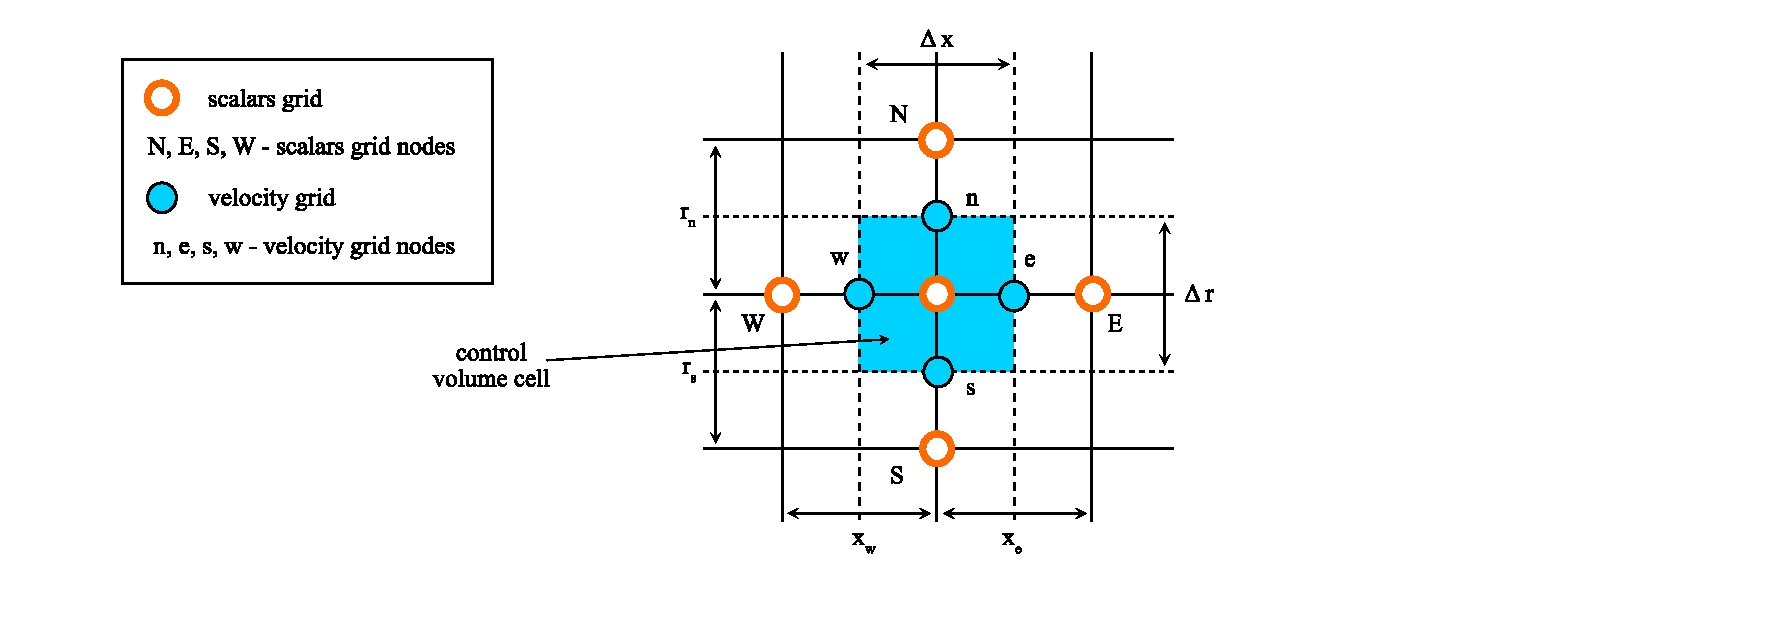
\includegraphics[width=180mm]{grid.eps}\hspace{2pc} 
\caption{\label{fig:grid} Numerical grid implemented in the analysis}
\end{figure}

\subsection{Transport Equations}
\label{sec:trans_eqs}

Integration of the fundamental transport equations of the reforming process over the created control volumes is conducted \cite{Patankar1980}.  The partial differential equations covering the species conservation (Eq. \eqref{eq:mass}),  the momentum conservation equation (Eqs. \eqref{eq:velocity_x} - \eqref{eq:velocity_r}), and the energy conservation equation (Eq. \eqref{eq:energy}) may be described in a generalized form \cite{Patankar1980}, as follows: 


\begin{equation}
\label{eq:general}
\varPsi_x \dfrac{\partial \phi}{\partial x} + \varPsi_r \dfrac{\partial \phi}{\partial r} = \dfrac{\partial}{\partial x} \left( \varGamma \dfrac{\partial \phi}{\partial x} \right) + \dfrac{1}{r} \dfrac{\partial}{\partial r} \left( r \varGamma \dfrac{\partial \phi}{\partial r} \right) + \overline{S}.
\end{equation}
\hspace{\fill}

The Eq. \eqref{eq:general} is prepared to allow substitution of any dependant variable $\phi$. The coefficients on the left side of the Eq. \eqref{eq:general}, $\varPsi_x$ and $\varPsi_r$ describe the convective terms in $x$ and $r$ directions and may be substituted accordingly to the use case. The diffusive terms, represented by $\varGamma$, are placed on the right-hand side of the equation, along with the source terms $\overline{S}$.  The corresponding terms and coefficients are summarized in Tab. \ref{tab:coeff}. The source terms $\overline{S}$ values regard the catalytic segments only. The reaction is assumed to be put to a halt for the non-catalytic region of the insert. Therefore, no heat and mass production nor consumption is predicted for the metallic foam segments.
 
\begin{table}
\caption{Coefficients and terms for substitution in Eq. \eqref{eq:general}}
\label{tab:coeff}
\begin{tabular}{l|c|c|c|c|c}
\hline\noalign{\smallskip}
Eq. & $\phi$ & $\varPsi_x$ & $\varPsi_r$ & $\varGamma$ & $\overline{S}$  \\
\noalign{\smallskip}\hline\noalign{\smallskip}
(\ref{eq:mass}) & $Y_j$ & $\rho_0 U_x$ & $\rho_0 U_r$ & $\rho_0 D_{j,\rm{eff}}$ & $S_j$ \\
(\ref{eq:velocity_x}) & $U_x$ & $\dfrac{\rho_0}{\varepsilon^2_0} U_x$ & $\dfrac{\rho_0}{\varepsilon^2_0} U_r$ & $\dfrac{\mu}{\varepsilon_0}$ & $-\dfrac{\partial P}{\partial x} - \dfrac{\mu}{K_{\rm{p}}} U_x - \dfrac{\rho_0 c_{\rm{ine}}}{\sqrt{K_{\rm{p}}}} U_x \sqrt{U^2_x+U^2_r}$ \\
(\ref{eq:velocity_r}) & $U_r$ & $\dfrac{\rho_0}{\varepsilon^2_0} U_r$ & $\dfrac{\rho_0}{\varepsilon^2_0} U_r$ & $\dfrac{\mu}{\varepsilon_0}$ & $-\dfrac{\partial P}{\partial r} - \dfrac{\mu}{K_{\rm{p}}} U_r - \dfrac{\rho_0 c_{\rm{ine}}}{\sqrt{K_{\rm{p}}}} U_r \sqrt{U^2_x+U^2_r} - \dfrac{\mu U_r}{\varepsilon_0 r^2}$ \\
(\ref{eq:energy}) & $T$ & $\rho_0 C_{\rm{p}} U_x$ & $\rho_0 C_{\rm{p}} U_r$ & $\lambda_{\rm{eff}}$ & $Q_{\rm{s}}$ \\

\noalign{\smallskip}\hline
\end{tabular}
\end{table}

\subsection{Coaxial segments configuration}

The reactor has been divided into five concentric segments, constituting four hollow cylinders and a core. The segments may take one of two configurations. The first one predicts equal width of the inlet and outlet surfaces, while the second configuration predicts an equal area of inlet and outlet surfaces. The two possible setups are summarized in Fig. \ref{fig:inlet_rings}.  

\begin{figure}[h]
\centering
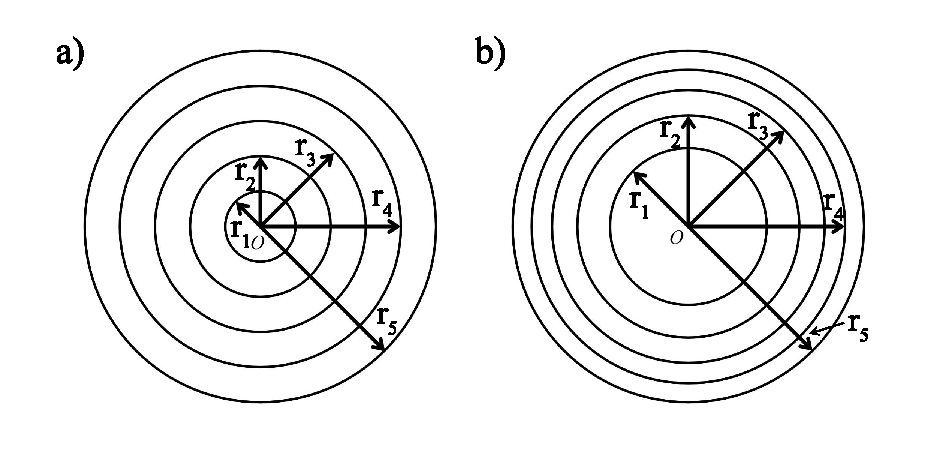
\includegraphics[width=120mm]{reactor_inlet_surface.eps}\hspace{2pc} 
\caption{\label{fig:inlet_rings} The coaxial segments configurations: a) equal width of rings, b) equal inlet and outlet surface}
\end{figure}

The exact dimensions of the particular rings for Fig. \ref{fig:inlet_rings} b) are calculated using the system of equations \eqref{eq:rings}, as follows:

\begin{equation}
\centering
\label{eq:rings}
\begin{cases}
	2\pi r_1^2 = \frac{2}{5}\pi R^2 \\
	2\pi \left(r_2^2 - r_1^2 \right) = \frac{2}{5}\pi R^2 \\
	2\pi \left(r_3^2 - r_2^2 \right) = \frac{2}{5}\pi R^2 \\
	2\pi \left(r_4^2 - r_3^2 \right) = \frac{2}{5}\pi R^2 \\
	2\pi \left(r_5^2 - r_4^2 \right) = \frac{2}{5}\pi R^2	
\end{cases}
\end{equation}

\vspace{3mm}

The values resulting from solving the Eqs. \eqref{eq:rings} are presented in Tab. \ref{tab:rings_radius}.  


\begin{table}[h]
\centering
\caption{Rings' dimensions}
\label{tab:rings_radius}
\begin{tabular}{c||c|c}
\hline\noalign{\smallskip}
Radius & Equal width (cm) & Equal surface (cm) \\
\noalign{\smallskip}\hline\noalign{\smallskip}
r$_1$ & 1 & $\sqrt{5}$ \\
\noalign{\smallskip}\hline\noalign{\smallskip}
r$_2$ & 2 & $\sqrt{10}$  \\
\noalign{\smallskip}\hline\noalign{\smallskip}
r$_3$ & 3 & $\sqrt{15}$  \\
\noalign{\smallskip}\hline\noalign{\smallskip}
r$_4$ & 4 & $2\sqrt{5}$ \\
\noalign{\smallskip}\hline\noalign{\smallskip}
r$_5$ & 5 & 5 \\
\noalign{\smallskip}\hline
\end{tabular}

\end{table}

The computational domain is indicated with the red dashed line (Fig. \ref{fig:comp_domain}). Segments can be described with the following parameters - porosity, average pore size, as well as their catalytic properties, which are directly correlated to the porosity value. The analyzed model is steady and the flow of gases is assumed to be laminar and occurring in one direction. Fluids taking part in the process are assumed to be Newtonian. The presented numerical analysis is a quasi-three-dimensional case. Due to the axial symmetry of the reactor's tube, a computational domain can be constrained to a two-dimensional cross-section of the reformer. Implementation of proper boundary conditions allows assuming the process occurs in the same manner throughout the reactor's whole volume \cite{Patankar1980}. 


\begin{figure}[h]
\centering
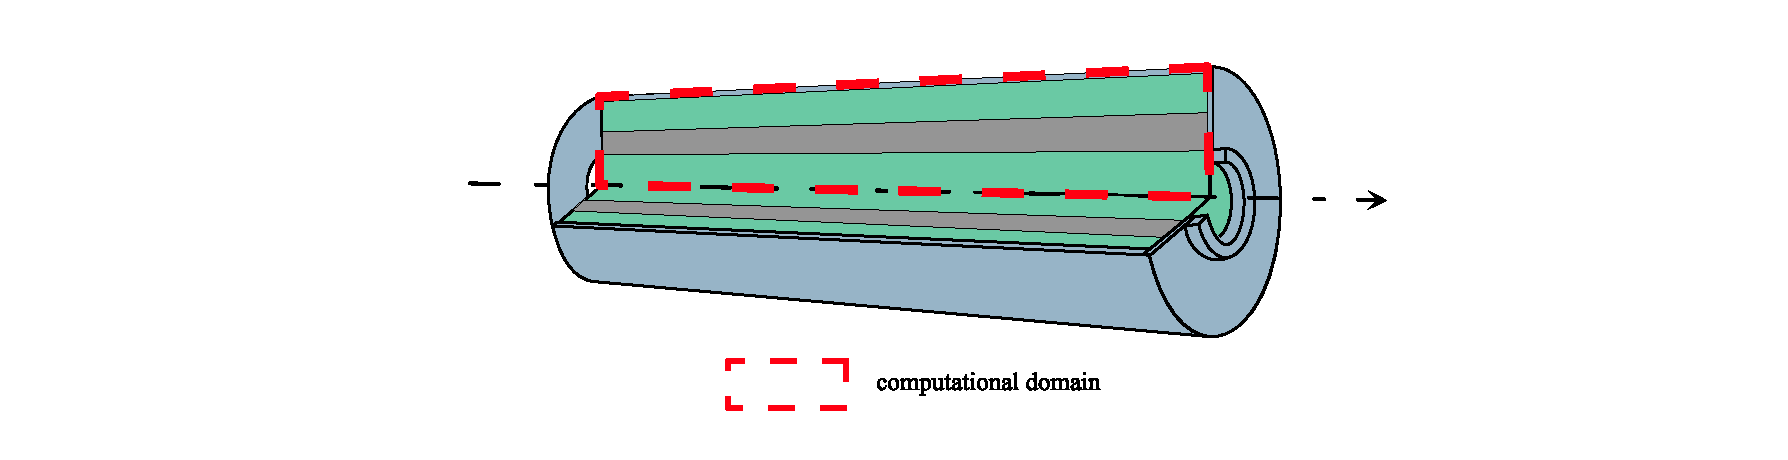
\includegraphics[width=120mm]{domain.eps}\hspace{2pc} 
\caption{\label{fig:comp_domain} Quasi 3-dimensional computational domains for the rings configurations}
\end{figure}

\subsection{Boundary Conditions and Materials}
\label{sec:boundary}

To complete the preparation of the numerical analysis, setting the properties of the materials and the boundary conditions is vital. Proper setting of $\textit{SC}$ value is essential for this analysis, due to the threat of carbon deposit formation \cite{Bartholomew1982}. If the ratios are chosen incorrectly, the carbon deposition phenomenon may occur, poisoning the reactor's catalyst \cite{Lakhapatri2009}. Choosing an appropriate steam-to-carbon ratio allows for avoiding the described hazard. The value of \textit{SC} for this analysis was set to be equal to 2.0 [-], preventing this occurrence \cite{Brus2015, Tomiczek2017}. The catalyst insert's segments are assumed to consist of one of two materials. The first material is a catalytic composite of nickel and yttria-stabilized-zirconia (Ni/YSZ). The second material, serving the purpose of heat transport medium, is chosen to be steel foam. The metallic foam segments are introduced for the unification of the temperature distribution inside the reactor.  Suppression of the reforming reaction, combined with a considerable heat exchange surface for foams, is expected to let the gases mixture reheat effectively \cite{Zhao2012}. The value of $\lambda_{\rm{solid}}$ is set at 22 W m$^{-1}$ K$^{-1}$ for the catalytic material \cite{Kawashima1996}, while the value of $\lambda_{\rm{solid}}$ for the steel foam is established at 30 W m$^{-1}$ K$^{-1}$ \cite{Peet2011}. The dimensionless cubic node length $e$ is set to be equal to 0.0339, as explained by Boomsma and Poulikakos \cite{Boomsma2001}.  The temperature of the fuel flowing inside the unit is considered to reach the temperature of the reformer instantly. The symmetry boundary conditions are set at the symmetry axis, while the no-slip boundary condition is applied at the wall of the reformer. The boundary conditions necessary for the solution of the governing equations are summarized below.

\subsection*{Thermal Boundary Conditions}
\begin{itemize}
  \item inlet temperature $T = T_{\rm{in}} = 900$ K \hspace*{\fill} \hfill at $x = 0$ and $0 \leq r < R$,
  \item outlet temperature $\partial T / \partial x = 0$ \hspace*{\fill} \hfill at $x = L$ and $0 \leq r < R$,
  \item symmetry boundary condition $\partial T / \partial r = 0$ \hspace*{\fill} \hfill at $0 \leq x < L$ and $r = 0$,
  \item wall heat flux $\partial T / \partial r =  const$ \hspace*{\fill} \hfill at $0 \leq x < L$ and $r = R$.
\end{itemize}

The thermal boundary condition set at the reactor's wall is chosen to be of a second type. Constant heat flux is assumed on the reactor's wall, and the wall itself is the medium for heat exchange between the reactor and the system boundaries. The wall thickness is set to be equal to 0.001 m and is assumed to consist of the same material as the metallic foams. Thus, the value of $\lambda_{\rm{solid}}$ for the reactor's wall is equal to  30 W m$^{-1}$ K$^{-1}$ \cite{Peet2011}. The boundary conditions essential for the calculation of the species conservation equations are presented below. 

\subsection*{Mass Transport Boundary Conditions}
\begin{itemize}
  \item inlet mole fractions $Y_j = Y_{j,\rm{in}}$ \hspace*{\fill}  at $x = 0$ and $0 \leq r < R$,
  \item outlet mole fractions $\partial Y_j / \partial x = 0$ \hspace*{\fill} \hfill at $x = L$ and $0 \leq r < R$,
  \item symmetry boundary condition $\partial Y_j / \partial r = 0$ \hspace*{\fill} \hfill at $0 \leq x < L$ and $r = 0$,
  \item no-slip boundary condition $Y_j = 0$ \hspace*{\fill} \hfill at $0 \leq x < L$ and $r = R$.
\end{itemize}

To complete the numerical model's setting, the boundary conditions for solving the momentum conservation equations are needed. The conditions are applied in the manner listed below. 

\subsection*{Momentum Boundary Conditions}
\begin{itemize}
  \item inlet velocity $U = U_{\rm{in}} = 0.15$ m s$^{-1}$ \hspace*{\fill} \hfill at $x = 0$ and $0 \leq r < R$,
  \item outlet velocity $\partial U / \partial x = 0$ \hspace*{\fill} \hfill at $x = L$ and $0 \leq r < R$,
  \item symmetry boundary condition $\partial U / \partial r = 0$ \hspace*{\fill} \hfill at $0 \leq x < L$ and $r = 0$,
  \item no-slip boundary condition $U = 0$ \hspace*{\fill} \hfill at $0 \leq x < L$ and $r = R$.
\end{itemize}

All of the boundary conditions are summarized in Fig. \ref{fig:boundary}.

\begin{figure}
\centering
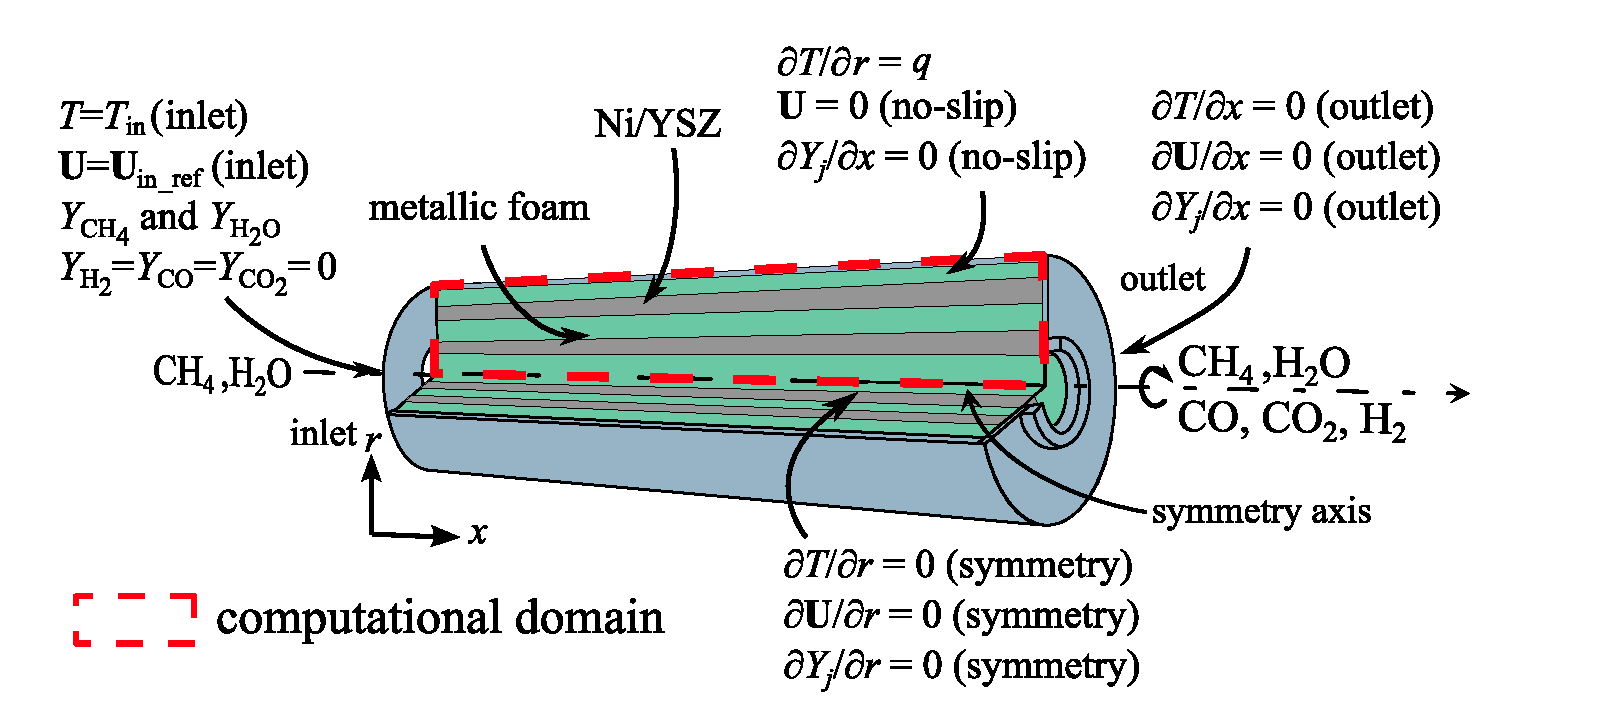
\includegraphics[width=120mm]{boundary.eps}
\caption{\label{fig:boundary}Boundary conditions applied in the analysis} 
\end{figure}

\section{Genetic algorithm}
\label{sec:ga}

The conducted optimization includes the application of an evolutionary algorithm, to define the optimal design of the catalytic insert for the coaxial segments. The genetic algorithm (GA) is selected to be the optimization procedure used for the needs of the analysis. The algorithm analyses subsequent, finite populations of test specimens, which parameters are inherited from the specimens acquiring the best results in the preceding generation. The results are evaluated by user-defined fitness functions \cite{Tai2022}. The functions are exclusive to a certain problem. If more than one function is defined, the functions have to be combined into a single value, which will be further processed by the genetic algorithm itself \cite{Goldberg1989}. The remaining part of the genetic algorithm operation is the mutation procedure. The mutation is used as an additional procedure for preventing the local extremum trap and a measure for the introduction of genes that were not present in the initial population or are just not possible to acquire on the way of the crossover procedure \cite{Raja2017}. Coupling of the prepared numerical anlysis with the algorithm requires proper parametrization of reactor parameters \cite{Goldberg1989}. The catalyst insert is set to contain 5  coaxial segments. Each of the segments is assumed to consist of either a catalytic composite of nickel with yttria-stabilized-zirconia (Ni/YSZ) or a stainless steel foam \cite{Pajak2021IJHEa}. The insert regions may differ in their morphological parameters regardless of the constituting material. The parameters altered by the algorithm are segment catalytic character, porosity $\varepsilon$ and average pore diameter $d_{\rm{p}}$. The porosity values available for application in the analysis are constrained to the range between 0.5 and 0.8. The lower boundary is set at 0.5, as lower porosity values resulted in over-significant pressure drops during the preliminary calculations.  The choice of 0.8 as the upper boundary is motivated by lower accessibility to the manufacturing methods determined for metallic foams of higher porosities \cite{Banhart2001}.  The average pore diameters $d_{\rm{p}}$ are calculated for each segment, based on the values of the porosity \cite{Pajak2021IJHEa}. The upper boundary of the $d_{\rm{p}}$ range is restricted by the model conditions. According to the volume-averaging method, the size of a single pore is not allowed to exceed the size of a single numerical grid element. Therefore, the upper boundary is limited to 0.002 m \cite{Carbonell1984} Furthermore, segment porosity $\varepsilon$ has a direct influence on the catalyst density. The catalyst density $\dot{w}_{\rm{cat}}$ is calculated using Eq. \eqref{eq:cat_dens}:

\begin{equation}
\label{eq:cat_dens}
\dot{w}_{\rm{cat}} = \rho_{\rm{cat}} \cdot (1-\varepsilon_{\rm{0}}),
\end{equation}

\noindent where $\rho_{\rm{cat}}$ is equal to $5.3448 \cdot 10^6$ g m$^{-3}$. The chemical reaction kinetics model derived for the implemented numerical simulation regards a Ni/YSZ composite with a 60:40 Ni to YSZ ratio \cite{Pajak2021IJHEa}. Nickel serves the catalytic purpose, while YSZ serves as a scaffold. Therefore, the basic catalyst density for the Ni/YSZ element should be calculated concerning the ratio of the materials. The solid nickel density equals to $8.908 \cdot 10^6$ g m$^{-3}$ \cite{Everhart2012}. The value of $\rho_{\rm{cat}}$ is calculated by applying the given ratio to the value of the solid nickel density \cite{Pajak2021IJHEa}.  The definition of the relations allows commencing the operation of the GA. The algorithm starts its operation with the preparation of the initial generation, with the specimens' parameters fully randomized. First, the segments' character is randomized. The algorithm is expected to generate catalytic and non-catalytic segments in a ratio of 50:50, as the randomization procedure uses a uniform distribution for its seed \cite{Jerrum1986}.  When the specific segment's character is determined, the algorithm randomizes its porosity  $\varepsilon$ and average pore size $d_{\rm{p}}$ values. As the final initialization step, the GA calculates the catalyst density for each of the segments designated to consist of Ni/YSZ composite. Having defined the initial parameters, the reforming simulation code is executed for each of the generated reactors.  The overall operation of the algorithm prepared for the needs of the research is presented in Fig. \ref{fig:ga}. 

\begin{figure}[h]
\centering
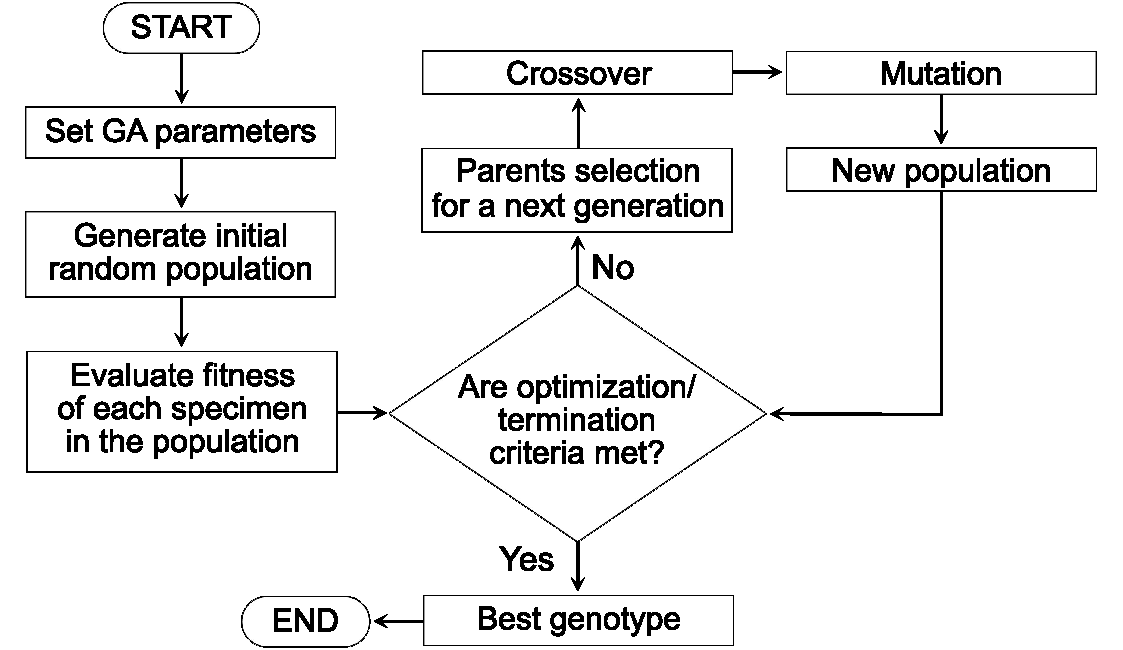
\includegraphics[width=120mm]{block_ga.eps}\hspace{2pc}
\caption{\label{fig:ga} Summary of the genetic algorithm procedure}
\end{figure}

The conducted investigation regards optimization of the temperature field distribution inside the reactor, simultaneously maintaining a considerable methane conversion rate \cite{Pajak2021IJHEb}. Therefore, the research is considered a multi-objective optimization, as the fitness analysis is required to investigate two separate factors. The first factor is temperature distribution. The main objective is to reduce the temperature gradients occurring throughout the reactor's volume during the reaction. The strong endothermic character of the process has a consequence in large temperature decreases in the regions in which the fuel concentration is significant. The constant transition of the temperature field leads to the establishment of thermal stresses, leading to premature degradation of the catalyst material \cite{Pajak2021Energies}.  The presented research predicts the search for an optimal distribution of catalytic and non-catalytic segments and proper selection of their porosity $\varepsilon$ and average pore size $d_{\rm{p}}$.  The first function $f_{\rm{CH_4}}$ regards the methane conversion rate. The fuel conversion rate is calculated using the molar fractions of the methane at the inlet and the outlet of a specific reactor. The $f_{\rm{CH_4}}$  value is calculated using Eq. \eqref{eq:fit_CH4}:

\begin{equation}
\label{eq:fit_CH4}
	f_{\rm{CH_4}} = \frac{(frac_{\rm{CH_{4in}}} - frac_{\rm{CH_{4out}}})}{frac_{\rm{CH_{4in}}}},
\end{equation}

The remaining fitness function $f_T$ evaluates the extent of the unification of the temperature distribution inside the catalytic insert. Essentially, the thermal fitness objective is to find the $\Delta T$ value, being a representative temperature difference for a specific reactor. To assure reliability and accuracy of the mathematical formula, the thermal fitness is established to perform the temperature distribution analysis for each of the grid elements separately \cite{Pajak2021IJHEb}. The algorithm iterates through each of the created control volumes and calculates the temperature difference between the central node $T_{\rm{P}}$ and each of the neighboring control volumes $T_{\rm{N}}$, $T_{\rm{E}}$, $T_{\rm{S}}$, $T_{\rm{W}}$ (Fig. \ref{fig:f_T}). Further, each of the control volumes has its specific temperature difference $\Delta T_{\rm{loc}_{\textit{i,j}}}$ assigned. The $\Delta T_{\rm{loc}_{\textit{i,j}}}$ value is chosen to be the highest temperature difference among the values calculated for each of the neighboring control volumes. The $\Delta T_{\rm{loc}_{\textit{i,j}}}$ for each of the cells is based on the following formula: 

\begin{eqnarray} 
\label{eq:DT_loc}
\begin{multlined}
\Delta T_{{\rm{loc}}_{i,j}} = \\ {\rm{max}}\left\{|T_{{\rm{P}}_{i,j}} - T_{{\rm{N}}_{i,j}}|, |T_{{\rm{P}}_{i,j}} - T_{{\rm{E}}_{i,j}}|, |T_{{\rm{P}}_{i,j}} - T_{{\rm{S}}_{i,j}}|, |T_{{\rm{P}}_{i,j}} - T_{{\rm{W}}_{i,j}}|\right\}.
 \end{multlined}
 \end{eqnarray}

\begin{figure}[h]
\centering
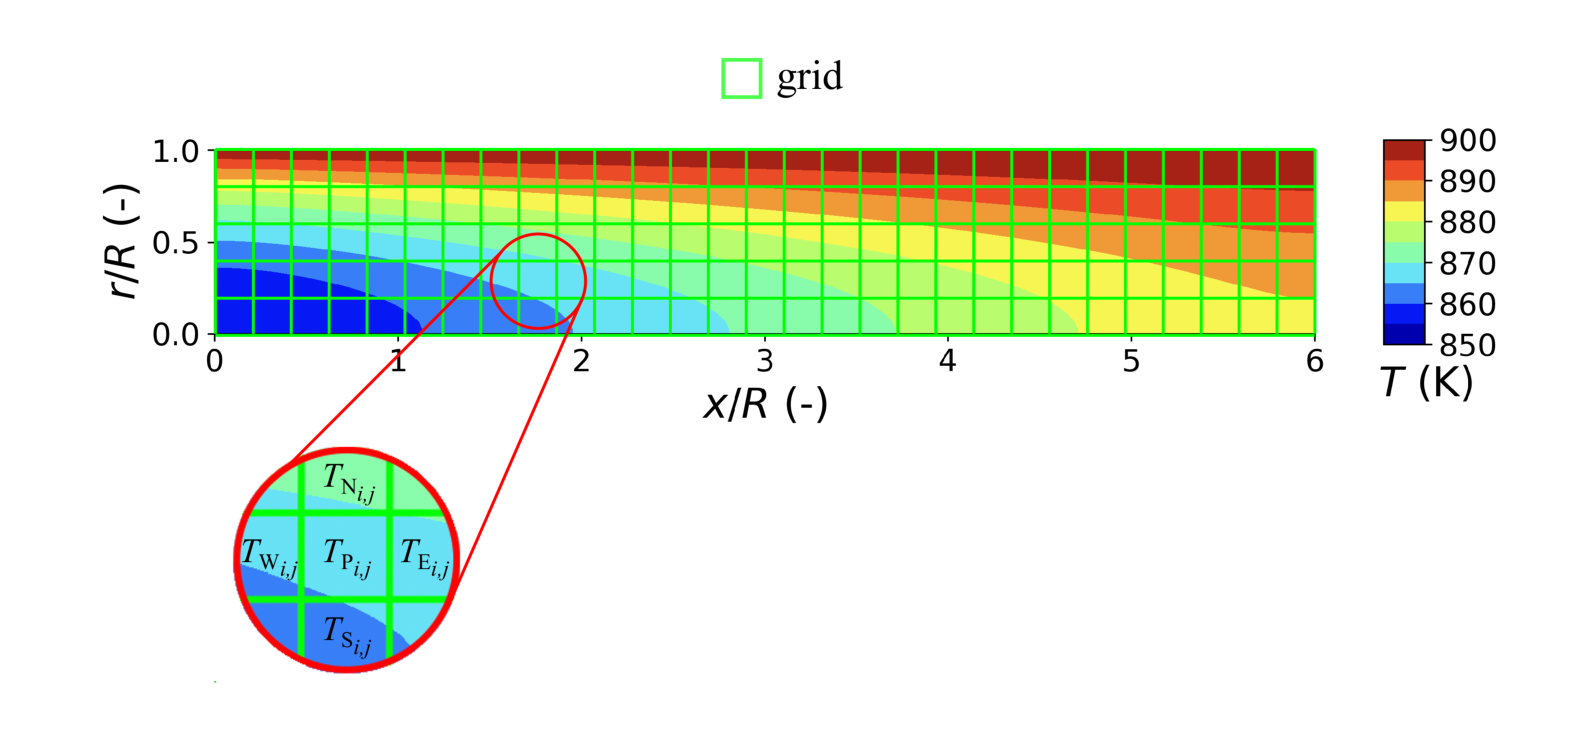
\includegraphics[width=130mm]{thermal_fitness.eps}\hspace{2pc}
\caption{\label{fig:f_T} Temperature field evaluation strategy}
\end{figure}

Having computed the set of the $\Delta T_{\rm{loc}_{\textit{i,j}}}$ for the whole numerical grid, the algorithm selects the highest value among computed $\Delta T_{{\rm{loc}}_{i,j}}$ and saves it as a global $\Delta T$ value representing a specific reactor (Eq. \eqref{eq:DT}).

\begin{equation}
\label{eq:DT}
\Delta T = {\rm{max}}\left\{ T_{{\rm{loc}}_{1,1}}, T_{{\rm{loc}}_{1,2}}, ... , T_{{\rm{loc}}_{i,j}}\right\},
\end{equation}

\noindent where $i$ and $j$ indices represent the numerical grid's dimensions. The final thermal fitness value $f_T$ is computed using the following formula: 

\begin{equation}
f_T = 1 - \frac{\Delta T}{\Delta T_{\rm{max}}},
\label{eq:T_fit}
\end{equation}

\noindent where $\Delta T_{\rm{max}}$ stands for the highest temperature difference value reported for a single generation. The acquired $f_{\rm{CH_4}}$ and $f_T$ values are further combined into a single fitness value $f$, using the weighted-sum method \cite{Zitzler1999}:

\begin{equation}
\label{eq:fitness}
f = \sum_{i = 1}^{N} w_{i}f_{i}.
\end{equation}

\noindent where $N$ represents the number of the specimens. The weights $w_{i}$ are established at 0.2, 0.4, 0.5, 0.6, and 0.8. Each of the analyses being carried out applied each of the weights to both of the fitness functions to allow the conduction of a sensitivity analysis, depending on the assumed importance of the defined fitness functions. The conducted numerical investigation includes a search for an optimal arrangement of coaxial segments, simultaneously performing a sensitivity analysis of the weights applied for the fitness calculation.

\clearpage








\section{Numerical analysis}
\label{sec:num_analysis}

The presented investigation regards the optimization of the temperature distribution inside the reforming reactor. Moderation of the temperature field is achieved via the introduction of the macro-patterning concept \cite{Pajak2018}. The concept predicts the modification of the catalytic insert of a reforming reactor, resulting in a change in the process conditions. The insert is divided into segments in the radial direction. Each segment may consist of catalytic Ni/YSZ or stainless steel foam. The algorithm conducts the search for an optimal composition of the insert, altering the percentage of the catalyst used, segments placement, and segments structural parameters.  The metallic foam is introduced to suppress the reforming reaction. A sensitivity analysis is conducted to specify the most suitable multiplication factors for the weighted-sum fitness calculation (Eq. \eqref{eq:fitness}) \cite{Davahli2022}. The computed fitness is used to rank the specimens in a single genetic algorithm's iteration. An analysis of the genetic algorithm behavior, depending on the weight applied to the two fitness functions is conducted, to define the most suitable approach to the issue, depending on the applied variant of the macro-patterning strategy. The analysis includes a comparison of results for five different sets of fitness weights, as follows:

\begin{itemize}
\item[1.] {$w_{\rm{CH_4}}  = 0.2$, $w_{T}  = 0.8$ }
\item[2.] {$w_{\rm{CH_4}}  = 0.4$, $w_{T}  = 0.6$ }
\item[3.] {$w_{\rm{CH_4}}  = 0.5$, $w_{T}  = 0.5$ }
\item[4.] {$w_{\rm{CH_4}}  = 0.6$, $w_{T}  = 0.4$ }
\item[5.] {$w_{\rm{CH_4}}  = 0.8$, $w_{T}  = 0.2$ }
\end{itemize}

The analysis has to be preceded by a definition of a reference case. A comparison of subsequent optimization results with the reference case will serve as a benchmark for defining if any significant improvement in the reaction conditions has been noted for a specific case. The reference case defined for the presented analysis is a conventional reforming reactor, with a catalytic insert being homogeneous and continuous throughout the whole volume of the reactor. The whole insert consists of a composite of nickel and yttrium-stabilized-zirconia (Ni/YSZ) with a ratio of 60:40. The porosity $\varepsilon$ of the reactor's catalyst is set at 50 \%, resulting in the catalyst density equal to 2.47 $\cdot$ 10$^6$ g m$^{-3}$. The average pore diameter $d_{\rm{p}}$ is established at 1.5 mm. The boundary conditions applied for the reference case are corresponding to the conditions set for the optimization procedure (Section \ref{sec:boundary}).

\begin{figure}[h]
\centering
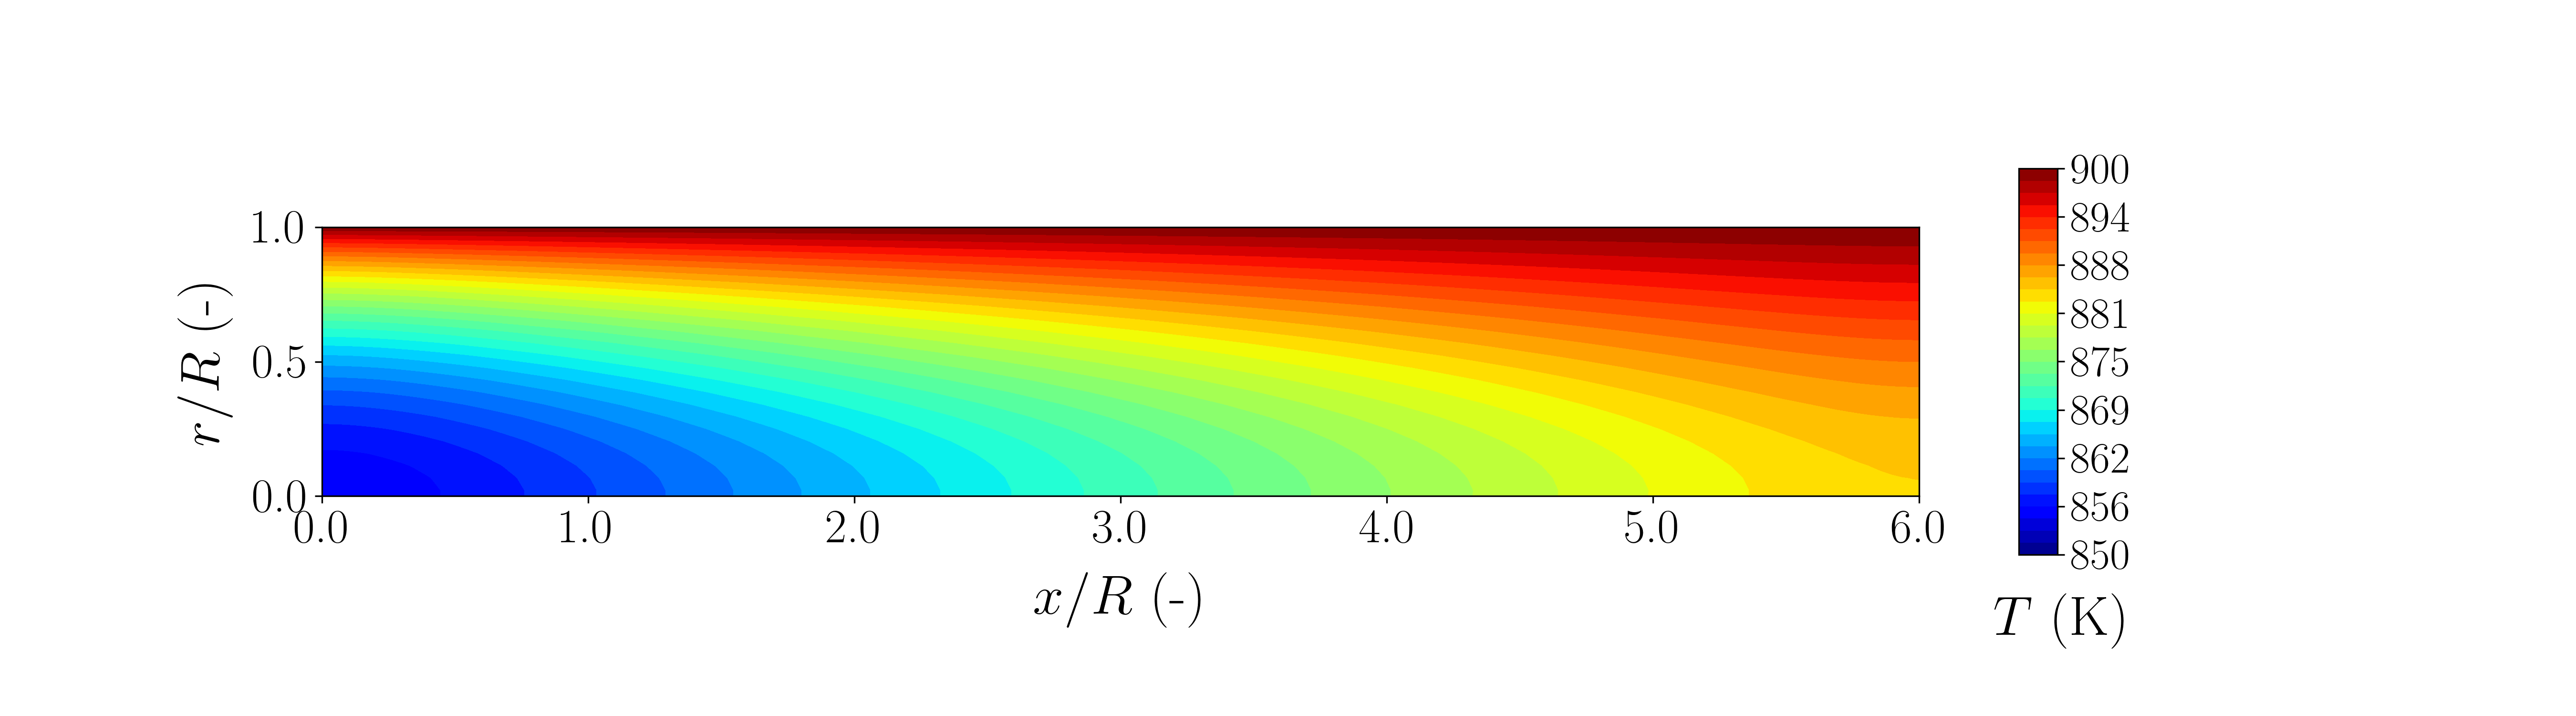
\includegraphics[width=190mm]{ref-Tfield.png}
\caption{\label{fig:ref-TField} Temperature field distribution - reference case ($T_{\rm{in}}$ = 900 K, $u_{\rm{in}}$ = 0.15 m s$^{-1}$, $SC$ = 2.0, $\dot{w}_{\rm{cat}}$ = 2.47 $\cdot$ 10$^{6}$)}
\end{figure}

The thermal characteristics of the reforming reaction in a conventional reactor can be observed in Fig. \ref{fig:ref-TField}). The reactor dimensions are divided by the reactor's radius (5 mm), to acquire a dimensionless set of coordinates. Observable temperature gradients are present throughout the whole volume of the reactor. The most significant temperature drop can be noticed at the inlet of the reactor, due to a considerable amount of energy required for the activation of the reforming reaction \cite{Xu1989, Pajak2018}. The molar fractions of specimens taking part in the process are illustrated in Fig. \ref{fig:ref-avg}. The molar fractions are averaged over the reactor's radius. Thus, the graph describes the change of the radius-averaged molar fractions in the longitudinal direction of the reactor. The values of the reactor's length are divided by the reactor's radius, to acquire dimensionless values.  

\begin{figure}[h]
\centering
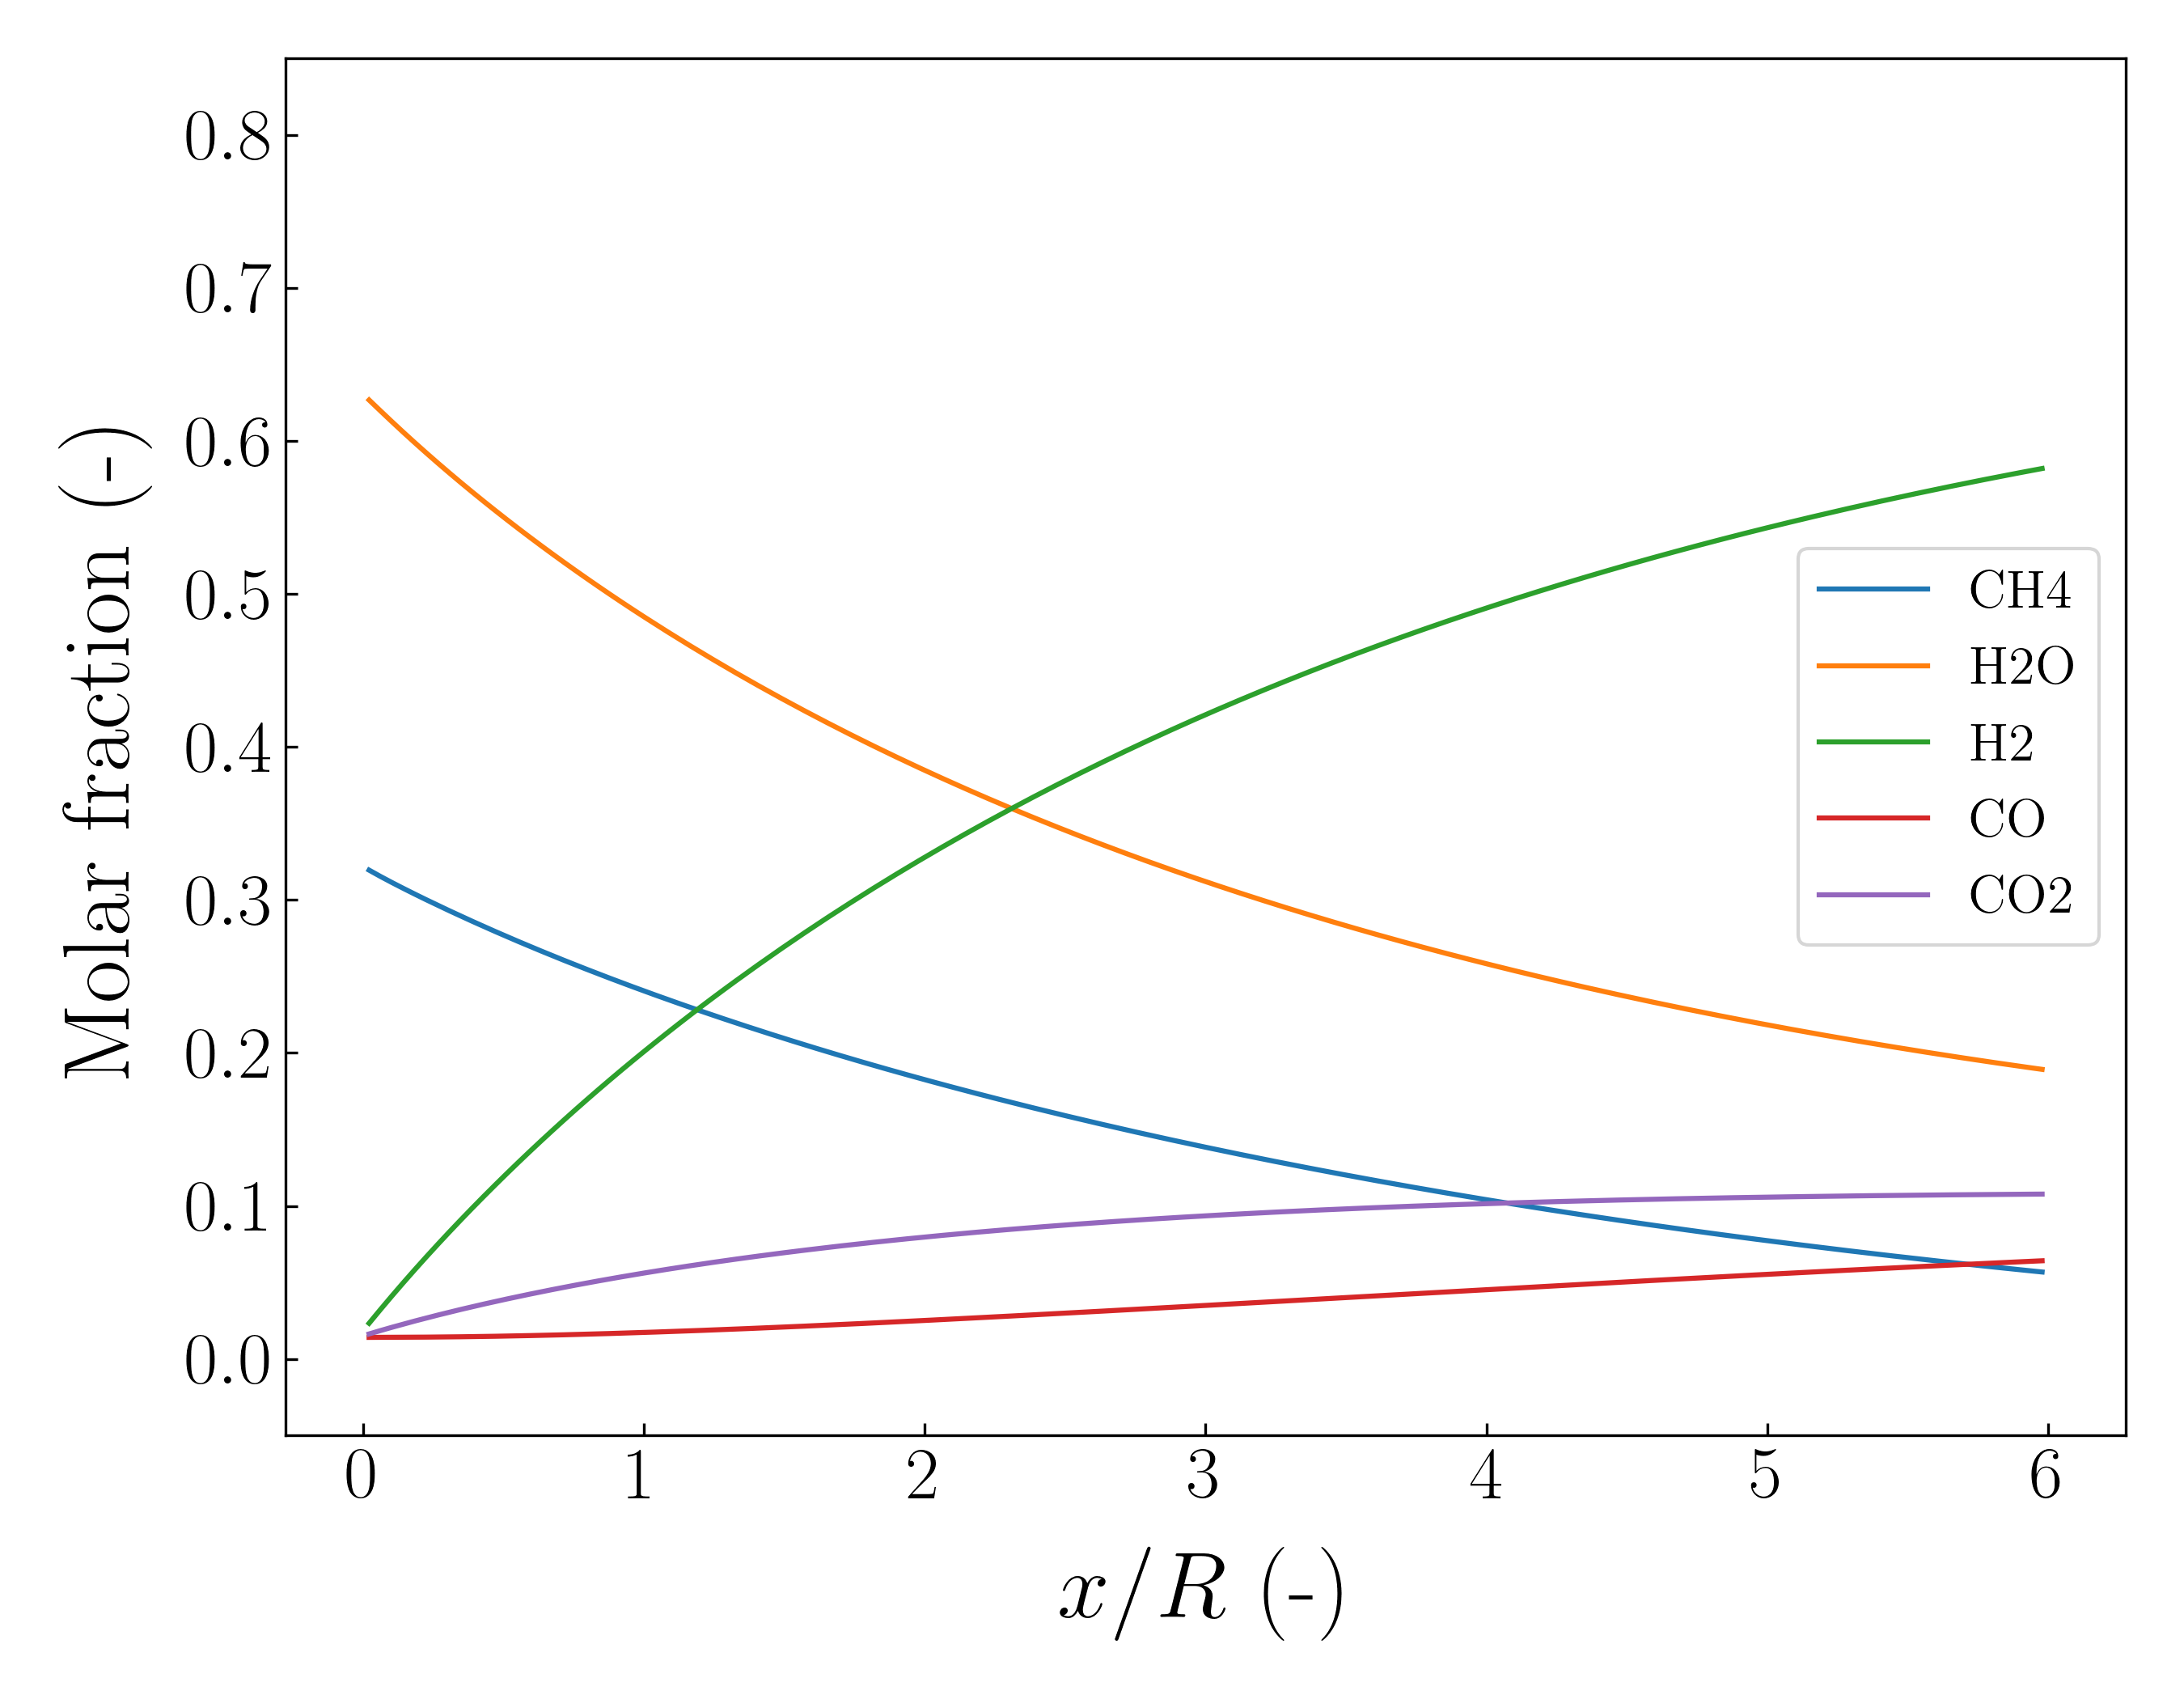
\includegraphics[width=100mm]{ref-avg.png}
\caption{\label{fig:ref-avg} Radius-averaged molar fractions - reference case ($T_{\rm{in}}$ = 900 K, $u_{\rm{in}}$ = 0.15 m s$^{-1}$, $SC$ = 2.0, $\dot{w}_{\rm{cat}}$ = 2.47 $\cdot$ 10$^{6}$)}
\end{figure}

The final stage of the numerical analysis predicted the extension of the macro-patterning concept by division of the catalytic insert in the radial direction, forming coaxial segments. The radial segments may accommodate one of two possible configurations. The first variant predicts cylinders with equal width of the inlet surface (Catalyst insert division strategy I), while the second introduces cylinders with an equal area of the inlet surfaces (Catalyst insert division strategy II) (Fig. \ref{fig:segments}). To allow a direct comparison between each of the composed algorithms, hydrogen productivity $\zeta$ is introduced. Hydrogen productivity delivers insight into the increase of the effectiveness of the reforming reaction for each of the optimized specimens. The $\zeta$ parameter is an exact ratio of the hydrogen output and the amount of the applied catalyst $\iota$  for a specific reactor (Eq. \eqref{eq:h2cat}).  The amount of the catalyst $\iota$ is calculated as the ratio of the catalyst used in a specific reactor, to the amount of the catalyst applied for the reference case.
 
 \begin{equation}
 \label{eq:h2cat}
 \zeta = \frac{\rm{H_{2_{out}}}}{\iota}
  \end{equation}

To deliver a comprehensive analysis of specific catalytic insert division strategies, a sensitivity analysis for each of them is conducted. The sensitivity analysis regards changing the weights $w_{\rm{CH_4}}$ and $w_T$ applied for specific fitness functions (Section \ref{chap:ga}).


\begin{figure}[h!]
\centering
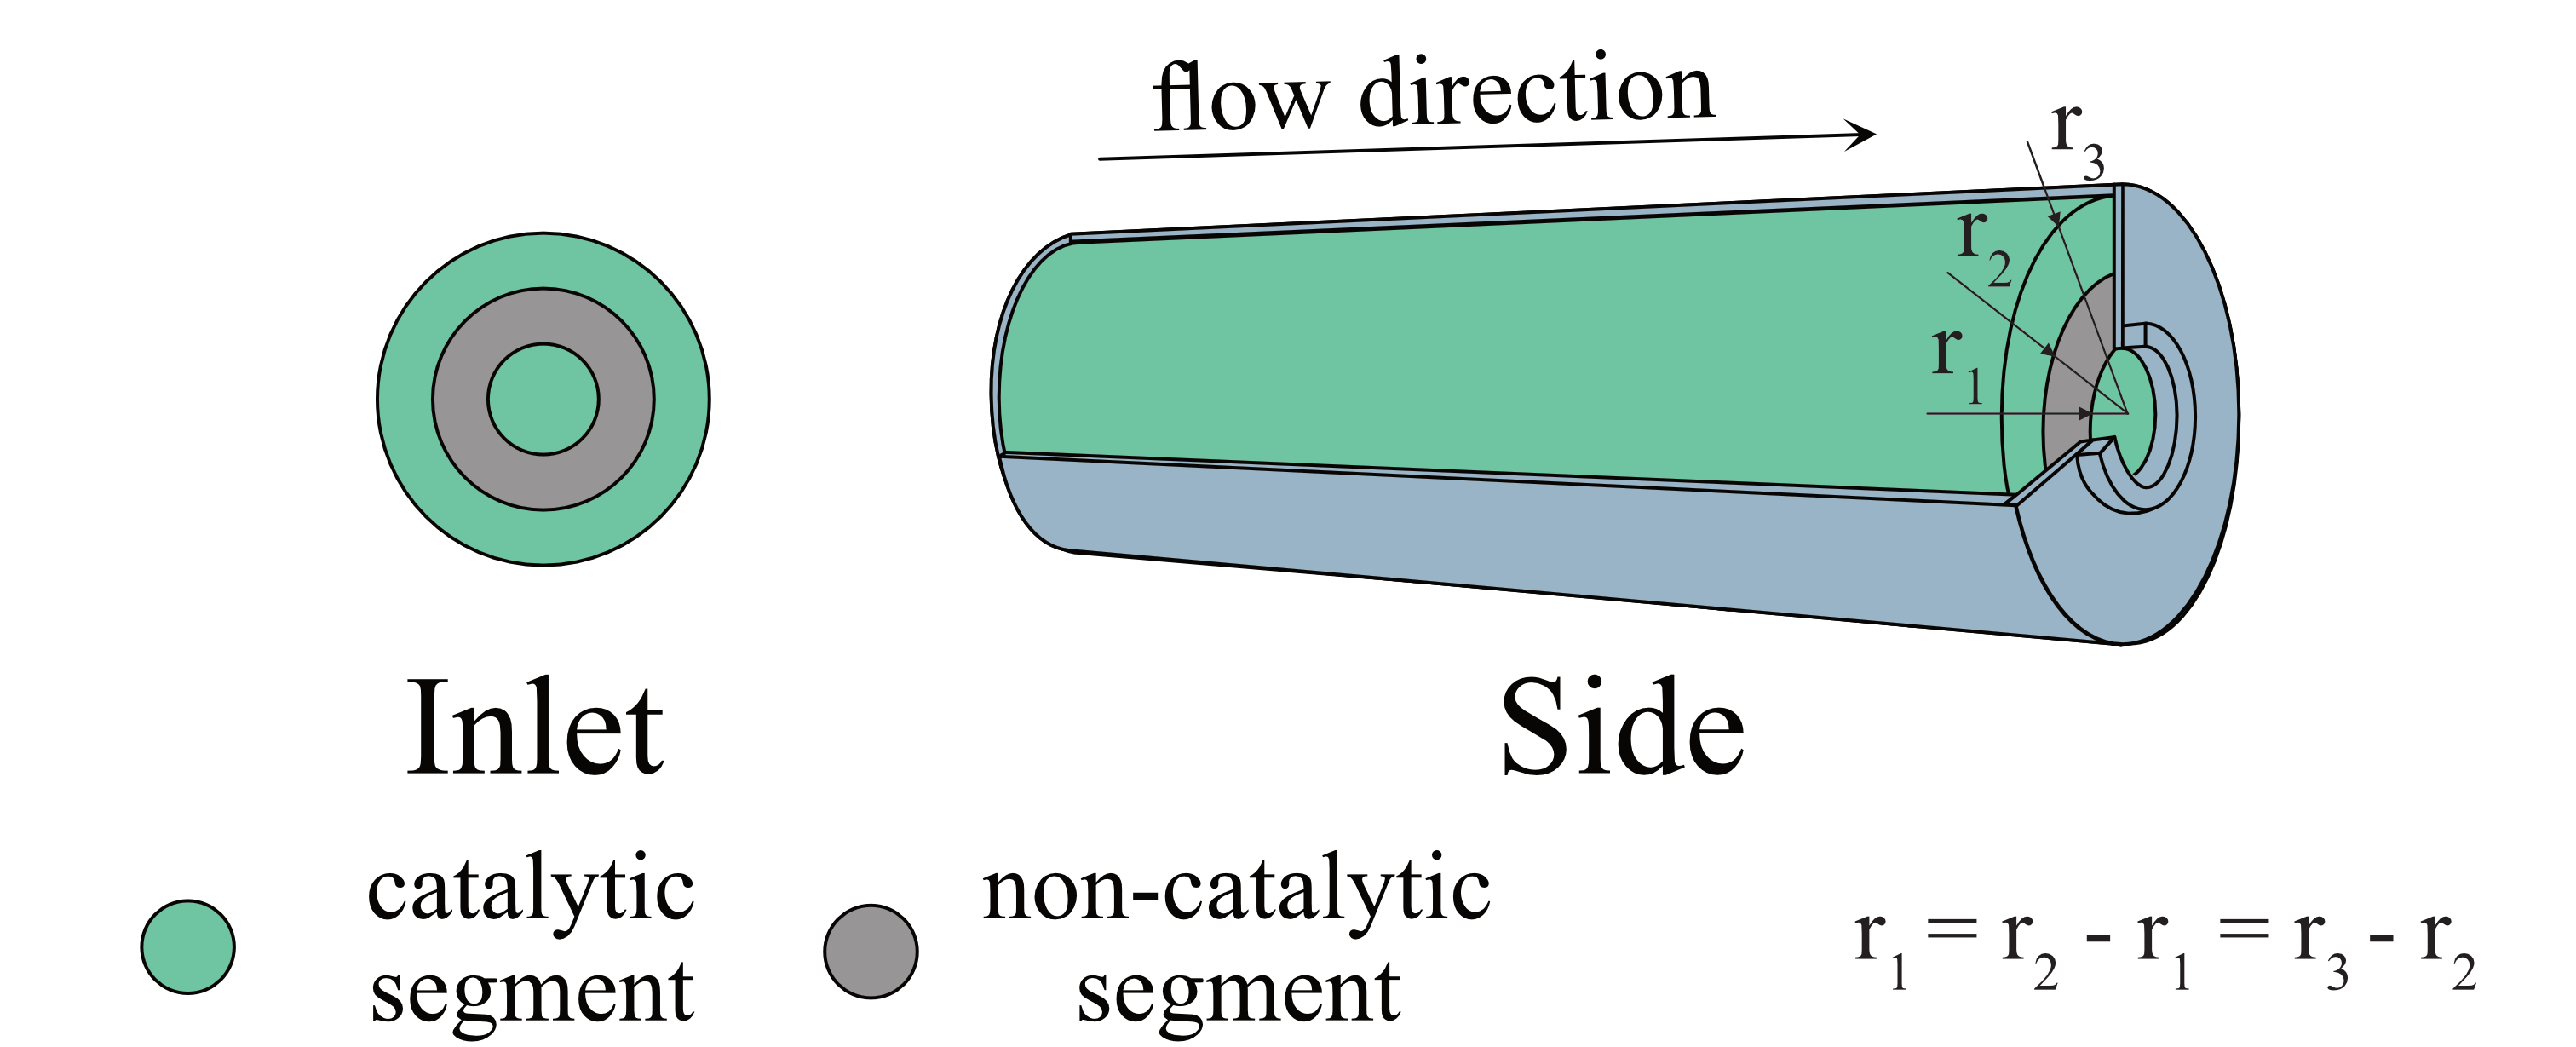
\includegraphics[width=120mm]{5seg.png}
\caption{\label{fig:5seg}Catalytic insert division strategy I}
\end{figure}


\paragraph{Thermal fitness 80 \%, methane conversion 20 \%} \hspace{0pt} \\
\noindent 

\begin{figure}[h!]
\centering
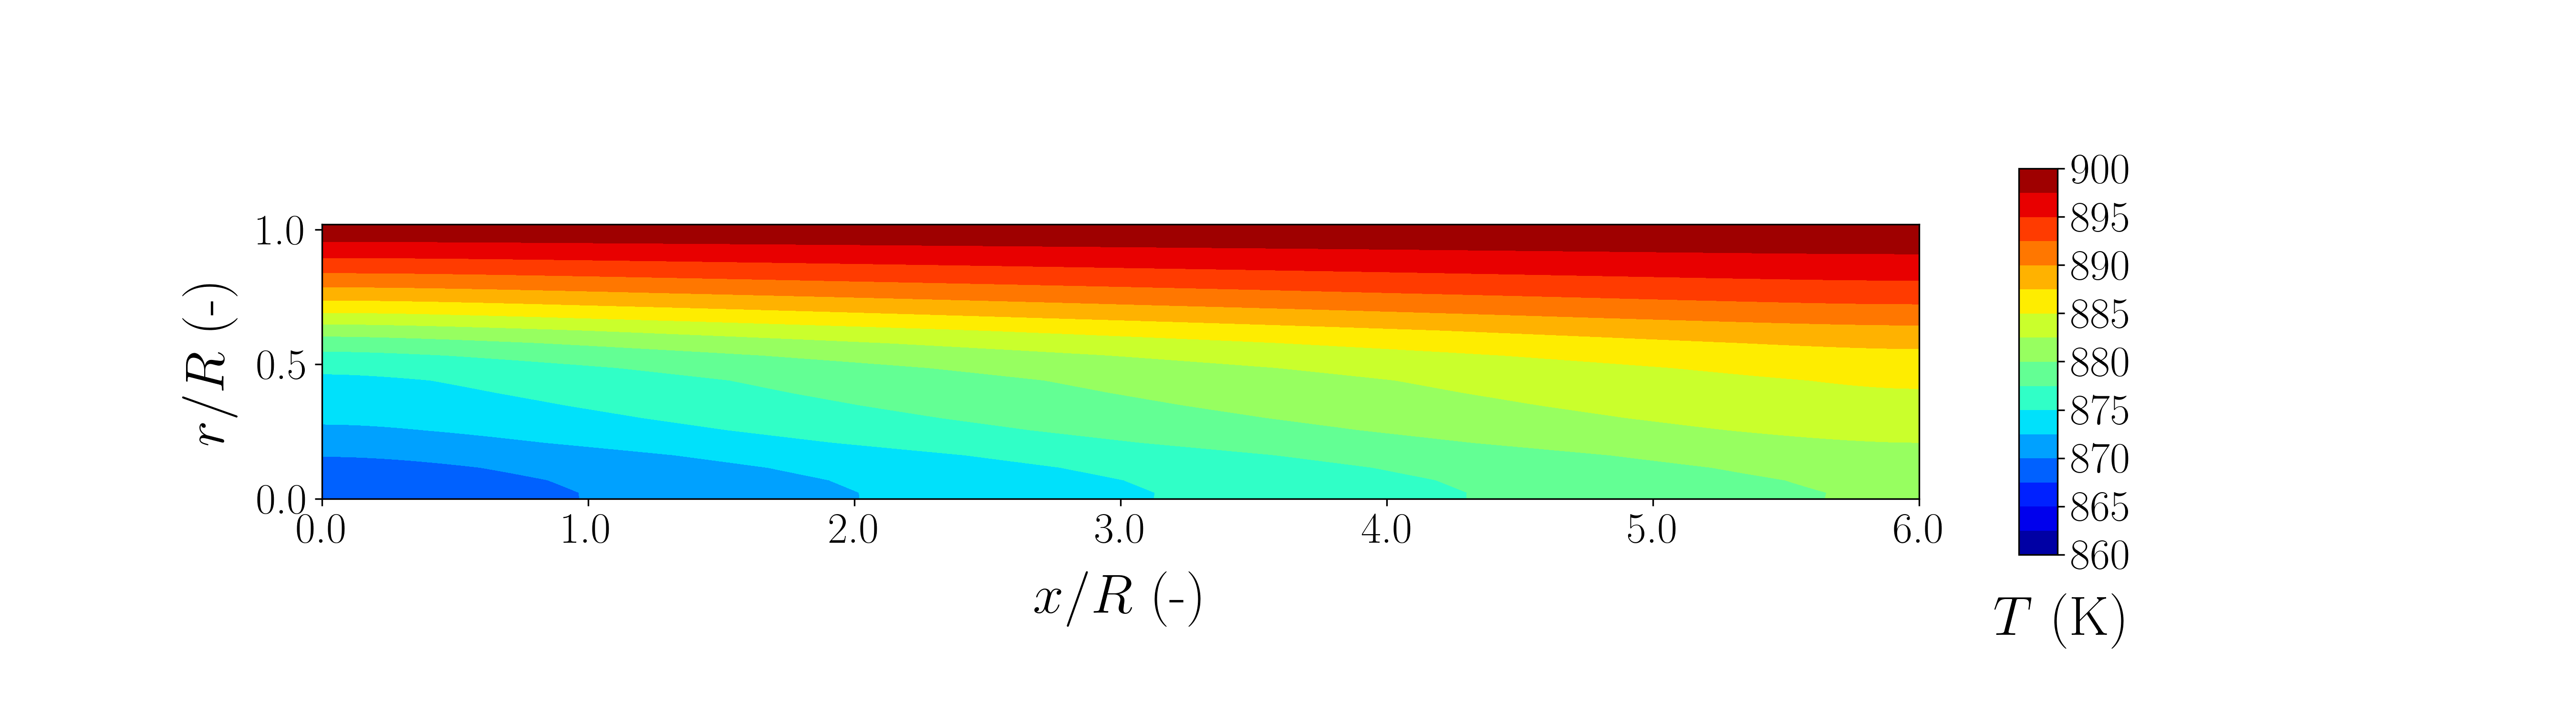
\includegraphics[width=190mm]{results/5/20C_80T/GEN1-TFIELD.png}
\caption{\label{fig:5R2080G1-TField} Strategy I - Temperature field distribution - 1$^{\rm{st}}$ generation ($w_{\rm{CH_4}} = 0.2, w_T = 0.8$, $T_{\rm{in}}$ = 900 K, $u_{\rm{in}}$ = 0.15 m s$^{-1}$, $SC$ = 2.0)}
\end{figure}

\begin{figure}[h!]
\centering
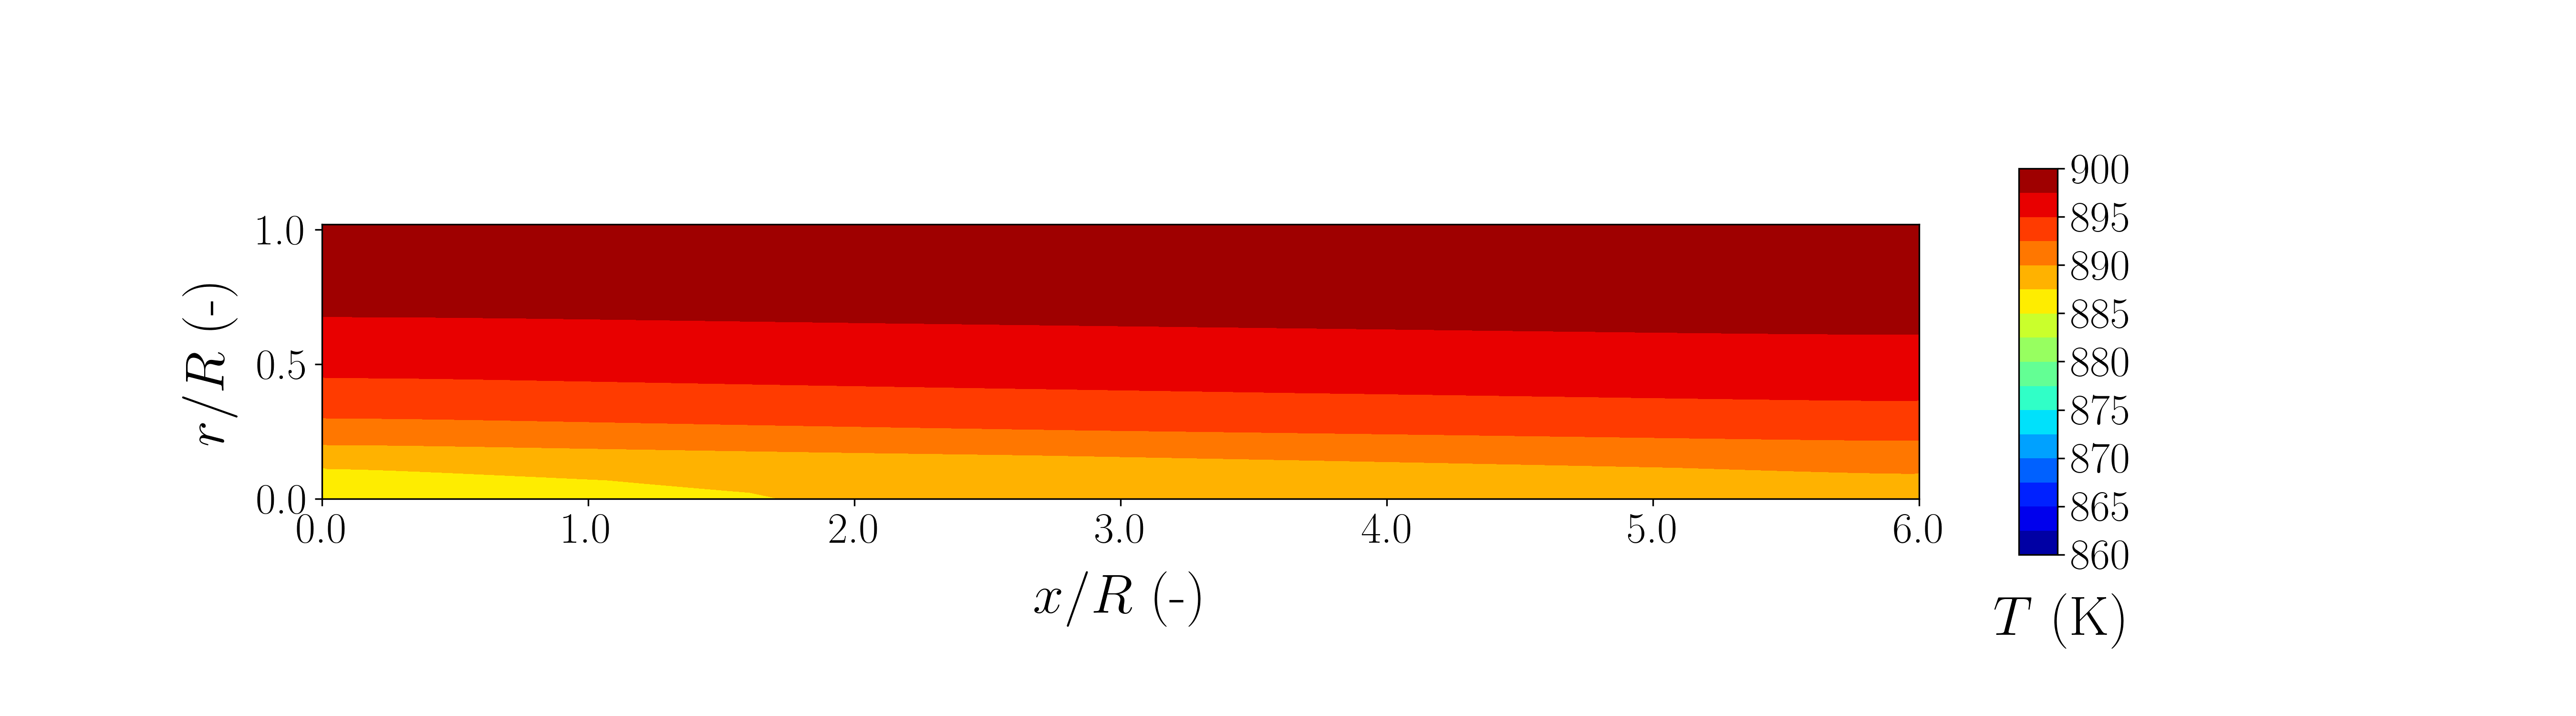
\includegraphics[width=190mm]{results/5/20C_80T/GEN15-TFIELD.png}
\caption{\label{fig:5R2080G15-TField} Strategy I - Temperature field distribution - 15$^{\rm{th}}$ generation ($w_{\rm{CH_4}} = 0.2, w_T = 0.8$, $T_{\rm{in}}$ = 900 K, $u_{\rm{in}}$ = 0.15 m s$^{-1}$, $SC$ = 2.0)}
\end{figure}

\begin{figure}[h!]
\centering
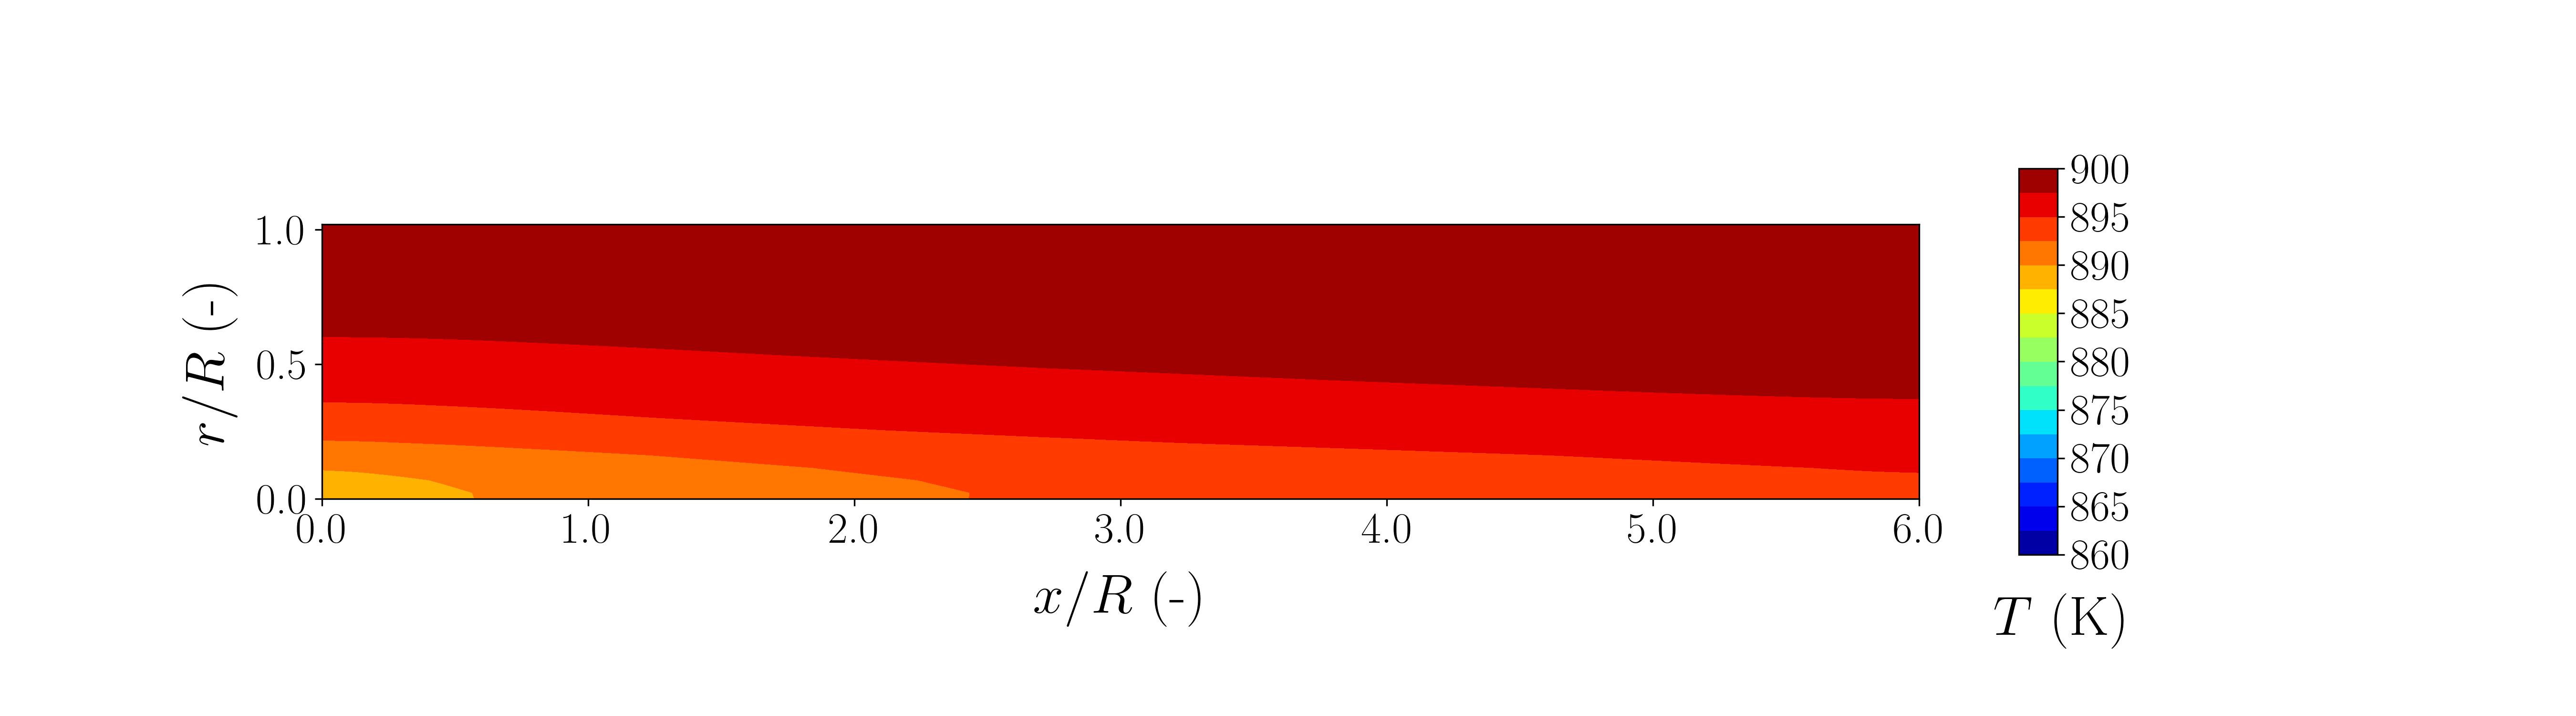
\includegraphics[width=190mm]{results/5/20C_80T/GEN30-TFIELD.png}
\caption{\label{fig:5R2080G30-TField} Strategy I - Temperature field distribution - 30$^{\rm{th}}$ generation ($w_{\rm{CH_4}} = 0.2, w_T = 0.8$, $T_{\rm{in}}$ = 900 K, $u_{\rm{in}}$ = 0.15 m s$^{-1}$, $SC$ = 2.0)}
\end{figure}


\begin{figure}[h!]
\centering
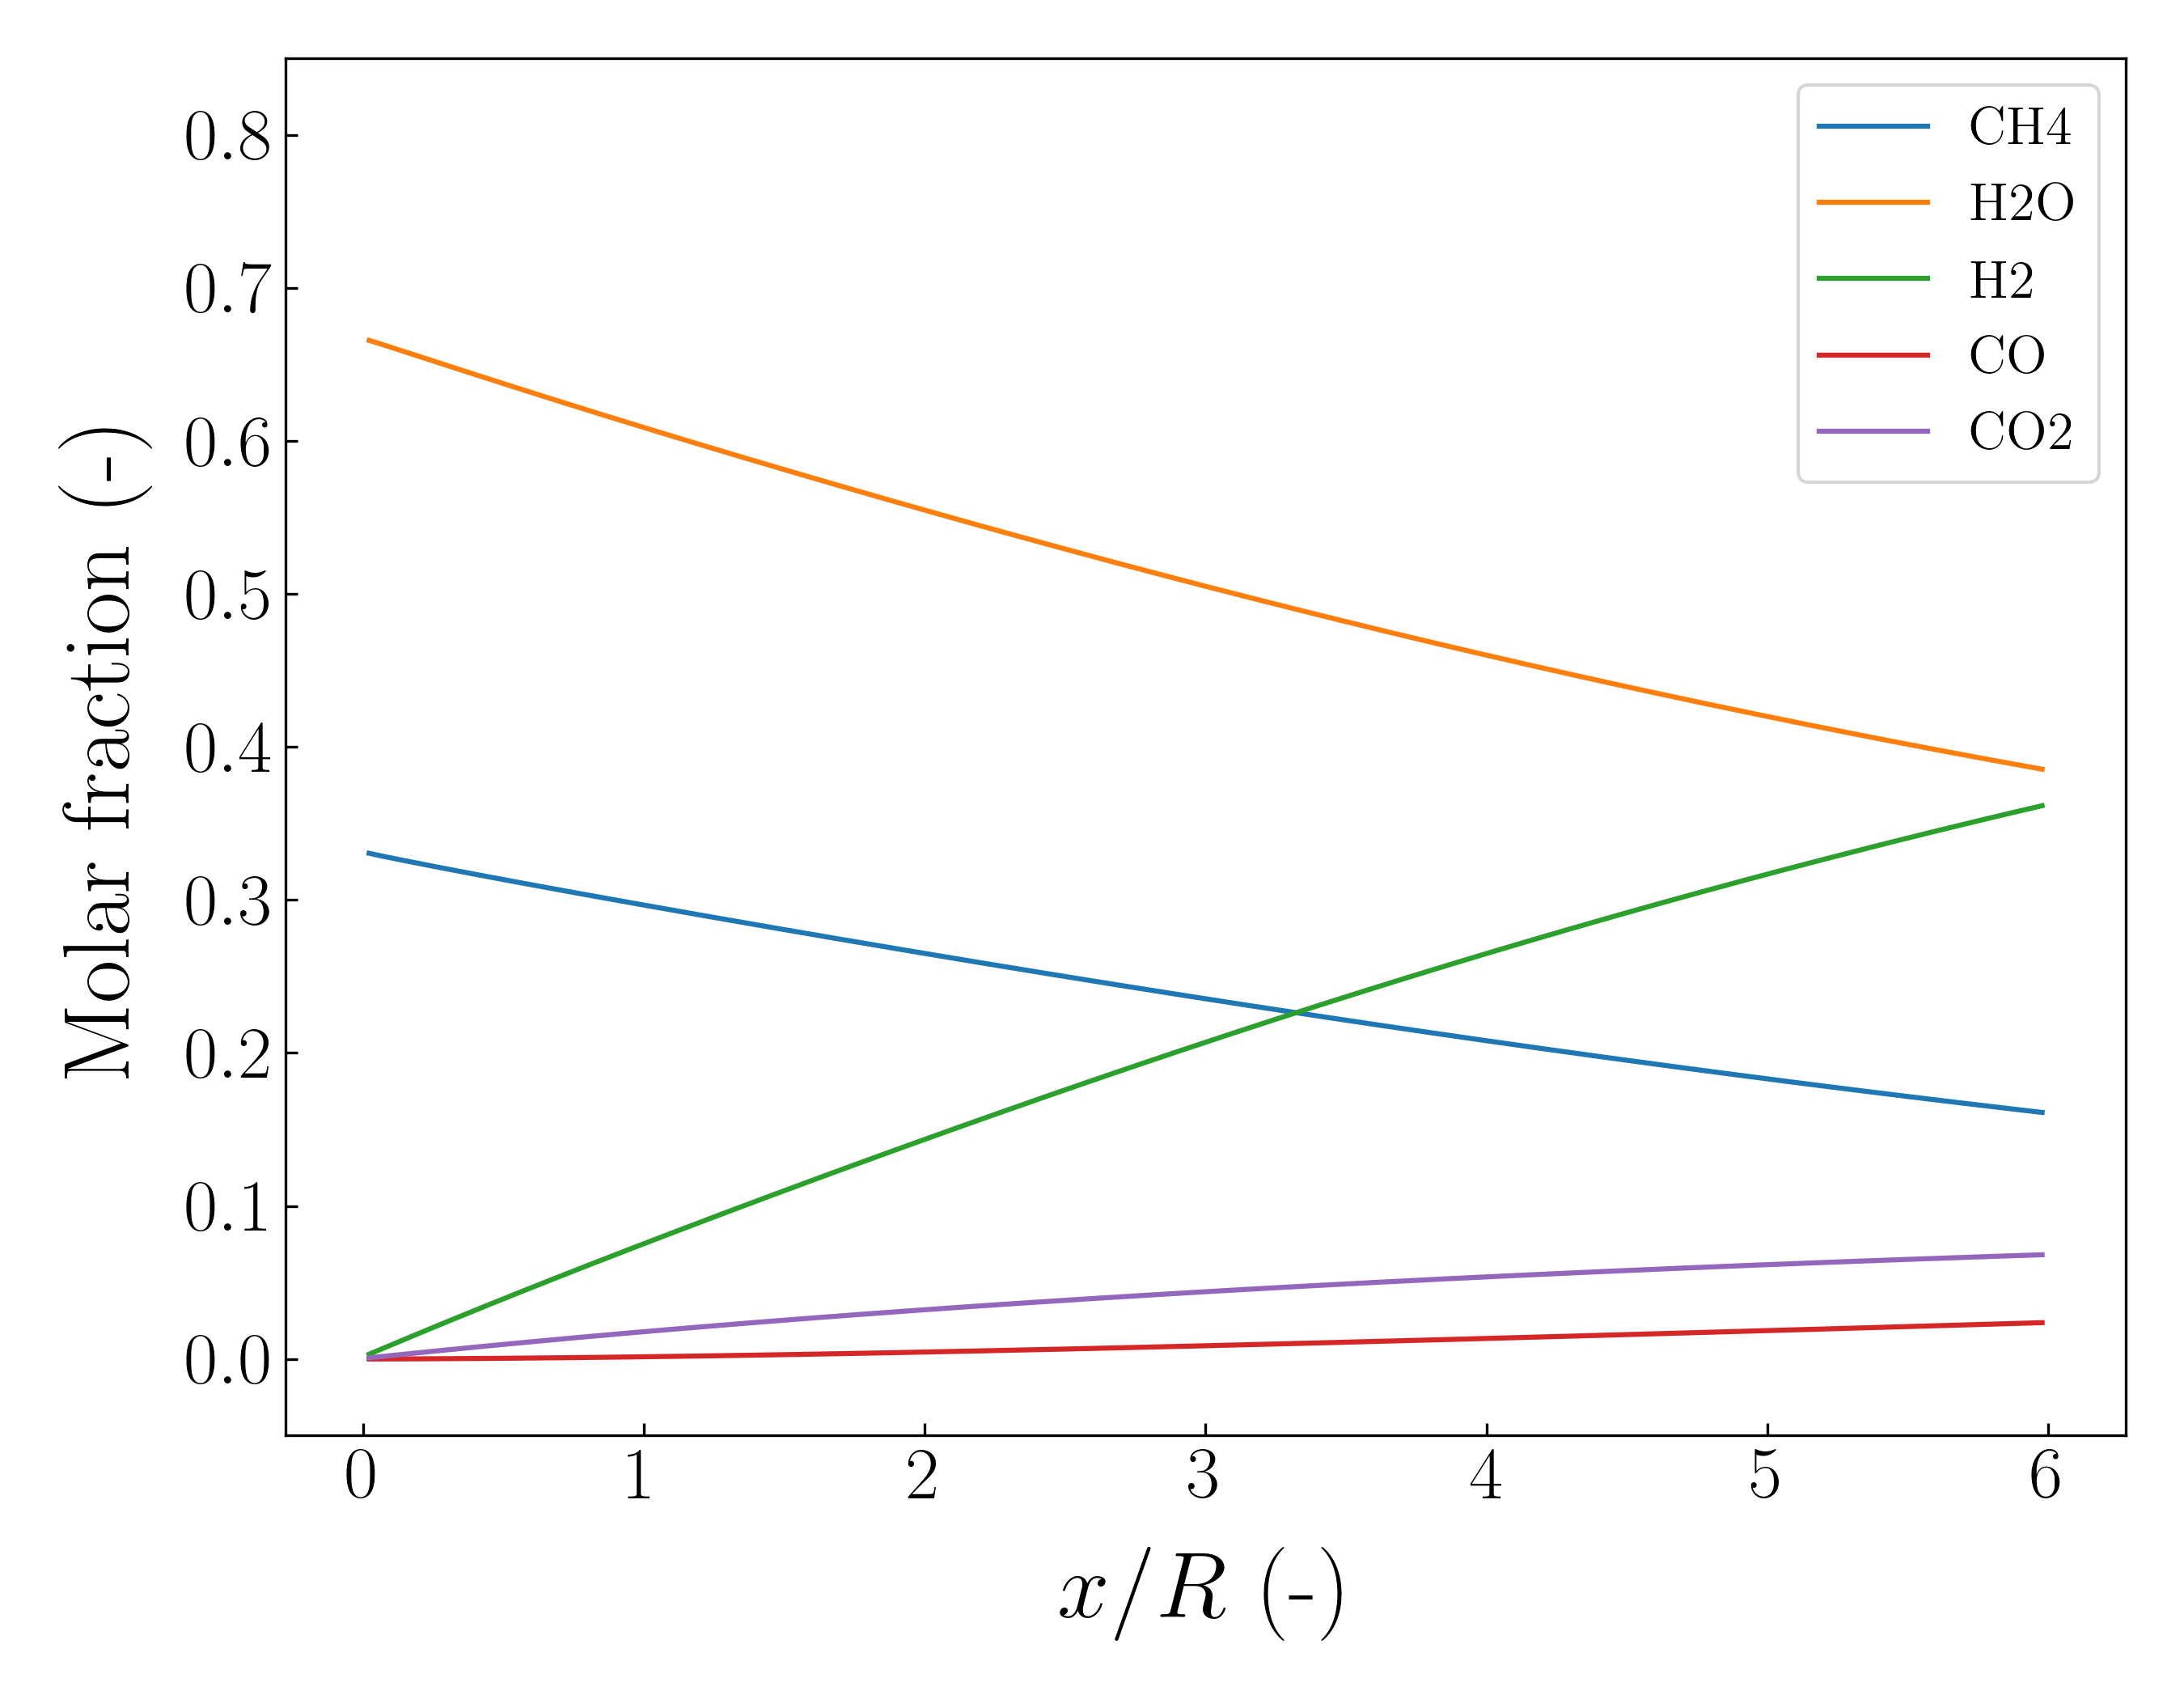
\includegraphics[width=80mm]{results/5/20C_80T/GEN1-AVG.png}
\caption{\label{fig:5R2080G1-avg} Strategy I - Radius-averaged molar fractions - 1$^{\rm{st}}$ generation ($w_{\rm{CH_4}} = 0.2, w_T = 0.8$, $T_{\rm{in}}$ = 900 K, $u_{\rm{in}}$ = 0.15 m s$^{-1}$, $SC$ = 2.0)}
\end{figure}

\begin{figure}[h!]
\centering
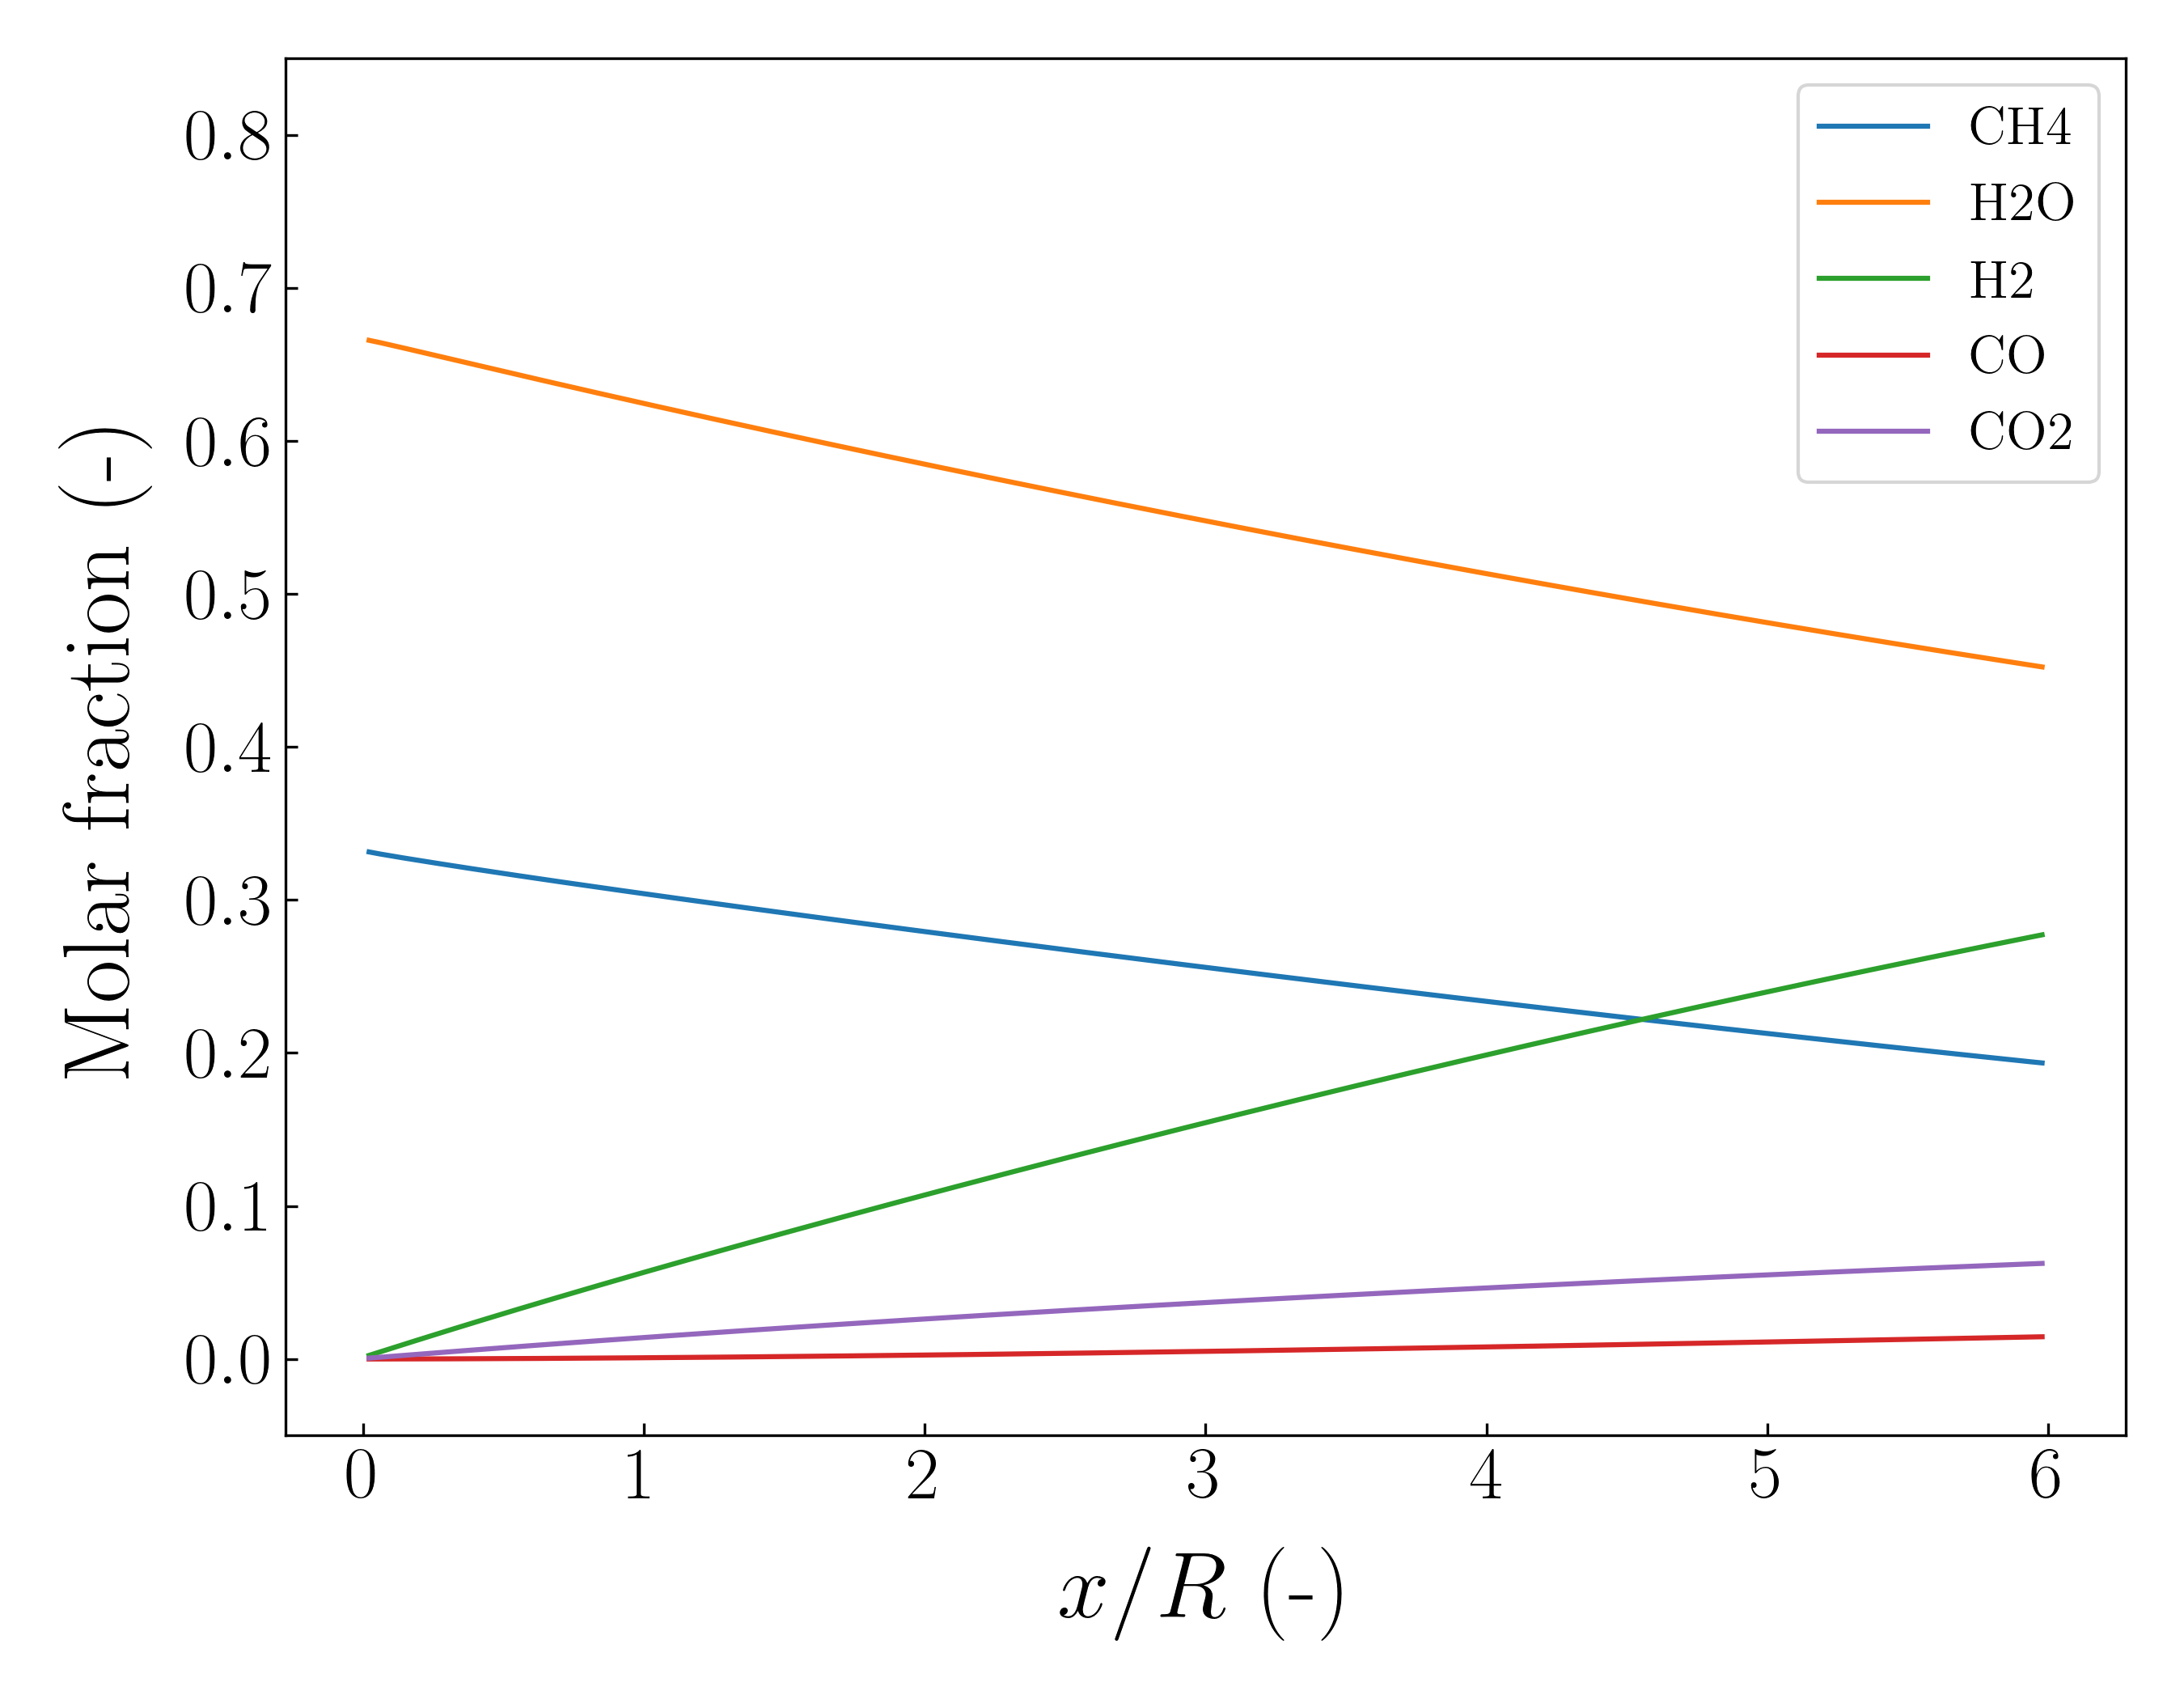
\includegraphics[width=80mm]{results/5/20C_80T/GEN15-AVG.png}
\caption{\label{fig:5R2080G15-avg} Strategy I - Radius-averaged molar fractions - 15$^{\rm{th}}$ generation ($w_{\rm{CH_4}} = 0.2, w_T = 0.8$, $T_{\rm{in}}$ = 900 K, $u_{\rm{in}}$ = 0.15 m s$^{-1}$, $SC$ = 2.0)}
\end{figure}

\begin{figure}[h!]
\centering
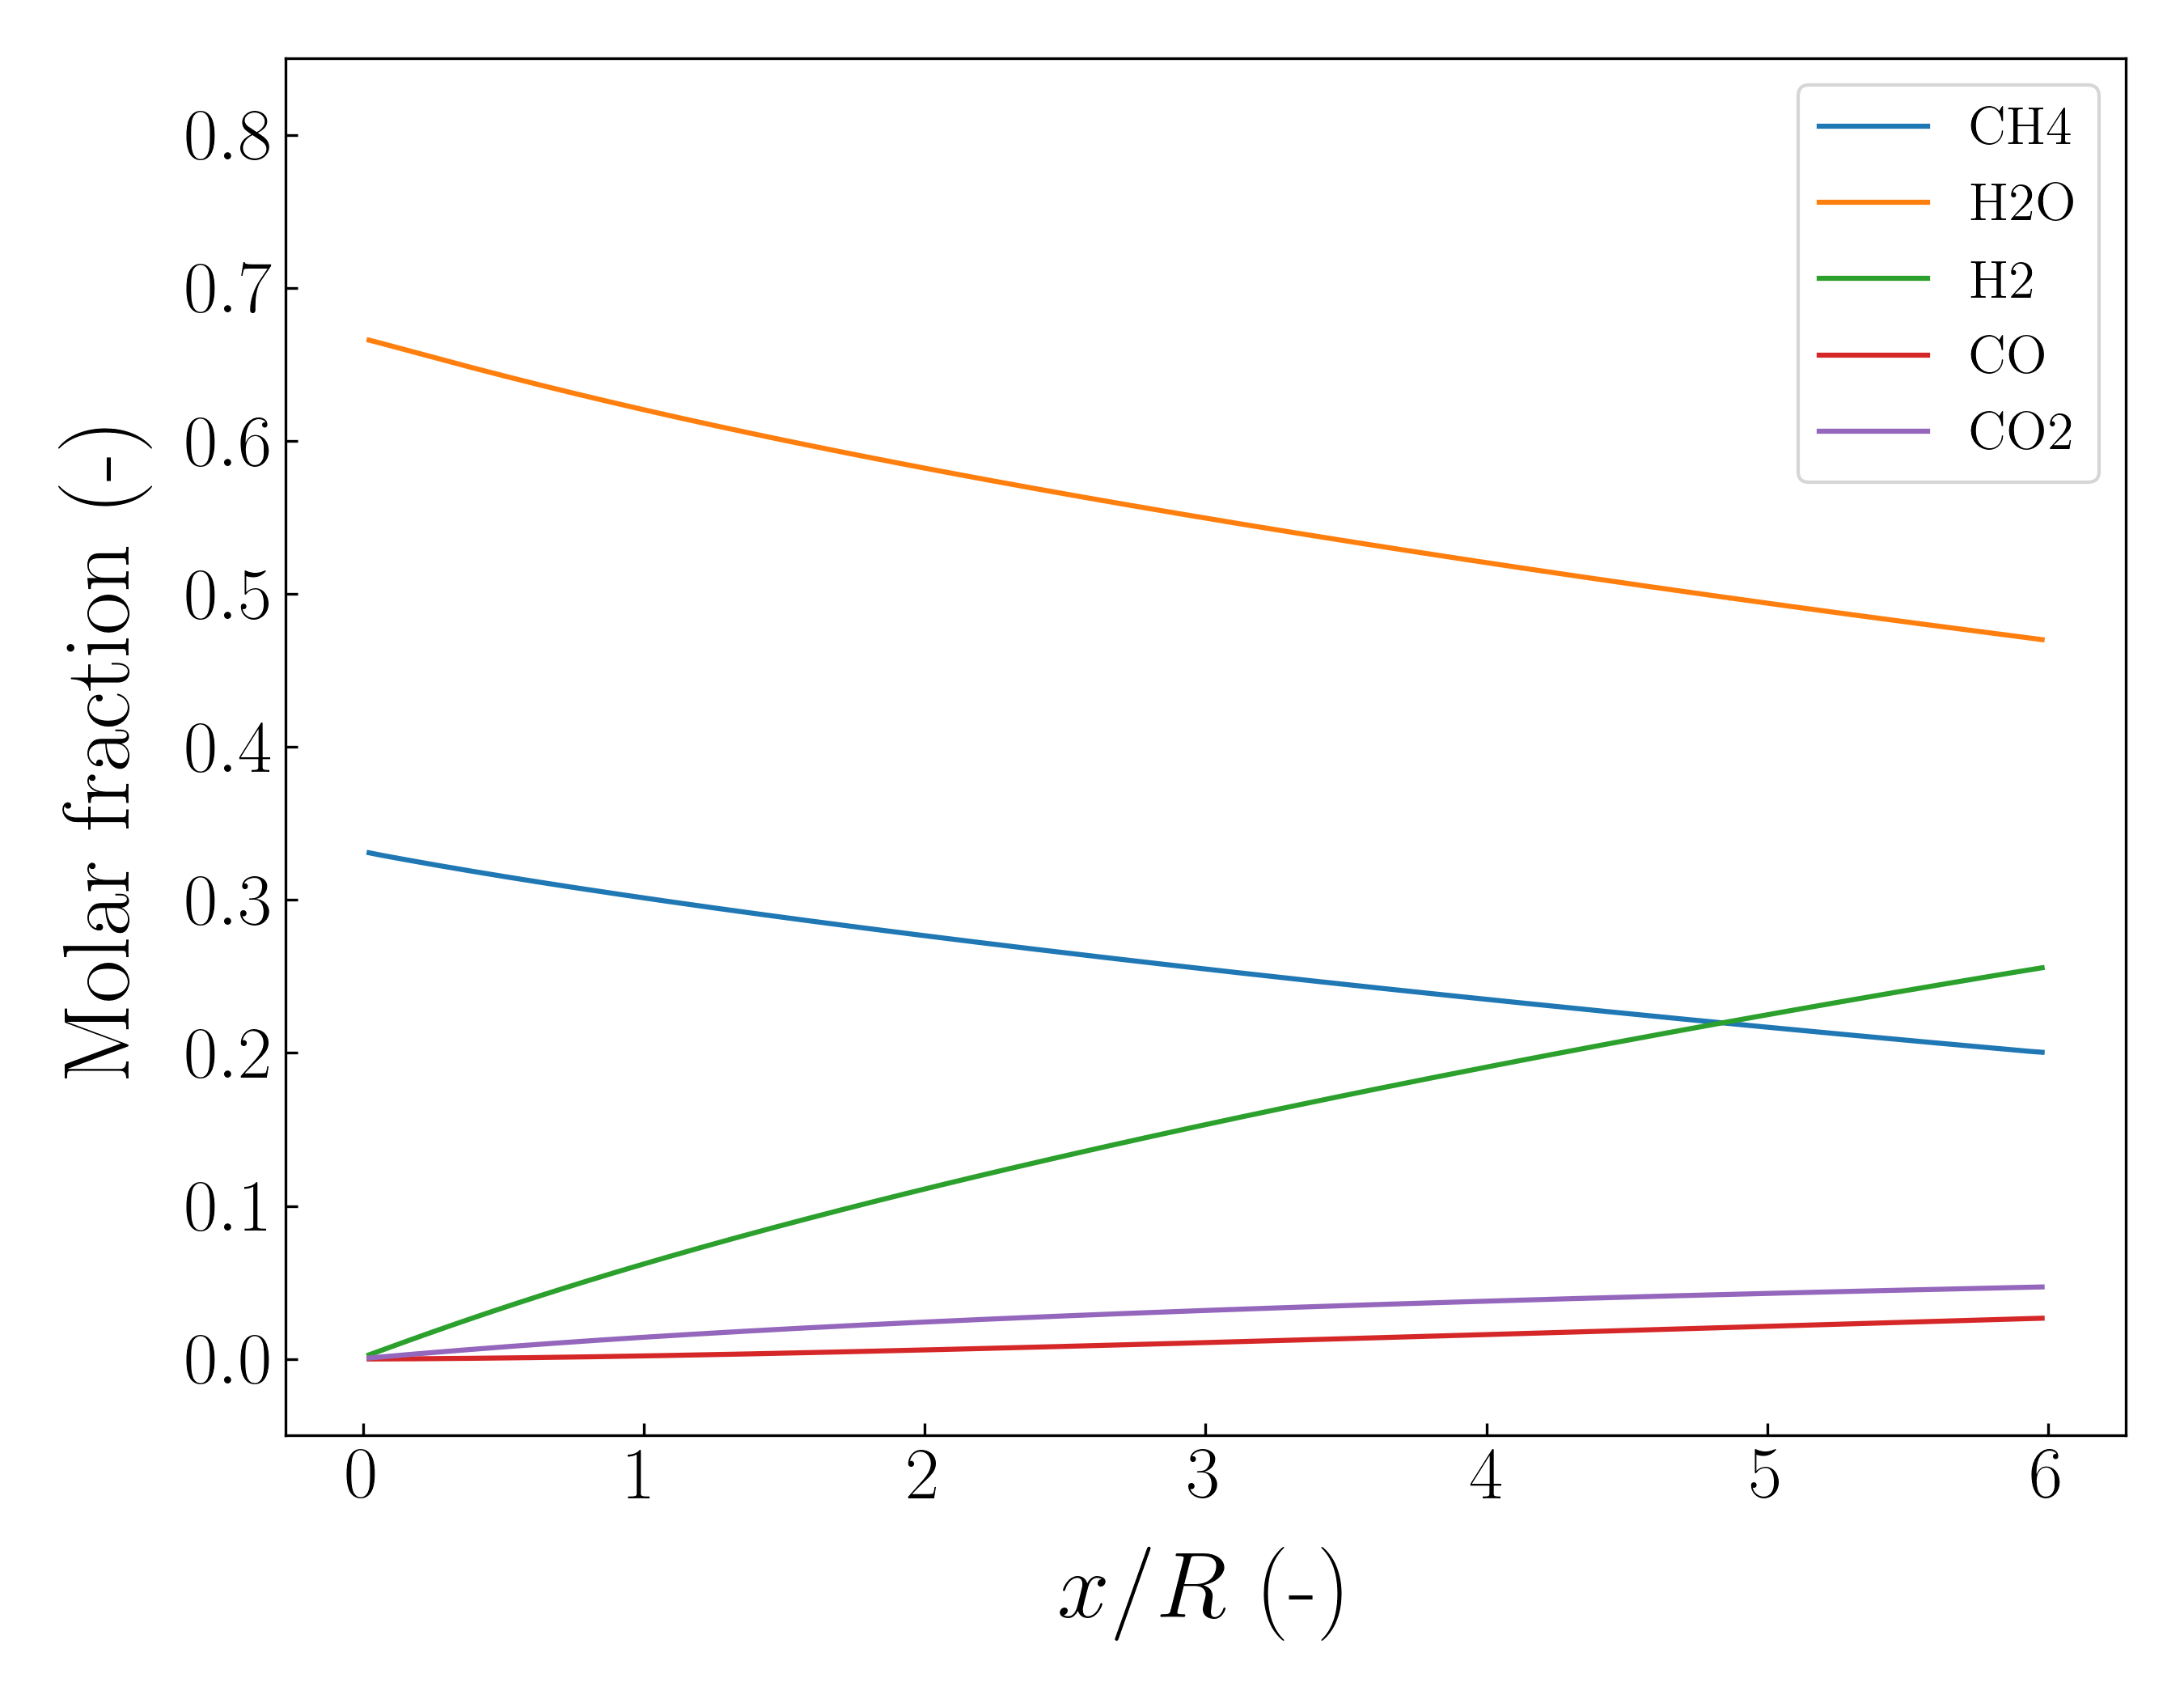
\includegraphics[width=80mm]{results/5/20C_80T/GEN30-AVG.png}
\caption{\label{fig:5R2080G30-avg} Strategy I - Radius-averaged molar fractions -  30$^{\rm{th}}$ generation ($w_{\rm{CH_4}} = 0.2, w_T = 0.8$, $T_{\rm{in}}$ = 900 K, $u_{\rm{in}}$ = 0.15 m s$^{-1}$, $SC$ = 2.0)}
\end{figure}

\begin{figure}[h!]
\centering
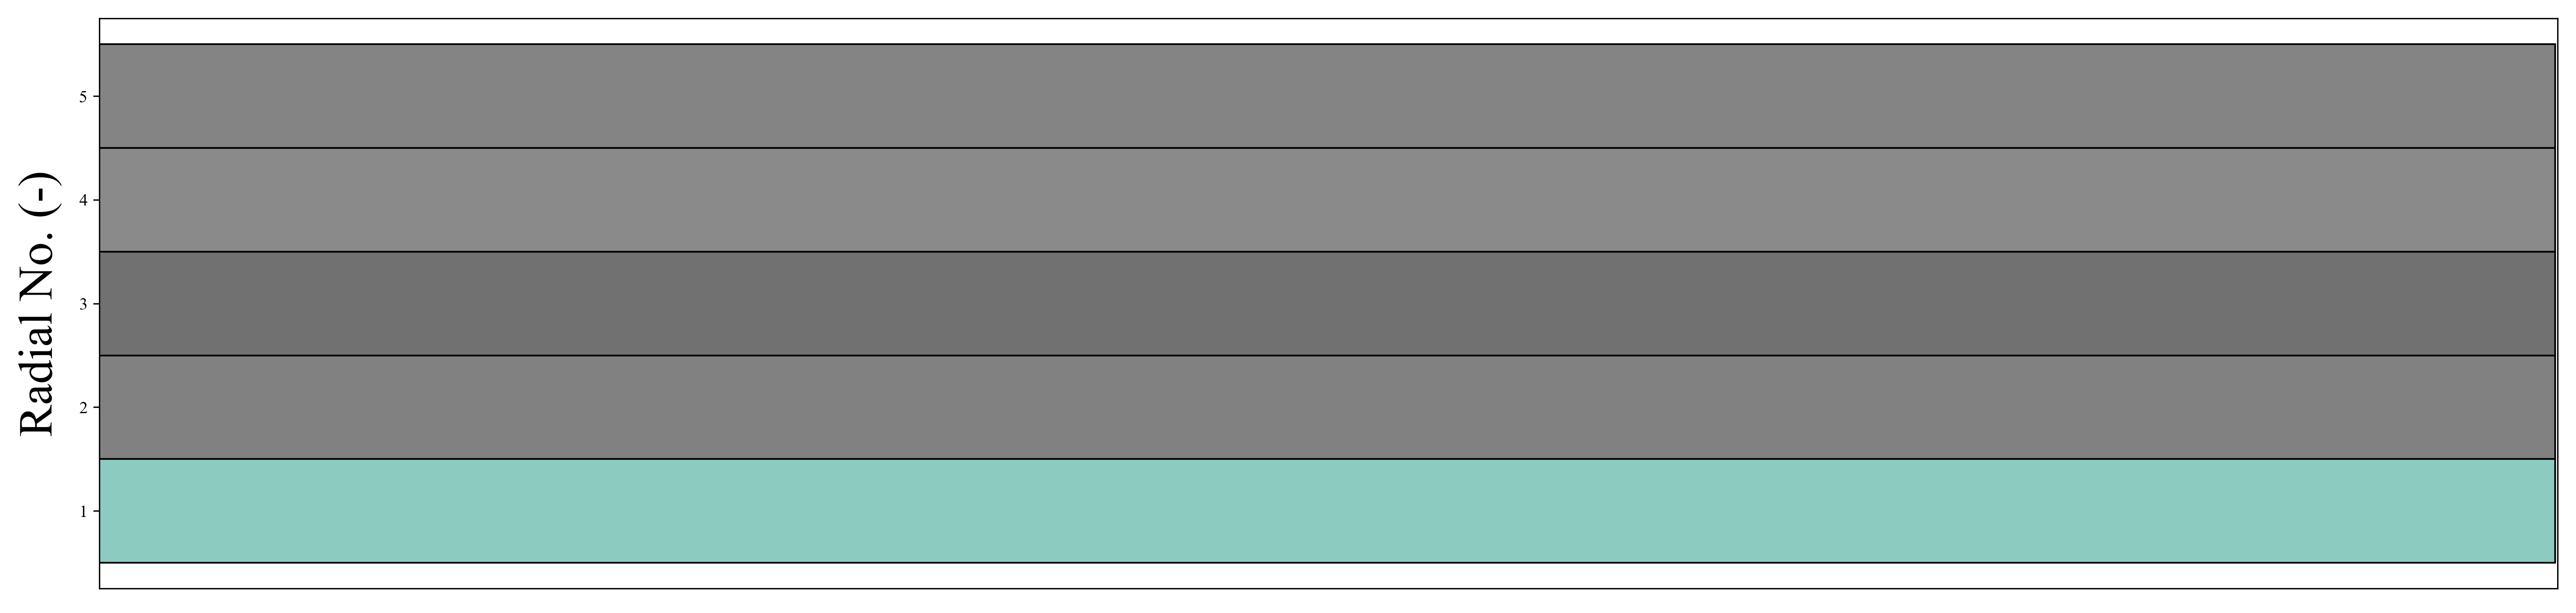
\includegraphics[width=120mm]{results/segments/5seg/20C80T/seg.png}
\caption{\label{fig:30L6040G1-TField} Strategy I - Segments distribution for 30$^{\rm{th}}$ generation ($w_{\rm{CH_4}} = 0.2, w_T = 0.8$, $T_{\rm{in}}$ = 900 K, $u_{\rm{in}}$ = 0.15 m s$^{-1}$, $SC$ = 2.0)}
\end{figure}

%\begin{figure}[h!]
%\centering
%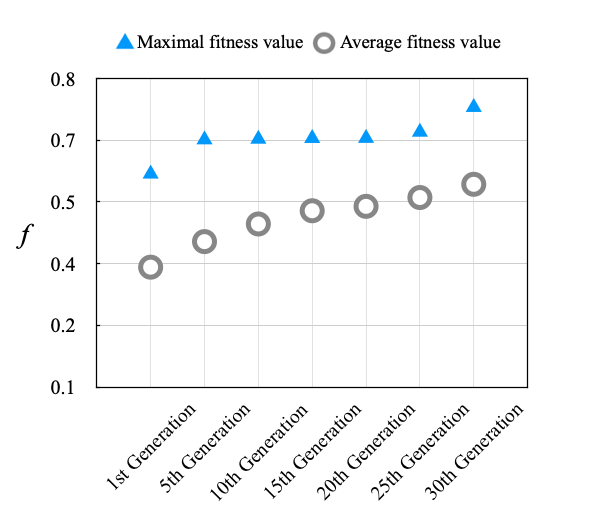
\includegraphics[width=100mm]{results/5/20C_80T.png}
%\caption{\label{fig:5R2080G-fitness} Strategy I - Fitness analysis throughout successive populations ($w_{\rm{CH_4}} = 0.2, w_T = 0.8$, $T_{\rm{in}}$ = 900 K, $u_{\rm{in}}$ = 0.15 m s$^{-1}$, $SC$ = 2.0)}
%\end{figure}



\clearpage



\paragraph{Thermal fitness 60 \%, methane conversion 40 \%} \hspace{0pt} \\
\noindent 


\begin{figure}[h!]
\centering
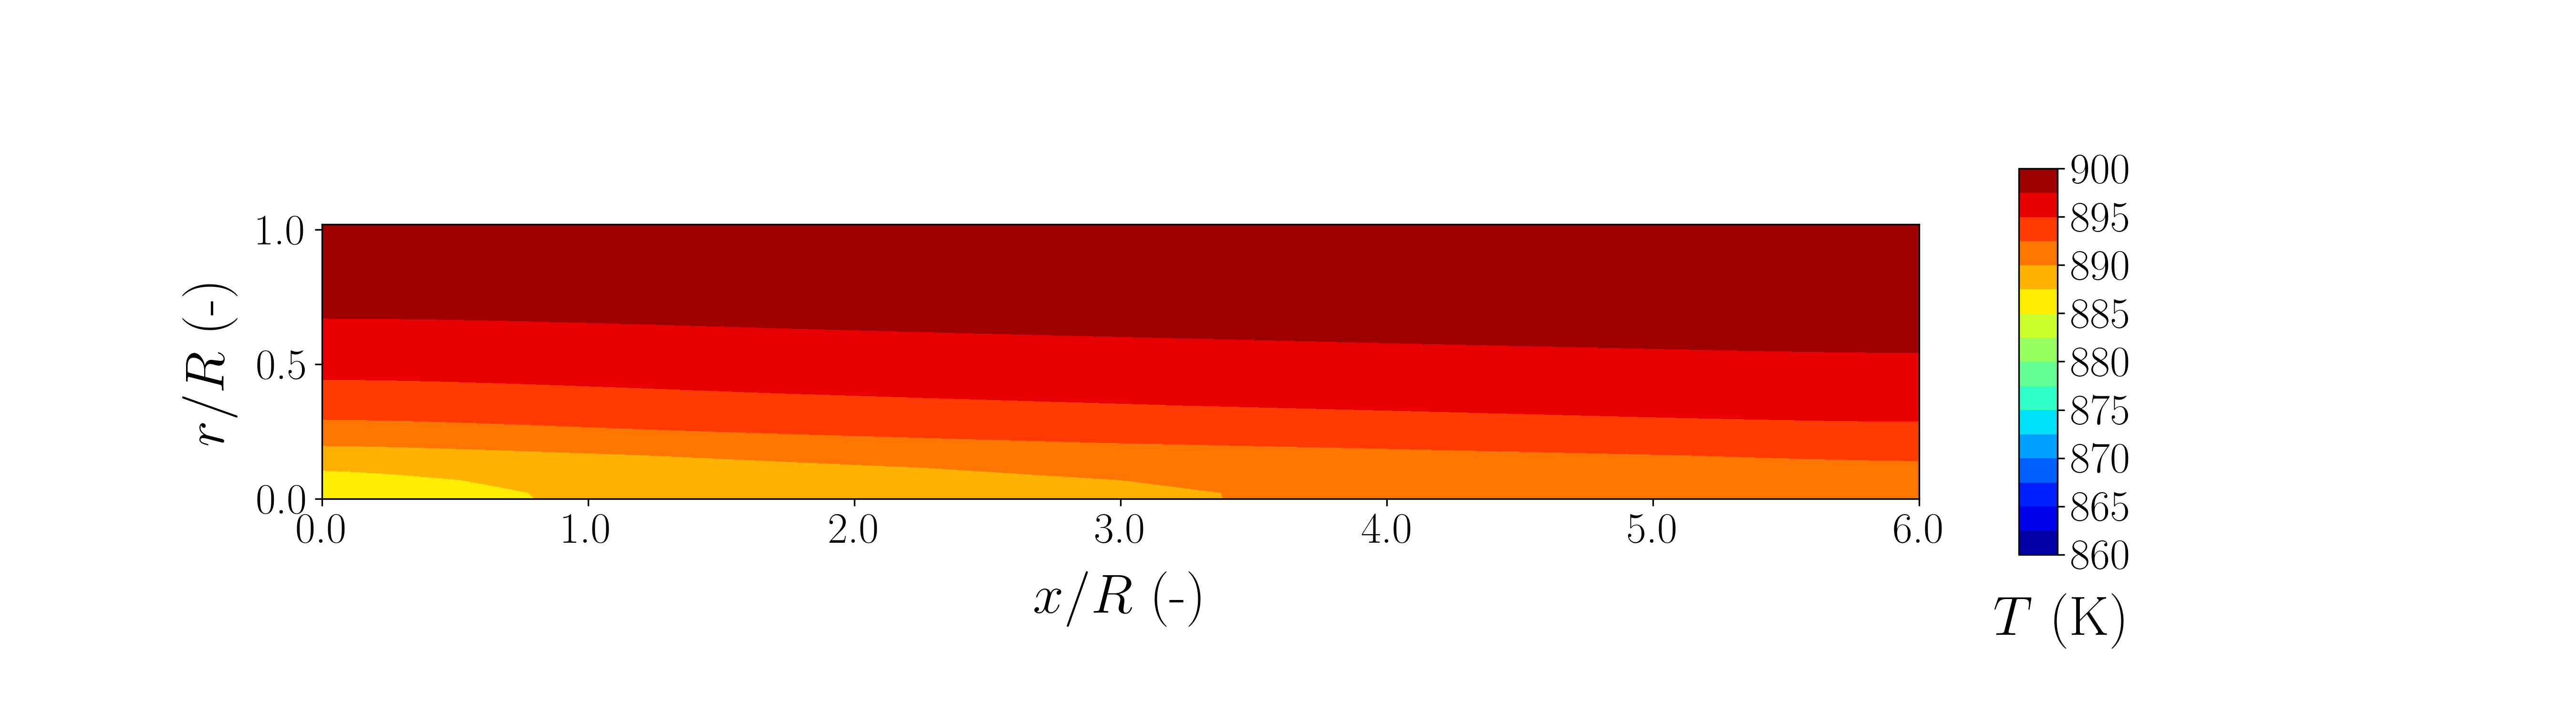
\includegraphics[width=190mm]{results/5/40C_60T/GEN1-TFIELD.png}
\caption{\label{fig:5R4060G1-TField} Strategy I - Temperature field distribution - 1$^{\rm{st}}$ generation ($w_{\rm{CH_4}} = 0.4, w_T = 0.6$, $T_{\rm{in}}$ = 900 K, $u_{\rm{in}}$ = 0.15 m s$^{-1}$, $SC$ = 2.0)}
\end{figure}

\begin{figure}[h!]
\centering
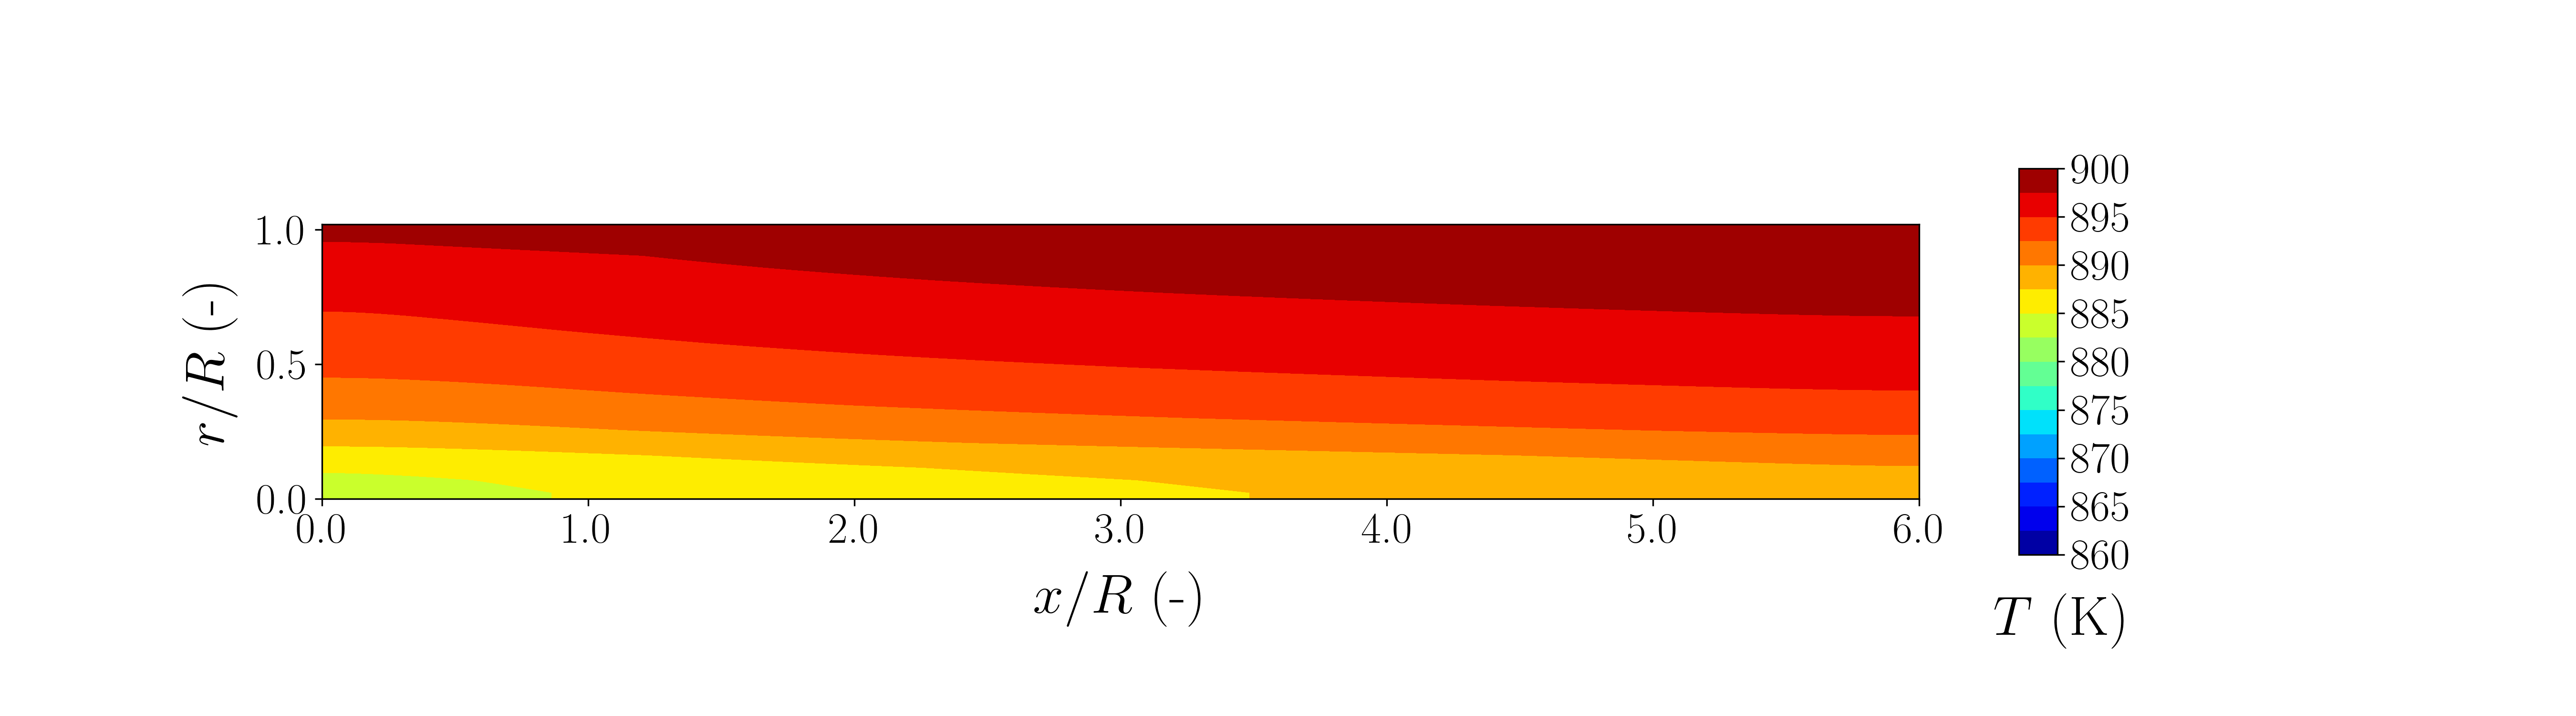
\includegraphics[width=190mm]{results/5/40C_60T/GEN15-TFIELD.png}
\caption{\label{fig:5R4060G15-TField} Strategy I - Temperature field distribution - 15$^{\rm{th}}$ generation ($w_{\rm{CH_4}} = 0.4, w_T = 0.6$, $T_{\rm{in}}$ = 900 K, $u_{\rm{in}}$ = 0.15 m s$^{-1}$, $SC$ = 2.0)}
\end{figure}

\begin{figure}[h!]
\centering
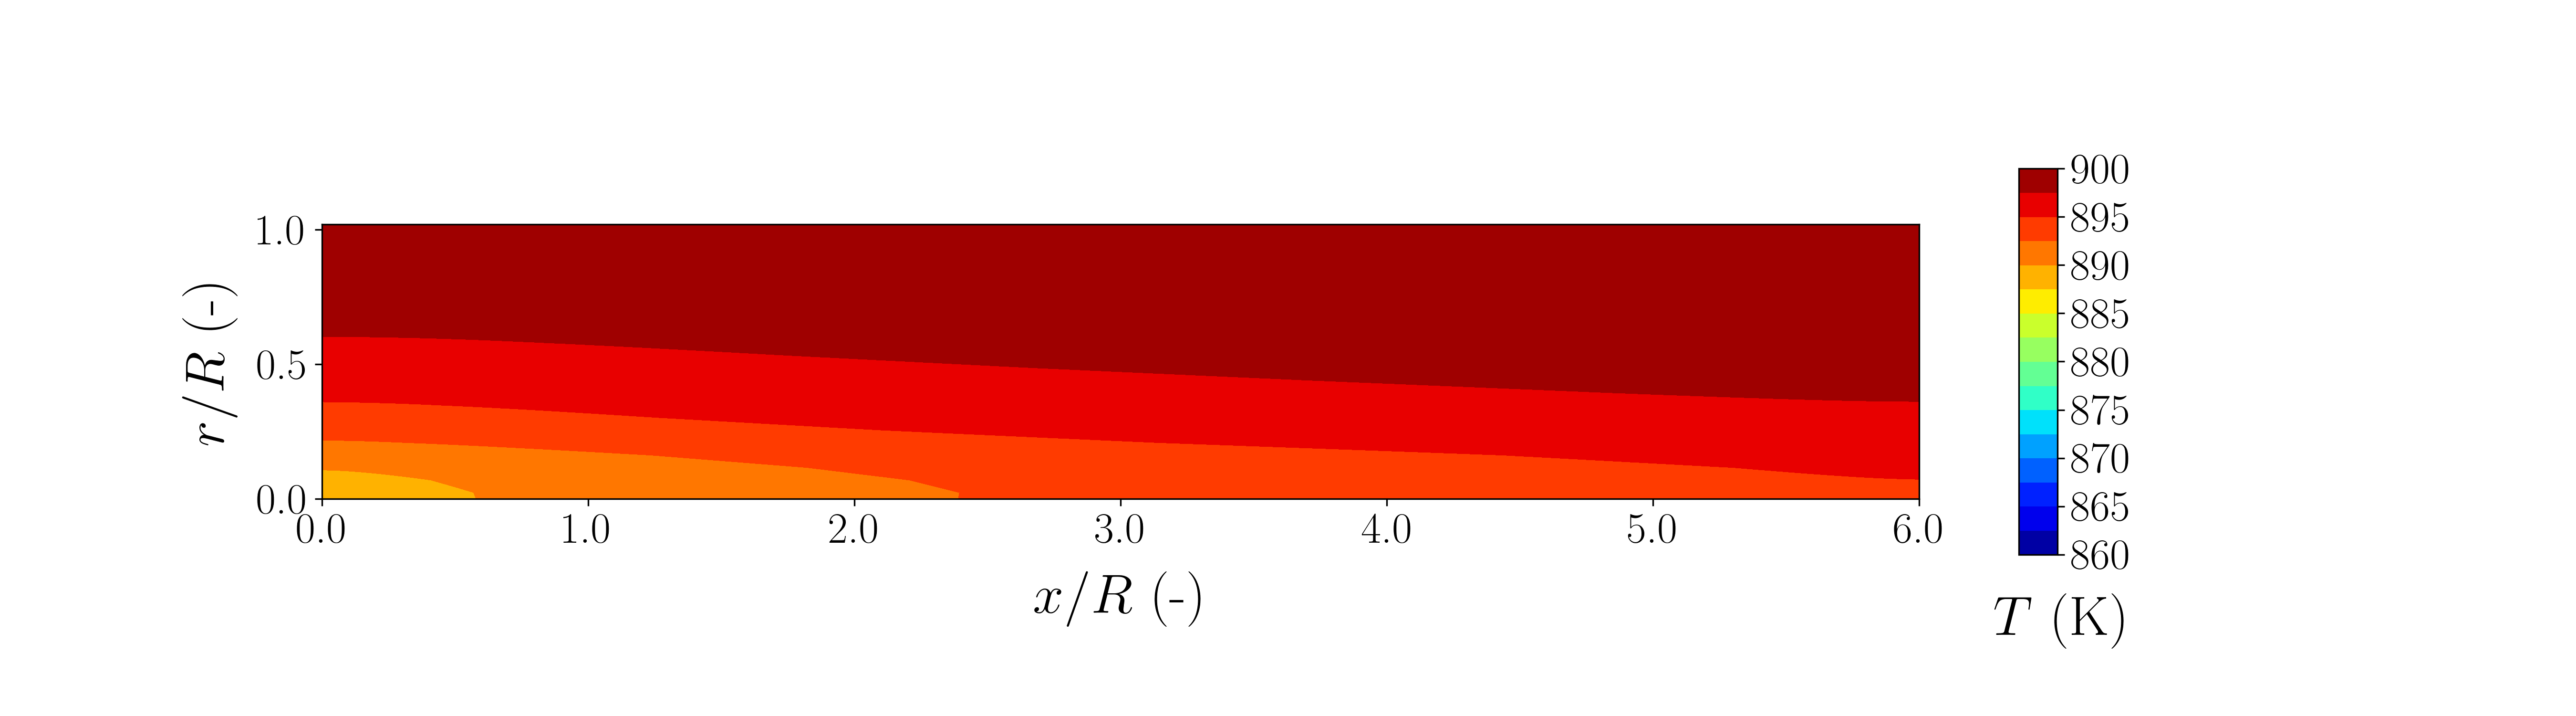
\includegraphics[width=190mm]{results/5/40C_60T/GEN30-TFIELD.png}
\caption{\label{fig:5R4060G30-TField} Strategy I - Temperature field distribution - 30$^{\rm{th}}$ generation ($w_{\rm{CH_4}} = 0.4, w_T = 0.6$, $T_{\rm{in}}$ = 900 K, $u_{\rm{in}}$ = 0.15 m s$^{-1}$, $SC$ = 2.0)}
\end{figure}


\begin{figure}[h!]
\centering
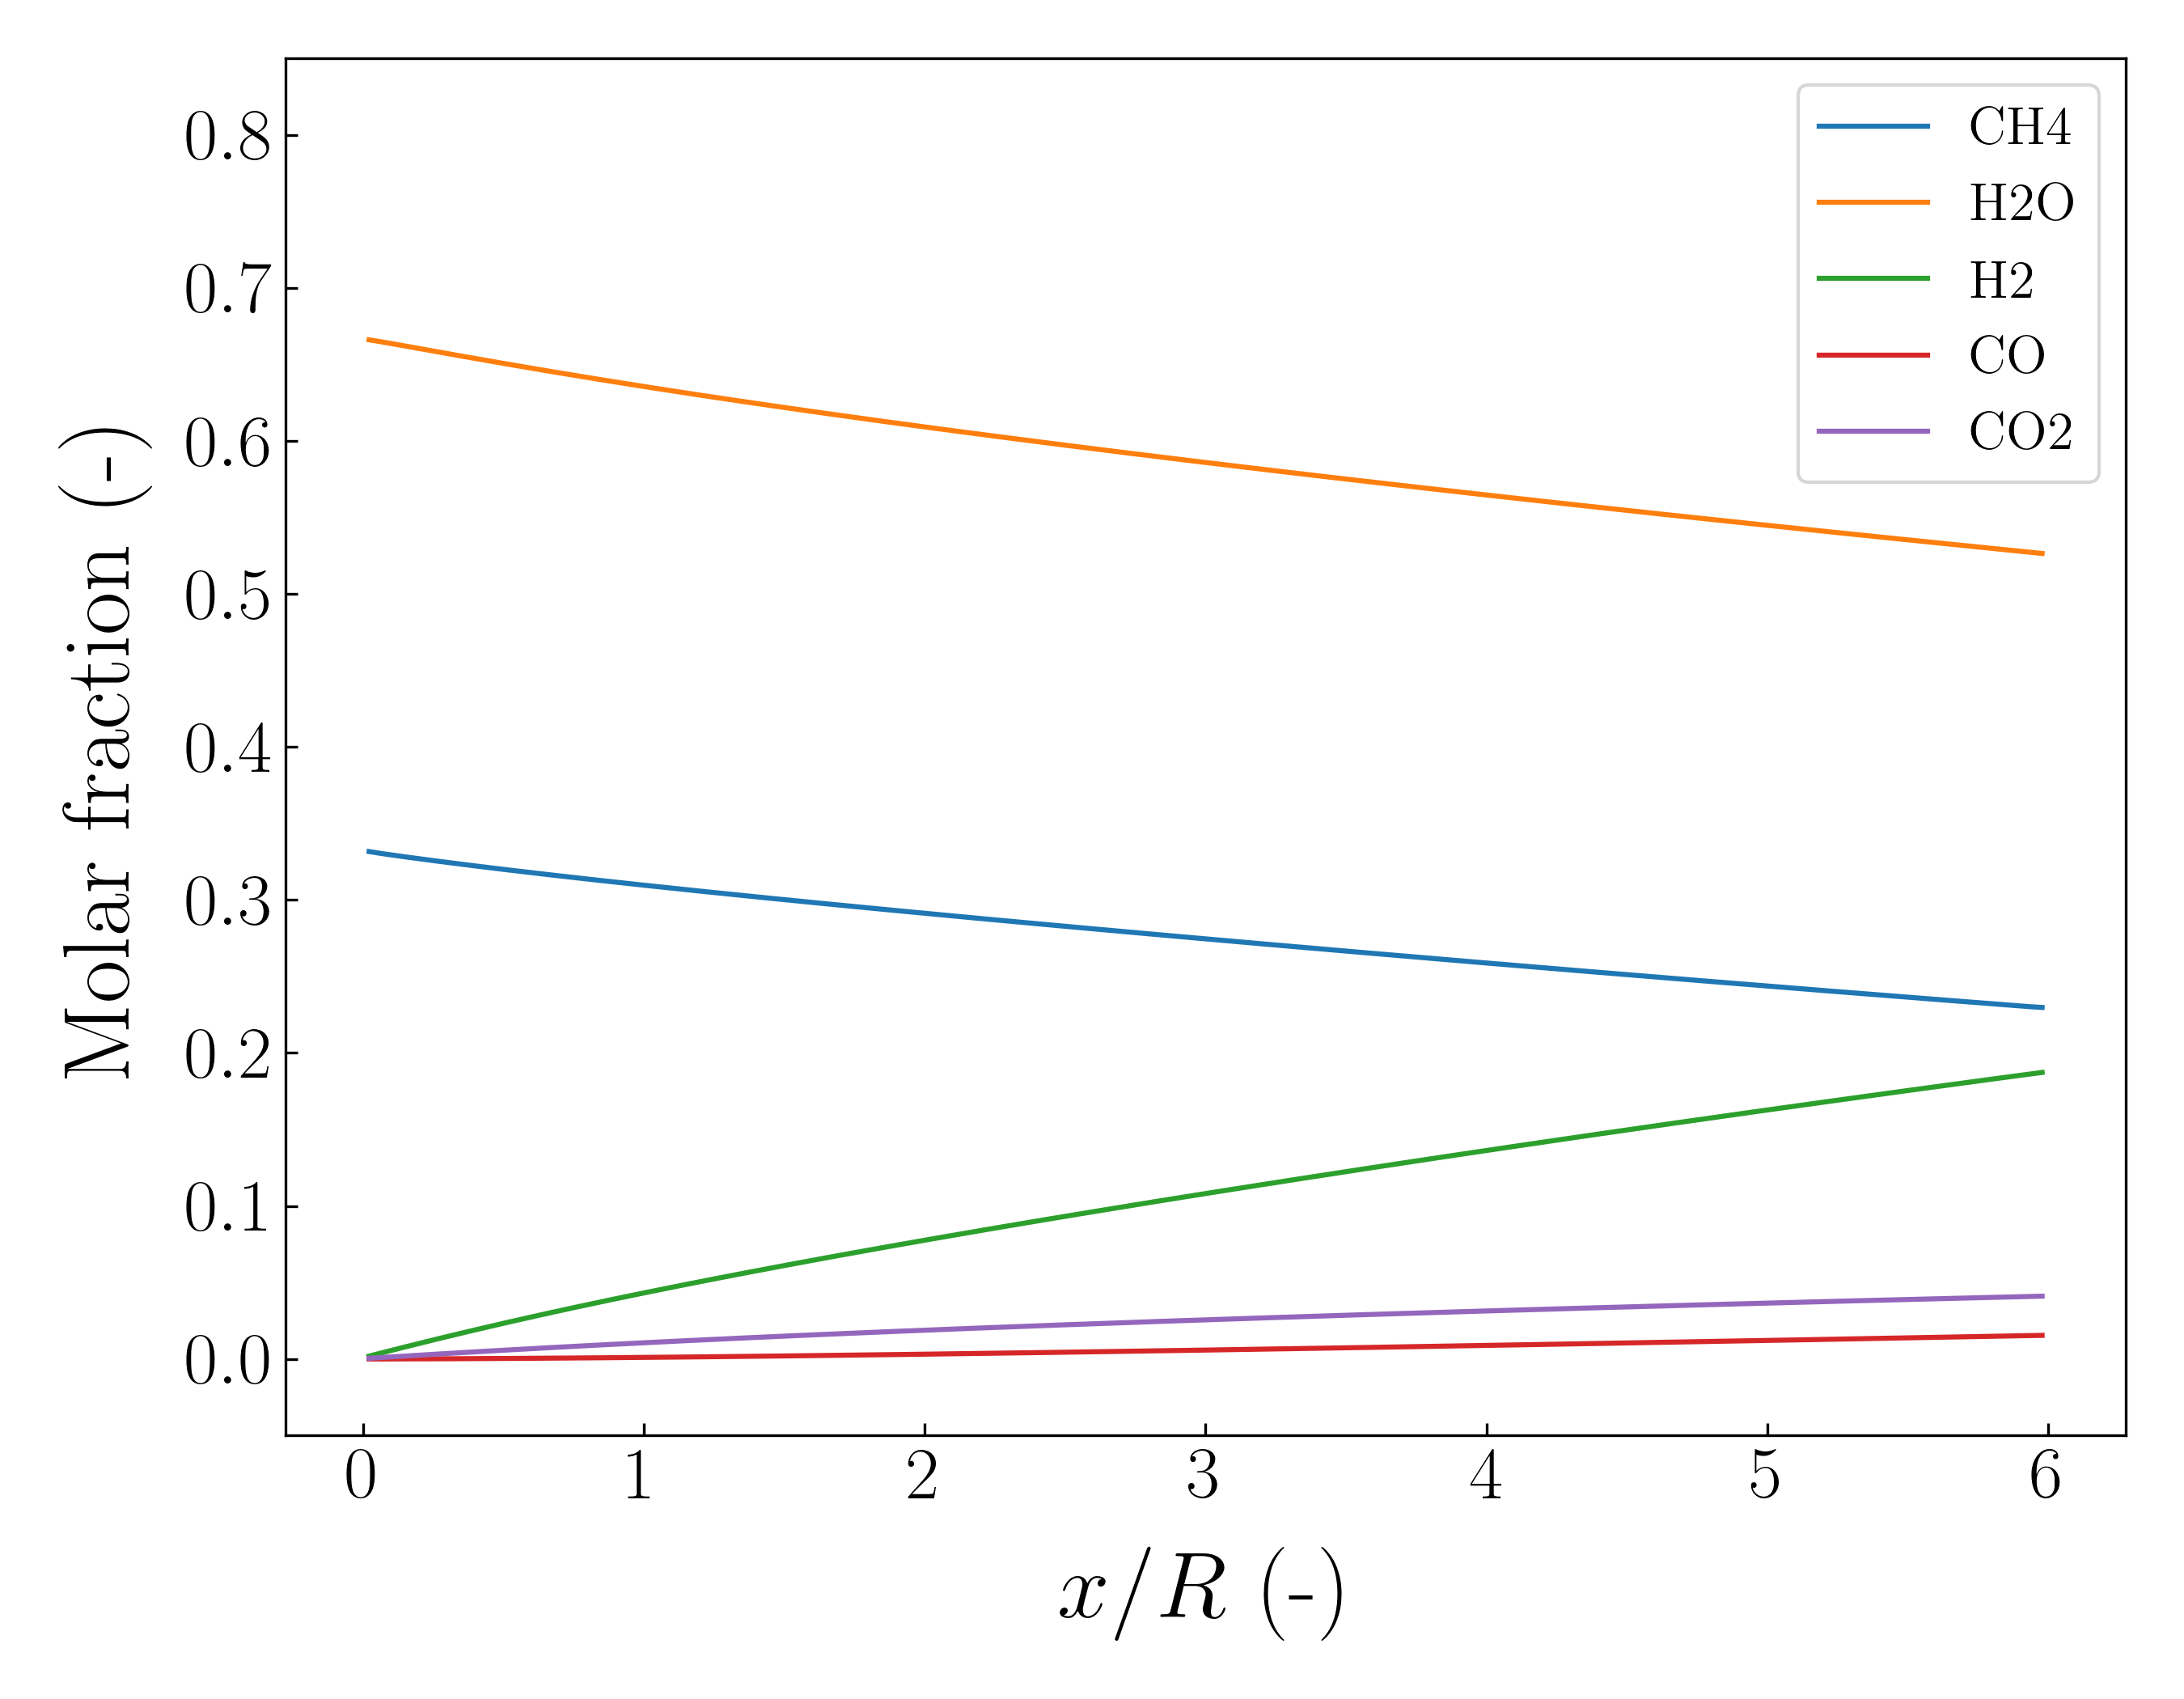
\includegraphics[width=80mm]{results/5/40C_60T/GEN1-AVG.png}
\caption{\label{fig:5R4060G1-avg} Strategy I - Radius-averaged molar fractions - 1$^{\rm{st}}$ generation ($w_{\rm{CH_4}} = 0.4, w_T = 0.6$, $T_{\rm{in}}$ = 900 K, $u_{\rm{in}}$ = 0.15 m s$^{-1}$, $SC$ = 2.0)}
\end{figure}

\begin{figure}[h!]
\centering
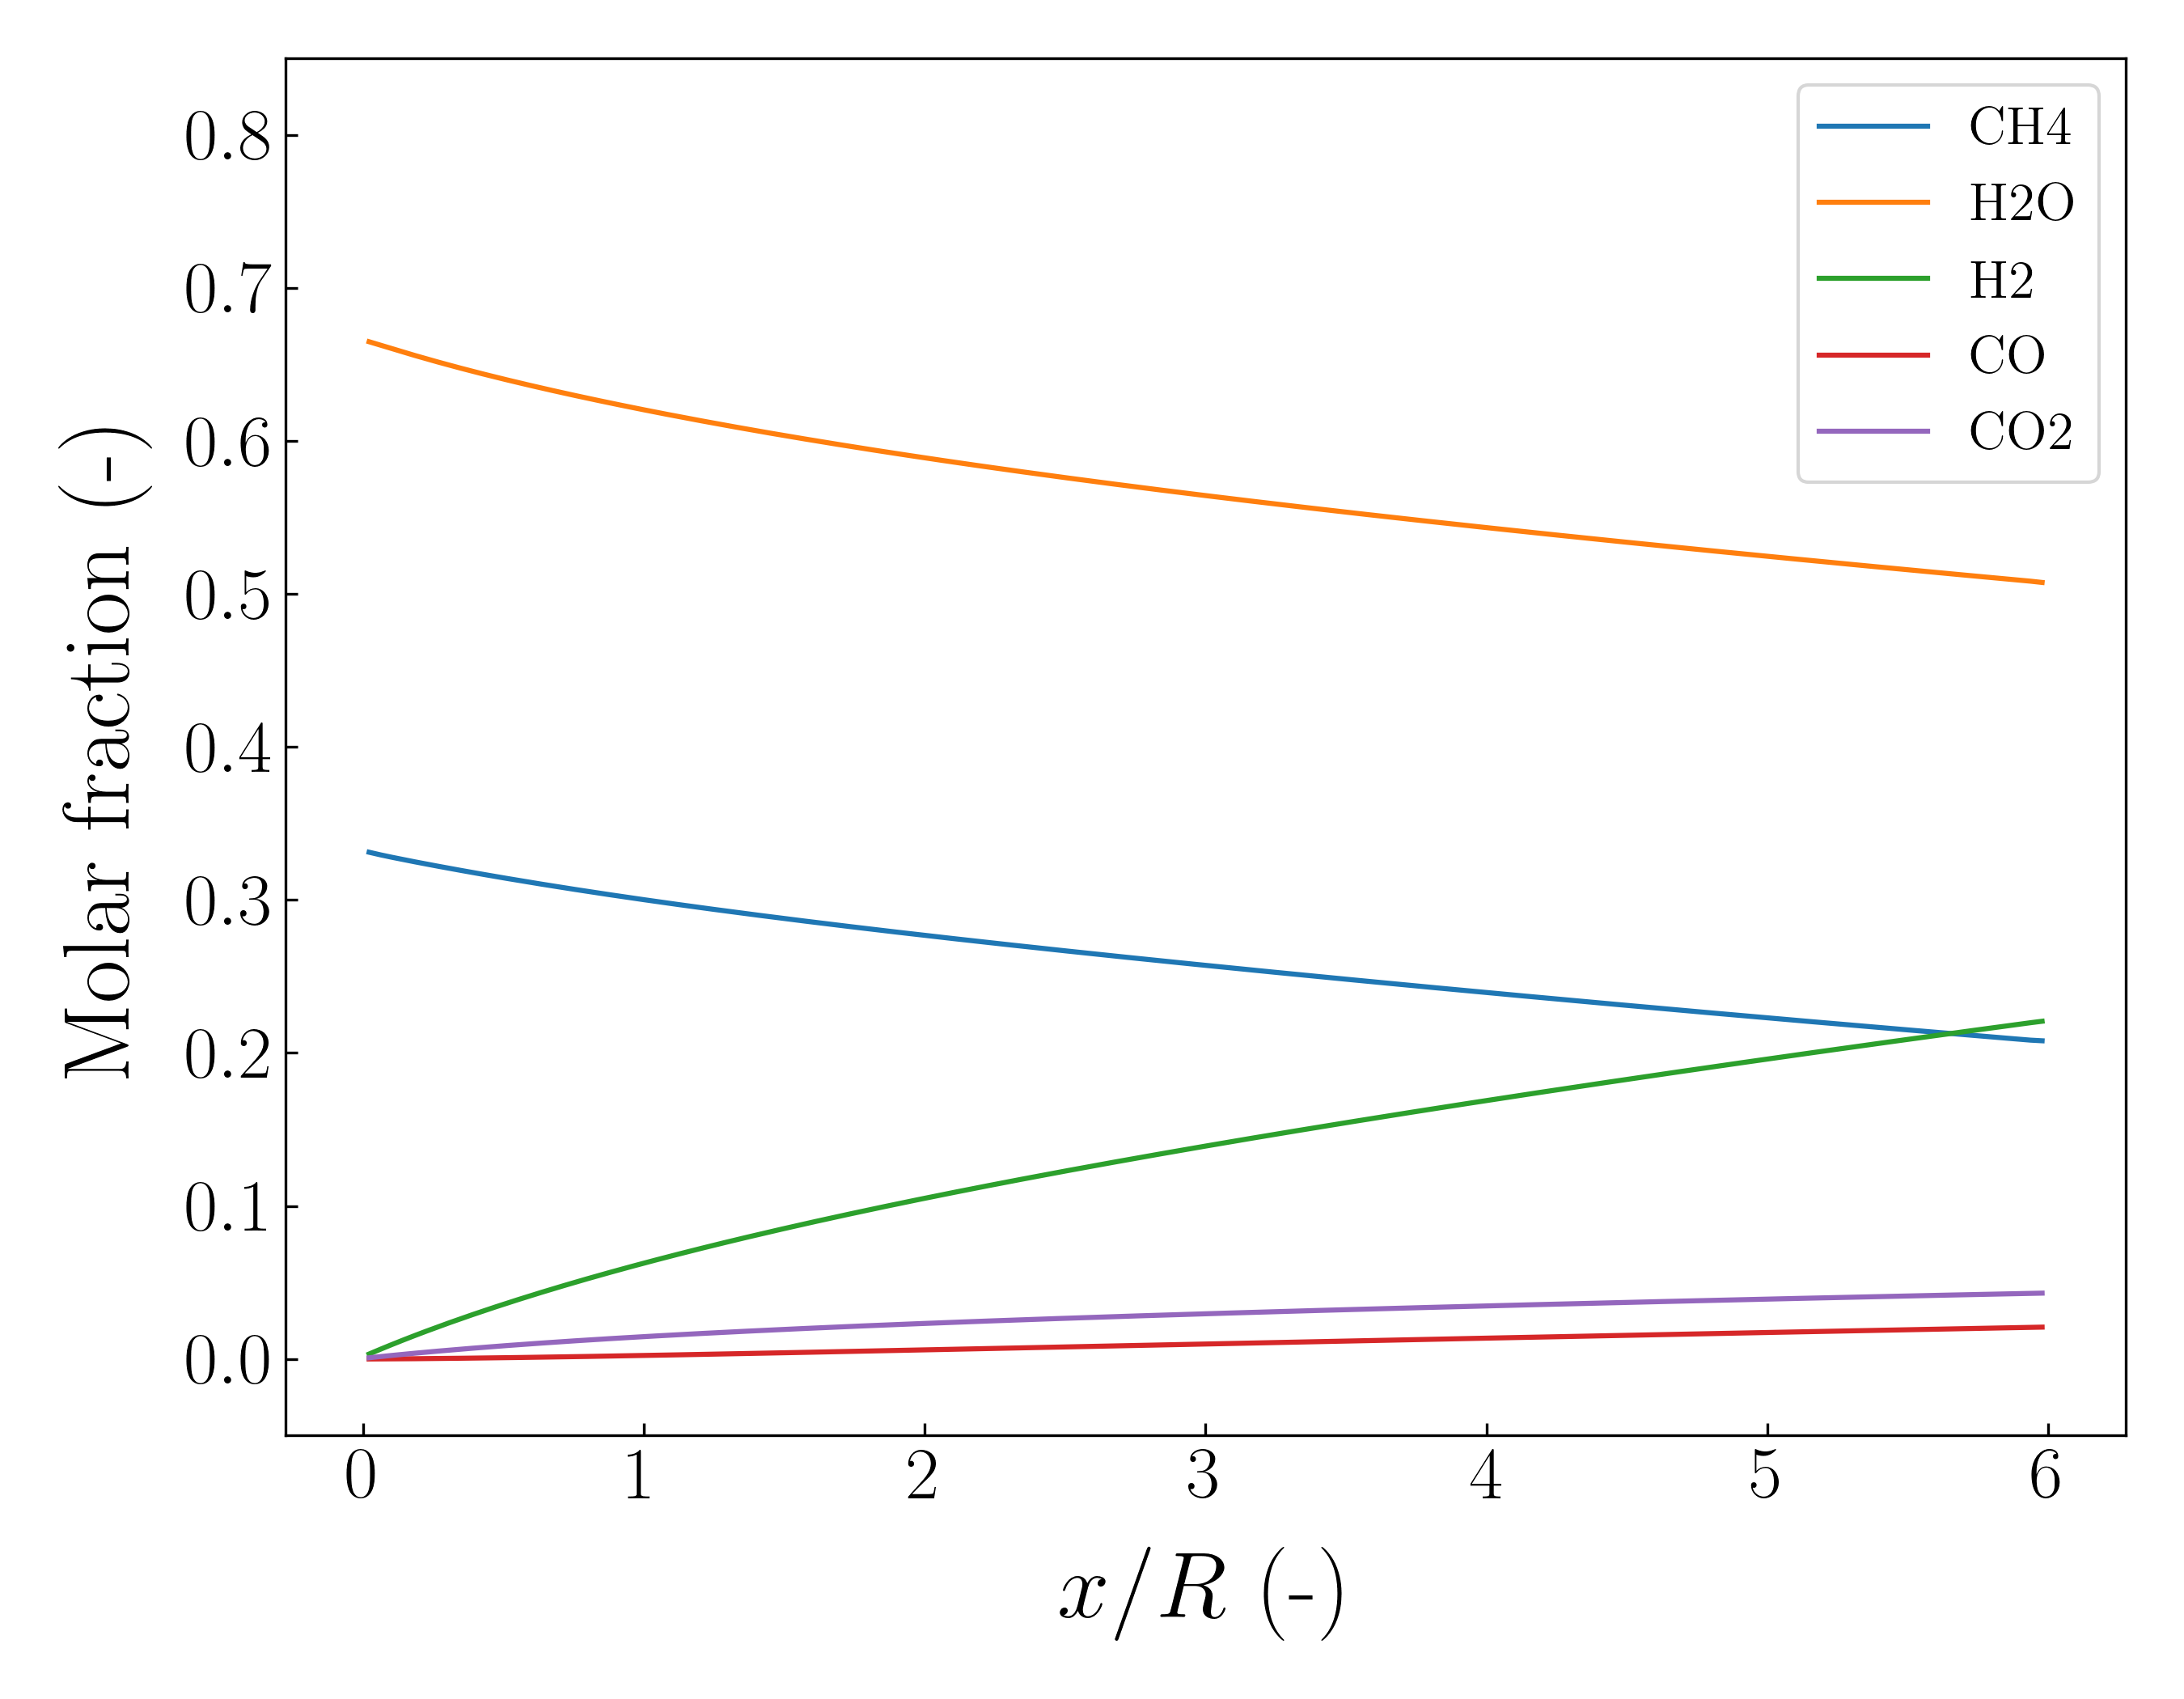
\includegraphics[width=80mm]{results/5/40C_60T/GEN15-AVG.png}
\caption{\label{fig:5R4060G15-avg} Strategy I - Radius-averaged molar fractions - 15$^{\rm{th}}$ generation ($w_{\rm{CH_4}} = 0.4, w_T = 0.6$, $T_{\rm{in}}$ = 900 K, $u_{\rm{in}}$ = 0.15 m s$^{-1}$, $SC$ = 2.0)}
\end{figure}

\begin{figure}[h!]
\centering
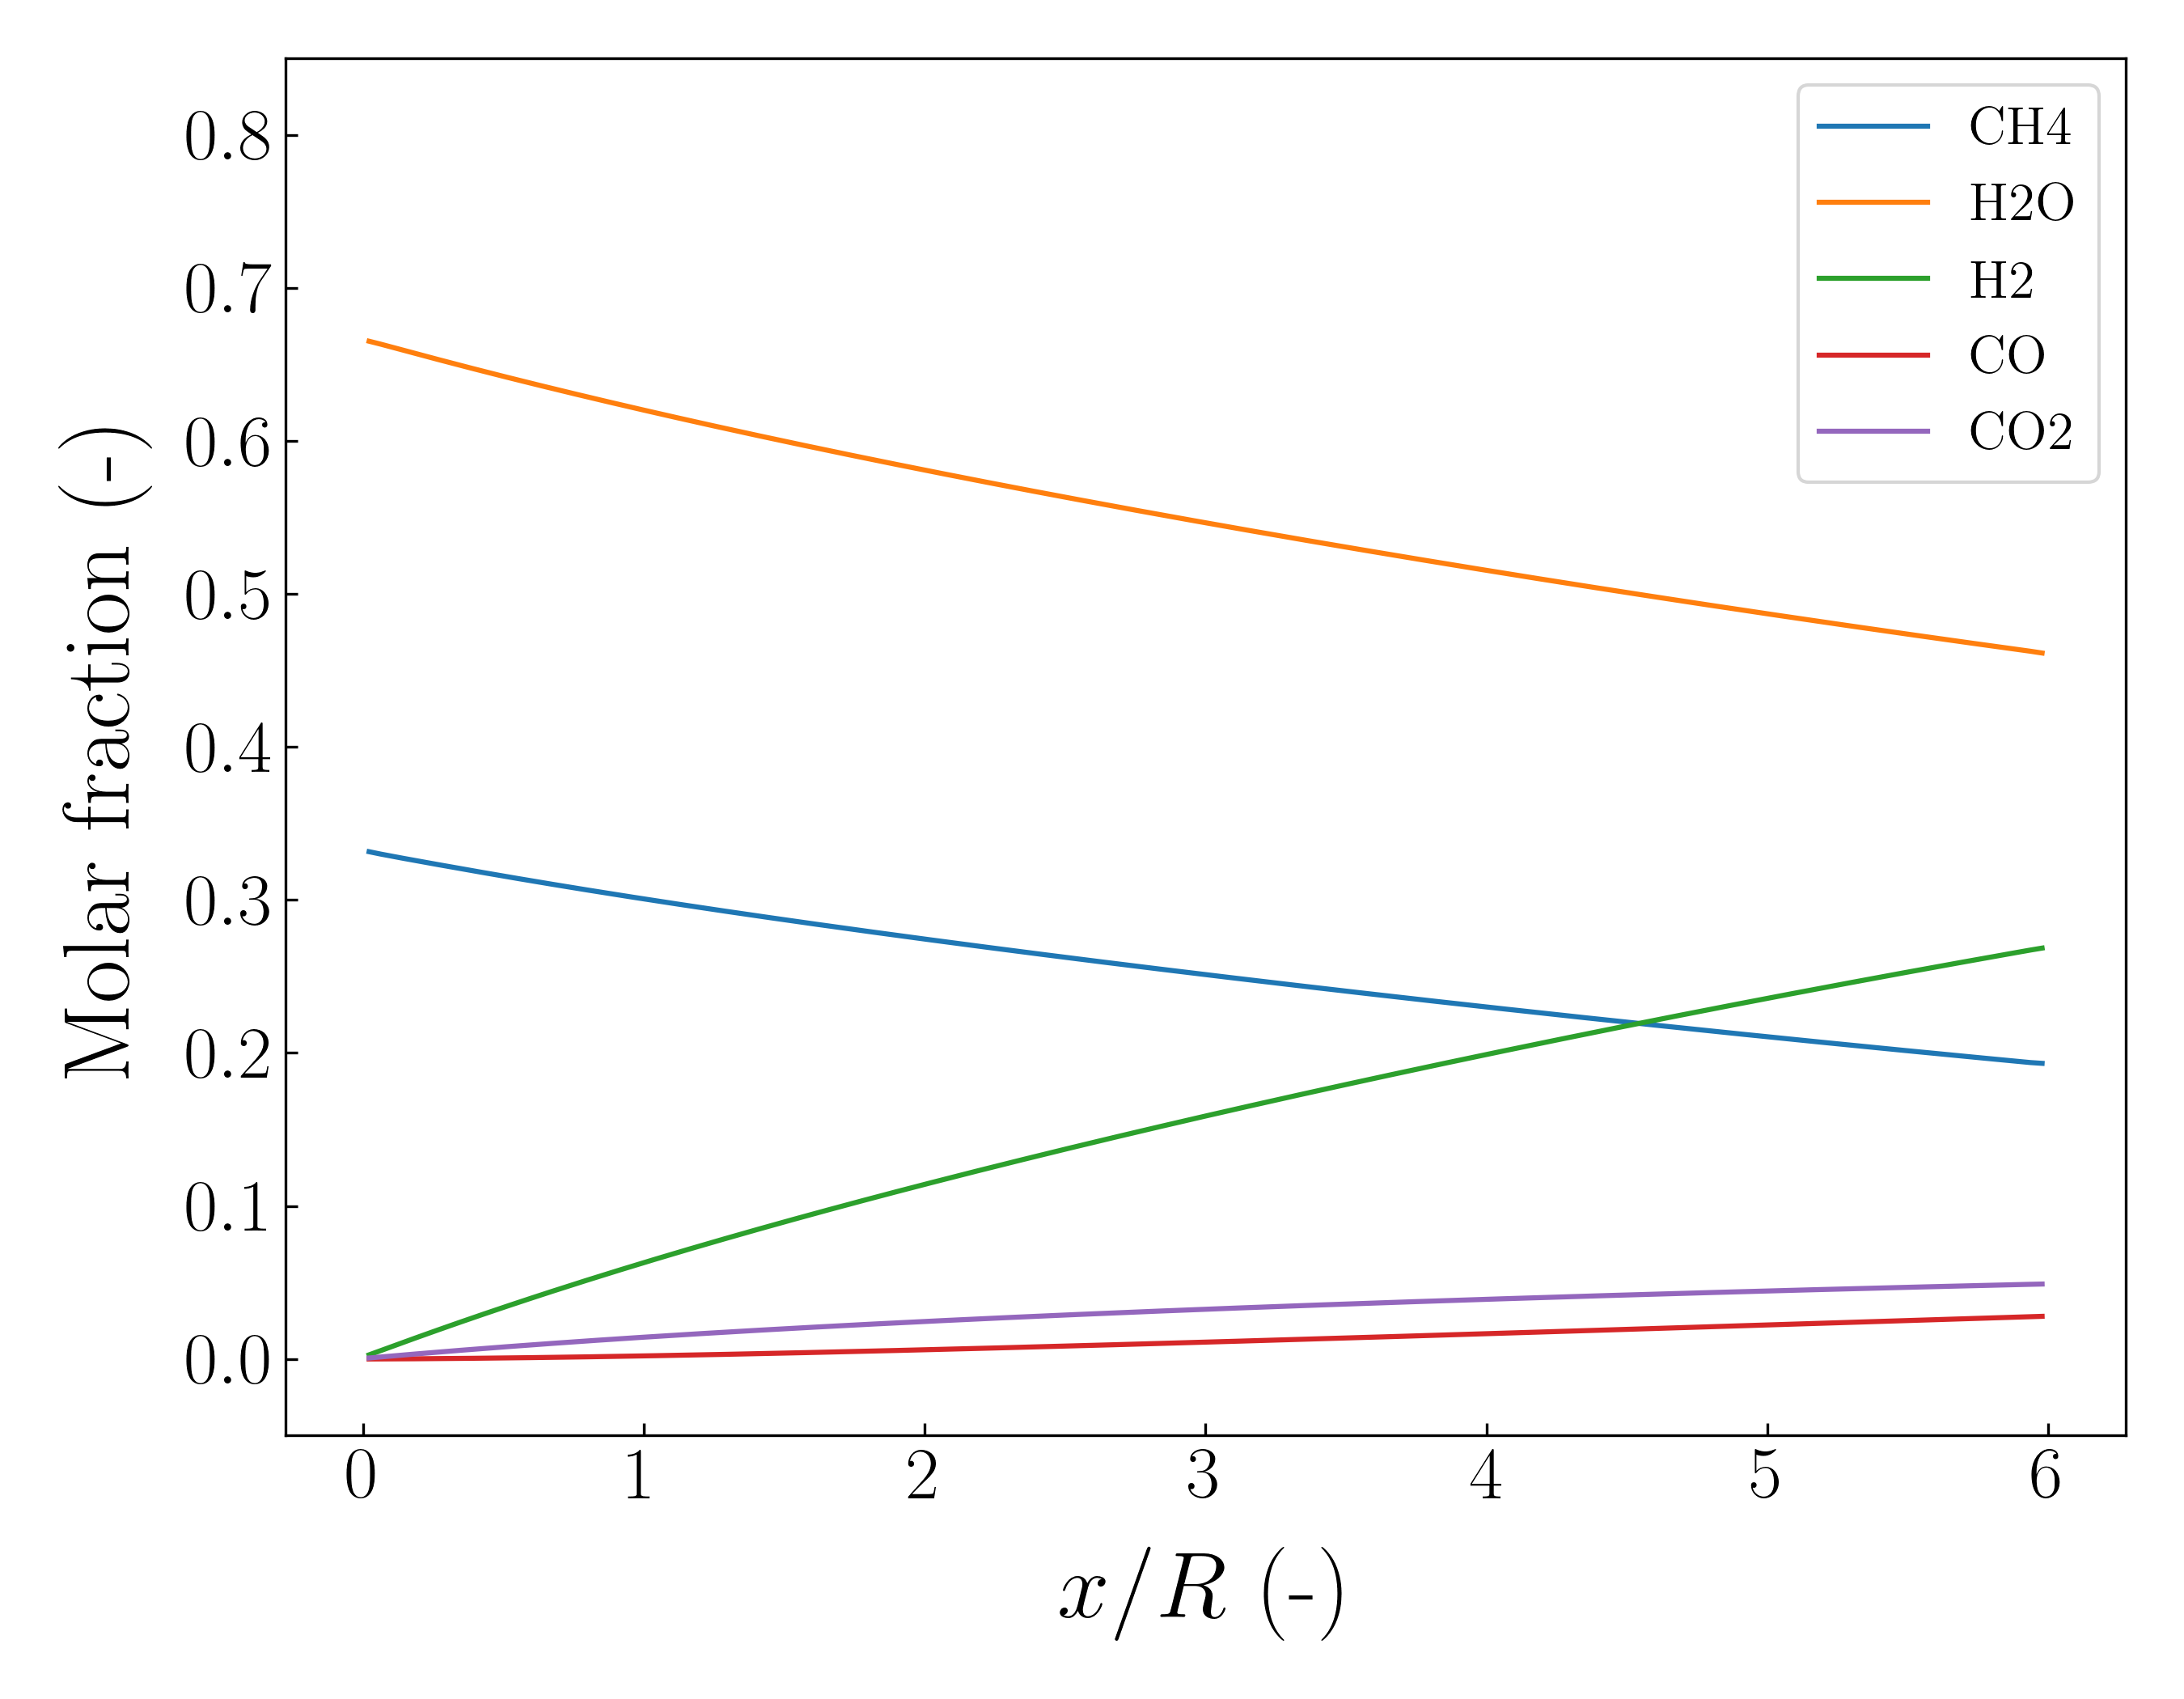
\includegraphics[width=80mm]{results/5/40C_60T/GEN30-AVG.png}
\caption{\label{fig:5R4060G30-avg} Strategy I - Radius-averaged molar fractions -  30$^{\rm{th}}$ generation ($w_{\rm{CH_4}} = 0.4, w_T = 0.6$, $T_{\rm{in}}$ = 900 K, $u_{\rm{in}}$ = 0.15 m s$^{-1}$, $SC$ = 2.0)}
\end{figure}

\begin{figure}[h!]
\centering
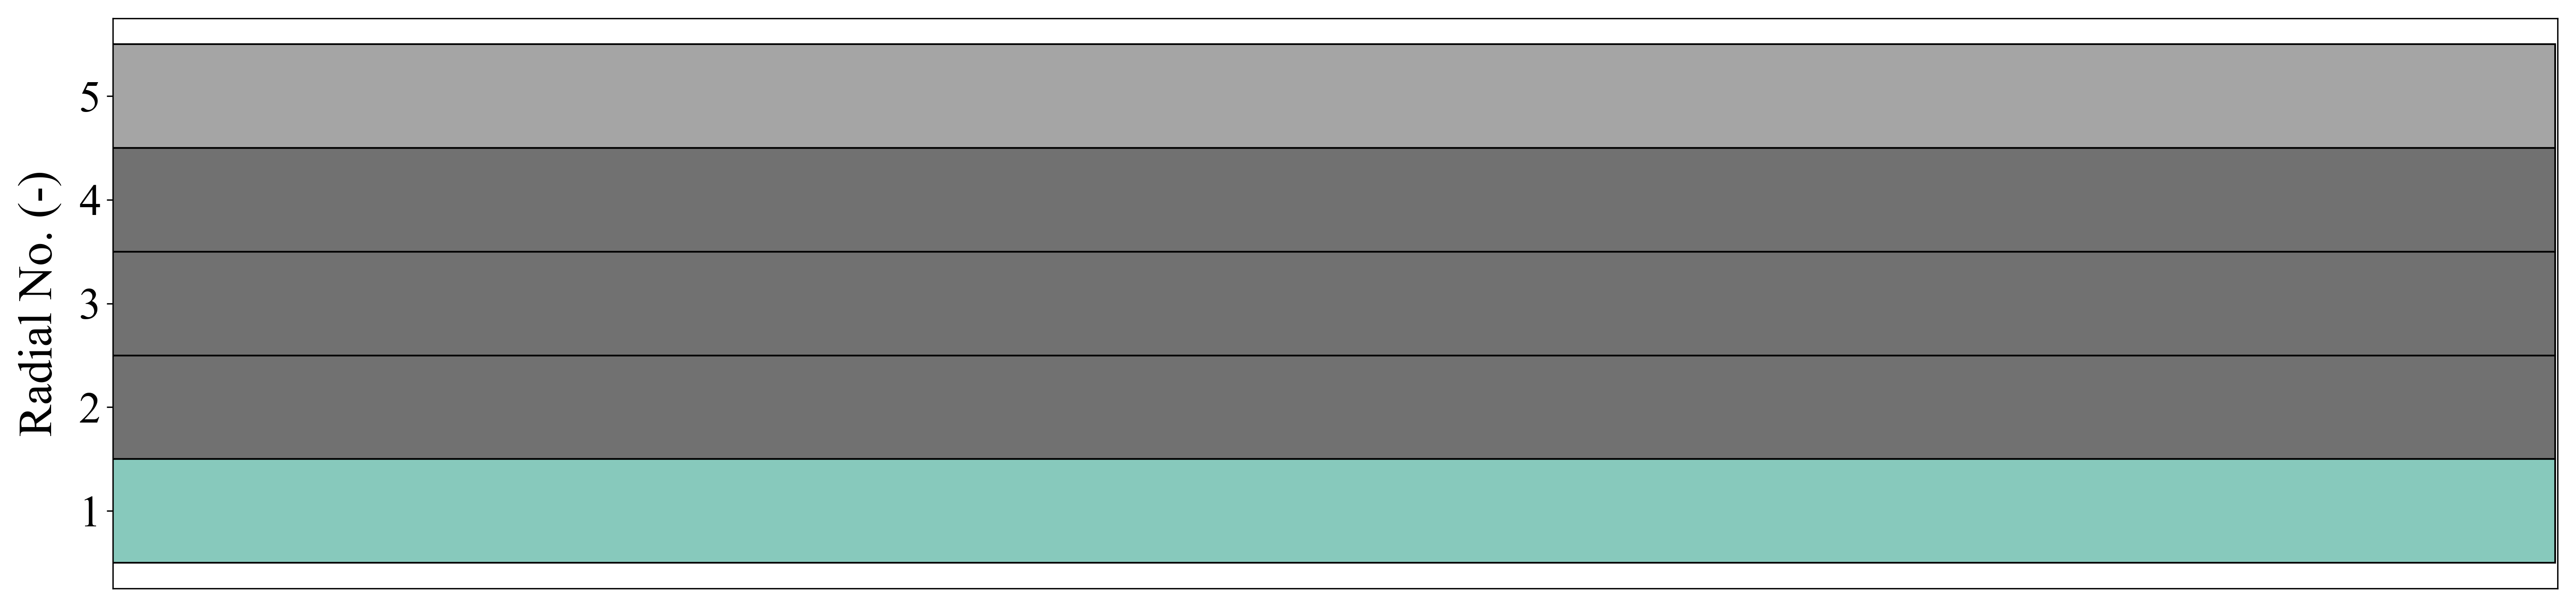
\includegraphics[width=120mm]{results/segments/5seg/40C60T/seg.png}
\caption{\label{fig:30L6040G1-TField} Strategy I - Segments distribution for 30$^{\rm{th}}$ generation ($w_{\rm{CH_4}} = 0.4, w_T = 0.6$, $T_{\rm{in}}$ = 900 K, $u_{\rm{in}}$ = 0.15 m s$^{-1}$, $SC$ = 2.0)}
\end{figure}

%\begin{figure}[h!]
%\centering
%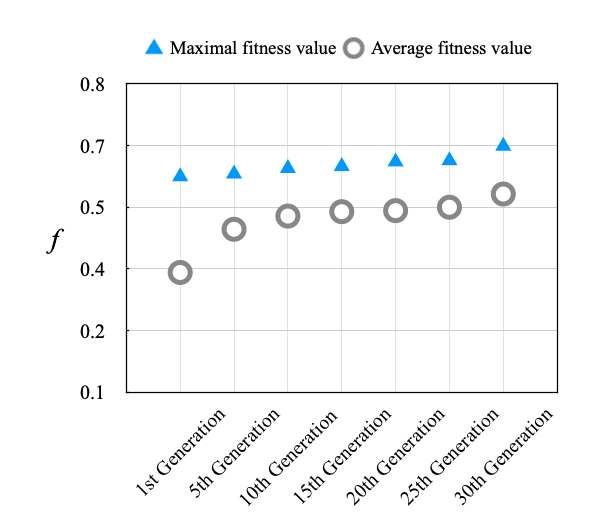
\includegraphics[width=100mm]{results/5/40C_60T.png}
%\caption{\label{fig:5R4060G-fitness} Strategy I - Fitness analysis throughout successive populations ($w_{\rm{CH_4}} = 0.4, w_T = 0.6$, $T_{\rm{in}}$ = 900 K, $u_{\rm{in}}$ = 0.15 m s$^{-1}$, $SC$ = 2.0)}
%\end{figure}


\clearpage





\paragraph{Thermal fitness 50 \%, methane conversion 50 \%} \hspace{0pt} \\
\noindent 


\begin{figure}[h!]
\centering
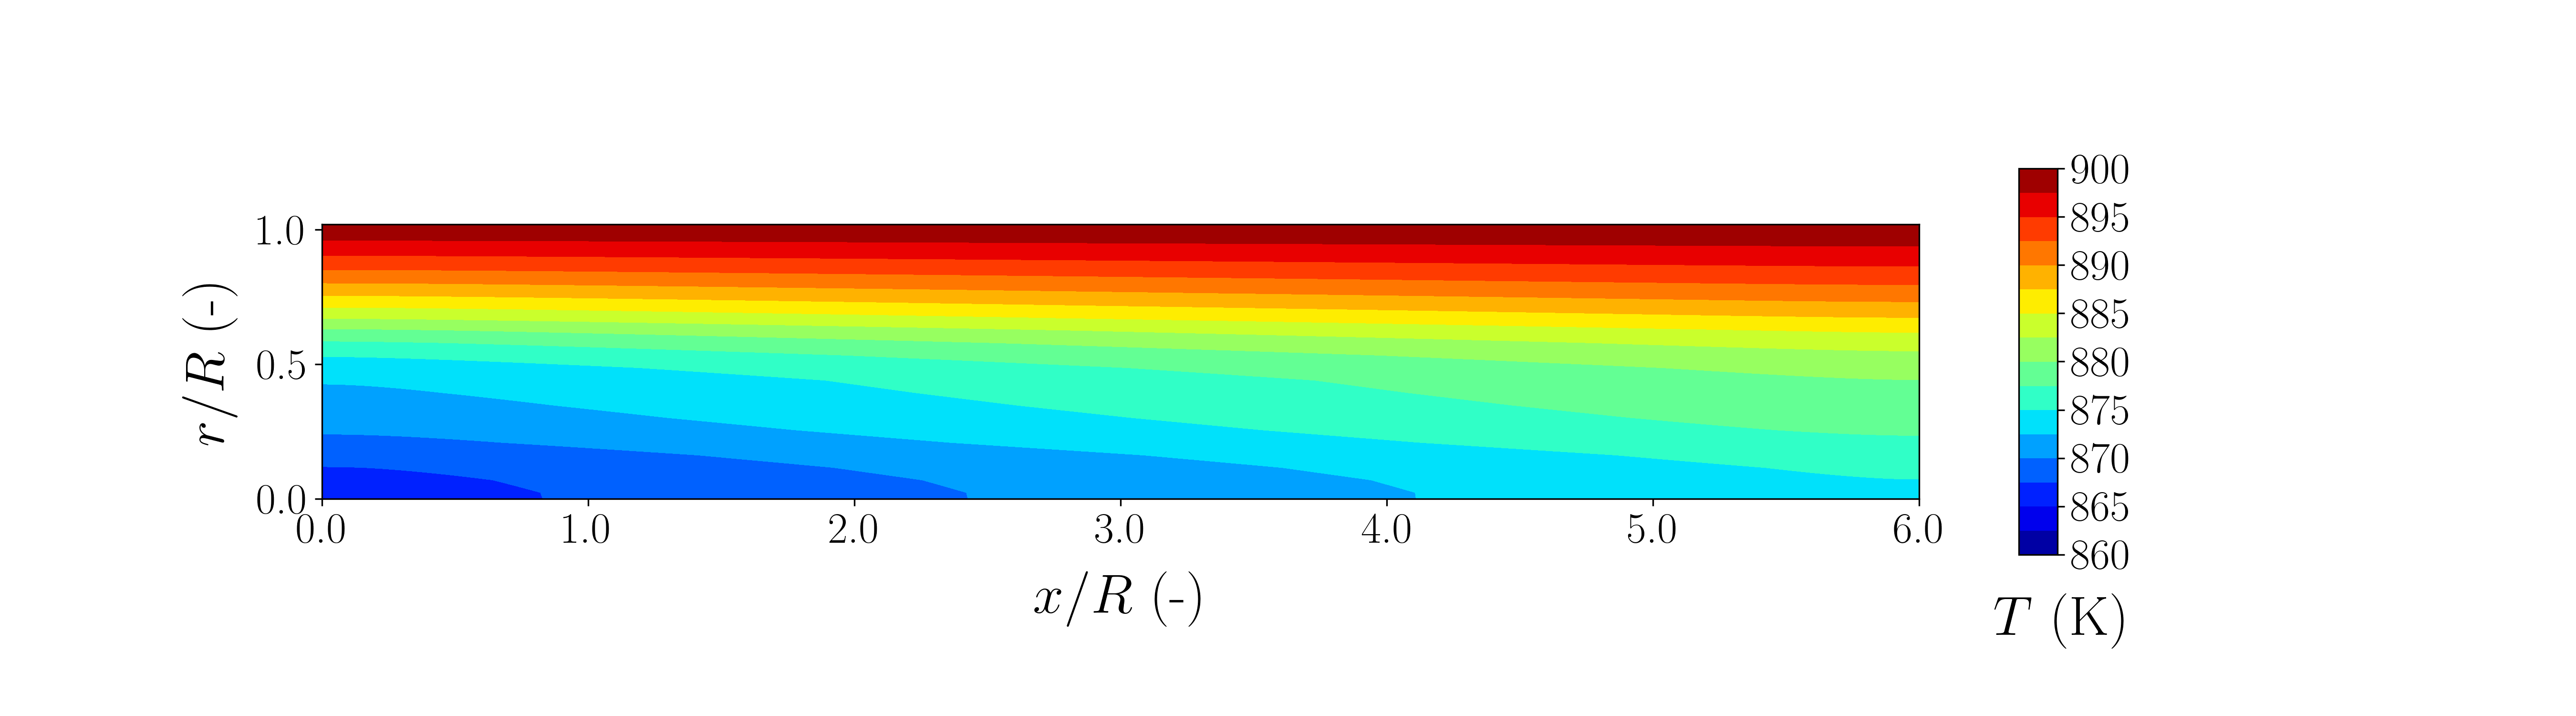
\includegraphics[width=190mm]{results/5/50C_50T/GEN1-TFIELD.png}
\caption{\label{fig:5R5050G1-TField} Strategy I - Temperature field distribution - 1$^{\rm{st}}$ generation ($w_{\rm{CH_4}} = 0.5, w_T = 0.5$, $T_{\rm{in}}$ = 900 K, $u_{\rm{in}}$ = 0.15 m s$^{-1}$, $SC$ = 2.0)}
\end{figure}

\begin{figure}[h!]
\centering
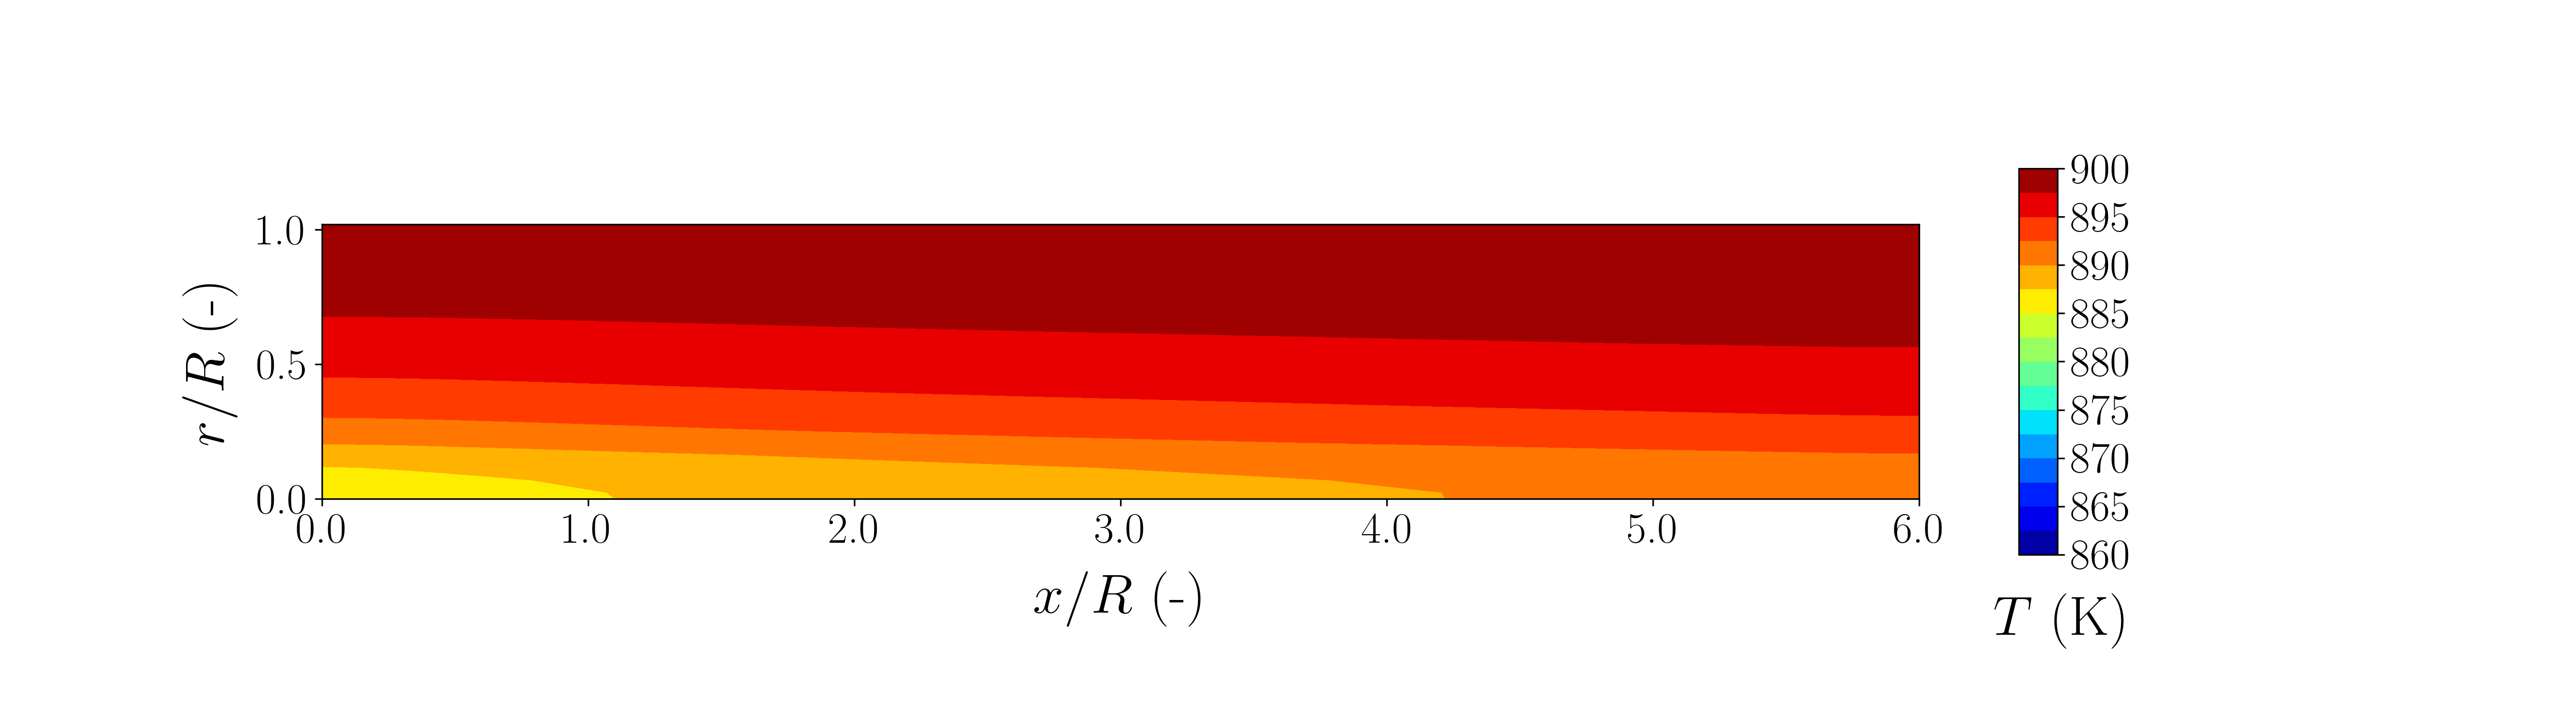
\includegraphics[width=190mm]{results/5/50C_50T/GEN15-TFIELD.png}
\caption{\label{fig:5R5050G15-TField} Strategy I - Temperature field distribution - 15$^{\rm{th}}$ generation ($w_{\rm{CH_4}} = 0.5, w_T = 0.5$, $T_{\rm{in}}$ = 900 K, $u_{\rm{in}}$ = 0.15 m s$^{-1}$, $SC$ = 2.0)}
\end{figure}

\begin{figure}[h!]
\centering
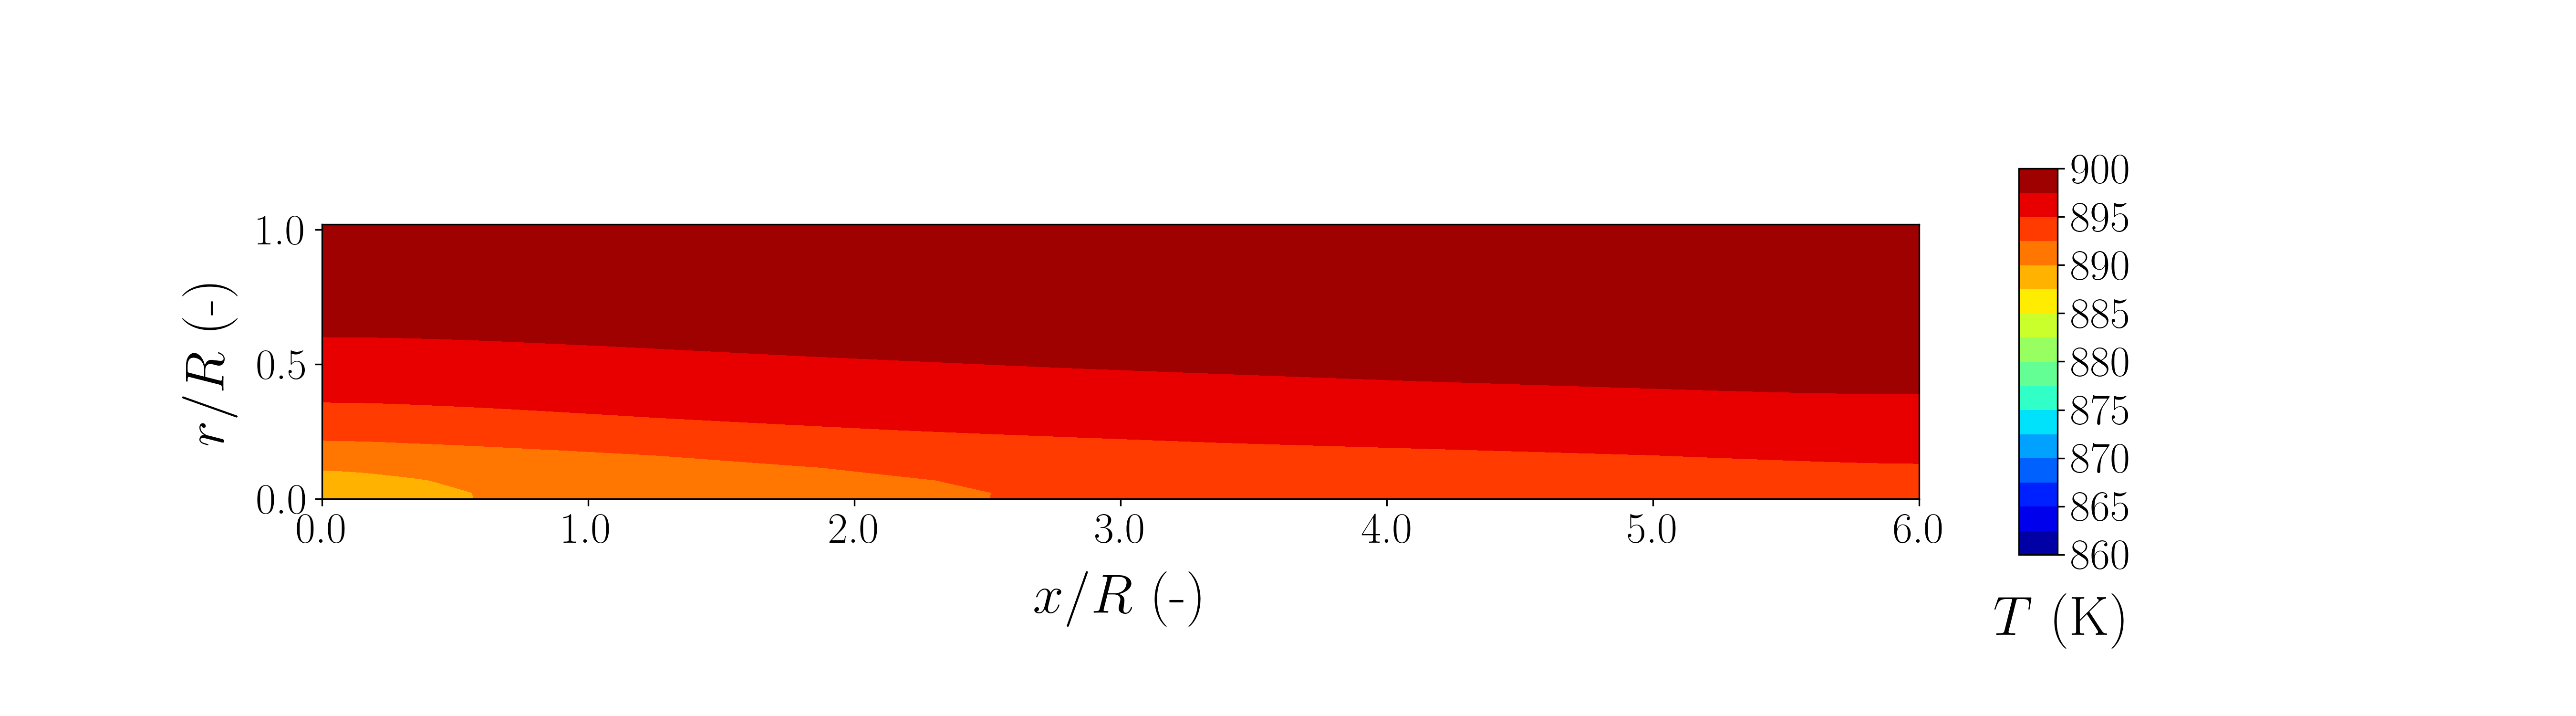
\includegraphics[width=190mm]{results/5/50C_50T/GEN30-TFIELD.png}
\caption{\label{fig:5R5050G30-TField} Strategy I - Temperature field distribution - 30$^{\rm{th}}$ generation ($w_{\rm{CH_4}} = 0.5, w_T = 0.5$, $T_{\rm{in}}$ = 900 K, $u_{\rm{in}}$ = 0.15 m s$^{-1}$, $SC$ = 2.0)}
\end{figure}


\begin{figure}[h!]
\centering
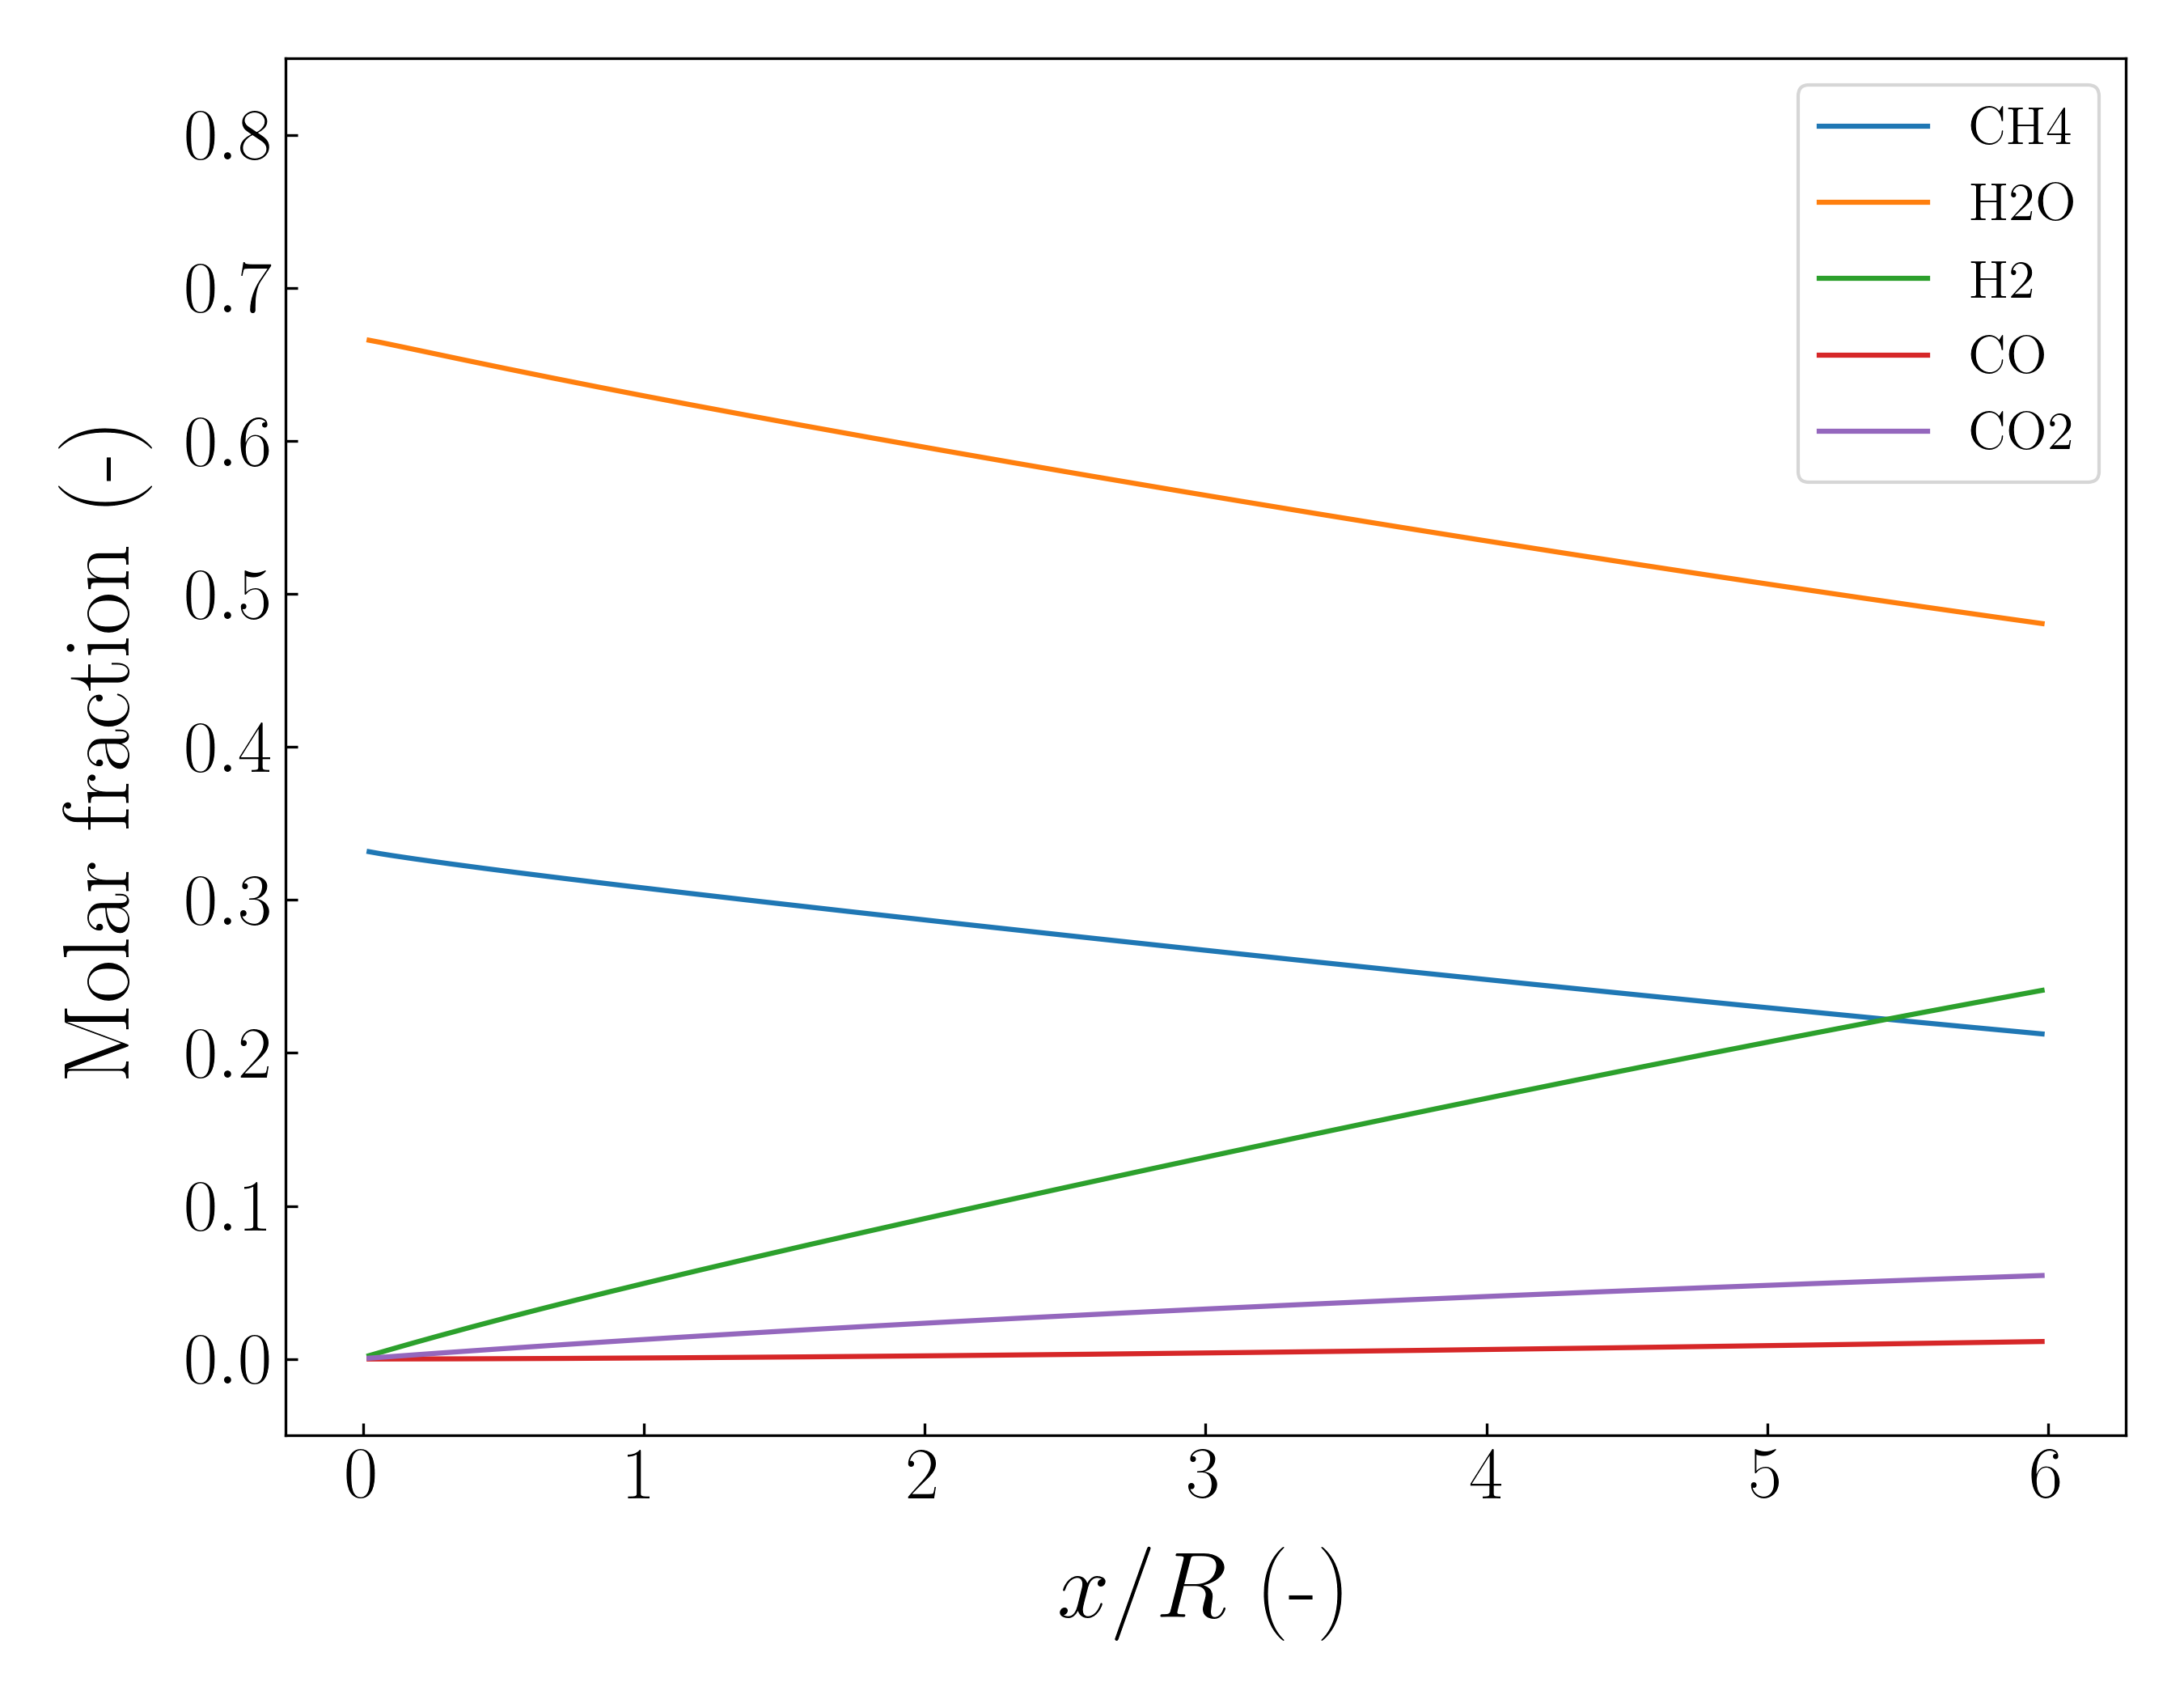
\includegraphics[width=80mm]{results/5/50C_50T/GEN1-AVG.png}
\caption{\label{fig:5R5050G1-avg} Strategy I - Radius-averaged molar fractions - 1$^{\rm{st}}$ generation ($w_{\rm{CH_4}} = 0.5, w_T = 0.5$, $T_{\rm{in}}$ = 900 K, $u_{\rm{in}}$ = 0.15 m s$^{-1}$, $SC$ = 2.0)}
\end{figure}

\begin{figure}[h!]
\centering
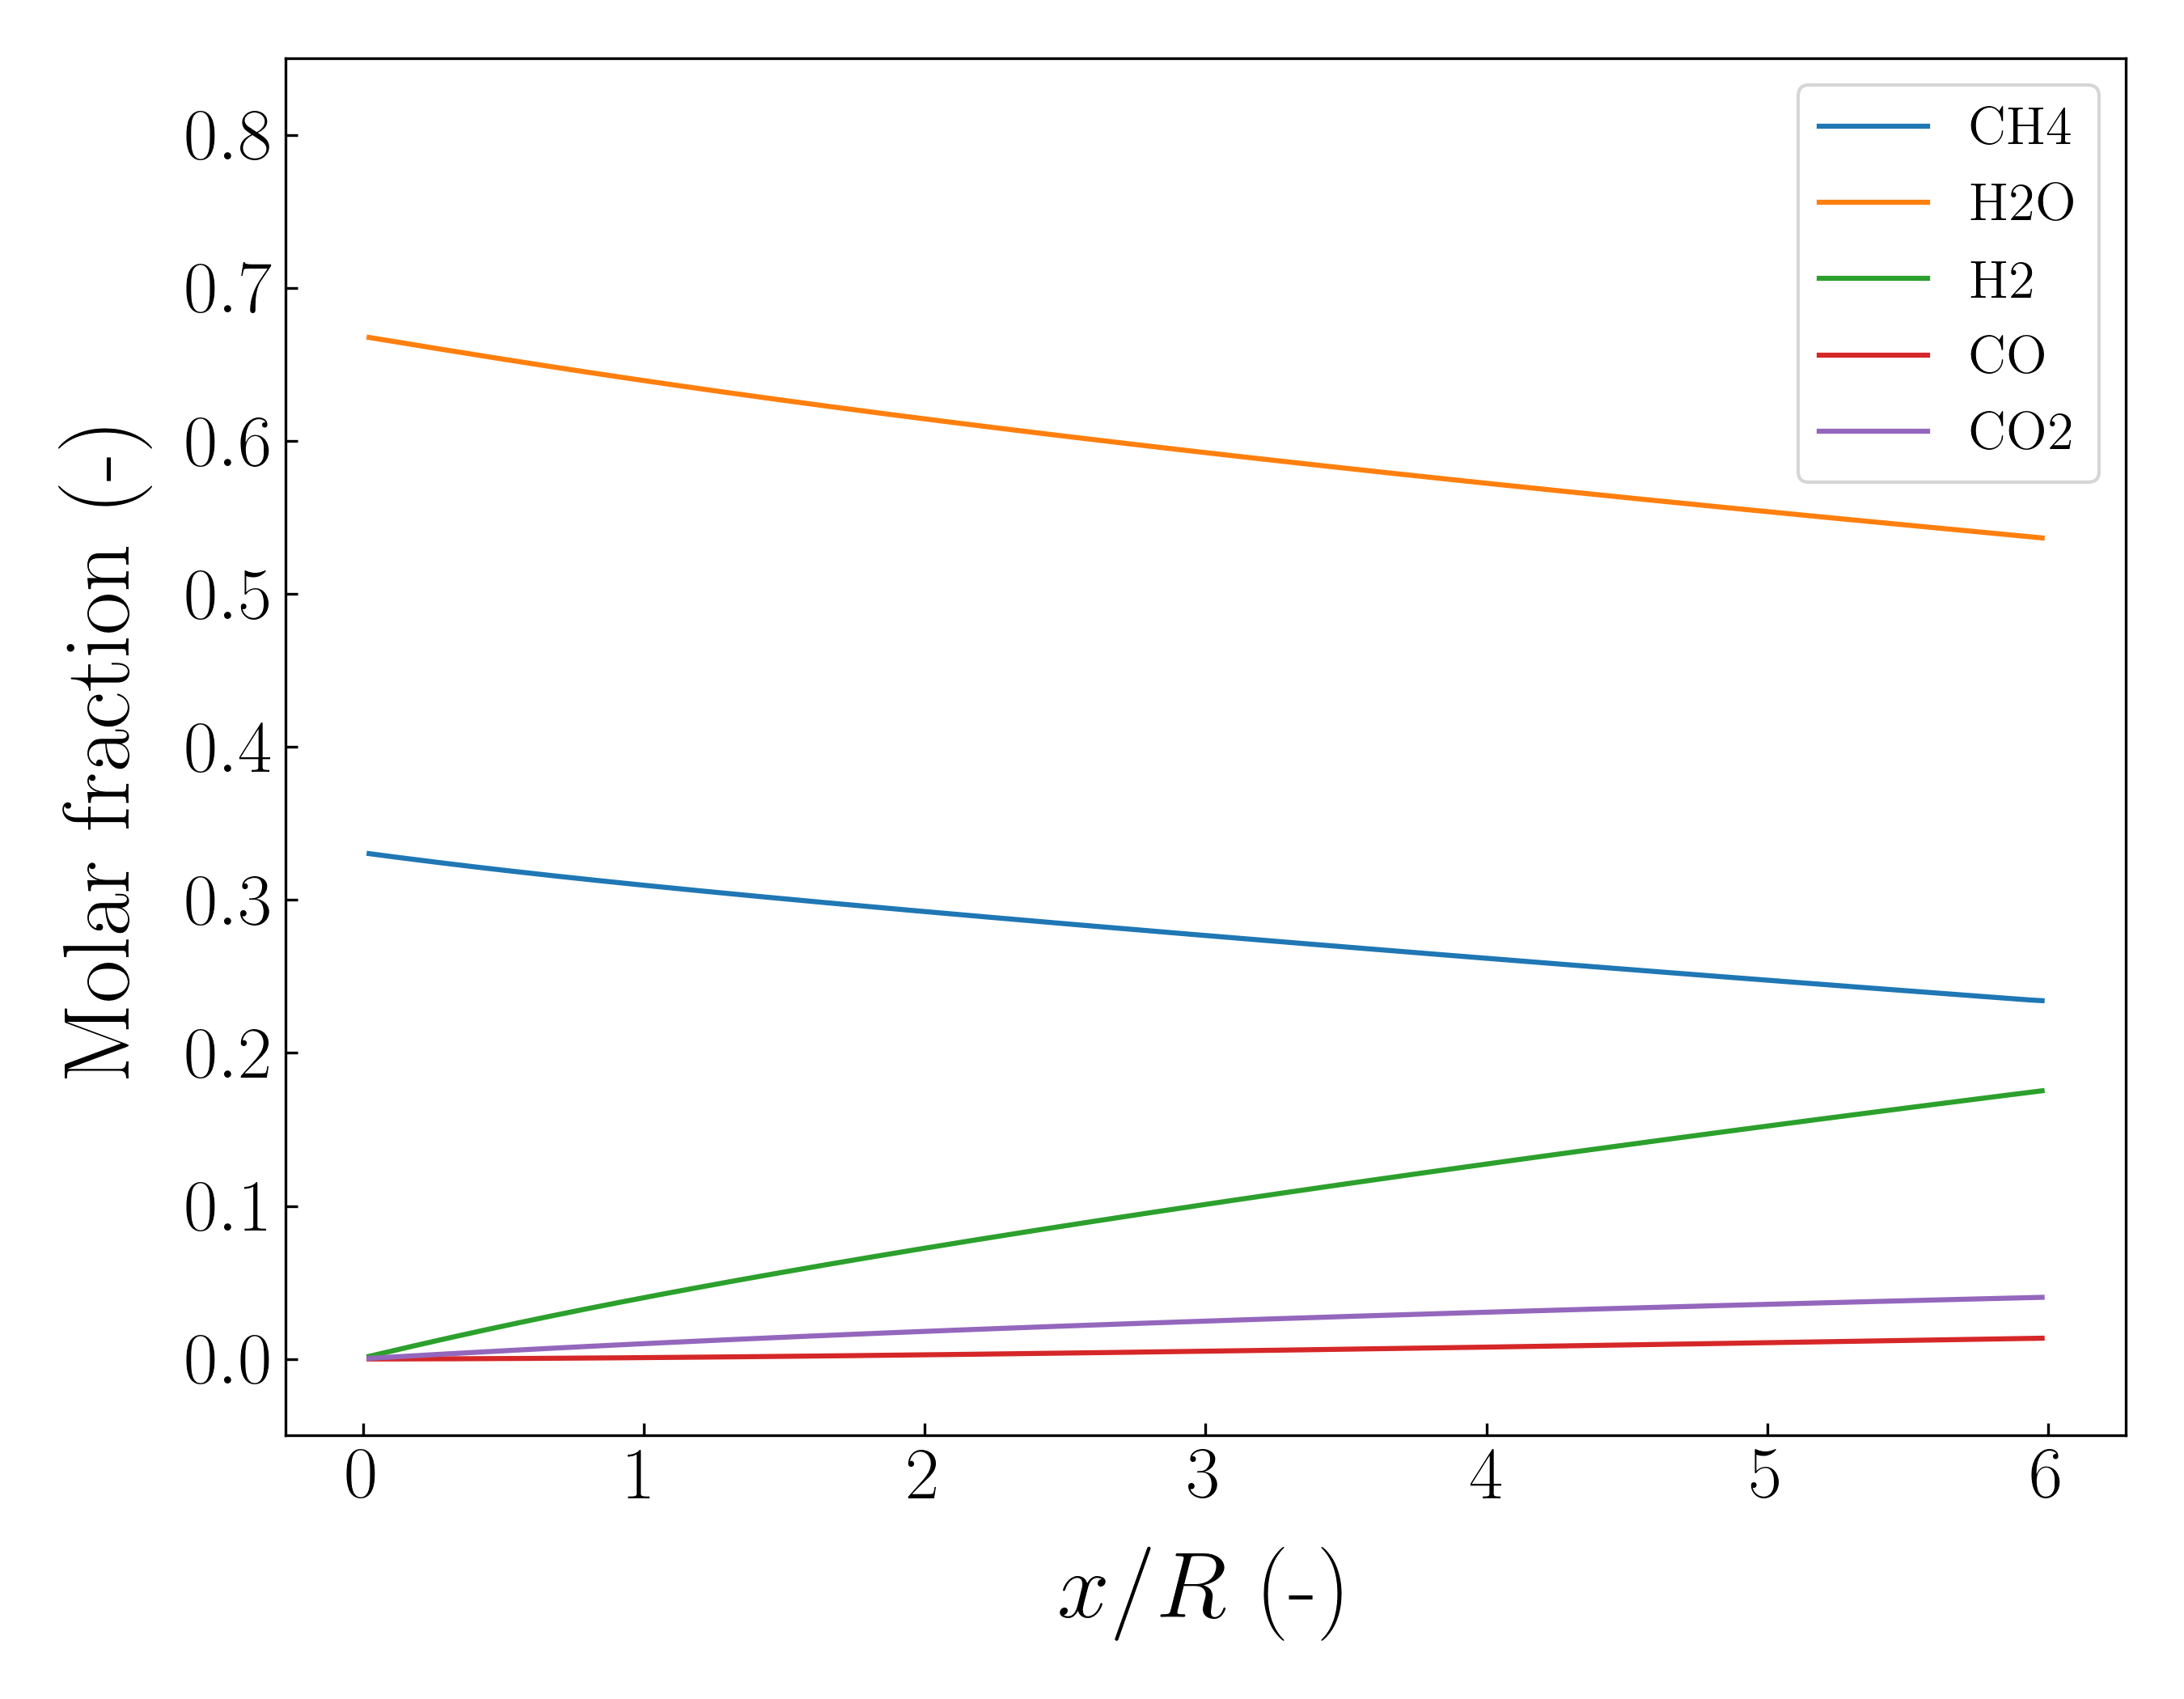
\includegraphics[width=80mm]{results/5/50C_50T/GEN15-AVG.png}
\caption{\label{fig:5R5050G15-avg} Strategy I - Radius-averaged molar fractions - 15$^{\rm{th}}$ generation ($w_{\rm{CH_4}} = 0.5, w_T = 0.5$, $T_{\rm{in}}$ = 900 K, $u_{\rm{in}}$ = 0.15 m s$^{-1}$, $SC$ = 2.0)}
\end{figure}

\begin{figure}[h!]
\centering
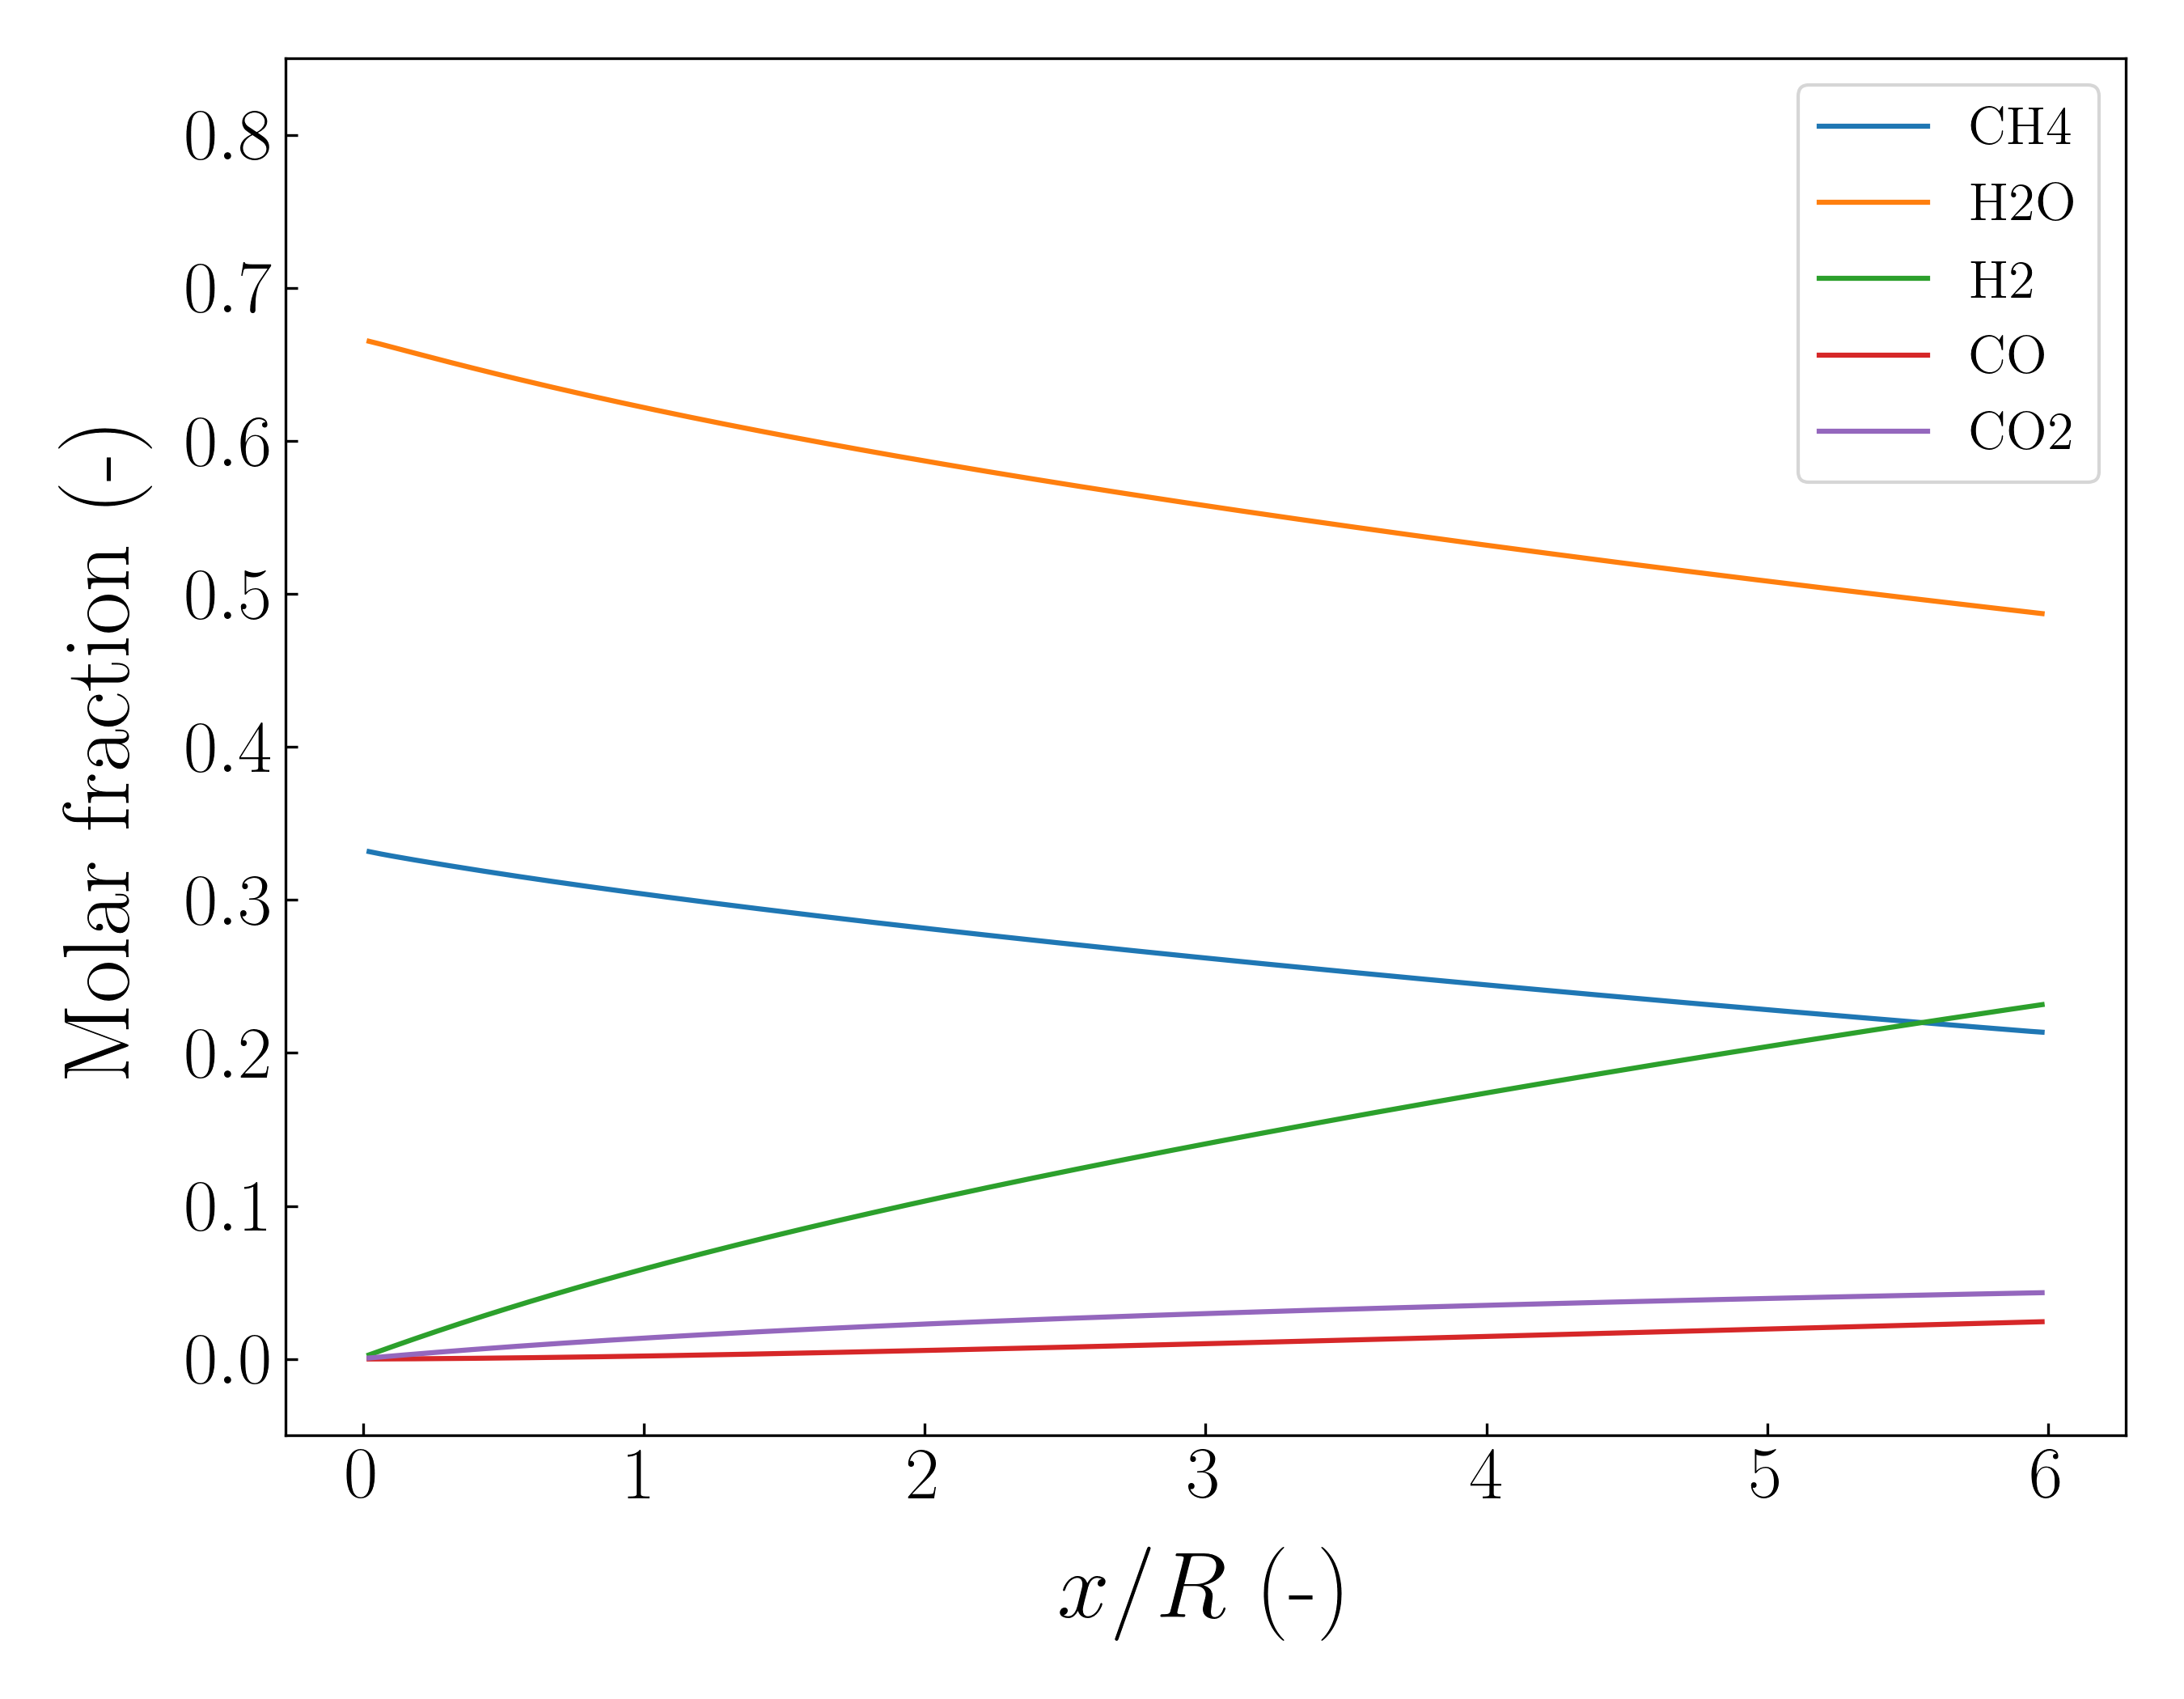
\includegraphics[width=80mm]{results/5/50C_50T/GEN30-AVG.png}
\caption{\label{fig:5R5050G30-avg} Strategy I - Radius-averaged molar fractions -  30$^{\rm{th}}$ generation ($w_{\rm{CH_4}} = 0.5, w_T = 0.5$, $T_{\rm{in}}$ = 900 K, $u_{\rm{in}}$ = 0.15 m s$^{-1}$, $SC$ = 2.0)}
\end{figure}

\begin{figure}[h!]
\centering
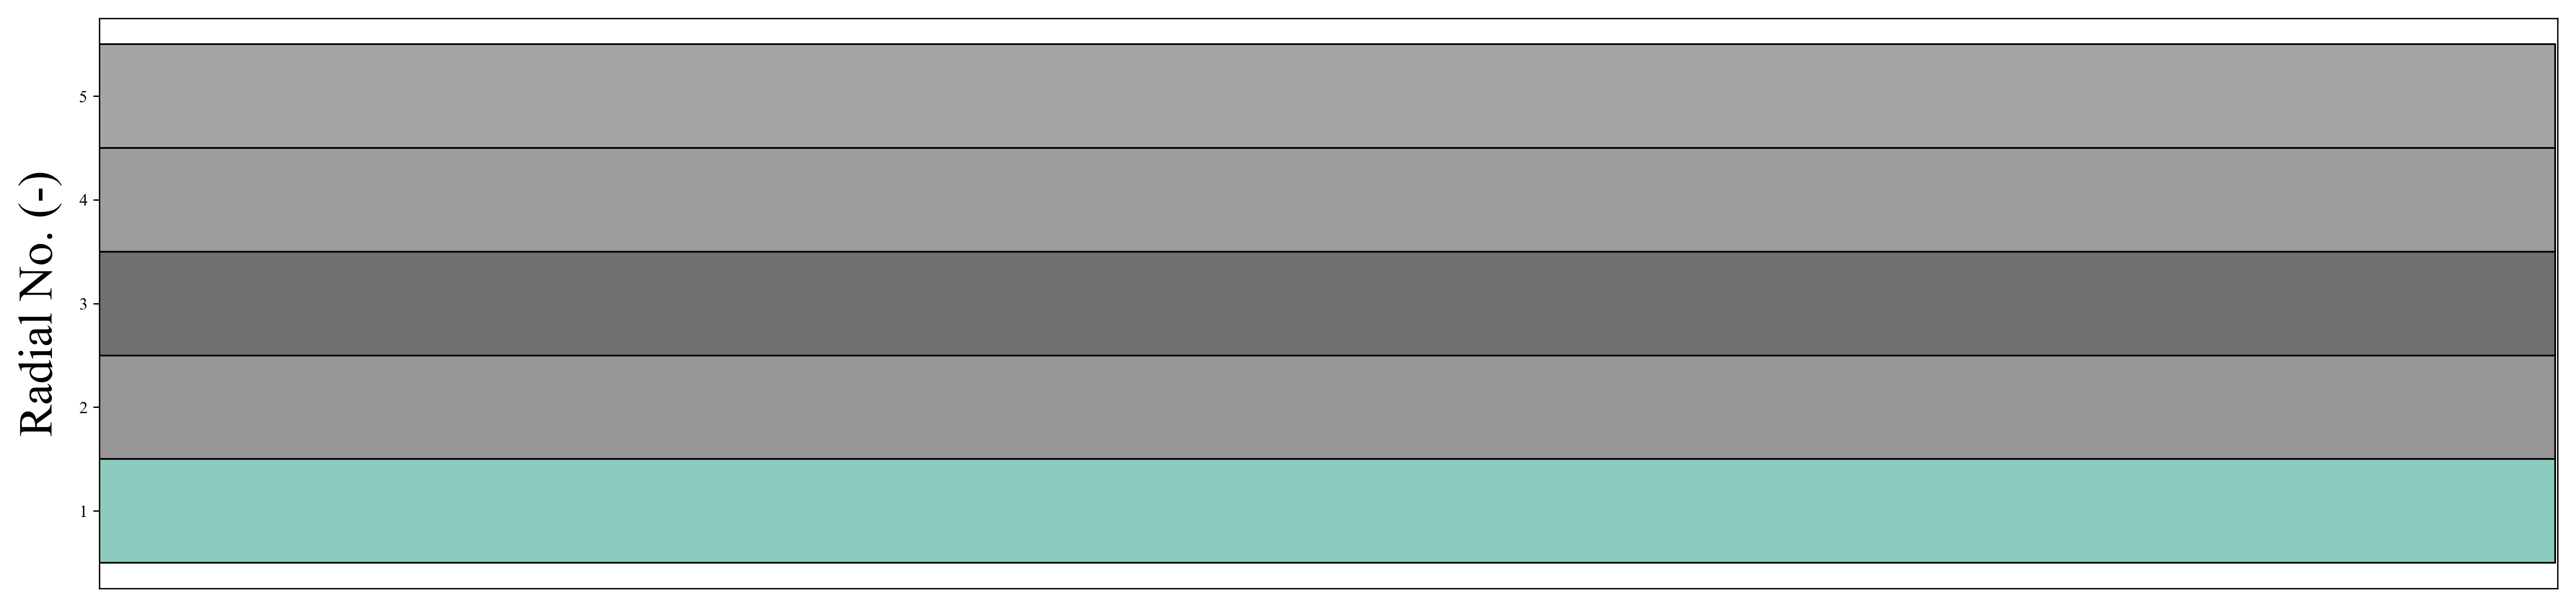
\includegraphics[width=120mm]{results/segments/5seg/50C50T/seg.png}
\caption{\label{fig:30L6040G1-TField} Strategy I - Segments distribution for 30$^{\rm{th}}$ generation ($w_{\rm{CH_4}} = 0.5, w_T = 0.5$, $T_{\rm{in}}$ = 900 K, $u_{\rm{in}}$ = 0.15 m s$^{-1}$, $SC$ = 2.0)}
\end{figure}

%\begin{figure}[h!]
%\centering
%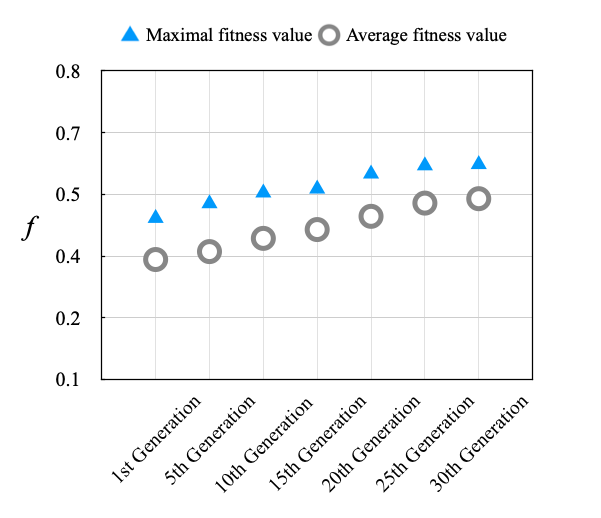
\includegraphics[width=100mm]{results/5/50C_50T.png}
%\caption{\label{fig:5R5050G-fitness} Strategy I - Fitness analysis throughout successive populations ($w_{\rm{CH_4}} = 0.5, w_T = 0.5$, $T_{\rm{in}}$ = 900 K, $u_{\rm{in}}$ = 0.15 m s$^{-1}$, $SC$ = 2.0)}
%\end{figure}


\clearpage



\paragraph{Thermal fitness 40 \%, methane conversion 60 \%} \hspace{0pt} \\
\noindent 


\begin{figure}[h!]
\centering
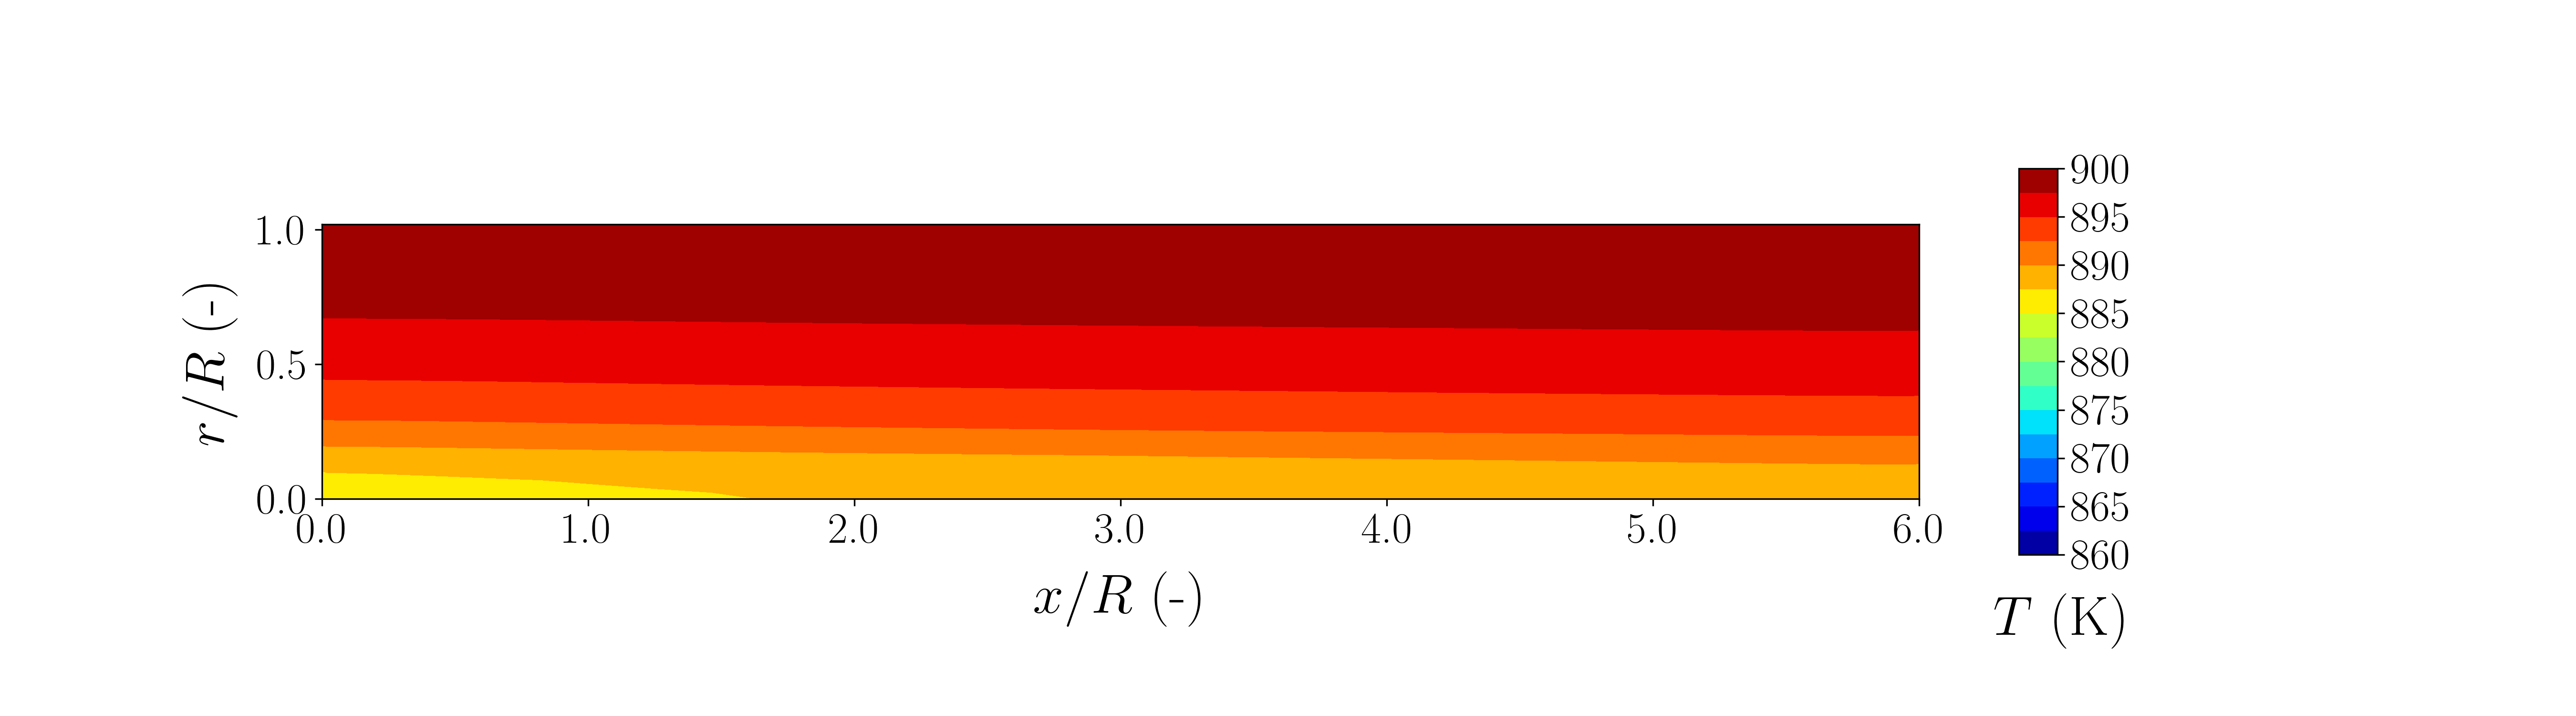
\includegraphics[width=190mm]{results/5/60C_40T/GEN1-TFIELD.png}
\caption{\label{fig:5R6040G1-TField} Strategy I - Temperature field distribution - 1$^{\rm{st}}$ generation ($w_{\rm{CH_4}} = 0.6, w_T = 0.4$, $T_{\rm{in}}$ = 900 K, $u_{\rm{in}}$ = 0.15 m s$^{-1}$, $SC$ = 2.0)}
\end{figure}

\begin{figure}[h!]
\centering
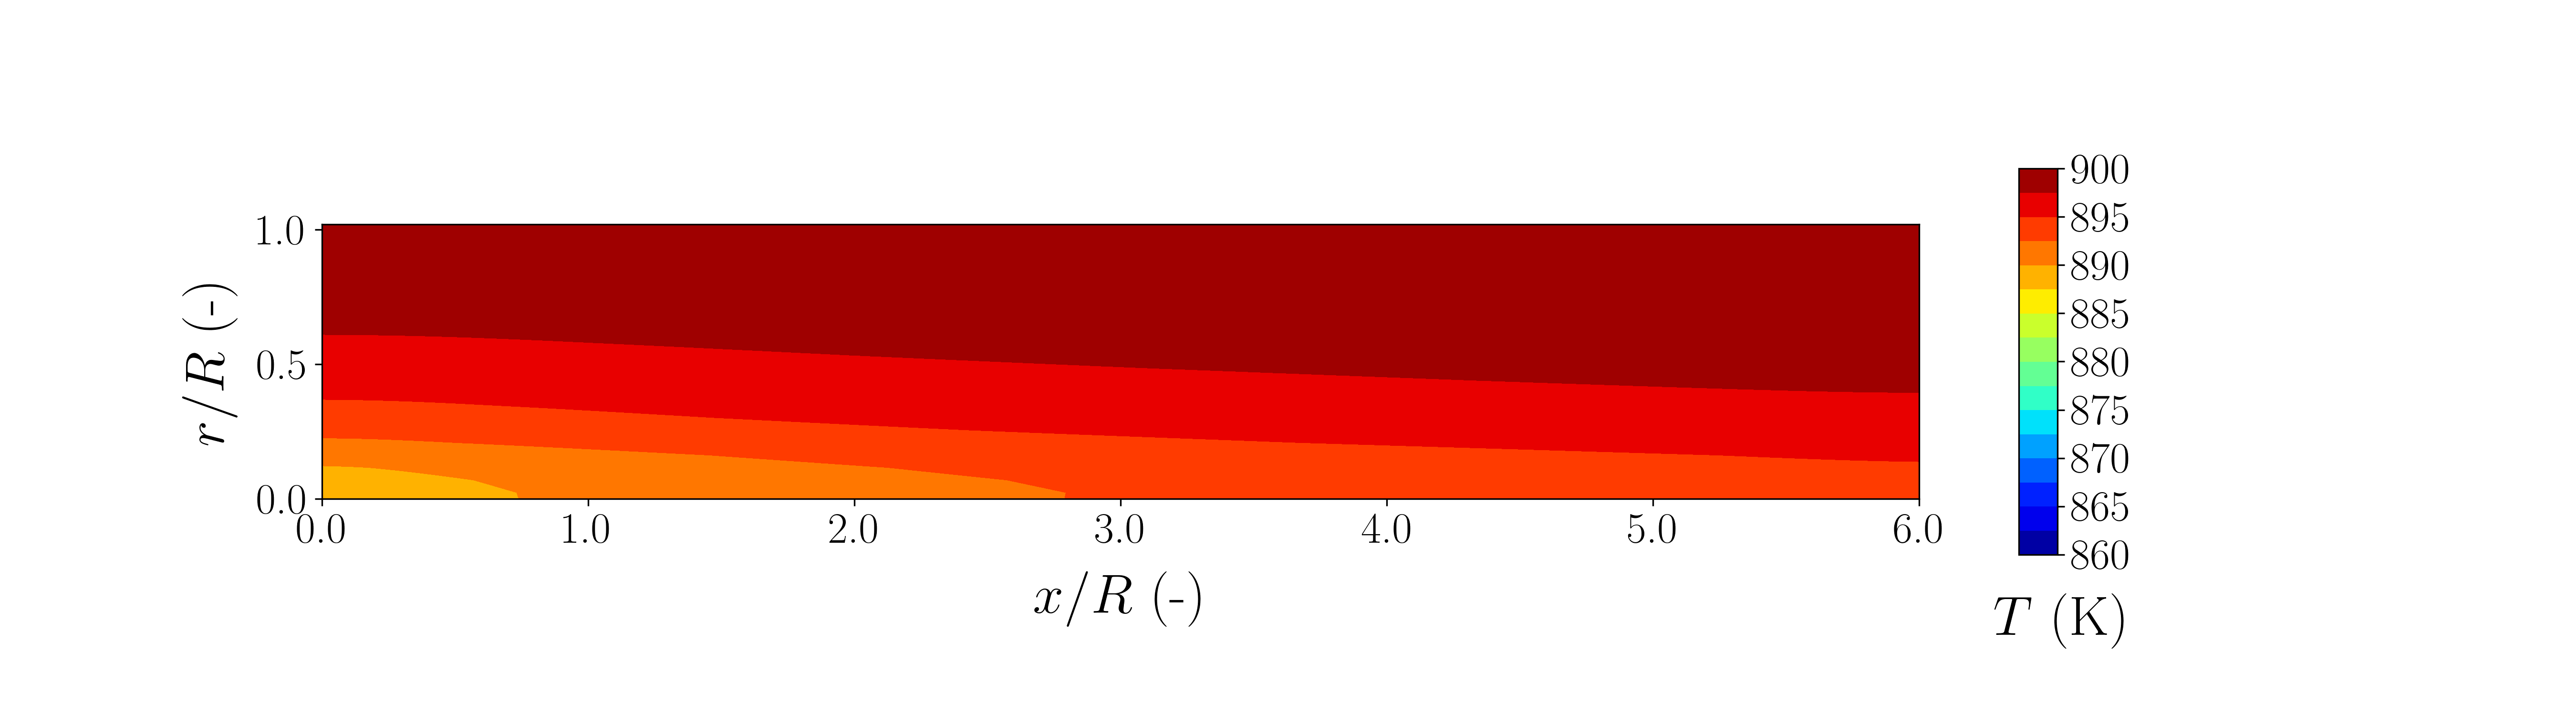
\includegraphics[width=190mm]{results/5/60C_40T/GEN15-TFIELD.png}
\caption{\label{fig:5R6040G15-TField} Strategy I - Temperature field distribution - 15$^{\rm{th}}$ generation ($w_{\rm{CH_4}} = 0.6, w_T = 0.4$, $T_{\rm{in}}$ = 900 K, $u_{\rm{in}}$ = 0.15 m s$^{-1}$, $SC$ = 2.0)}
\end{figure}

\begin{figure}[h!]
\centering
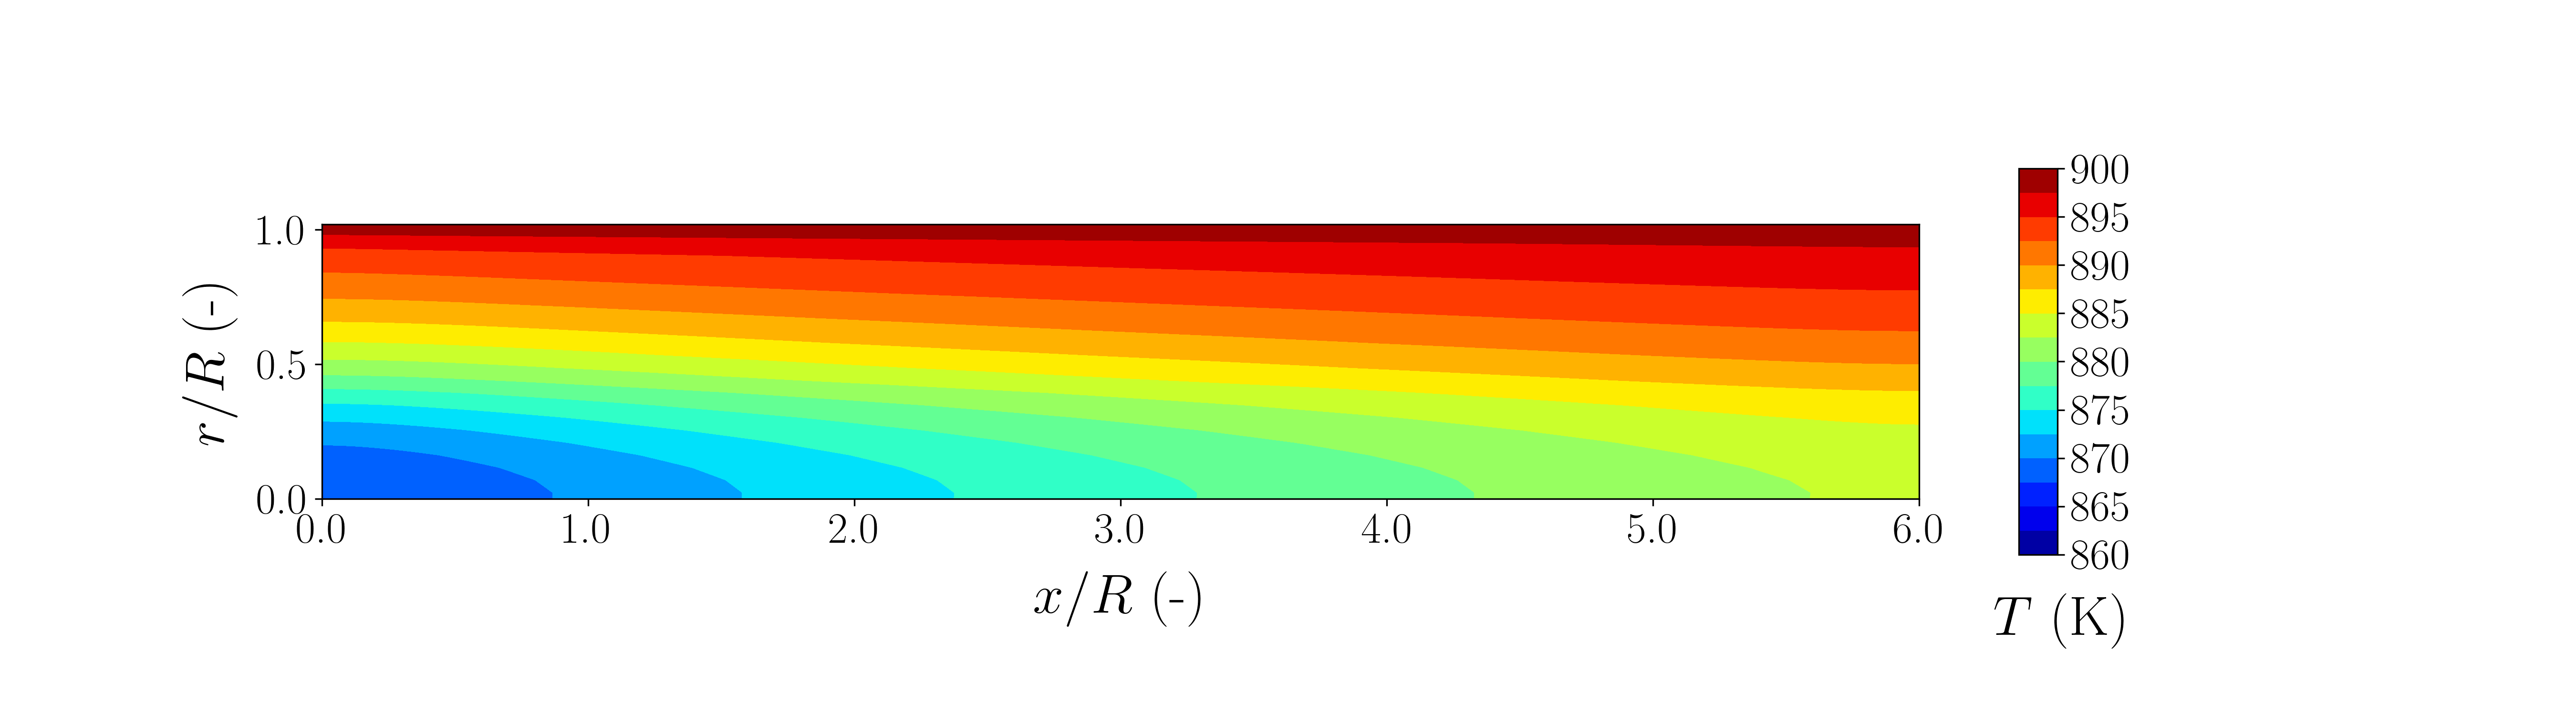
\includegraphics[width=190mm]{results/5/60C_40T/GEN30-TFIELD.png}
\caption{\label{fig:5R6040G30-TField} Strategy I - Temperature field distribution - 30$^{\rm{th}}$ generation ($w_{\rm{CH_4}} = 0.6, w_T = 0.4$, $T_{\rm{in}}$ = 900 K, $u_{\rm{in}}$ = 0.15 m s$^{-1}$, $SC$ = 2.0)}
\end{figure}


\begin{figure}[h!]
\centering
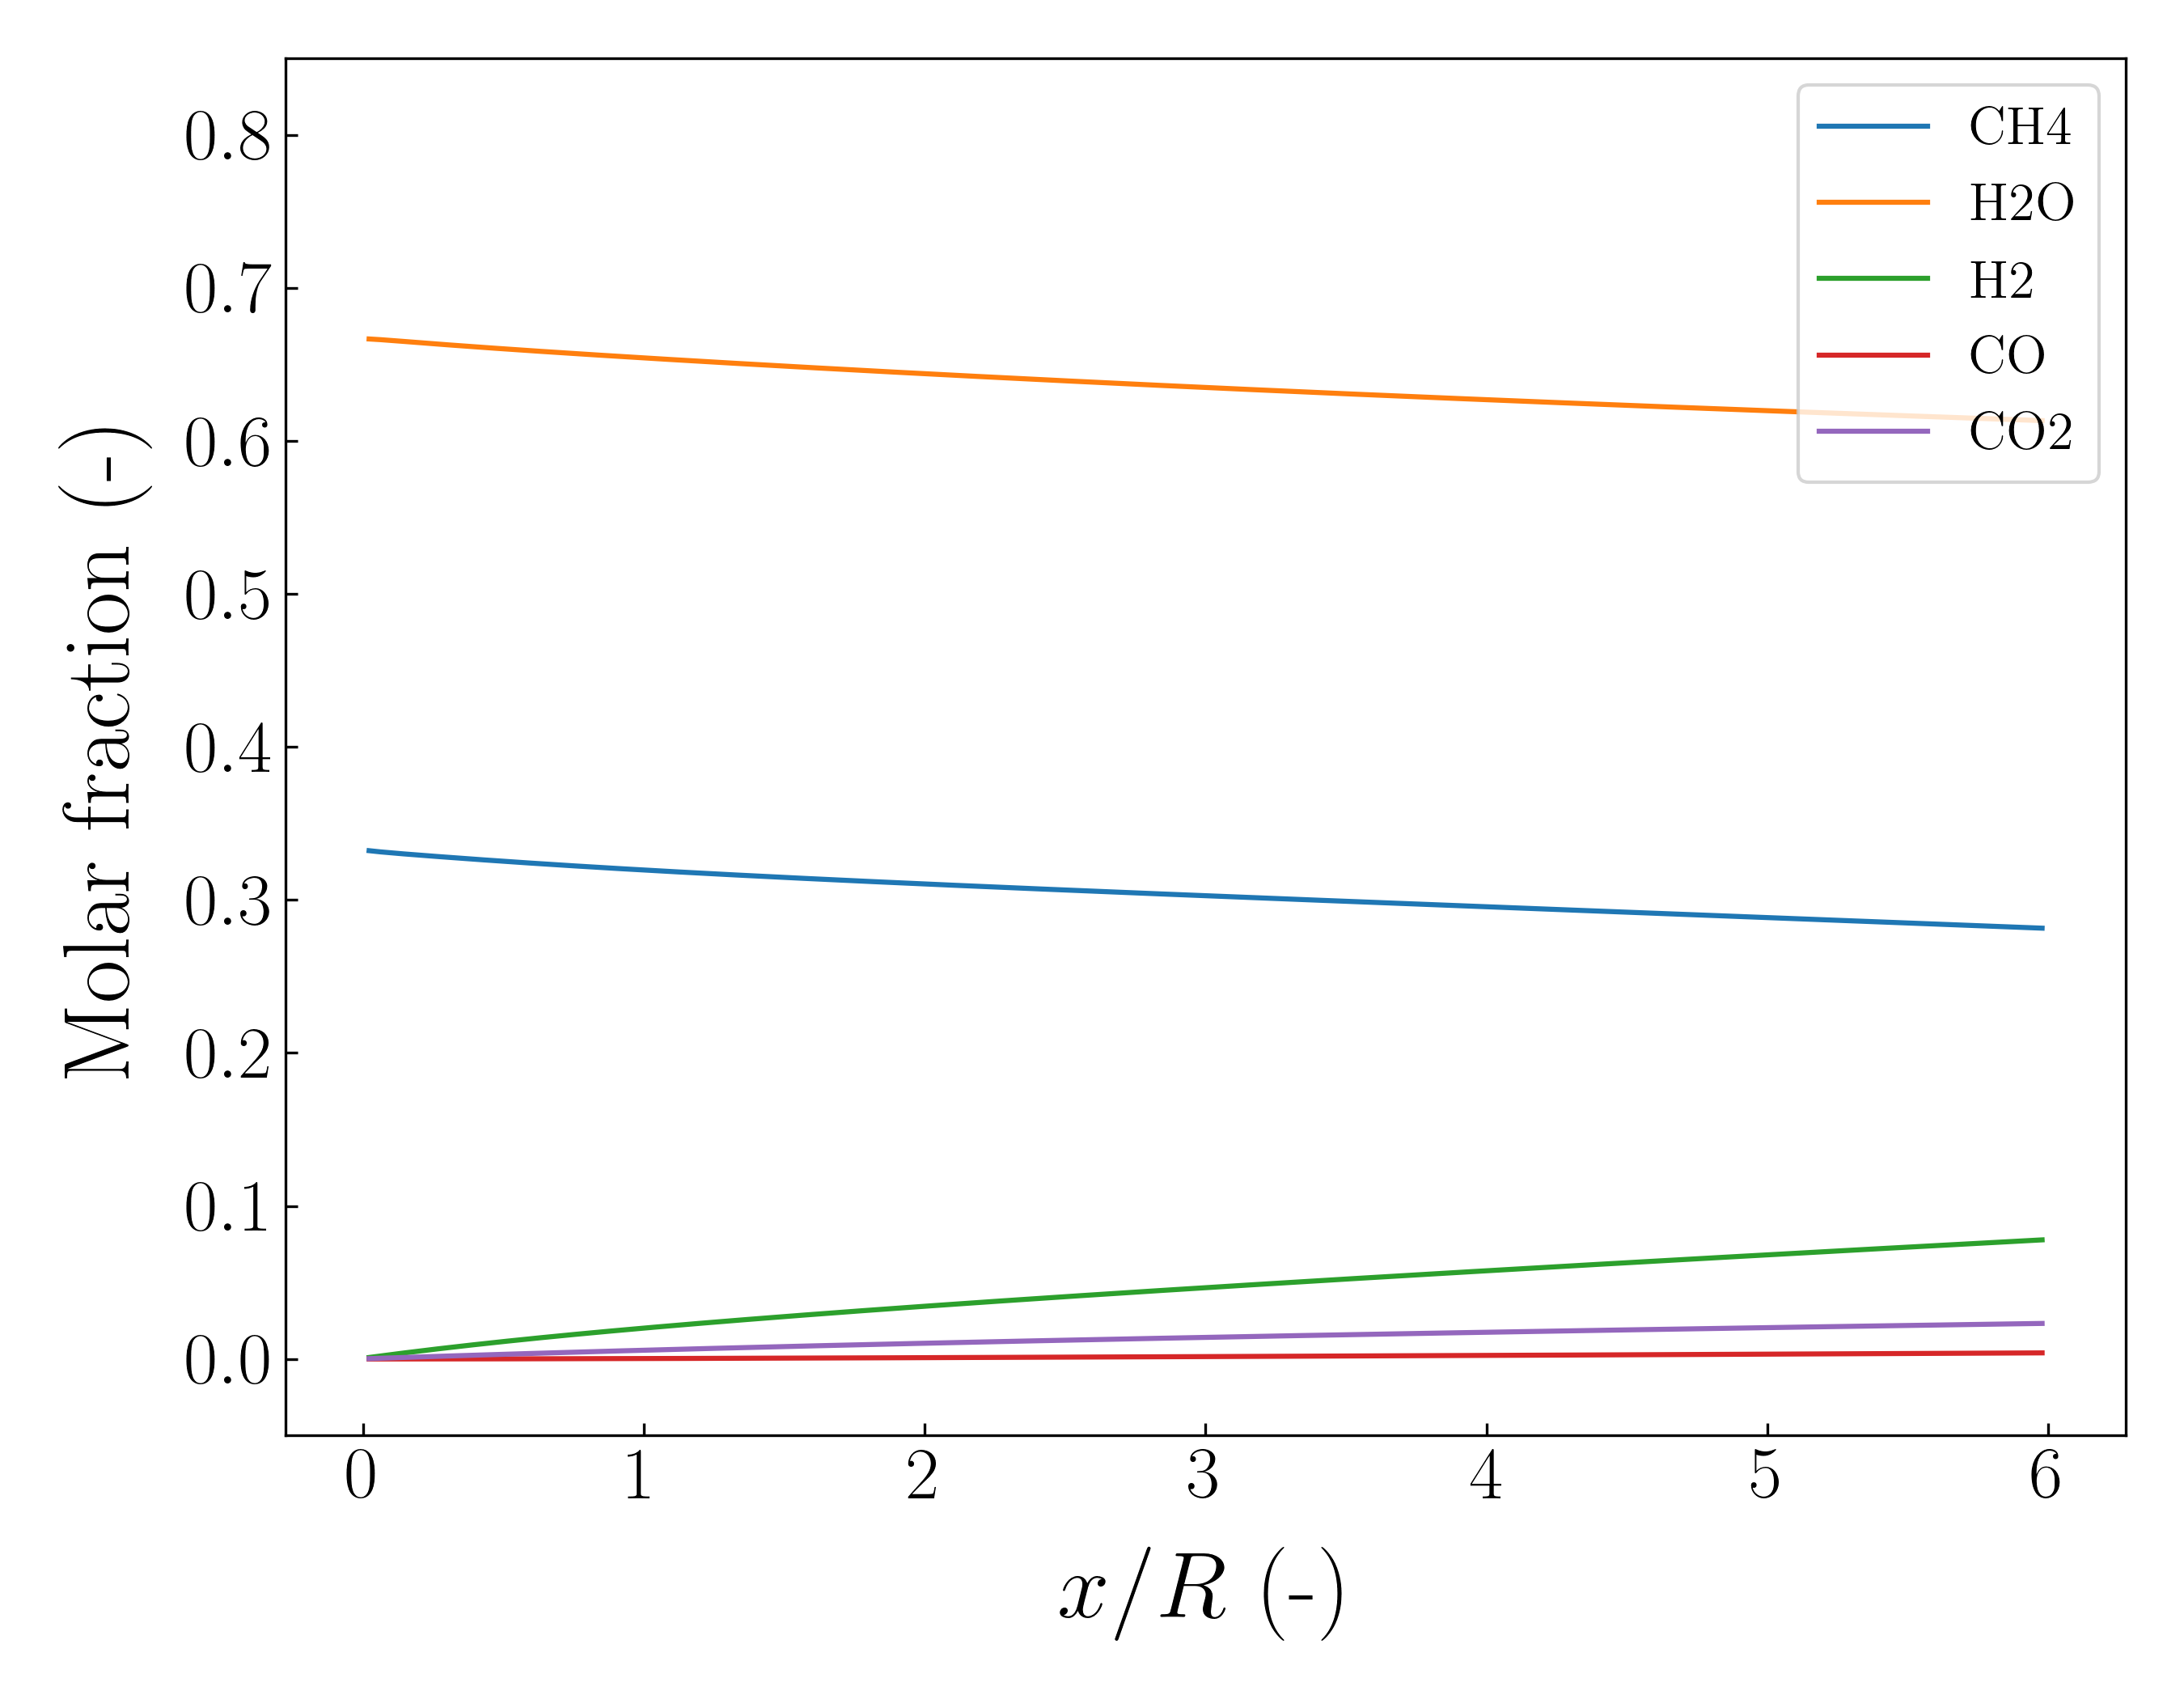
\includegraphics[width=80mm]{results/5/60C_40T/GEN1-AVG.png}
\caption{\label{fig:5R6040G1-avg} Strategy I - Radius-averaged molar fractions - 1$^{\rm{st}}$ generation ($w_{\rm{CH_4}} = 0.6, w_T = 0.4$, $T_{\rm{in}}$ = 900 K, $u_{\rm{in}}$ = 0.15 m s$^{-1}$, $SC$ = 2.0)}
\end{figure}

\begin{figure}[h!]
\centering
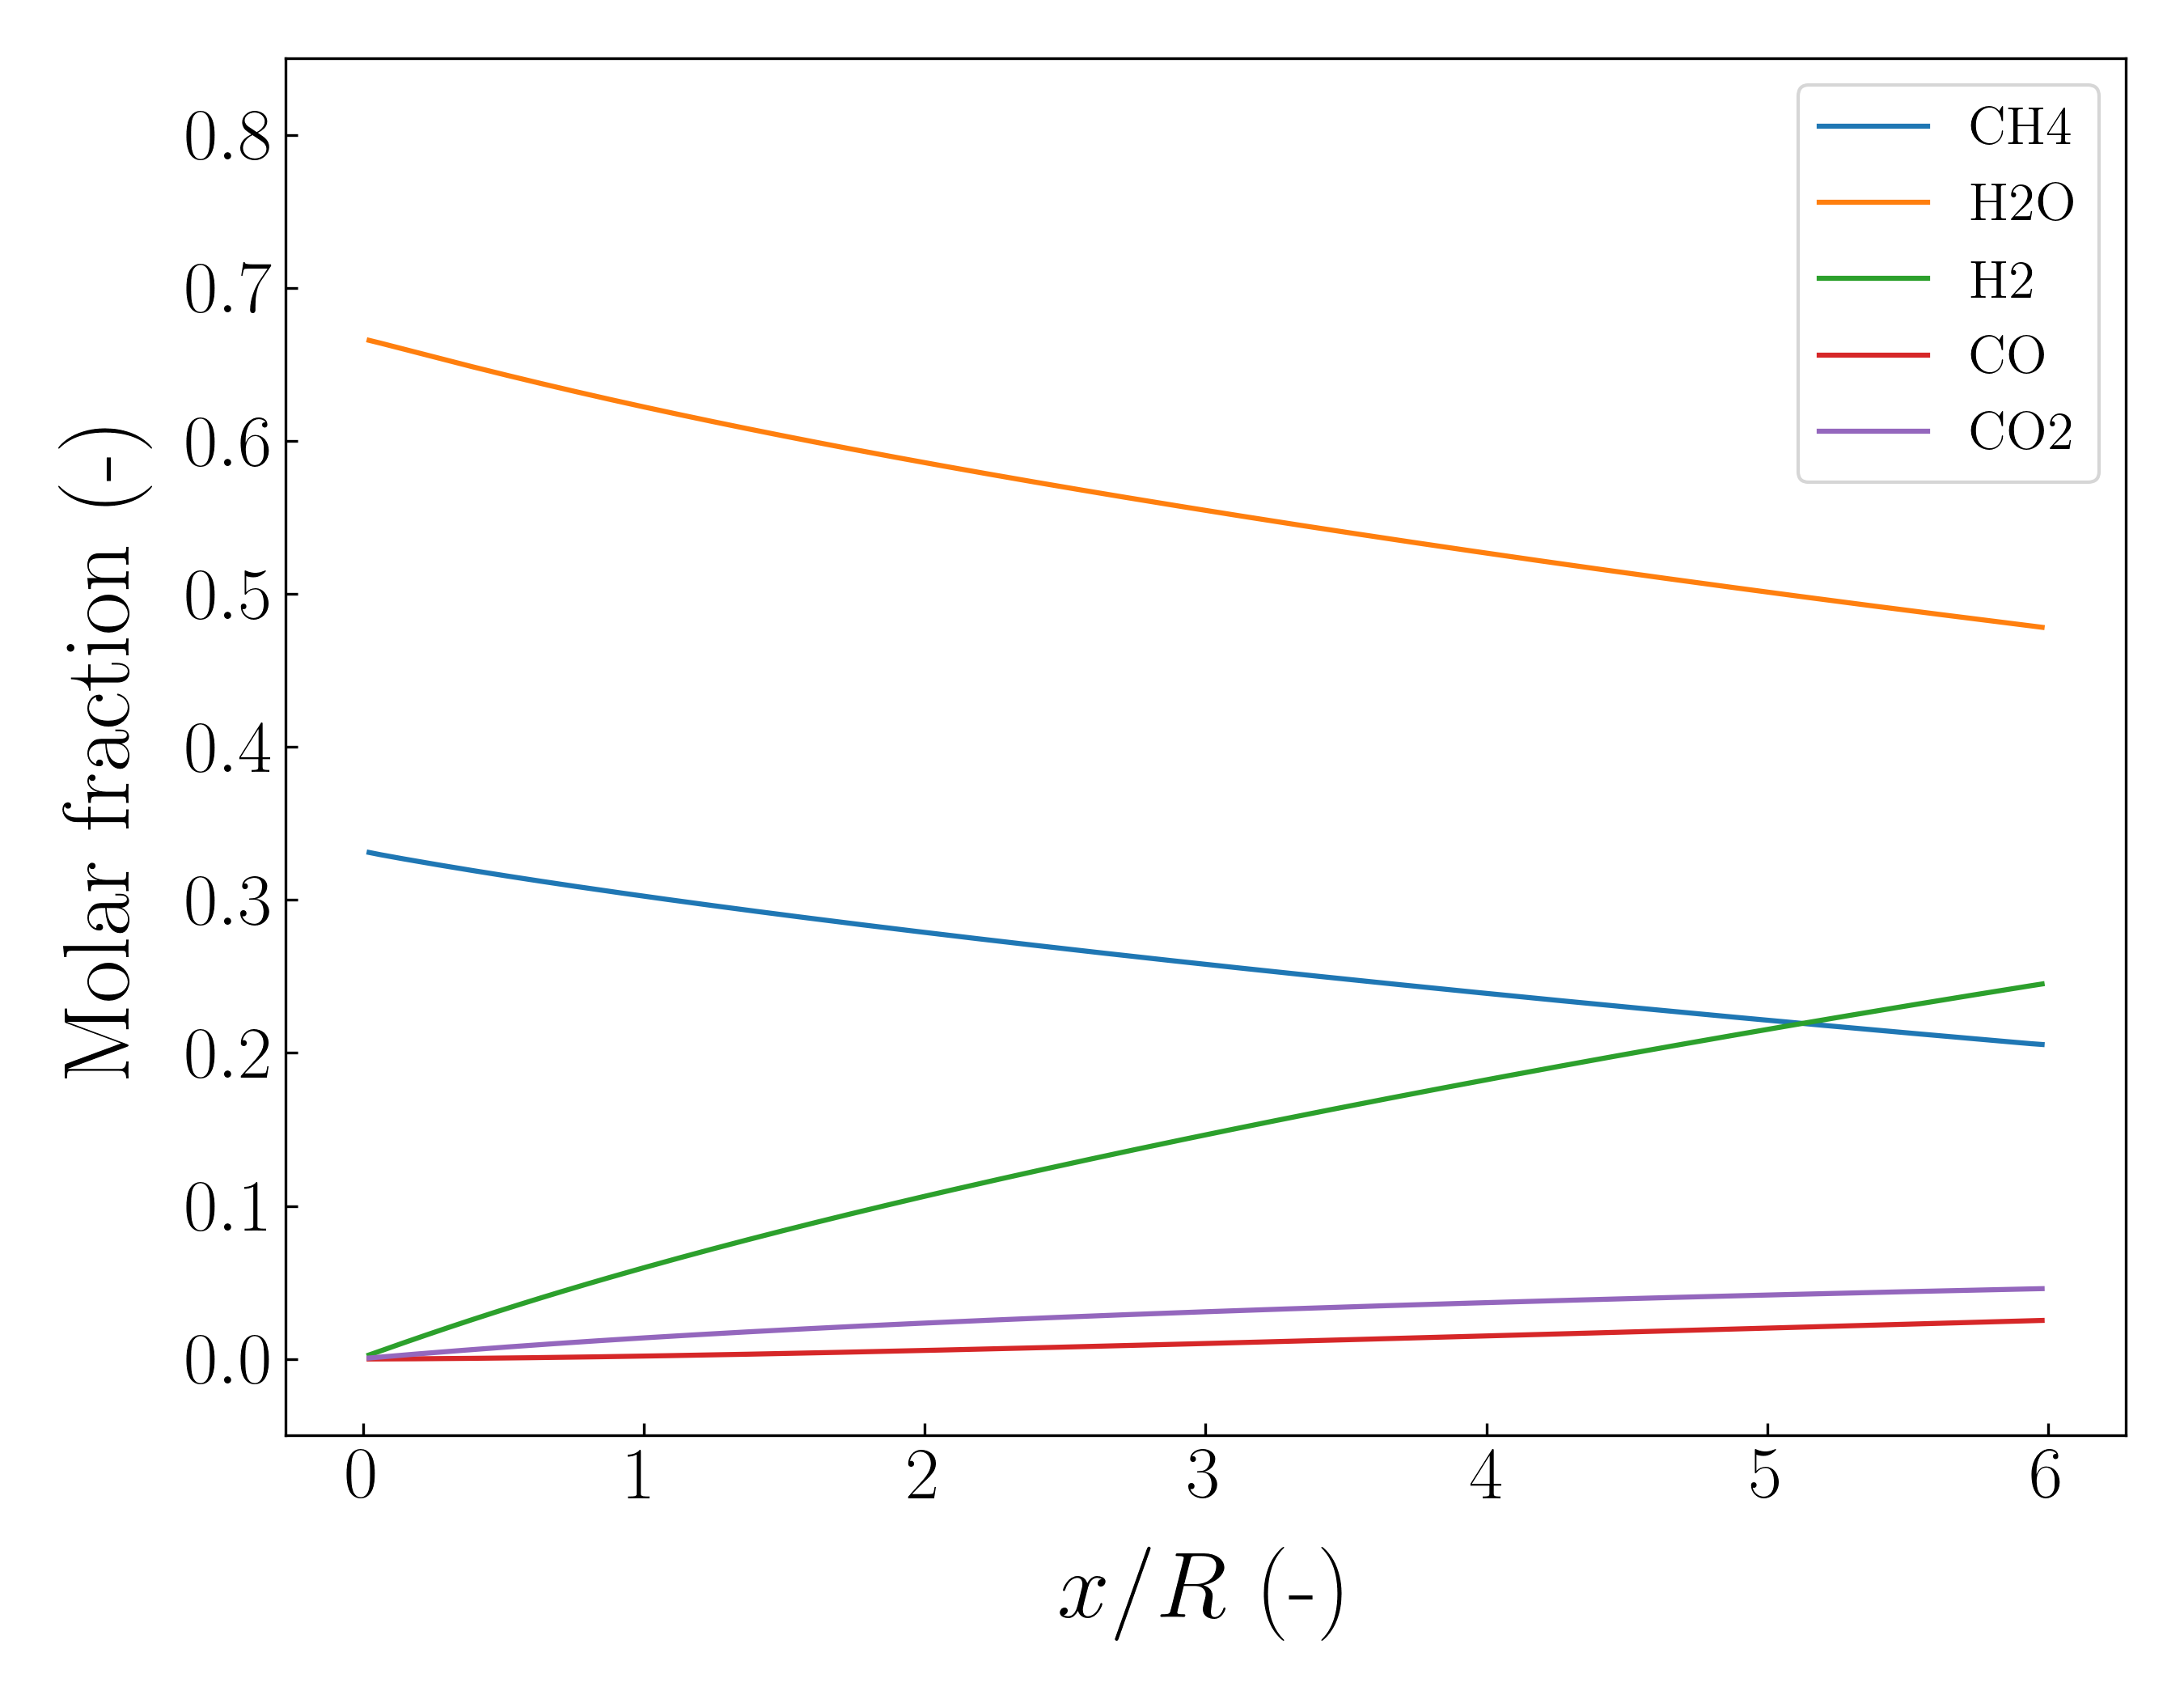
\includegraphics[width=80mm]{results/5/60C_40T/GEN15-AVG.png}
\caption{\label{fig:5R6040G15-avg} Strategy I - Radius-averaged molar fractions - 15$^{\rm{th}}$ generation ($w_{\rm{CH_4}} = 0.6, w_T = 0.4$, $T_{\rm{in}}$ = 900 K, $u_{\rm{in}}$ = 0.15 m s$^{-1}$, $SC$ = 2.0)}
\end{figure}

\begin{figure}[h!]
\centering
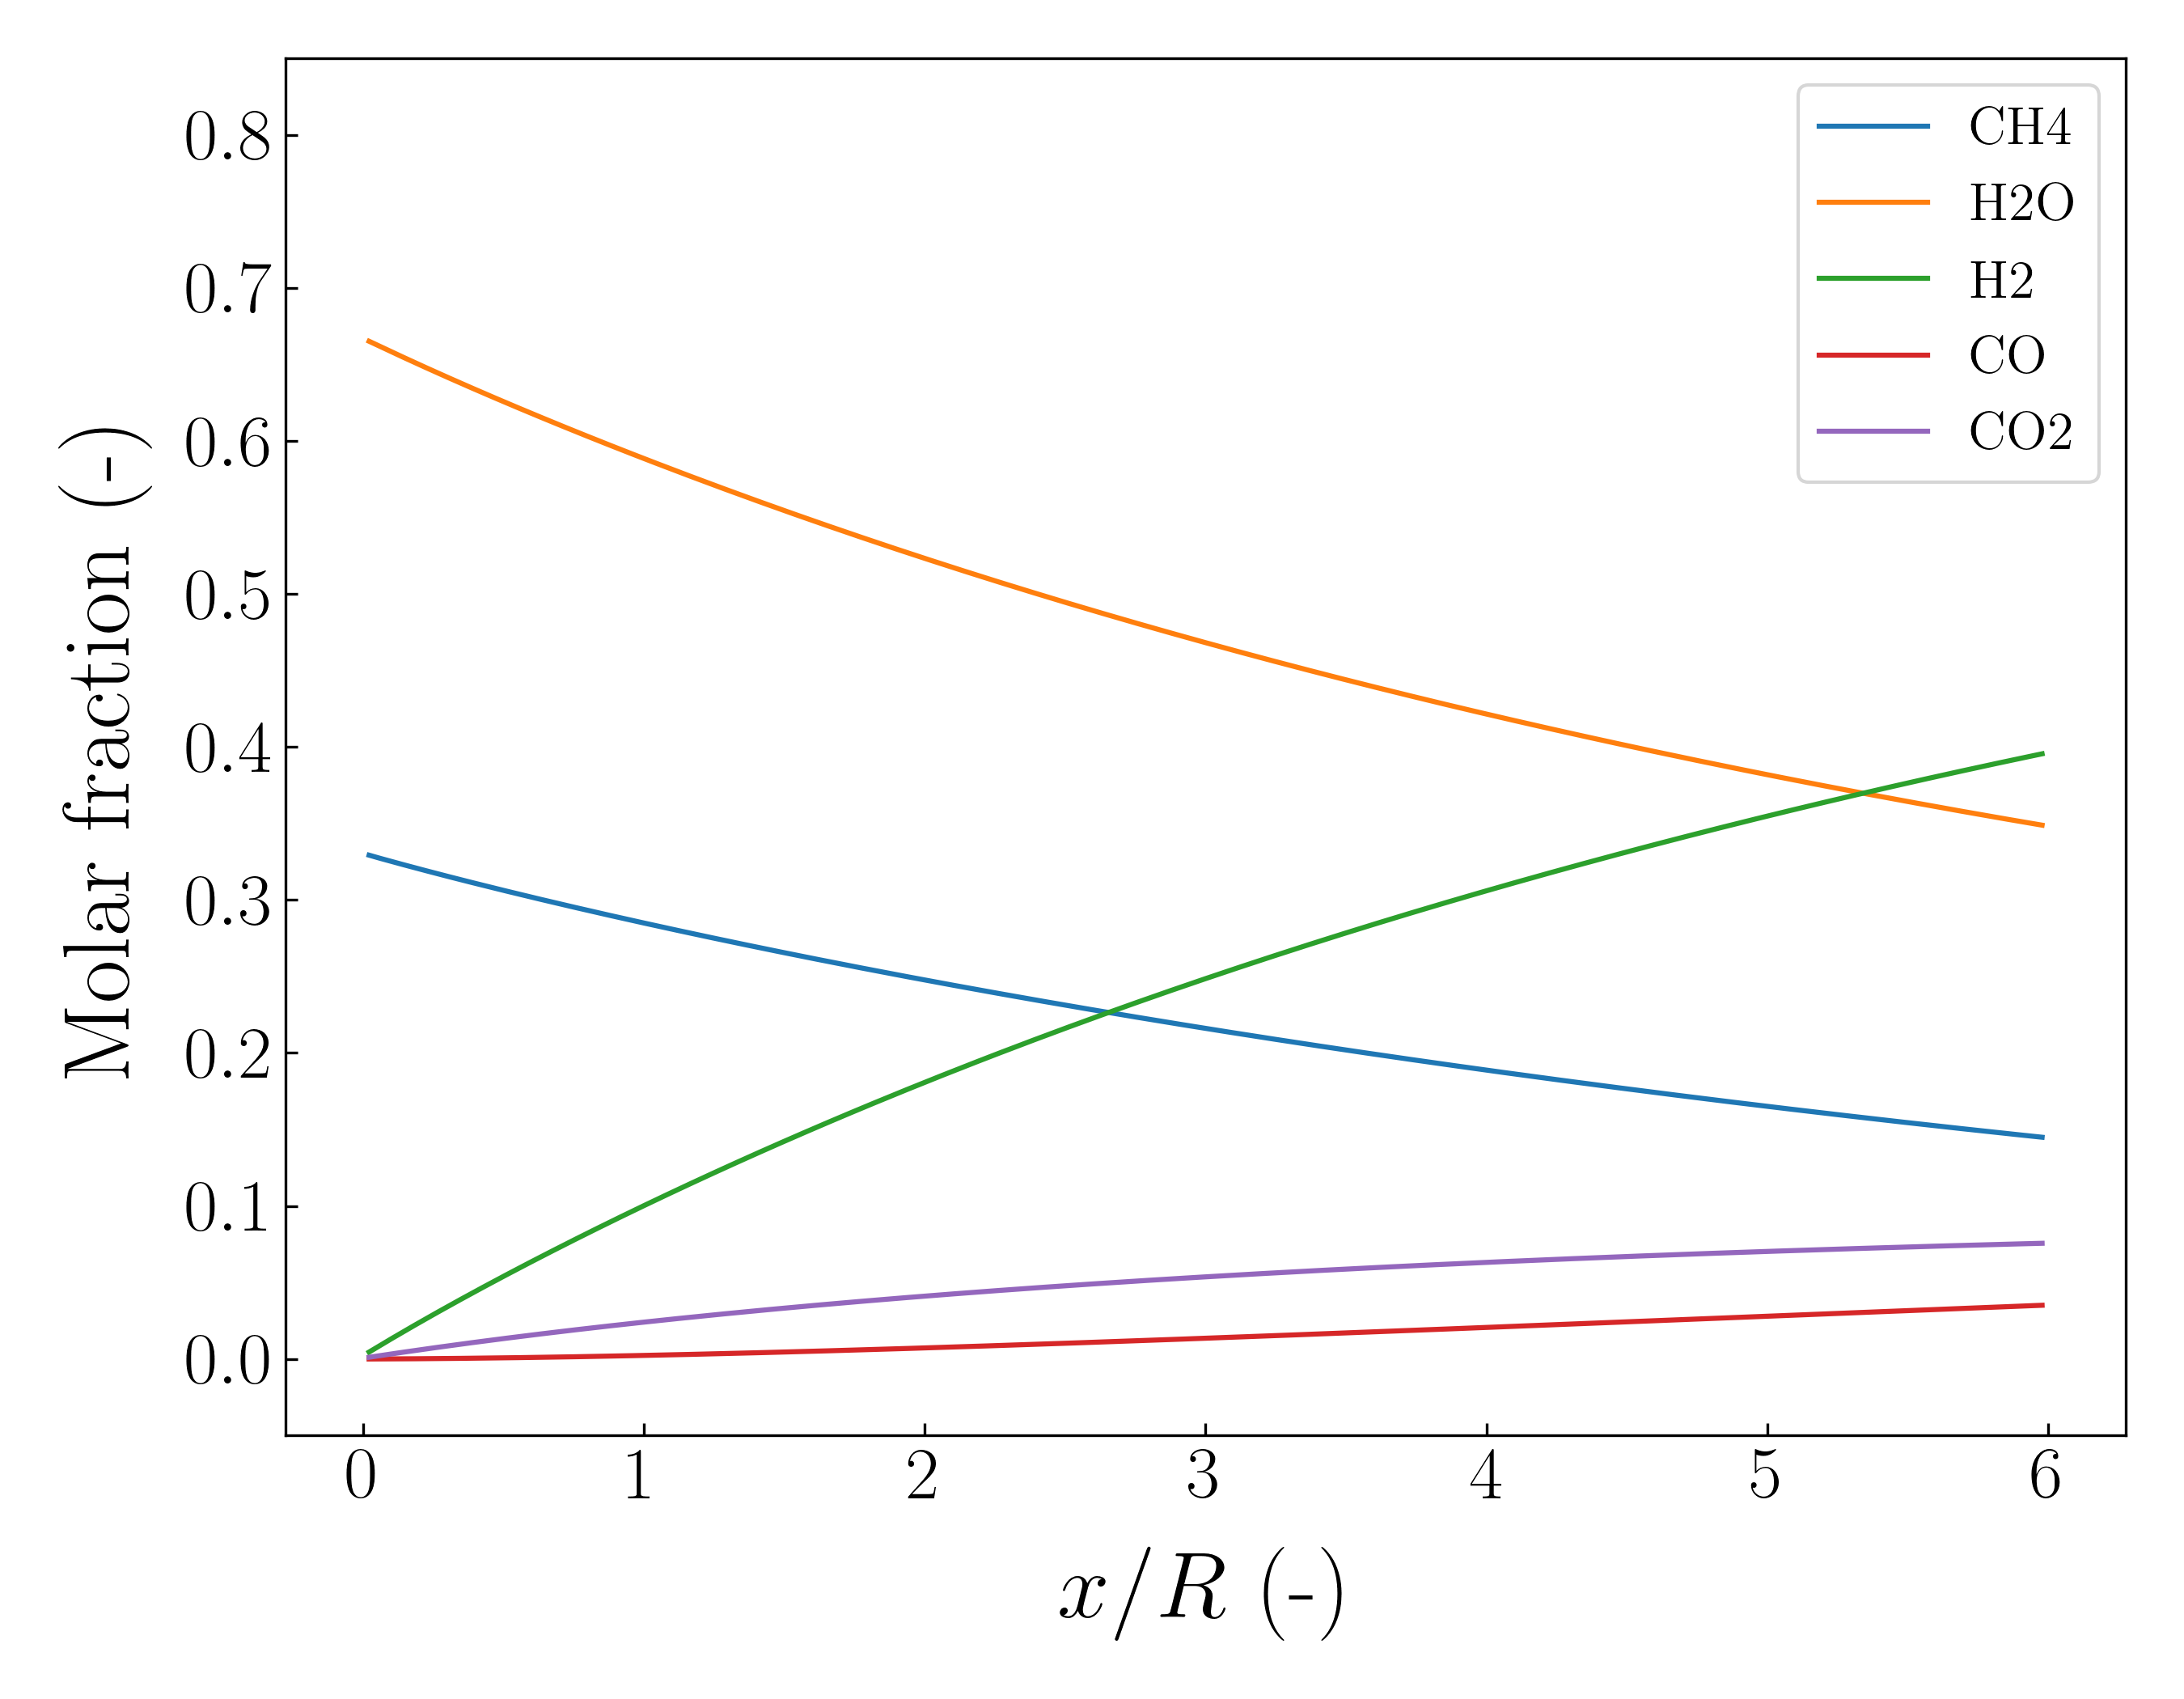
\includegraphics[width=80mm]{results/5/60C_40T/GEN30-AVG.png}
\caption{\label{fig:5R6040G30-avg} Strategy I - Radius-averaged molar fractions -  30$^{\rm{th}}$ generation ($w_{\rm{CH_4}} = 0.6, w_T = 0.4$, $T_{\rm{in}}$ = 900 K, $u_{\rm{in}}$ = 0.15 m s$^{-1}$, $SC$ = 2.0)}
\end{figure}

\begin{figure}[h!]
\centering
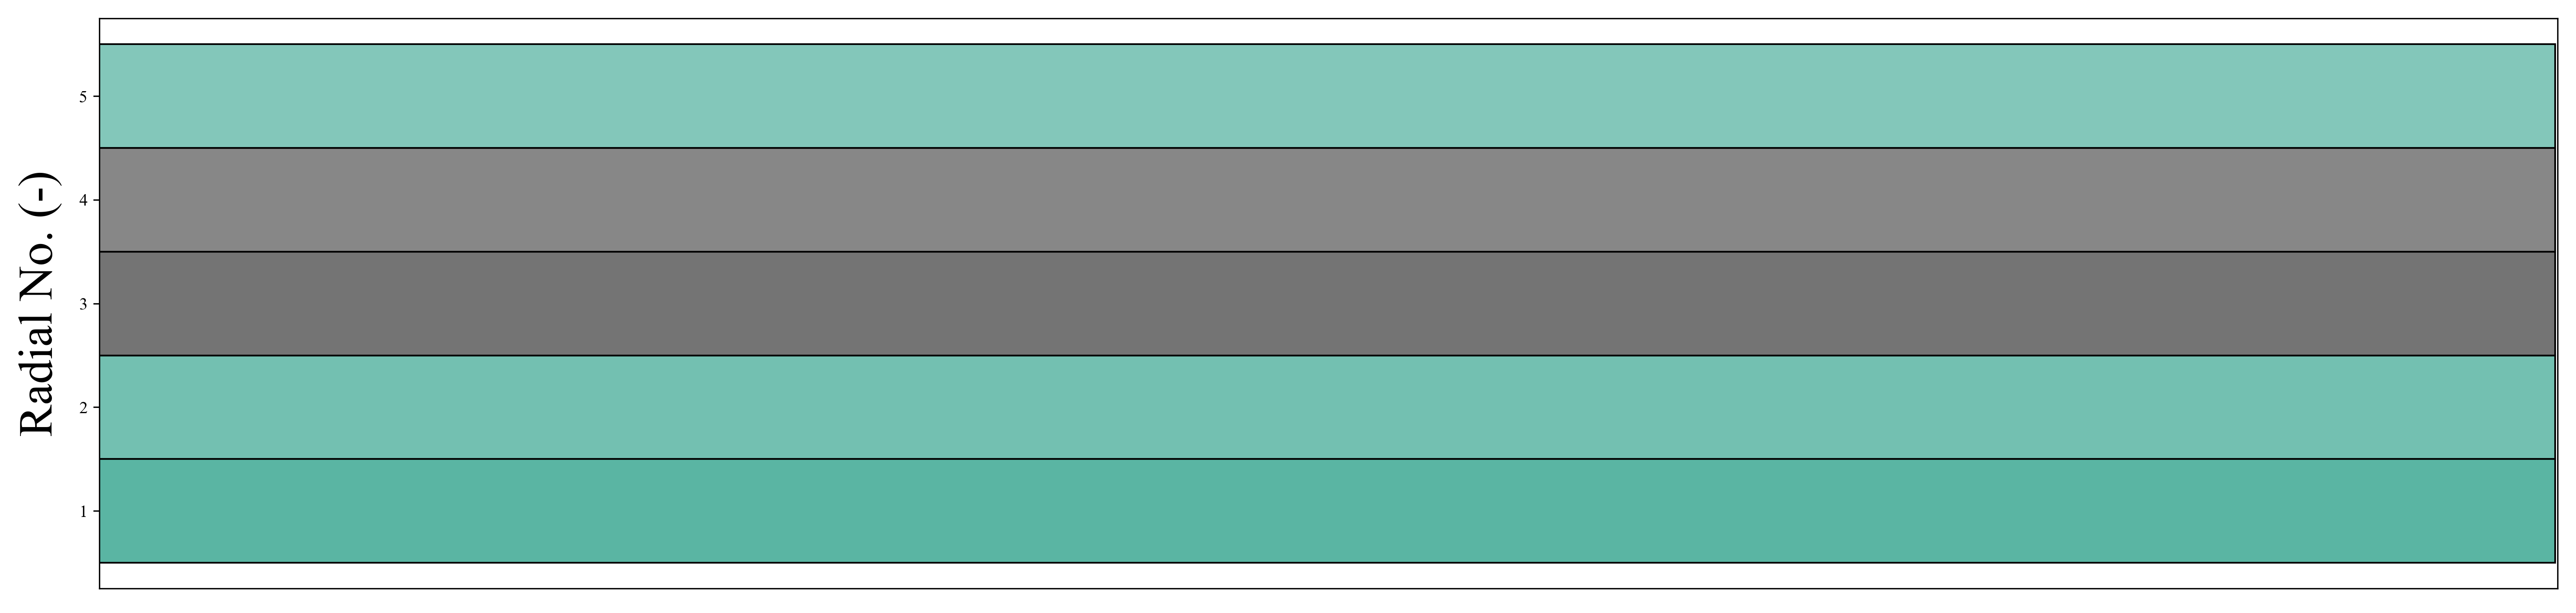
\includegraphics[width=120mm]{results/segments/5seg/60C40T/seg.png}
\caption{\label{fig:30L6040G1-TField} Strategy I - Segments distribution for 30$^{\rm{th}}$ generation ($w_{\rm{CH_4}} = 0.6, w_T = 0.4$, $T_{\rm{in}}$ = 900 K, $u_{\rm{in}}$ = 0.15 m s$^{-1}$, $SC$ = 2.0)}
\end{figure}

%\begin{figure}[h!]
%\centering
%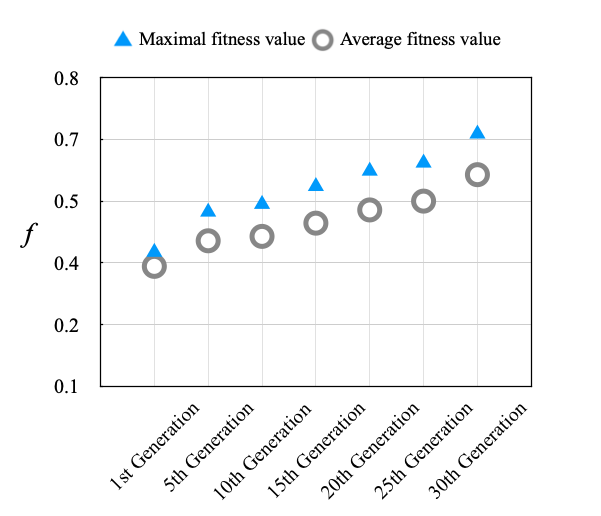
\includegraphics[width=100mm]{results/5/60C_40T.png}
%\caption{\label{fig:5R6040G-fitness} Strategy I - Fitness analysis throughout successive populations ($w_{\rm{CH_4}} = 0.6, w_T = 0.4$, $T_{\rm{in}}$ = 900 K, $u_{\rm{in}}$ = 0.15 m s$^{-1}$, $SC$ = 2.0)}
%\end{figure}

\clearpage


\paragraph{Thermal fitness 20 \%, methane conversion 80 \%} \hspace{0pt} \\
\noindent 



\begin{figure}[h!]
\centering
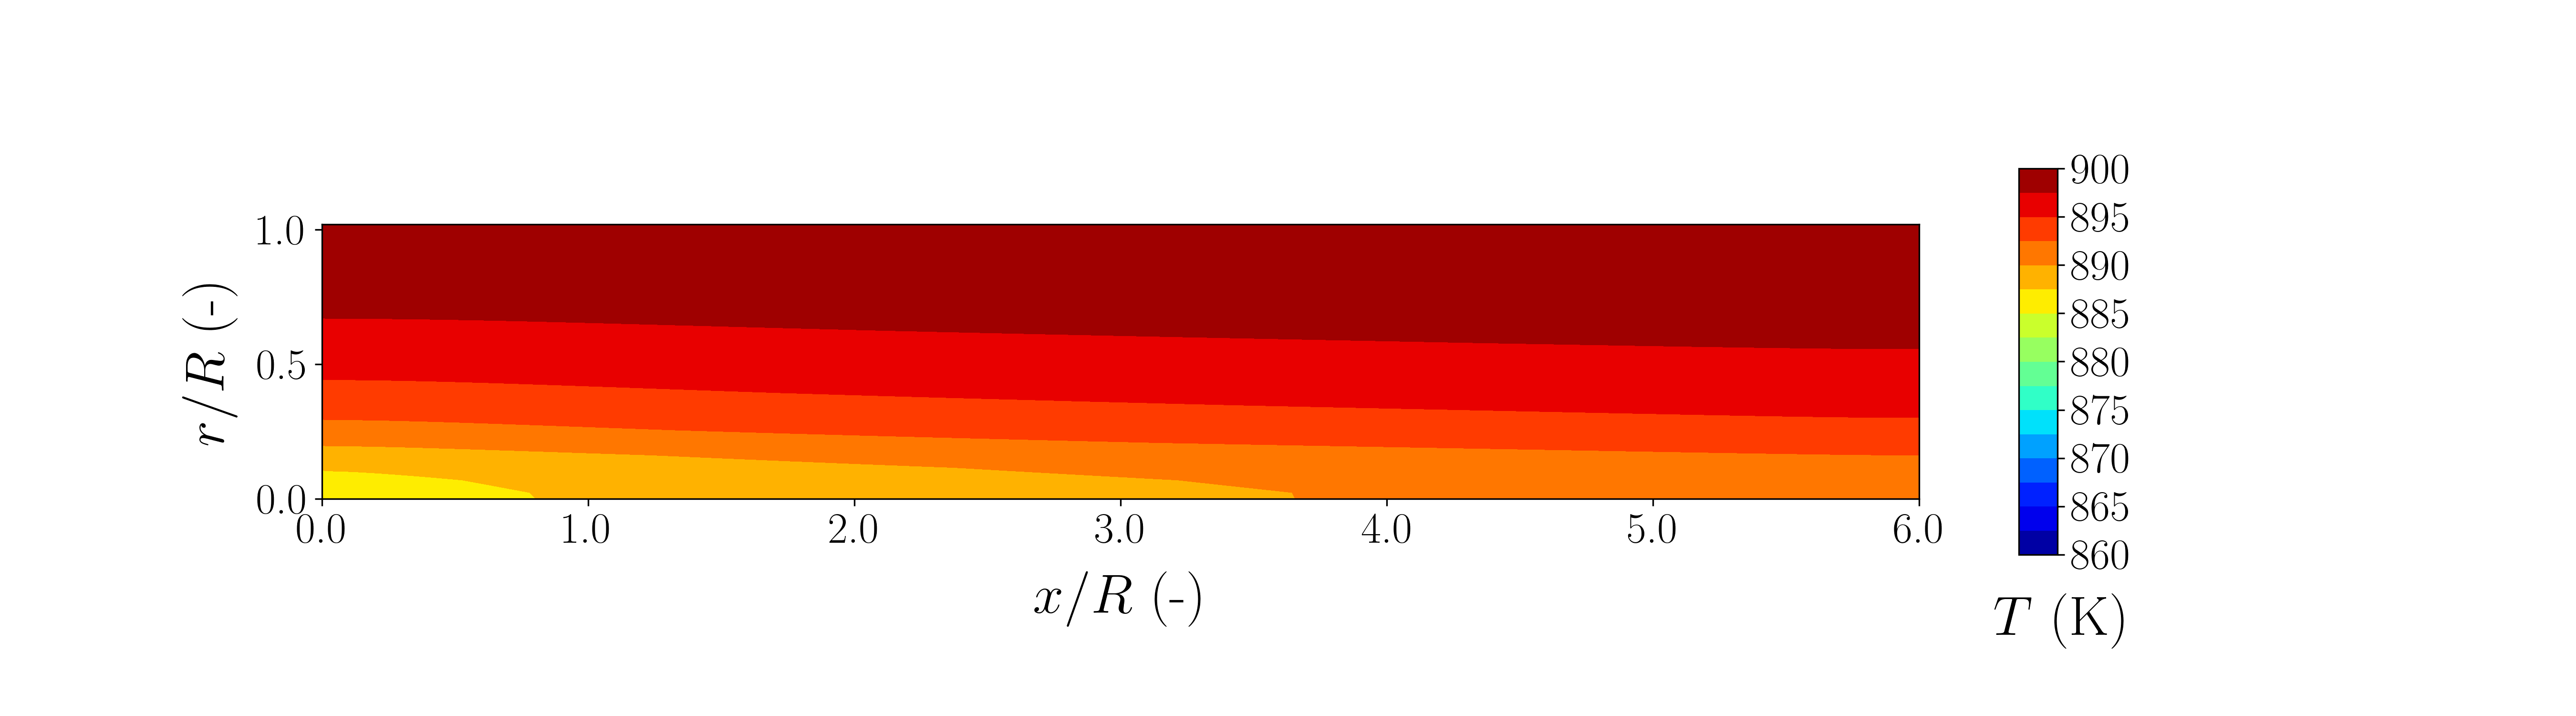
\includegraphics[width=190mm]{results/5/80C_20T/GEN1-TFIELD.png}
\caption{\label{fig:5R8020G1-TField} Strategy I - Temperature field distribution - 1$^{\rm{st}}$ generation ($w_{\rm{CH_4}} = 0.8, w_T = 0.2$, $T_{\rm{in}}$ = 900 K, $u_{\rm{in}}$ = 0.15 m s$^{-1}$, $SC$ = 2.0)}
\end{figure}

\begin{figure}[h!]
\centering
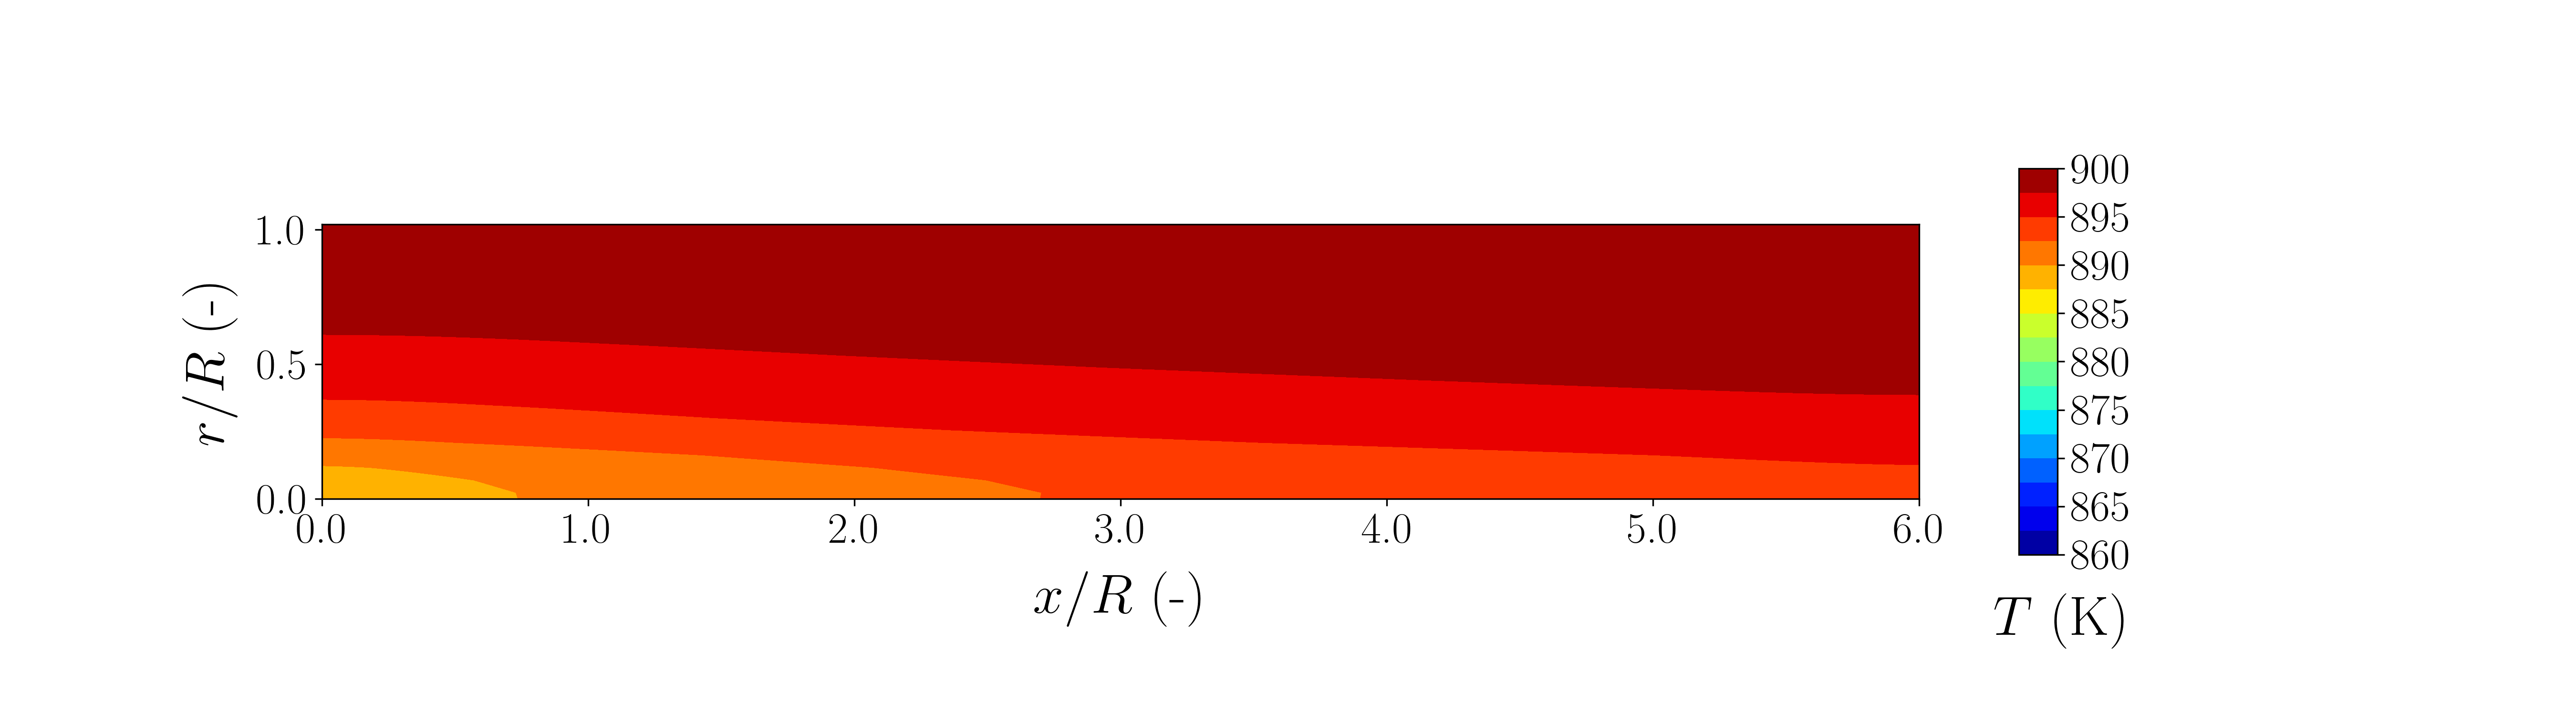
\includegraphics[width=190mm]{results/5/80C_20T/GEN15-TFIELD.png}
\caption{\label{fig:5R8020G15-TField} Strategy I - Temperature field distribution - 15$^{\rm{th}}$ generation ($w_{\rm{CH_4}} = 0.8, w_T = 0.2$, $T_{\rm{in}}$ = 900 K, $u_{\rm{in}}$ = 0.15 m s$^{-1}$, $SC$ = 2.0)}
\end{figure}

\begin{figure}[h!]
\centering
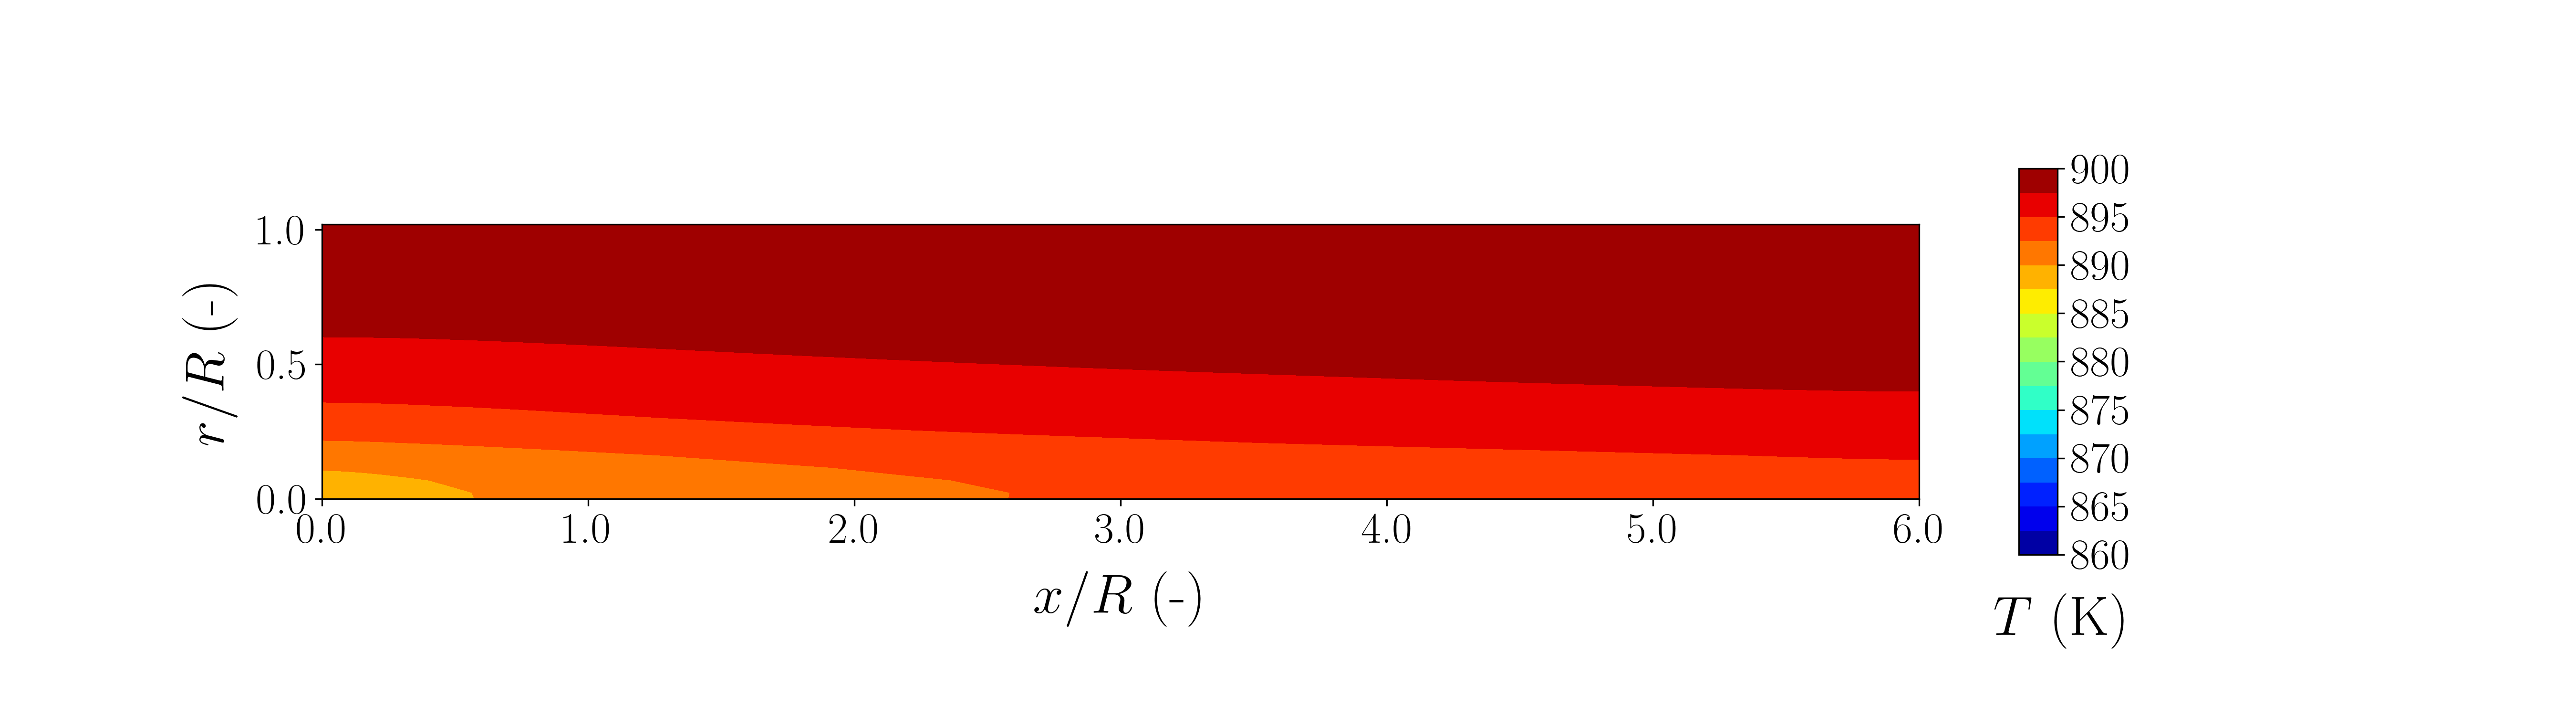
\includegraphics[width=190mm]{results/5/80C_20T/GEN30-TFIELD.png}
\caption{\label{fig:5R8020G30-TField} Strategy I - Temperature field distribution - 30$^{\rm{th}}$ generation ($w_{\rm{CH_4}} = 0.8, w_T = 0.2$, $T_{\rm{in}}$ = 900 K, $u_{\rm{in}}$ = 0.15 m s$^{-1}$, $SC$ = 2.0)}
\end{figure}


\begin{figure}[h!]
\centering
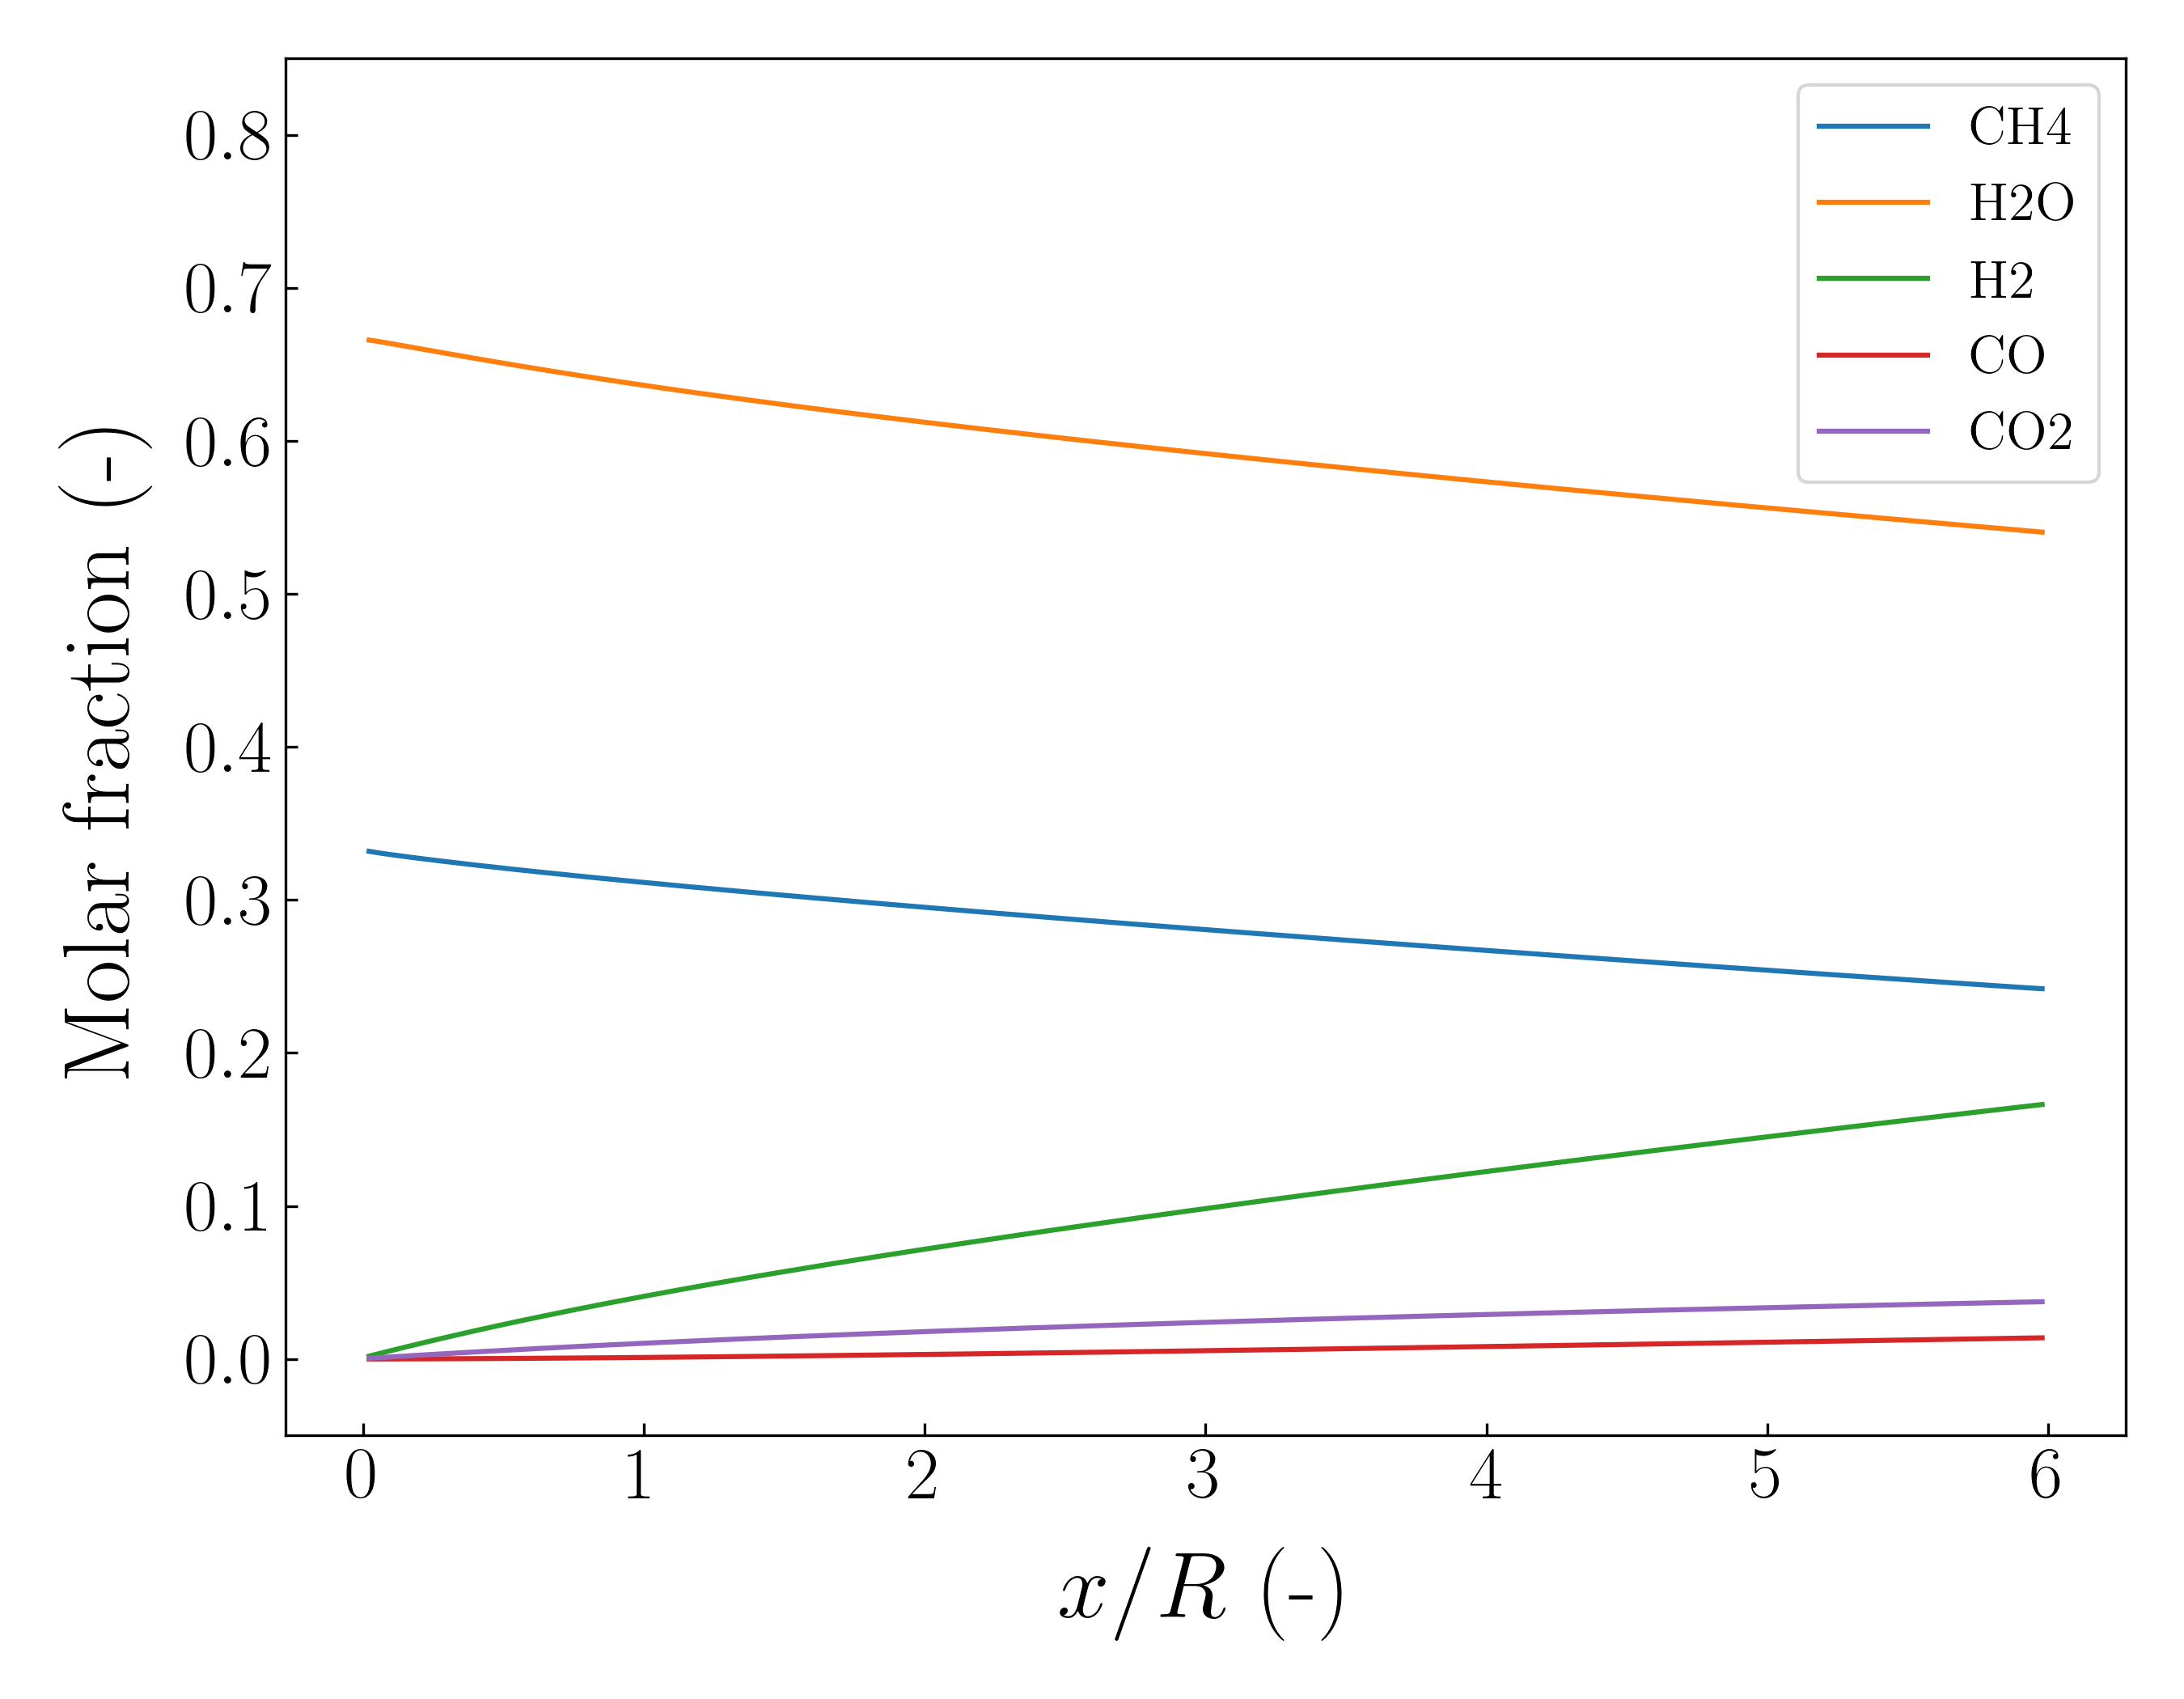
\includegraphics[width=80mm]{results/5/80C_20T/GEN1-AVG.png}
\caption{\label{fig:5R8020G1-avg} Strategy I - Radius-averaged molar fractions - 1$^{\rm{st}}$ generation ($w_{\rm{CH_4}} = 0.8, w_T = 0.2$, $T_{\rm{in}}$ = 900 K, $u_{\rm{in}}$ = 0.15 m s$^{-1}$, $SC$ = 2.0)}
\end{figure}

\begin{figure}[h!]
\centering
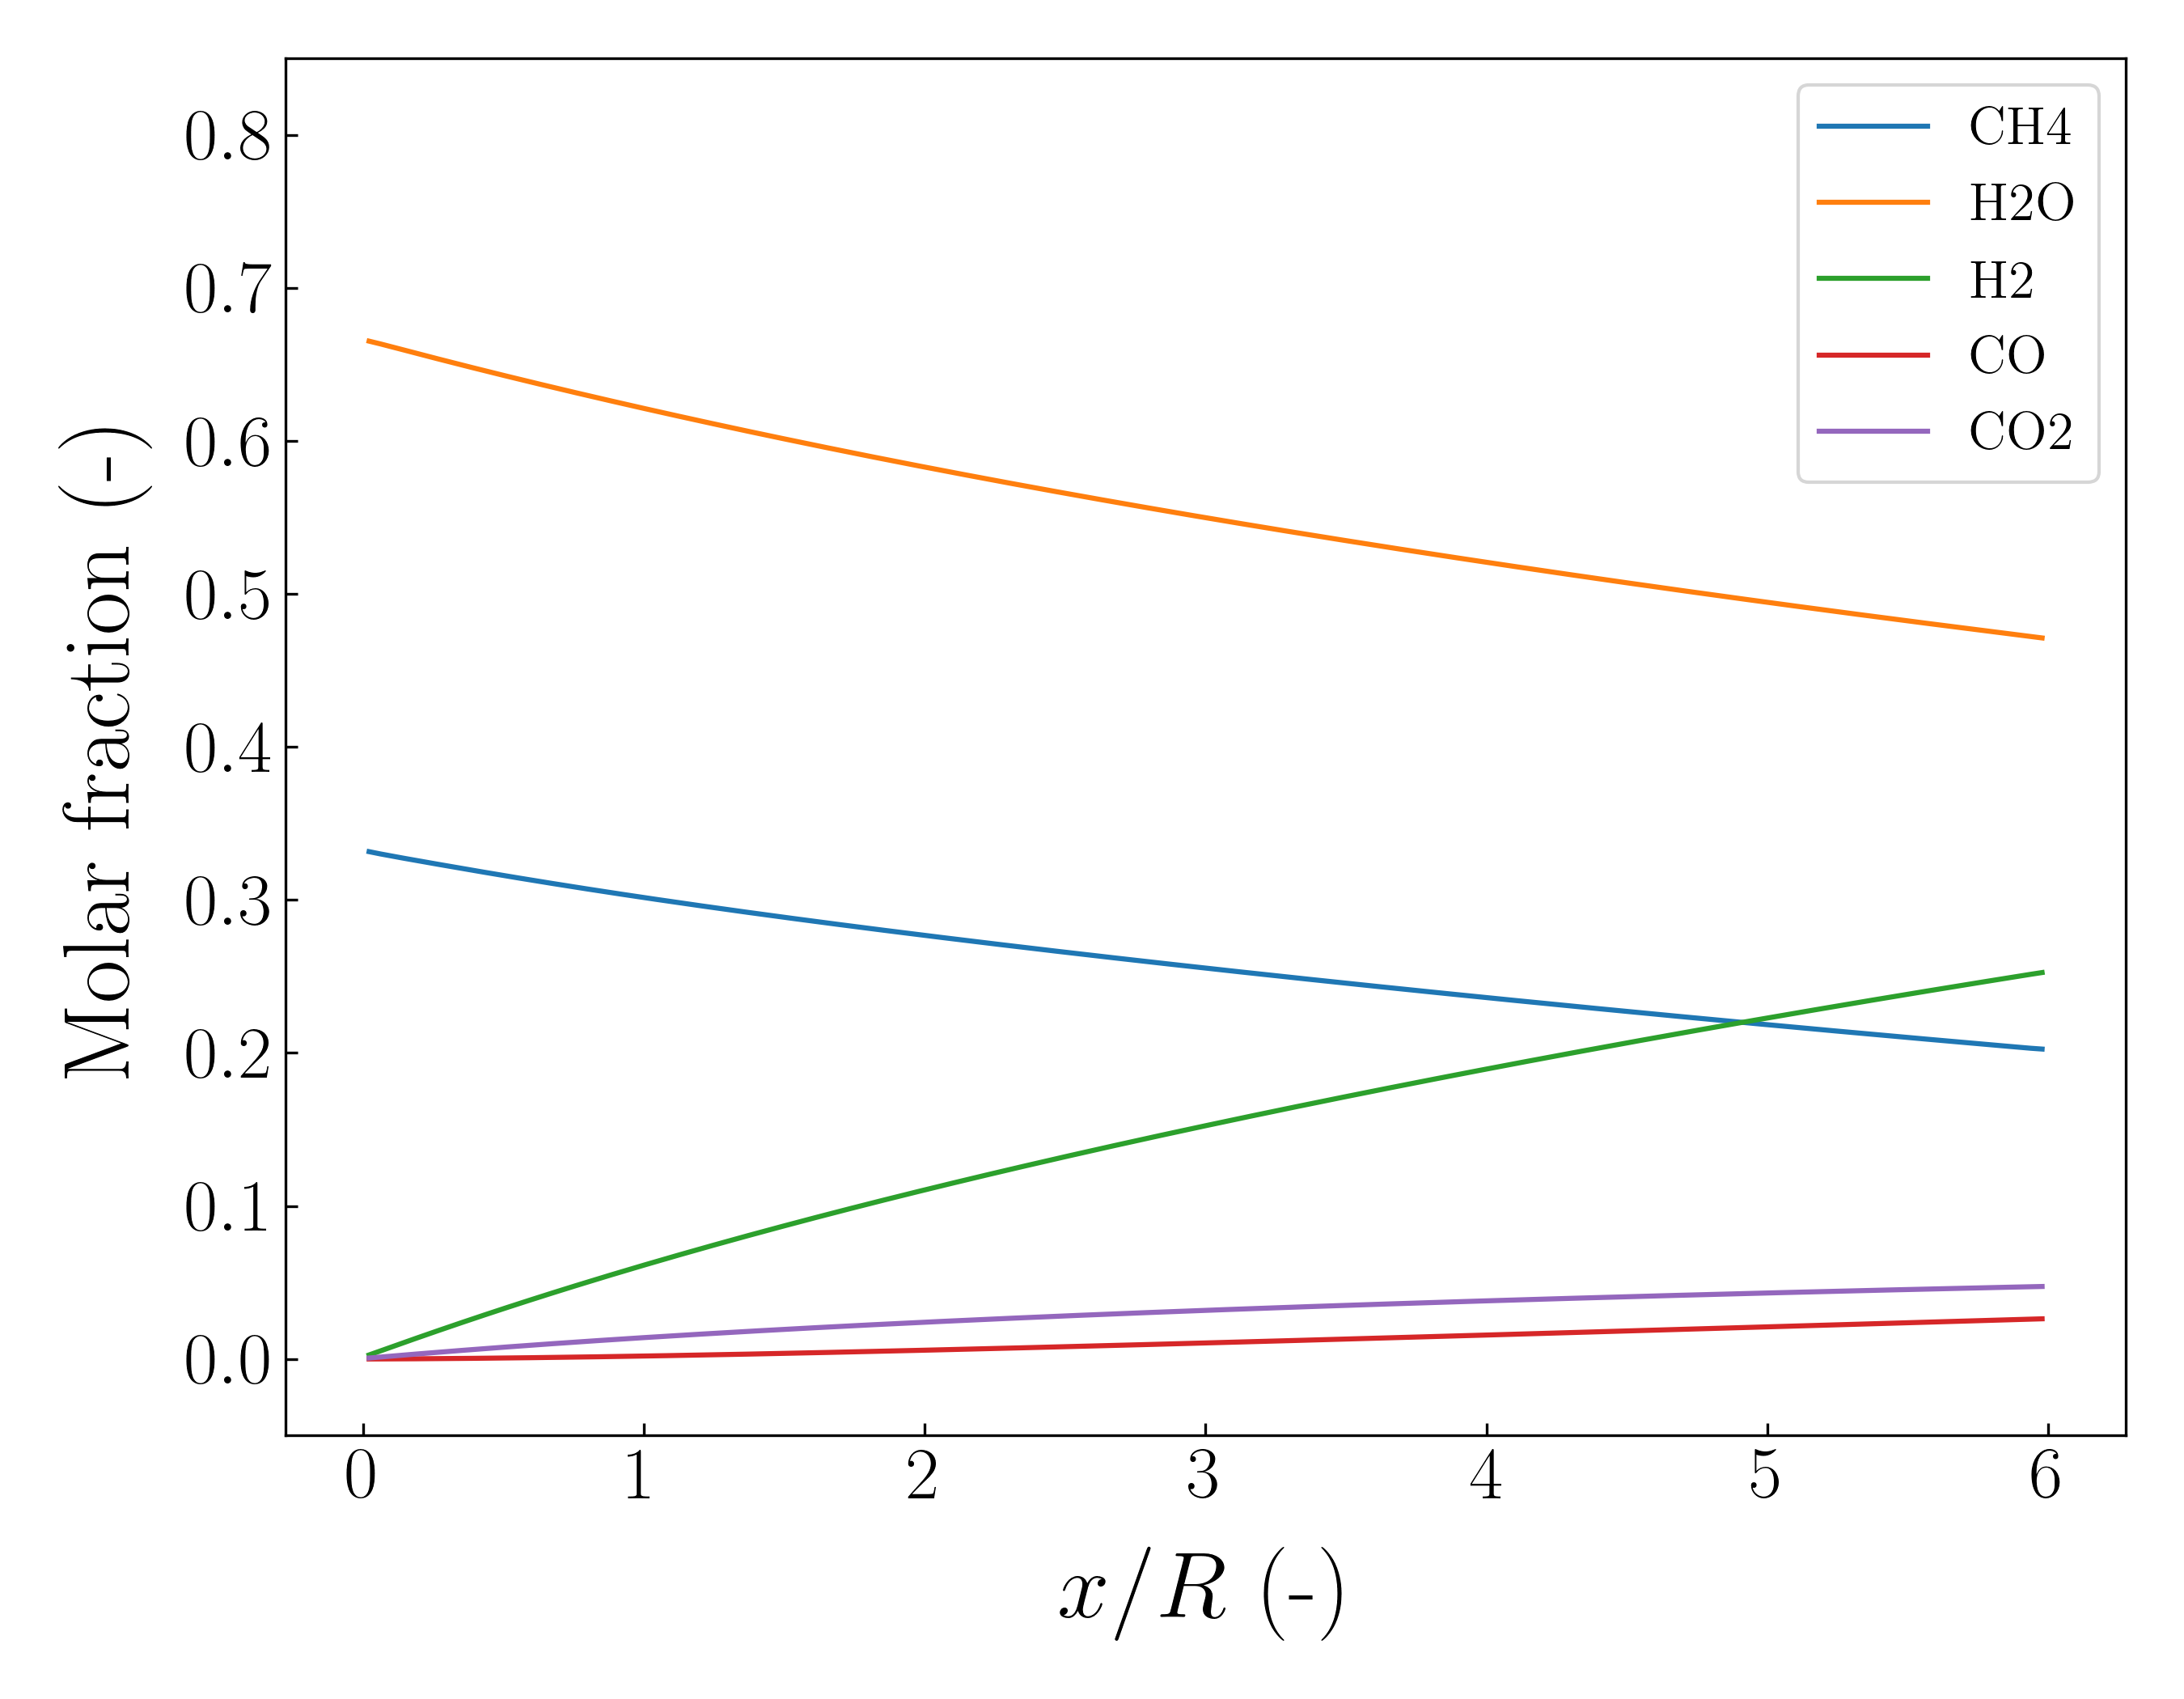
\includegraphics[width=80mm]{results/5/80C_20T/GEN15-AVG.png}
\caption{\label{fig:5R8020G15-avg} Strategy I - Radius-averaged molar fractions - 15$^{\rm{th}}$ generation ($w_{\rm{CH_4}} = 0.8, w_T = 0.2$, $T_{\rm{in}}$ = 900 K, $u_{\rm{in}}$ = 0.15 m s$^{-1}$, $SC$ = 2.0)}
\end{figure}

\begin{figure}[h!]
\centering
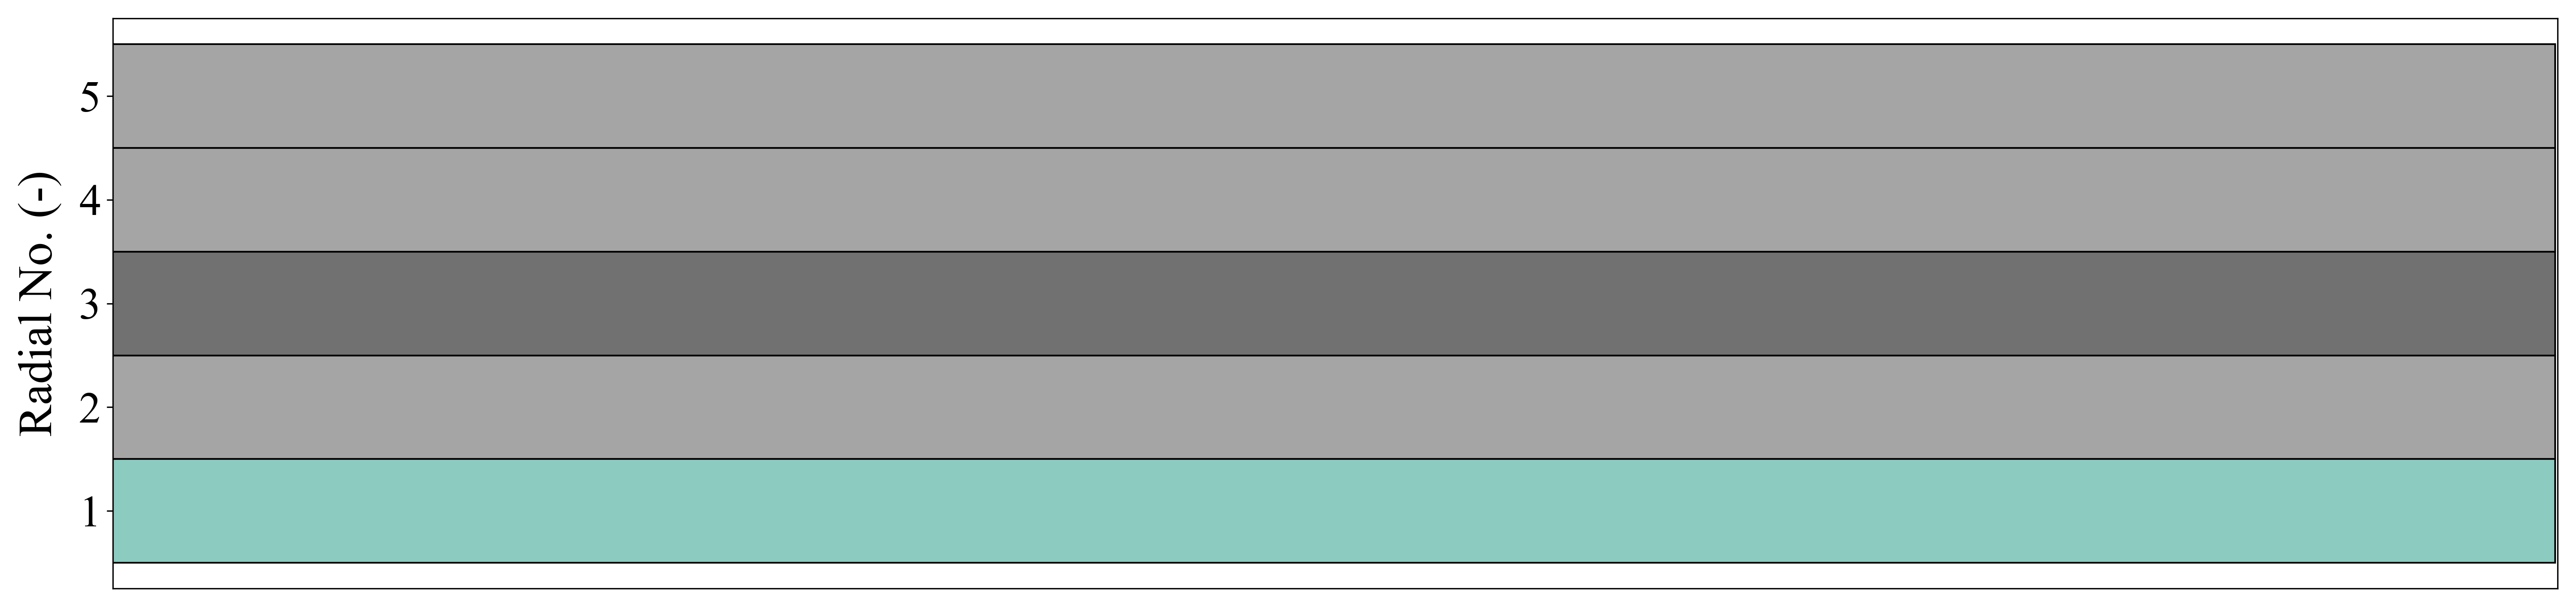
\includegraphics[width=120mm]{results/segments/5seg/80C20T/seg.png}
\caption{\label{fig:30L6040G1-TField} Strategy I - Segments distribution for 30$^{\rm{th}}$ generation ($w_{\rm{CH_4}} = 0.8, w_T = 0.2$, $T_{\rm{in}}$ = 900 K, $u_{\rm{in}}$ = 0.15 m s$^{-1}$, $SC$ = 2.0)}
\end{figure}

\begin{figure}[h!]
\centering
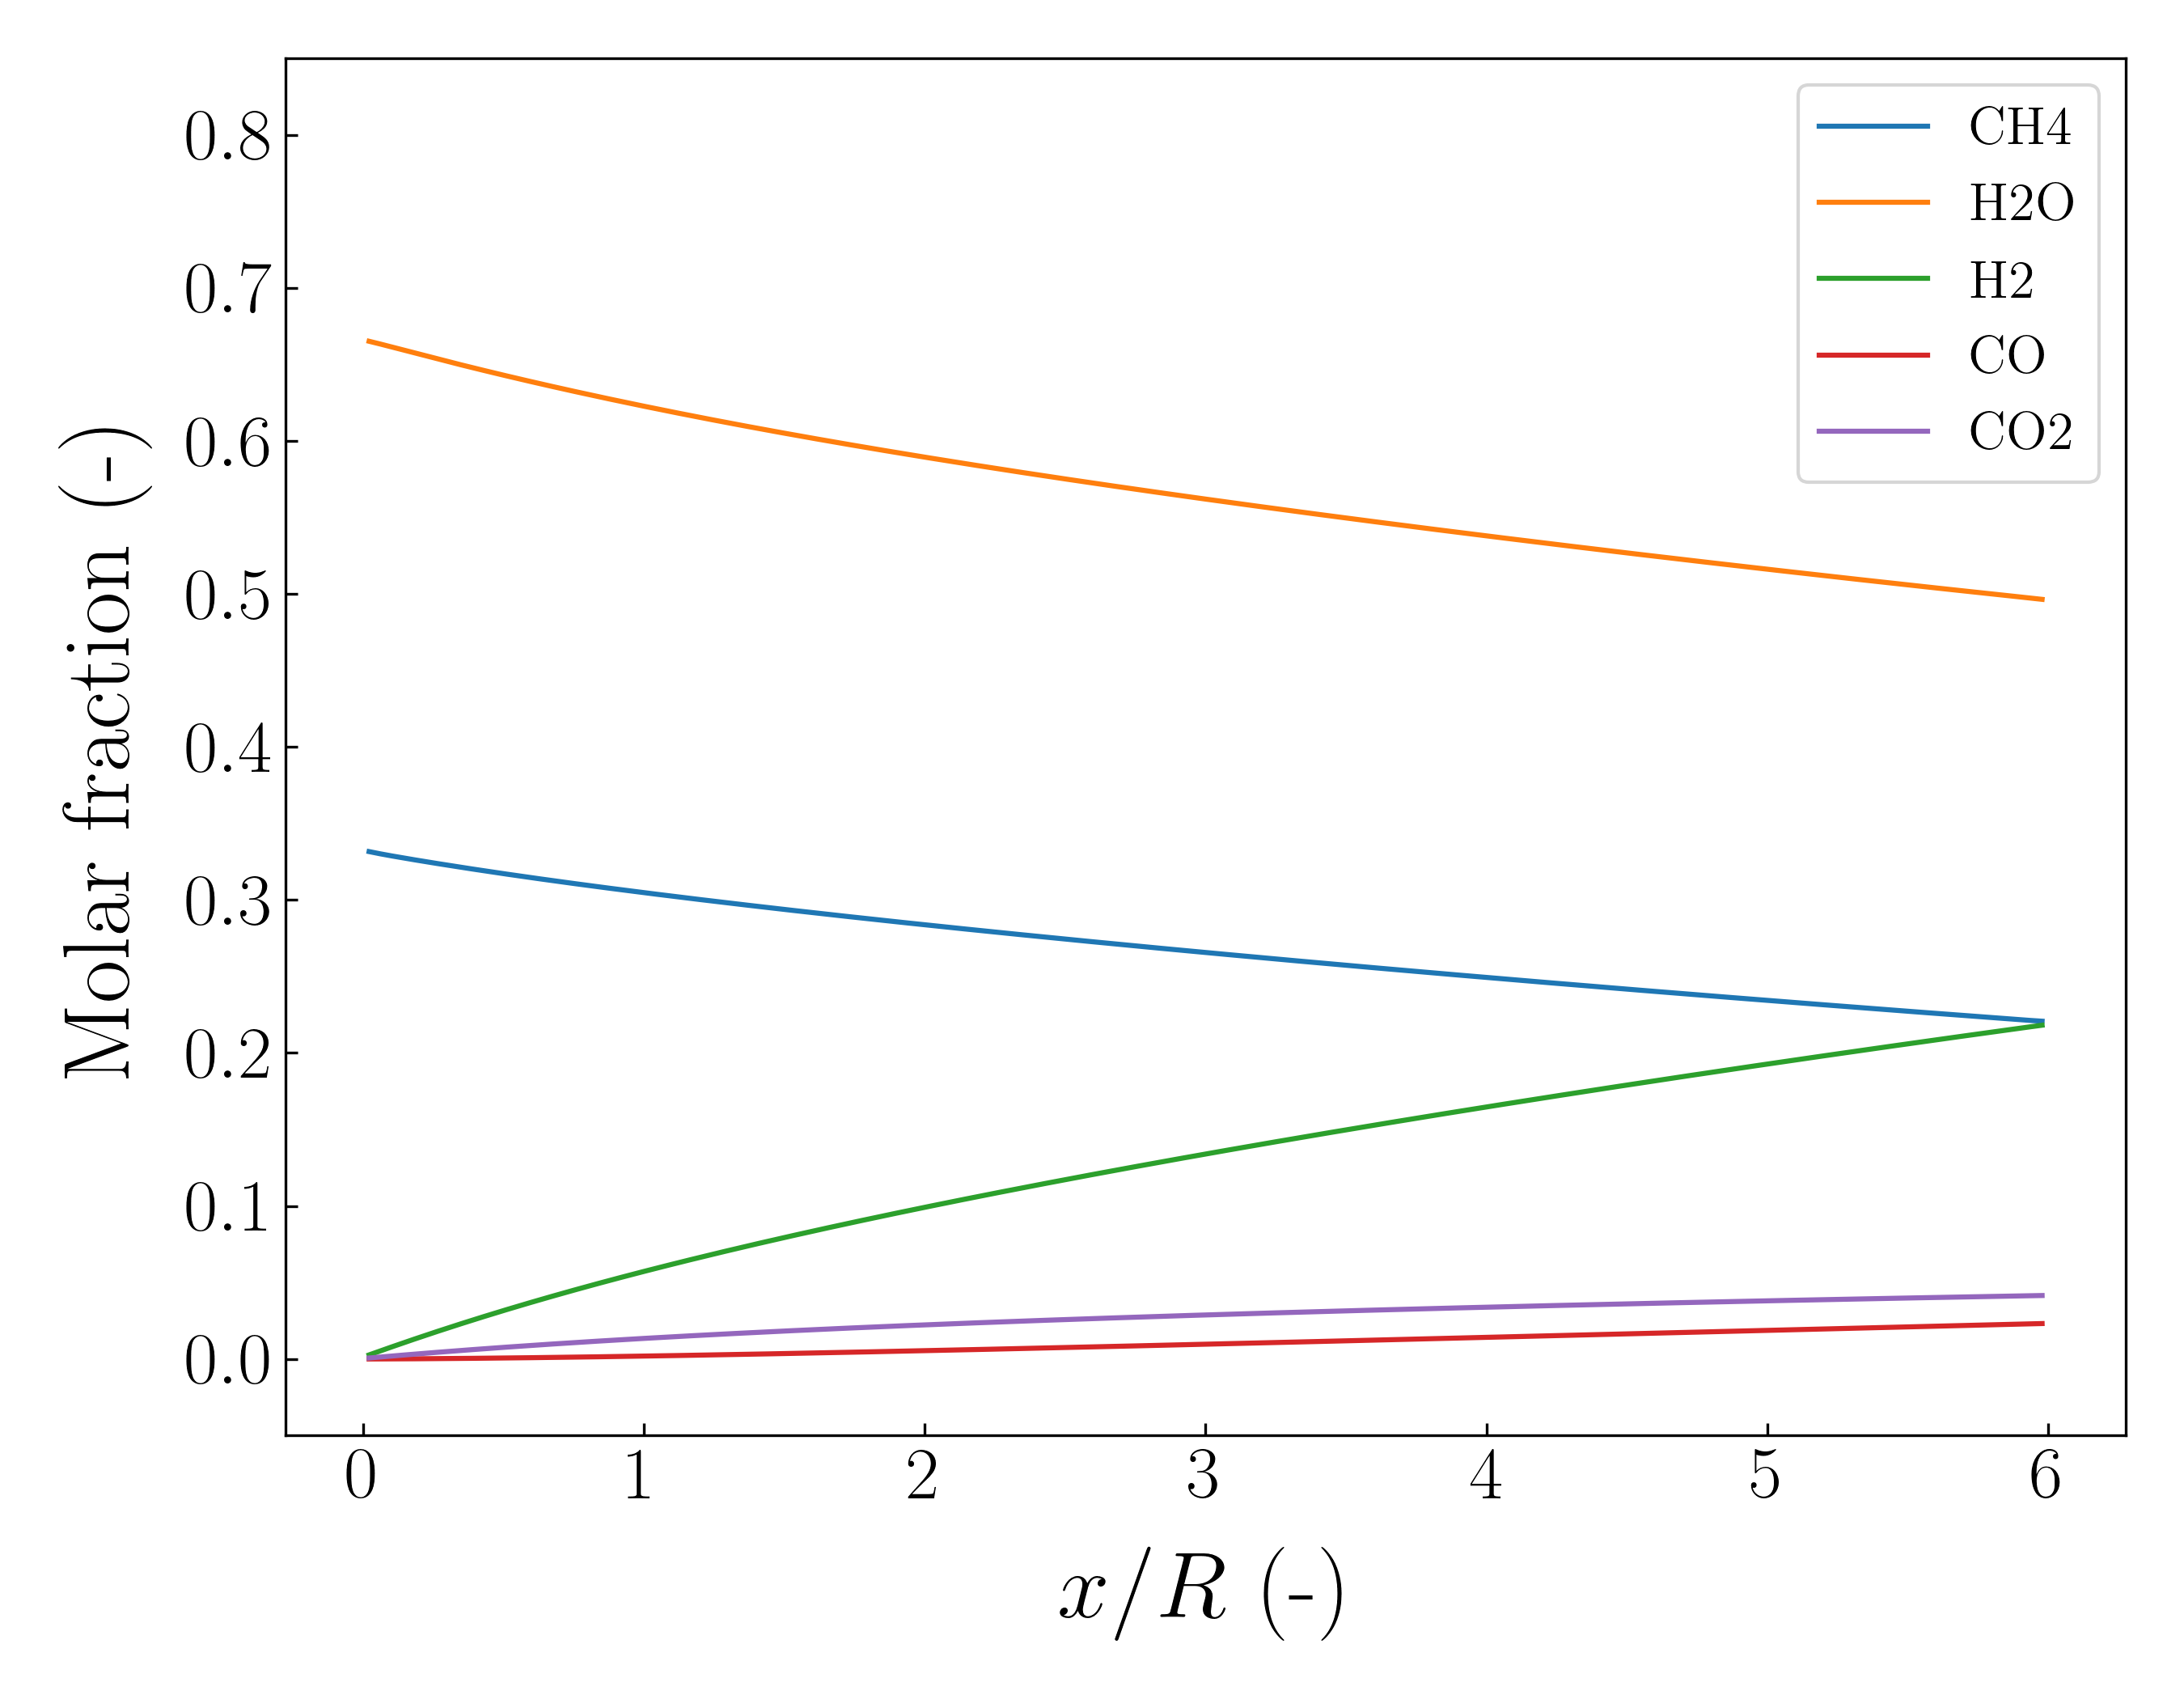
\includegraphics[width=80mm]{results/5/80C_20T/GEN30-AVG.png}
\caption{\label{fig:5R8020G30-avg} Strategy I - Radius-averaged molar fractions -  30$^{\rm{th}}$ generation ($w_{\rm{CH_4}} = 0.8, w_T = 0.2$, $T_{\rm{in}}$ = 900 K, $u_{\rm{in}}$ = 0.15 m s$^{-1}$, $SC$ = 2.0)}
\end{figure}


The development of the fitness values among successive populations for strategy I is presented in Fig. \ref{fig:5R8020G-fitness}. 

%\begin{figure}
%\centering
%\includegraphics[width=100mm]{results/5/80C_20T.png}
%\caption{\label{fig:5R8020G-fitness} Strategy I - Fitness analysis throughout successive populations ($w_{\rm{CH_4}} = 0.8, w_T = 0.2$, $T_{\rm{in}}$ = 900 K, $u_{\rm{in}}$ = 0.15 m s$^{-1}$, $SC$ = 2.0)}
%\end{figure}

To allow a straightforward comparison between the catalyst inserts division strategies, hydrogen productivity $\zeta$ is calculated for the optimal cases found by each algorithm. The hydrogen productivity is summarized in Table \ref{tab:5RH2prod}. 

\begin{center}
\begin{table}
\centering
\caption{Hydrogen productivity for the catalytic insert division strategy I}
\label{tab:5RH2prod}
\begin{tabular}{l|c|c|c}
\hline\noalign{\smallskip}
 $w_{\rm{CH_4}}$ / $ w_T $ & $\rm{H_{2_{out}}}$ & $\iota$ & $\zeta$ \\
\noalign{\smallskip}\hline\noalign{\smallskip}
REF         & 0.581     & 1.00  &  0.581\\
0.2 / 0.8   & 0.255     & 0.20  & 1.278 \\
0.4 / 0.6   & 0.268     & 0.19  & 1.398 \\
0.5 / 0.5   & 0.231     & 0.20  & 1.157 \\
0.6 / 0.4   & 0.407     & 0.45  & 0.900 \\
0.8 / 0.2   & 0.218     & 0.20  & 1.090 \\
\noalign{\smallskip}\hline
\end{tabular}
\end{table}
\end{center}


\clearpage


\subsection{Insert division strategy II}
\label{subsec:5RE}

\begin{figure}[h!]
\centering
\includegraphics[width=120mm]{5segEqSurf.png}
\caption{\label{fig:5segEqSurf}Catalytic insert division strategy II}
\end{figure}


\paragraph{Thermal fitness 80 \%, methane conversion 20 \%} \hspace{0pt} \\
\noindent 


\begin{figure}[h!]
\centering
\includegraphics[width=190mm]{results/5Eq/20C_80T/GEN1-TFIELD.png}
\caption{\label{fig:5RES2080G1-TField} Strategy II - Temperature field distribution - 1$^{\rm{st}}$ generation ($w_{\rm{CH_4}} = 0.2, w_T = 0.8$, $T_{\rm{in}}$ = 900 K, $u_{\rm{in}}$ = 0.15 m s$^{-1}$, $SC$ = 2.0)}
\end{figure}

\begin{figure}[h!]
\centering
\includegraphics[width=190mm]{results/5Eq/20C_80T/GEN15-TFIELD.png}
\caption{\label{fig:5RES2080G15-TField} Strategy II - Temperature field distribution - 15$^{\rm{th}}$ generation ($w_{\rm{CH_4}} = 0.2, w_T = 0.8$, $T_{\rm{in}}$ = 900 K, $u_{\rm{in}}$ = 0.15 m s$^{-1}$, $SC$ = 2.0)}
\end{figure}

\begin{figure}[h!]
\centering
\includegraphics[width=190mm]{results/5Eq/20C_80T/GEN30-TFIELD.png}
\caption{\label{fig:5RES2080G30-TField} Strategy II - Temperature field distribution - 30$^{\rm{th}}$ generation ($w_{\rm{CH_4}} = 0.2, w_T = 0.8$, $T_{\rm{in}}$ = 900 K, $u_{\rm{in}}$ = 0.15 m s$^{-1}$, $SC$ = 2.0)}
\end{figure}


\begin{figure}[h!]
\centering
\includegraphics[width=80mm]{results/5Eq/20C_80T/GEN1-AVG.png}
\caption{\label{fig:5RES2080G1-avg} Strategy II - Radius-averaged molar fractions - 1$^{\rm{st}}$ generation ($w_{\rm{CH_4}} = 0.2, w_T = 0.8$, $T_{\rm{in}}$ = 900 K, $u_{\rm{in}}$ = 0.15 m s$^{-1}$, $SC$ = 2.0)}
\end{figure}

\begin{figure}[h!]
\centering
\includegraphics[width=80mm]{results/5Eq/20C_80T/GEN15-AVG.png}
\caption{\label{fig:5RES2080G15-avg} Strategy II - Radius-averaged molar fractions - 15$^{\rm{th}}$ generation ($w_{\rm{CH_4}} = 0.2, w_T = 0.8$, $T_{\rm{in}}$ = 900 K, $u_{\rm{in}}$ = 0.15 m s$^{-1}$, $SC$ = 2.0)}
\end{figure}

\begin{figure}[h!]
\centering
\includegraphics[width=80mm]{results/5Eq/20C_80T/GEN30-AVG.png}
\caption{\label{fig:5RES2080G30-avg} Strategy II - Radius-averaged molar fractions -  30$^{\rm{th}}$ generation ($w_{\rm{CH_4}} = 0.2, w_T = 0.8$, $T_{\rm{in}}$ = 900 K, $u_{\rm{in}}$ = 0.15 m s$^{-1}$, $SC$ = 2.0)}
\end{figure}

\begin{figure}[h!]
\centering
\includegraphics[width=120mm]{results/segments/5segEq/20C80T/seg.png}
\caption{\label{fig:30L6040G1-TField} Strategy II - Segments distribution for 30$^{\rm{th}}$ generation ($w_{\rm{CH_4}} = 0.2, w_T = 0.8$, $T_{\rm{in}}$ = 900 K, $u_{\rm{in}}$ = 0.15 m s$^{-1}$, $SC$ = 2.0)}
\end{figure}

%\begin{figure}[h!]
%\centering
%\includegraphics[width=100mm]{results/5Eq/20C_80T.png}
%\caption{\label{fig:5RES2080G-fitness} Strategy II - Fitness analysis throughout successive populations ($w_{\rm{CH_4}} = 0.2, w_T = 0.8$, $T_{\rm{in}}$ = 900 K, $u_{\rm{in}}$ = 0.15 m s$^{-1}$, $SC$ = 2.0)}
%\end{figure}



\clearpage



\paragraph{Thermal fitness 60 \%, methane conversion 40 \%} \hspace{0pt} \\
\noindent 


\begin{figure}[h!]
\centering
\includegraphics[width=190mm]{results/5Eq/40C_60T/GEN1-TFIELD.png}
\caption{\label{fig:5RES4060G1-TField} Strategy II - Temperature field distribution - 1$^{\rm{st}}$ generation ($w_{\rm{CH_4}} = 0.4, w_T = 0.6$, $T_{\rm{in}}$ = 900 K, $u_{\rm{in}}$ = 0.15 m s$^{-1}$, $SC$ = 2.0)}
\end{figure}

\begin{figure}[h!]
\centering
\includegraphics[width=190mm]{results/5Eq/40C_60T/GEN15-TFIELD.png}
\caption{\label{fig:5RES4060G15-TField} Strategy II - Temperature field distribution - 15$^{\rm{th}}$ generation ($w_{\rm{CH_4}} = 0.4, w_T = 0.6$, $T_{\rm{in}}$ = 900 K, $u_{\rm{in}}$ = 0.15 m s$^{-1}$, $SC$ = 2.0)}
\end{figure}

\begin{figure}[h!]
\centering
\includegraphics[width=190mm]{results/5Eq/40C_60T/GEN30-TFIELD.png}
\caption{\label{fig:5RES4060G30-TField} Strategy II - Temperature field distribution - 30$^{\rm{th}}$ generation ($w_{\rm{CH_4}} = 0.4, w_T = 0.6$, $T_{\rm{in}}$ = 900 K, $u_{\rm{in}}$ = 0.15 m s$^{-1}$, $SC$ = 2.0)}
\end{figure}


\begin{figure}[h!]
\centering
\includegraphics[width=80mm]{results/5Eq/40C_60T/GEN1-AVG.png}
\caption{\label{fig:5RES4060G1-avg} Strategy II - Radius-averaged molar fractions - 1$^{\rm{st}}$ generation ($w_{\rm{CH_4}} = 0.4, w_T = 0.6$, $T_{\rm{in}}$ = 900 K, $u_{\rm{in}}$ = 0.15 m s$^{-1}$, $SC$ = 2.0)}
\end{figure}

\begin{figure}[h!]
\centering
\includegraphics[width=80mm]{results/5Eq/40C_60T/GEN15-AVG.png}
\caption{\label{fig:5RES4060G15-avg} Strategy II - Radius-averaged molar fractions - 15$^{\rm{th}}$ generation ($w_{\rm{CH_4}} = 0.4, w_T = 0.6$, $T_{\rm{in}}$ = 900 K, $u_{\rm{in}}$ = 0.15 m s$^{-1}$, $SC$ = 2.0)}
\end{figure}

\begin{figure}[h!]
\centering
\includegraphics[width=80mm]{results/5Eq/40C_60T/GEN30-AVG.png}
\caption{\label{fig:5RES4060G30-avg} Strategy II - Radius-averaged molar fractions -  30$^{\rm{th}}$ generation ($w_{\rm{CH_4}} = 0.4, w_T = 0.6$, $T_{\rm{in}}$ = 900 K, $u_{\rm{in}}$ = 0.15 m s$^{-1}$, $SC$ = 2.0)}
\end{figure}

\begin{figure}[h!]
\centering
\includegraphics[width=120mm]{results/segments/5segEq/40C60T/seg.png}
\caption{\label{fig:30L6040G1-TField} Strategy II - Segments distribution for 30$^{\rm{th}}$ generation ($w_{\rm{CH_4}} = 0.4, w_T = 0.6$, $T_{\rm{in}}$ = 900 K, $u_{\rm{in}}$ = 0.15 m s$^{-1}$, $SC$ = 2.0)}
\end{figure}

%\begin{figure}[h!]
%\centering
%\includegraphics[width=100mm]{results/5Eq/40C_60T.png}
%\caption{\label{fig:5RES4060G-fitness} Strategy II - Fitness analysis throughout successive populations ($w_{\rm{CH_4}} = 0.4, w_T = 0.6$, $T_{\rm{in}}$ = 900 K, $u_{\rm{in}}$ = 0.15 m s$^{-1}$, $SC$ = 2.0)}
%\end{figure}


\clearpage





\paragraph{Thermal fitness 50 \%, methane conversion 50 \%} \hspace{0pt} \\
\noindent 


\begin{figure}[h!]
\centering
\includegraphics[width=190mm]{results/5Eq/50C_50T/GEN1-TFIELD.png}
\caption{\label{fig:5RES5050G1-TField} Strategy II - Temperature field distribution - 1$^{\rm{st}}$ generation ($w_{\rm{CH_4}} = 0.5, w_T = 0.5$, $T_{\rm{in}}$ = 900 K, $u_{\rm{in}}$ = 0.15 m s$^{-1}$, $SC$ = 2.0)}
\end{figure}

\begin{figure}[h!]
\centering
\includegraphics[width=190mm]{results/5Eq/50C_50T/GEN15-TFIELD.png}
\caption{\label{fig:5RES5050G15-TField} Strategy II - Temperature field distribution - 15$^{\rm{th}}$ generation ($w_{\rm{CH_4}} = 0.5, w_T = 0.5$, $T_{\rm{in}}$ = 900 K, $u_{\rm{in}}$ = 0.15 m s$^{-1}$, $SC$ = 2.0)}
\end{figure}

\begin{figure}[h!]
\centering
\includegraphics[width=190mm]{results/5Eq/50C_50T/GEN30-TFIELD.png}
\caption{\label{fig:5RES5050G30-TField} Strategy II - Temperature field distribution - 30$^{\rm{th}}$ generation ($w_{\rm{CH_4}} = 0.5, w_T = 0.5$, $T_{\rm{in}}$ = 900 K, $u_{\rm{in}}$ = 0.15 m s$^{-1}$, $SC$ = 2.0)}
\end{figure}


\begin{figure}[h!]
\centering
\includegraphics[width=80mm]{results/5Eq/50C_50T/GEN1-AVG.png}
\caption{\label{fig:5RES5050G1-avg} Strategy II - Radius-averaged molar fractions - 1$^{\rm{st}}$ generation ($w_{\rm{CH_4}} = 0.5, w_T = 0.5$, $T_{\rm{in}}$ = 900 K, $u_{\rm{in}}$ = 0.15 m s$^{-1}$, $SC$ = 2.0)}
\end{figure}

\begin{figure}[h!]
\centering
\includegraphics[width=80mm]{results/5Eq/50C_50T/GEN15-AVG.png}
\caption{\label{fig:5RES5050G15-avg} Strategy II - Radius-averaged molar fractions - 15$^{\rm{th}}$ generation ($w_{\rm{CH_4}} = 0.5, w_T = 0.5$, $T_{\rm{in}}$ = 900 K, $u_{\rm{in}}$ = 0.15 m s$^{-1}$, $SC$ = 2.0)}
\end{figure}

\begin{figure}[h!]
\centering
\includegraphics[width=80mm]{results/5Eq/50C_50T/GEN30-AVG.png}
\caption{\label{fig:5RES5050G30-avg} Strategy II - Radius-averaged molar fractions -  30$^{\rm{th}}$ generation ($w_{\rm{CH_4}} = 0.5, w_T = 0.5$, $T_{\rm{in}}$ = 900 K, $u_{\rm{in}}$ = 0.15 m s$^{-1}$, $SC$ = 2.0)}
\end{figure}

\begin{figure}[h!]
\centering
\includegraphics[width=120mm]{results/segments/5segEq/50C50T/seg.png}
\caption{\label{fig:30L6040G1-TField} Strategy II - Segments distribution for 30$^{\rm{th}}$ generation ($w_{\rm{CH_4}} = 0.5, w_T = 0.5$, $T_{\rm{in}}$ = 900 K, $u_{\rm{in}}$ = 0.15 m s$^{-1}$, $SC$ = 2.0)}
\end{figure}


%\begin{figure}[h!]
%\centering
%\includegraphics[width=100mm]{results/5Eq/50C_50T.png}
%\caption{\label{fig:5RES5050G-fitness} Strategy II - Fitness analysis throughout successive populations ($w_{\rm{CH_4}} = 0.5, w_T = 0.5$, $T_{\rm{in}}$ = 900 K, $u_{\rm{in}}$ = 0.15 m s$^{-1}$, $SC$ = 2.0)}
%\end{figure}


\clearpage



\paragraph{Thermal fitness 40 \%, methane conversion 60 \%} \hspace{0pt} \\
\noindent 


\begin{figure}[h!]
\centering
\includegraphics[width=190mm]{results/5Eq/60C_40T/GEN1-TFIELD.png}
\caption{\label{fig:5RES6040G1-TField} Strategy II - Temperature field distribution - 1$^{\rm{st}}$ generation ($w_{\rm{CH_4}} = 0.6, w_T = 0.4$, $T_{\rm{in}}$ = 900 K, $u_{\rm{in}}$ = 0.15 m s$^{-1}$, $SC$ = 2.0)}
\end{figure}

\begin{figure}[h!]
\centering
\includegraphics[width=190mm]{results/5Eq/60C_40T/GEN15-TFIELD.png}
\caption{\label{fig:5RES6040G15-TField} Strategy II - Temperature field distribution - 15$^{\rm{th}}$ generation ($w_{\rm{CH_4}} = 0.6, w_T = 0.4$, $T_{\rm{in}}$ = 900 K, $u_{\rm{in}}$ = 0.15 m s$^{-1}$, $SC$ = 2.0)}
\end{figure}

\begin{figure}[h!]
\centering
\includegraphics[width=190mm]{results/5Eq/60C_40T/GEN30-TFIELD.png}
\caption{\label{fig:5RES6040G30-TField} Strategy II - Temperature field distribution - 30$^{\rm{th}}$ generation ($w_{\rm{CH_4}} = 0.6, w_T = 0.4$, $T_{\rm{in}}$ = 900 K, $u_{\rm{in}}$ = 0.15 m s$^{-1}$, $SC$ = 2.0)}
\end{figure}


\begin{figure}[h!]
\centering
\includegraphics[width=80mm]{results/5Eq/60C_40T/GEN1-AVG.png}
\caption{\label{fig:5RES6040G1-avg} Strategy II - Radius-averaged molar fractions - 1$^{\rm{st}}$ generation ($w_{\rm{CH_4}} = 0.6, w_T = 0.4$, $T_{\rm{in}}$ = 900 K, $u_{\rm{in}}$ = 0.15 m s$^{-1}$, $SC$ = 2.0)}
\end{figure}

\begin{figure}[h!]
\centering
\includegraphics[width=80mm]{results/5Eq/60C_40T/GEN15-AVG.png}
\caption{\label{fig:5RES6040G15-avg} Strategy II - Radius-averaged molar fractions - 15$^{\rm{th}}$ generation ($w_{\rm{CH_4}} = 0.6, w_T = 0.4$, $T_{\rm{in}}$ = 900 K, $u_{\rm{in}}$ = 0.15 m s$^{-1}$, $SC$ = 2.0)}
\end{figure}

\begin{figure}[h!]
\centering
\includegraphics[width=80mm]{results/5Eq/60C_40T/GEN30-AVG.png}
\caption{\label{fig:5RES6040G30-avg} Strategy II - Radius-averaged molar fractions -  30$^{\rm{th}}$ generation ($w_{\rm{CH_4}} = 0.6, w_T = 0.4$, $T_{\rm{in}}$ = 900 K, $u_{\rm{in}}$ = 0.15 m s$^{-1}$, $SC$ = 2.0)}
\end{figure}

\begin{figure}[h!]
\centering
\includegraphics[width=120mm]{results/segments/5segEq/60C40T/seg.png}
\caption{\label{fig:30L6040G1-TField} Strategy II - Segments distribution for 30$^{\rm{th}}$ generation ($w_{\rm{CH_4}} = 0.6, w_T = 0.4$, $T_{\rm{in}}$ = 900 K, $u_{\rm{in}}$ = 0.15 m s$^{-1}$, $SC$ = 2.0)}
\end{figure}

%\begin{figure}[h!]
%\centering
%\includegraphics[width=100mm]{results/5Eq/60C_40T.png}
%\caption{\label{fig:5RES6040G-fitness} Strategy II - Fitness analysis throughout successive populations ($w_{\rm{CH_4}} = 0.6, w_T = 0.4$, $T_{\rm{in}}$ = 900 K, $u_{\rm{in}}$ = 0.15 m s$^{-1}$, $SC$ = 2.0)}
%\end{figure}

\clearpage


\paragraph{Thermal fitness 20 \%, methane conversion 80 \%} \hspace{0pt} \\
\noindent 



\begin{figure}[h!]
\centering
\includegraphics[width=190mm]{results/5Eq/80C_20T/GEN1-TFIELD.png}
\caption{\label{fig:5RES8020G1-TField} Strategy II - Temperature field distribution - 1$^{\rm{st}}$ generation ($w_{\rm{CH_4}} = 0.8, w_T = 0.2$, $T_{\rm{in}}$ = 900 K, $u_{\rm{in}}$ = 0.15 m s$^{-1}$, $SC$ = 2.0)}
\end{figure}

\begin{figure}[h!]
\centering
\includegraphics[width=190mm]{results/5Eq/80C_20T/GEN15-TFIELD.png}
\caption{\label{fig:5RES8020G15-TField} Strategy II - Temperature field distribution - 15$^{\rm{th}}$ generation ($w_{\rm{CH_4}} = 0.8, w_T = 0.2$, $T_{\rm{in}}$ = 900 K, $u_{\rm{in}}$ = 0.15 m s$^{-1}$, $SC$ = 2.0)}
\end{figure}

\begin{figure}[h!]
\centering
\includegraphics[width=190mm]{results/5Eq/80C_20T/GEN30-TFIELD.png}
\caption{\label{fig:5RES8020G30-TField} Strategy II - Temperature field distribution - 30$^{\rm{th}}$ generation ($w_{\rm{CH_4}} = 0.8, w_T = 0.2$, $T_{\rm{in}}$ = 900 K, $u_{\rm{in}}$ = 0.15 m s$^{-1}$, $SC$ = 2.0)}
\end{figure}


\begin{figure}[h!]
\centering
\includegraphics[width=80mm]{results/5Eq/80C_20T/GEN1-AVG.png}
\caption{\label{fig:5RES8020G1-avg} Strategy II - Radius-averaged molar fractions - 1$^{\rm{st}}$ generation ($w_{\rm{CH_4}} = 0.8, w_T = 0.2$, $T_{\rm{in}}$ = 900 K, $u_{\rm{in}}$ = 0.15 m s$^{-1}$, $SC$ = 2.0)}
\end{figure}

\begin{figure}[h!]
\centering
\includegraphics[width=80mm]{results/5Eq/80C_20T/GEN15-AVG.png}
\caption{\label{fig:5RES8020G15-avg} Strategy II - Radius-averaged molar fractions - 15$^{\rm{th}}$ generation ($w_{\rm{CH_4}} = 0.8, w_T = 0.2$, $T_{\rm{in}}$ = 900 K, $u_{\rm{in}}$ = 0.15 m s$^{-1}$, $SC$ = 2.0)}
\end{figure}

\begin{figure}[h!]
\centering
\includegraphics[width=120mm]{results/segments/5segEq/80C20T/seg.png}
\caption{\label{fig:30L6040G1-TField} Strategy II - Segments distribution for 30$^{\rm{th}}$ generation ($w_{\rm{CH_4}} = 0.8, w_T = 0.2$, $T_{\rm{in}}$ = 900 K, $u_{\rm{in}}$ = 0.15 m s$^{-1}$, $SC$ = 2.0)}
\end{figure}

\begin{figure}[h!]
\centering
\includegraphics[width=80mm]{results/5Eq/80C_20T/GEN30-AVG.png}
\caption{\label{fig:5RES8020G30-avg} Strategy II - Radius-averaged molar fractions -  30$^{\rm{th}}$ generation ($w_{\rm{CH_4}} = 0.8, w_T = 0.2$, $T_{\rm{in}}$ = 900 K, $u_{\rm{in}}$ = 0.15 m s$^{-1}$, $SC$ = 2.0)}
\end{figure}


%\begin{figure}[h!]
%\centering
%\includegraphics[width=100mm]{results/5Eq/80C_20T.png}
%\caption{\label{fig:5RES8020G-fitness} Strategy II - Fitness analysis throughout successive populations ($w_{\rm{CH_4}} = 0.8, w_T = 0.2$, $T_{\rm{in}}$ = 900 K, $u_{\rm{in}}$ = 0.15 m s$^{-1}$, $SC$ = 2.0)}
%\end{figure}

\begin{center}
\begin{table}
\centering
\caption{Hydrogen productivity for the catalytic insert division strategy II}
\label{tab:5RH2prod}
\begin{tabular}{l|c|c|c}
\hline\noalign{\smallskip}
 $w_{\rm{CH_4}}$ / $ w_T $ & $\rm{H_{2_{out}}}$ & $\iota$ & $\zeta$ \\
\noalign{\smallskip}\hline\noalign{\smallskip}
REF         & 0.581     & 1.00  &  0.581\\
0.2 / 0.8   & 0.001     & 0.00  & N / A \\
0.4 / 0.6   & 0.492     & 0.32  & 1.527 \\
0.5 / 0.5   & 0.175     & 0.32  & 0.548 \\
0.6 / 0.4   & 0.536     & 0.53  & 1.616 \\
0.8 / 0.2   & 0.200     & 0.27  & 0.744 \\
\noalign{\smallskip}\hline
\end{tabular}
\end{table}
\end{center}

\clearpage


\section{Conclusions}

The conducted numerical investigation regards radial segmentation of the catalyst insert. Two different configurations of coaxial segments are proposed. The radial segments may either have equal widths of the inlet surfaces or equal areas of the inlet surfaces. Each of the possible segment configurations' performance is tested against five different sets of fitness function weights. The weight sensitivity analysis is conducted to assure the best possible practices during future numerical analyses of the macro-patterned reforming reactor design optimization. Analyzing the results leads to the following conclusions:

\begin{itemize}
\item [1.] Fitness weights set at 0.4 for the methane conversion and 0.6 for thermal fitness tend to deliver better results, compared with the remaining algorithms.  
\item[2.] Radial segments with equal widths of the inlet surface return results of a higher quality than radial segments with equal areas of the inlet surfaces.
\item[3.] The highest values of hydrogen productivity are acquired for the reactor with equal width of inlet surfaces (Strategy IV),  proving it to be the most valid approach to the optimization of the catalytic insert design.
\item[4.] The introduction of the macro-patterning concept is proven to enhance the effectiveness of the reforming reaction. The hydrogen productivity is almost tripled for the best solution when compared with the reference case.
\end{itemize}

The conducted research indicates the influence of altering the steam reforming thermal conditions on the overall process proceeding. The possible improvement of the process effectiveness on the unification of the temperature distribution is confirmed. The proposed macro-patterning concept proves the possibility of acquiring even higher methane conversion rates, using the same amount of catalyst as in the case of the reference case. However, the macro-patterned reactor would have to suffer in the compactness, as to acquire the exact level of conversion, an extension of its dimensions is required. Considering the magnitude of possible economical benefits, an enlargement to a certain extent is acceptable. 

\clearpage

\bibliographystyle{elsarticle-num-names} 
\bibliography{bib1.bib}

%% else use the following coding to input the bibitems directly in the
%% TeX file.


%% \bibitem[Author(year)]{label}
%% Text of bibliographic item

%\bibitem[ ()]{}
\end{document}

\endinput
%%
%% End of file `elsarticle-template-num-names.tex'.
